\part{{\scshape Topologia e Geometria}}

\chapter{Topologia}

\section{Espaços Topológicos}

\subsection{Topologia, abertos e fechados}

A noção de topologia que será abordada nesta parte do livro é a topologia baseada em teoria dos conjuntos.

\begin{defi}
	Seja $X$ um conjunto. Uma \emph{topologia} de $X$ é um conjunto $\topo \subseteq \p(X)$ que satisfaz
	\begin{enumerate}
	\item Vazio e conjunto todo são abertos.
	\begin{equation*}
	\emptyset, X \in \topo
	\end{equation*}

	\item União de abertos é aberto.
	\begin{equation*}
	(A_i)_{i \in I} \subseteq \topo \Rightarrow \displaystyle\bigcup_{i \in I} A_i \in \topo
	\end{equation*}

	\item Interseção finita de abertos é aberto.
	\begin{equation*}
	(A_i)_{i \in [n]} \subseteq \mathcal T \Rightarrow \displaystyle\bigcap_{i=0}^{n-1} A_i \in \topo
	\end{equation*}
	\end{enumerate}
\end{defi}

\begin{prop}
	Seja $X$ um conjunto.
	\begin{enumerate}
	\item (Topologia trivial) $\{\emptyset,X\}$ é uma topologia de $X$;
	\item (Topologia discreta) $\p(X)$ é uma topologia de $X$.
	\end{enumerate}
\end{prop}
\begin{proof}
	\begin{enumerate}
	\item Primeiramente, $\emptyset$ e $X$ pertencem a $\{\emptyset,X\}$. Agora, consideremos uma família $(A_i)_{i \in I} \subseteq \{\emptyset,X\}$ de abertos. Caso $A_i = \emptyset$ para todo $i \in I$, então $\bigcup_{i \in I} A_i = \emptyset \in \topo$. Caso contrário, existe $j \in I$ tal que $A_j = X$, o que implica $\bigcup_{i \in I} A_i = X \in \topo$. Assim, concluímos que vale a seguda propriedade. Para mostrar a terceira propriedade, seja $(A_i)_{i \in [n]} \subseteq \topo$ uma família finita de abertos. Caso $A_i=X$ para todo $i \in I$, o que implica $\bigcap_{i=0}^{n-1} A_i = X \in \topo$, Caso contrário, existe $j \in I$ tal que $A_j = \emptyset$, o que implica $\bigcap_{i=0}^{n-1} A_i = \emptyset \in \topo$.

	\item Todas propriedades valem pois $\topo = \p(X)$.
\qedhere
	\end{enumerate}
\end{proof}

%\begin{prop}
%	$A_1,A_2 \in \topo \Rightarrow A_1 \cap A_2 \in \topo$ se, e somente se, $(A_i)_{i \in [n]} \subseteq \topo \Rightarrow \displaystyle\bigcap_{i=1}^n A_i \in \topo$.
%\end{prop}
%\begin{proof}
%	Primeiro, consideremos que toda interseção de dois abertos é um aberto. Vamos mostrar que a interseção dessa família é um aberto por indução em $n$. Para o caso base com $n=1$, temos $\bigcap_{i=1}^1 A_i = A_1 \in \topo$. Agora, suponhamos que a propriedade ale para $n$ e vamos provar que vale para $n+1$. Seja $(A_i)_{i \in [n+1]}$ um família finita de abertos. Pela hipótese de indução, $A := \bigcup_{i=1}^n A_i \in \topo$. Então segue que
%	\begin{equation*}
%	\bigcup_{i=1}^{n+1} A_i = \left(\bigcup_{i=1}^n A_i \right) \cap A_{n+1} = A \cap A_{n+1}.
%	\end{equation*}
%	Como supomos que a interseção de dois abertos é um aberto, segue que $\bigcup_{i=1}^{n+1} A_i \in \topo$. Reciprocamente, supomos que, para toda família finita de abertos, sua interseção é um aberto. DIsso segue que, para uma família de dois abertos $A_1, A_2 \in \topo$, sua interseção $A_1 \cap A_2$ é um aberto.
%\end{proof}

\begin{defi}
	Um \emph{espaço topológico} é um par $(X,\topo)$ em que $X$ é um conjunto não vazio e $\topo$ é uma topologia de $X$. Um \emph{aberto} de $(X,\topo)$ é um conjunto de $\topo$. Um \emph{fechado} de $(X,\topo)$ é um conjunto cujo complemenar em $X$ é um aberto de $(X,\topo)$. O conjunto dos fechados de $(X,\topo)$ é denotado $\complement (\topo)$.
\end{defi}

\begin{prop}[Dualidade de abertos e fechados]
	Seja $X$ um conjunto. Então
	\begin{enumerate}
	\item Vazio e conjunto todo são fechados.
	\begin{equation*}
	\emptyset, X \in \complement (\topo)
	\end{equation*}

	\item Interseção de fechados é fechado.
	\begin{equation*}
	(F_i)_{i \in I} \subseteq \complement (\topo) \Rightarrow \bigcap_{i \in I} F_i  \in \complement (\topo)
	\end{equation*}
	
	\item União finita de fechados é fechado.
	\begin{equation*}
	(F_i)_{i \in [n]} \subseteq \complement (\topo) \Rightarrow \bigcup_{i=0}^{n-1} F_i \in \complement (\topo)
	\end{equation*}
	

%	\item $F_1,F_2 \in \complement (\topo) \Rightarrow F_1 \cup F_2 \in \complement (\topo)$ se, e somente se, $(F_i)_{i \in [n]} \subseteq \complement (\topo) \Rightarrow \displaystyle\bigcup_{i=1}^n F_i \in \complement (\topo)$.
	\end{enumerate}
\end{prop}
\begin{proof} Todas as demonstrações dependem de propriedades básicas de teoria de conjuntos.
	\begin{enumerate}
	\item Como $\emptyset,X \in \topo$, $\emptyset^\complement = X$ e $X^\complement = \emptyset$, segue que $\emptyset,X \in \complement (\topo)$.
	
	\item  Seja $(F_i)_{i \in I} \subseteq \complement (\topo)$. Então $((F_i)^\complement)_{i \in I} \subseteq \topo$, o que implica que $\bigcup_{i \in I} (F_i)^\complement \in \topo$. Para concluir a demonstração, basta notar que
	\begin{equation*}
	\left( \bigcup_{i \in I} (F_i)^\complement \right)^\complement = \bigcap_{i \in I} F_i.
	\end{equation*}
	
	\item Seja $(F_i)_{i \in [n]} \subseteq \complement (\topo)$. Então $((F_i)^\complement)_{i \in [n]} \subseteq \topo$, o que implica que $\bigcap_{i=0}^{n-1} (F_i)^\complement \in \topo$. Para concluir a demonstração, basta notar que
	\begin{equation*}
	\left( \bigcap_{i=0}^{n-1} (F_i)^\complement \right)^\complement = \bigcup_{i=0}^{n-1} F_i.
	\end{equation*}
\qedhere
	\end{enumerate}
\end{proof}

\subsubsection{Interior e Fecho}

	Intuitivamente, sabemos dizer quais pontos de um subconjunto da reta, do plano ou do espaço estão dentro do conjunto, quais estão fora e quais formam uma espécie de fronteira entre a parte de dentro e a de fora. Para uma bola aberta de raio unitário e centro na origem, é claro que os pontos de norma menor que 1 são os pontos do interior da bola, os pontos de norma igual a 1 são os pontos de froteira e os pontos com norma maior que 1 são os pontos do exterior. Para conjuntos mais complicados, no entanto, parece ser mais difícil dizer o que está dentro e o que está fora. Se analisamos o conjunto dos racionais na reta, não é óbvio o que está dentro, o que está fora, o que é fronteira.
	
	Além disso, a nossa intuição usa a ideia de norma ou distância no caso da bola e em espaços topológicos gerais isso não é possível. Para continuar a generalização dos conceitos topológicos existentes na reta, plano e espaço, devemos tentar formular a ideia de ponto interior usando os conceitos topológicos gerais, e fazemos isso notando que, no caso da bola e de conjuntos simples dos espaços tradicionais, um ponto está dentro do conjunto se existe um aberto em torno do ponto que está inteiramente contido no conjunto. Esse conceito não é o conceito que usaremos para definir o interior de um conjunto, mas é equivalente.
	
	No começo dessa seção, o foco será o conceito de interior de um conjunto. A definição de interior que usaremos é a de que o interior de um conjunto é o maior conjunto aberto contido no conjunto. Maior, nesse caso, significa maior em relação à ordem parcial de contenção de conjuntos abertos. Como união de abertos é aberto, sabemos que a união de todos abertos contidos em um conjunto é aberto e, portanto, é o maior aberto contido no conjunto. Podemos perceber, ainda, que essa definição é equivalente à comentada acima pois, se um ponto está em um aberto do conjunto, ele está na união de todos eles e, se ele está na união, está, em particilar, em algum aberto. Seguem abaixo a definição formal de interior de um conjunto e, em seguida, algumas propriedades básicas.

\begin{defi}
	Sejam $\bm X$ um espaço topológico, $C \subseteq X$ e $(A_i)_{i \in I}$ uma indexação do conjunto de todos conjuntos abertos de $X$ que são subconjunto de $C$. O \emph{interior de $C$} é o conjunto aberto
	\begin{equation*}
	\Int{C} \coloneqq \bigcup_{i \in I} A_i.
	\end{equation*}
\end{defi}

	De acordo com essa definção, o interior de um conjunto é o maior aberto contido no conjunto, no sentido de que qualquer aberto contido no conjunto está também contido no seu interior. Ainda, podemos ver o interior como um operador topológico \---- uma função $\mathcal I: \p(X) \to \p(X)$ que leva $C \mapsto \Int{C}$. Nesse sentido, podemos pensar em propriedades que esse operador satisfaz. Algumas dessas propriedades estão na proposição abaixo. Além disso, se temos um operador qualquer em $\p(X)$ que satisfaça algumas das propriedades abaixo, então esse operador é o operador interior de alguma topologia de $X$. Isso está demonstrado na proposição que segue a proposição abaixo.

\begin{prop}
	Sejam $\bm X$ um espaço topológico e $A,B \subseteq X$. Então
	\begin{enumerate}
	\item $\Int{A} \subseteq A$
	\item $A \in \topo \Leftrightarrow \Int{A}=A$
	\item $\Int{(A \cap B)} = \Int{A} \cap \Int{B}$
	\item $\Int{(\Int{A})} = \Int{A}$
	\item $A \subseteq B \Rightarrow \Int{A} \subseteq \Int{B}$
	\end{enumerate}
\end{prop}
\begin{proof} Sejam $(A_i)_{i \in I}$, $(B_j)_{j \in J}$ e $(C_k)_{k \in K}$ indexações dos subconjuntos abertos de $A$, $B$ e $A \cap B$, respectivamente.
	\begin{enumerate}
	\item Seja $a \in \Int{A}$. Então existe $j \in I$ tal que $a \in A_j$. Como $A_i \subseteq A$ para todo $i \in I$, então $a \in A$, o que mostra que $\Int{A} \subseteq A$.
	
	\item Suponha que $A$ um aberto. Como $\Int{A} \subseteq A$ para todo $A \subseteq X$, basta mostrar que $A \subseteq \Int{A}$. Seja $a \in A$.	Se $A$ é aberto, então existe $i \in I$ tal que $A_i = A$, o que implica $a \in A_i$ e, portanto, que $a \in \Int{A}$, o que mostra que $A \subseteq \Int{A}$. Assim, concluímos que $\Int{A}=A$. Reciprocamente, suponha que $\Int{A}=A$. Como $\Int{A}$ é união de abertos, é um conjunto aberto e isso implica que $A$ é aberto.
	
	\item Vamos mostrar a inclusão $\Int{(A \cap B)} \subseteq \Int{A} \cap \Int{B}$. Seja $a \in \Int{(A \cap B)}$. Então existe $k \in K$ tal que $a \in C_k$. Como $C_k$ é subconjunto aberto de $A \cap B$, então $C_k$ é subconjunto aberto de $A$ e de $B$, o que implica que $a \in \Int{A}$ e $a \in \Int{B}$. Assim, concluímos que $a \in \Int{A} \cap \Int{B}$. Reciprocamente, vamos mostrar a inclusão $\Int{A} \cap \Int{B} \subseteq \Int{(A \cap B)}$. Seja $a \in \Int{A} \cap \Int{B}$. Então $a \in \Int{A}$ e $a \in \Int{B}$, o que implica que existem $i \in I$ e $j \in J$ tais que $a \in A_i$ e $a \in B_j$; ou seja, $a \in A_i \cap B_j$. Como $A_i$ e $B_j$ são abertos, sua interseção é aberto e, como $A_i \subseteq A$ e $B_j \subseteq B$, segue que $A_i \cap B_j \subseteq A \cap B$, e isso implica que $a \in \Int{(A \cap B)}$.
	
	\item Como $\Int{A}$ é um conjunto aberto, pelo item 2 segue que $\Int{(\Int{A})} = \Int{A}$.
\qedhere	
	\end{enumerate}
\end{proof}

\begin{prop}
	Sejam $X$ um conjunto e $\mathcal I: \p(X) \to \p(X)$ uma função que satisfaz, para todos $A,B \subseteq X$,
	\begin{enumerate}
	\item $\mathcal I(X) = X$;
	\item $\mathcal I(A) \subseteq A$;
	\item $\mathcal I(A \cap B) = \mathcal I(A) \cap \mathcal I(B)$;
	\item $\mathcal I(\mathcal I(A)) = \mathcal I(A)$.
	\end{enumerate}
	
Então o conjunto $\topo := \set{C \subseteq X}{C = \mathcal I(C)}$ é uma topologia de $X$ e $\mathcal I(C) = \Int{C}$ para cada $C \subseteq X$.
\end{prop}
\begin{proof}
	Primeiro, notemos que, pela primeira propriedade, $X \in \topo$ e, pela segunda propriedade, como $\mathcal I(\emptyset) \subseteq \emptyset$, concluímos que $\mathcal I(\emptyset)=\emptyset$, o que significa que $\emptyset \in \topo$. 	
	
	Vamos mostrar a seguinte propriedade: para todos $A,B \subseteq X$,
	\begin{equation*}
	A \subseteq B \Rightarrow \mathcal I(A) \subseteq \mathcal I(B)
	\end{equation*}
Supondo que $A \subseteq B$, temos que $A = A \cap B$. Então, pela terceira propriedade, $\mathcal I(A) = \mathcal I(A) \cap \mathcal I(B)$. Assim, segue que $\mathcal I(A) \subseteq \mathcal I(B)$.	
	
Agora, seja $(A_i)_{i \in I}$ uma família de conjuntos em $\topo$. Então, para cada $j \in I$, $A_j \subseteq \bigcup_{i \in I} A_i$ e, portanto, $\mathcal I(A_j) \subseteq \mathcal I(\bigcup_{i \in I} A_i)$. Mas a família satisfaz $\mathcal I(A_i) = A_i$. Assim, concluímos que
	\begin{equation*}
	\bigcup_{i \in I} \mathcal I(A_i) = \bigcup_{i \in I} A_i \subseteq \mathcal I \left( \bigcup_{i \in I} A_i \right)
	\end{equation*}
Pela segunda propriedade, $\mathcal I(\bigcup_{i \in I} A_i) \subseteq \bigcup_{i \in I} A_i$. Portanto $\bigcup_{i \in I} A_i = \mathcal I(\bigcup_{i \in I} A_i )$, e concluímos que $\bigcup_{i \in I} A_i \in \topo$.
	
	Então, seja $(A_i)_{i \in [n]}$ uma família finita de conjuntos em $\topo$. Usando a terceira propriedade e indução, provaremos que $\bigcap_{i=0}^{n-1} A_i \in \topo$. Para $0$, a propriedade é trivialmente verdade. Suponhamos que vale para $k$. Então, pela terceira propriedade,
	\begin{align*}
	\mathcal I \left( \bigcap_{i=0}^{k} A_i \right)
	&= \mathcal I \left( \left( \bigcap_{i=0}^{k-1} A_i \right) \cap A_{k} \right) \\
	&= \mathcal I \left( \bigcap_{i=0}^{k-1} A_i \right) \cap \mathcal I \left( A_{k} \right) \\
	&= \bigcap_{i=0}^{k-1} A_i \cap A_{k} \\
	&= \bigcap_{i=0}^{k} A_i,
	\end{align*}
o que mostra que $\bigcap_{i=0}^{k} A_i \in \topo$ e que, para todo $n \in \N$, $\bigcap_{i=0}^{n-1} A_i \in \topo$. Logo concluímos que $\topo$ é uma topologia de $X$.

Devemos, por fim, mostrar que $\mathcal I(C)=\Int{C}$ para todo $C \subseteq X$. Seja $(C_I)_{i \in I}$ uma indexação dos subconjuntos abertos de $C$. Vamos mostrar primeiro que $\Int{C} \subseteq \mathcal I(C)$. Para todo $i \in I$, temos que $C_i \subseteq C$ implica $\mathcal I(C_i) \subseteq \mathcal I(C)$. Como $C_i = \mathcal I(C_i)$, segue que $C_i \subseteq \mathcal I(C)$ e, portanto,
	\begin{equation*}
	\Int{C} = \bigcup_{i \in I} C_i \subseteq \mathcal I(C).
	\end{equation*}
	Por outro lado, notemos que $\mathcal I(C)$ é um aberto, pois, pela quarta propriedade, $\mathcal I(\mathcal I(C))= \mathcal I(C)$. Pela segunda propriedade, $\mathcal I(C) \subseteq C$, e segue que $\mathcal I(C)$ é um dos subconjuntos abertos $C_i$ de $C$. Portanto	
	\begin{equation*}
	\mathcal I(C) \subseteq \bigcup_{i \in I} C_i = \Int{C}.
	\end{equation*}
\end{proof}

\begin{prop}
	Sejam $(X, \topo)$ um espaço topológico e $C \subseteq X$. Então
	\begin{equation*}
	\Int{C} = \set{x \in X}{\exists A \in \topo \quad x \in A \subseteq C}
	\end{equation*}
\end{prop}
\begin{proof}
	Se o único aberto contido em $C$ é $\emptyset$, então $\Int{C}=\emptyset$ e segue que, para todo $x \in X$, todo aberto $A \in \topo$ tal que $x \in A$ não está contido em $C$. Então os conjuntos são iguais.
	Se $\Int{C}=\emptyset$, então o único aberto contido em 
	
	
	Se $x \in \Int{C}$, então existe
\end{proof}

	Dualmente, consideraremos agora o conceito de fecho.

\begin{defi}
	Sejam $(X,\topo)$ um espaço topológico, $C \subseteq X$ e $(F_i)_{i \in I}$ uma indexação do conjunto de todos conjuntos fechados de $X$ dos quais $C$ é subconjunto. O \emph{fecho de $C$} é o conjunto fechado
	\begin{equation*}
	\Fec{C} := \bigcap_{i \in I} F_i.
	\end{equation*}
\end{defi}

\begin{prop}
	Seja $\bm X$ um espaço topológico. Então
	\begin{enumerate}	
	\item Para todo $A \subseteq X$, $A \subseteq \Fec{A}$;
	\item Um conjunto $A$ é fechado se, e somente se, $\Fec{A}=A$;
	\item $\Fec{(A \cup B)} = \Fec{A} \cup \Fec{B}$;
	\item $\Fec{(\Fec{A})} = \Fec{A}$;
	\end{enumerate}
\end{prop}
\begin{proof}
	\begin{enumerate}
	Demonstração análoga à de interior.
	\end{enumerate}
\end{proof}

\begin{prop}
	Sejam $X$ um conjunto e $\mathcal F: \p(X) \to \p(X)$ uma função que satisfaz, para todos $A,B \subseteq X$,
	\begin{enumerate}
	\item $\mathcal F(\emptyset) = \emptyset$;
	\item $A \subseteq \mathcal F(A)$;
	\item $\mathcal F(A \cup B) = \mathcal F(A) \cup \mathcal F(B)$.
	\item $\mathcal F(\mathcal F(A)) = \mathcal F(A)$.
	\end{enumerate}
	
Então o conjunto $\complement(\topo) := \set{C \subseteq X}{C = \mathcal F(C)}$ é o conjunto de fechados de uma topologia $\topo$ de $X$ e $\mathcal F(C) = \Fec{C}$ para cada $C \subseteq X$.
\end{prop}
\begin{proof}
	Demonstração análoga à de interior.
\end{proof}


\begin{prop}
	Sejam $\bm X$ um espaço topológico e $A \subseteq X$. Então
	\begin{enumerate}
	\item $(\Fec{A})^\complement = \Int{(A^\complement)}$;
	\item $(\Int{A})^\complement = \Fec{(A^\complement)}$.
	\end{enumerate}
\end{prop}
\begin{proof}
	\begin{enumerate}
	\item
	\item
	\end{enumerate}
\end{proof}


\subsubsection{Fronteira}

\begin{defi}
	Sejam $\bm X$ um espaço topológico e $C \subseteq X$. A \emph{fronteira} de $C$ é o conjunto
	\begin{equation*}
	\fro{C} := \Fec{C} \setminus \Int{C}.
	\end{equation*}
\end{defi}

\begin{prop}
	Sejam $\bm X$ um espaço topológico e $C \subseteq X$. Então
	\begin{enumerate}
	\item O fecho é a união disjunta de interior e fronteira.
	\begin{equation*}
	\Fec{C} = \Int{C} \cup \fro{C} \e \Int{C} \cap \fro{C} = \emptyset
	\end{equation*}
	\item A fronteira é a interseção dos fechos do conjunto e de seu complementar.
	\begin{equation*}
	\fro{C} = \Fec{C} \cap \Fec{C^\complement}
	\end{equation*}
	\item Um conjunto é aberto se, e somente se, não contém pontos da fronteira.
	\begin{equation*}
	C \in \topo \Leftrightarrow \fro{C} \cap C = \emptyset
	\end{equation*}
	\item Um conjunto é fechado se, e somente se, contém todos pontos da fronteira.
	\begin{equation*}
	C \in \complement(\topo) \Leftrightarrow \fro{C} \subseteq C
	\end{equation*}
	\item A fronteira de um conjunto é fechada.
	\begin{equation*}
	\fro{C} \in \complement(\topo)
	\end{equation*}
	\item $\fro{(\fro{(\fro{C})})} = \fro{(\fro{C})}$.
	\end{enumerate}
\end{prop}
\begin{proof}
	\begin{enumerate}
	\item
	\begin{equation*}
	\fro{C} = \Fec{C} \setminus \Int{C} \Leftrightarrow \Fec{C} = \Int{C} \cup \fro{C}
	\end{equation*}
	\item
	\item 
	\begin{equation*}
	\fro{C} = \Fec{C} \setminus \Int{C} = \Fec{C} \cap (\Int{C})^\complement = \Fec{C} \cap \Fec{C^\complement}
	\end{equation*}
	\end{enumerate}
\end{proof}

\subsection{Topologias Geradas, Bases e Sub-bases}

\subsubsection{Topologias Finas e Grossas e Topologias Geradas}

\begin{defi}
	Seja $X$ um conjunto e $\topo$ uma topologia de $X$. Uma \emph{topologia mais grossa} (ou \emph{fraca}) que a topologia $\topo$ é uma topologia $\topo'$ de $X$ tal que $\topo' \subseteq \topo$. Uma \emph{topologia mais fina} (ou \emph{forte}) que a topologia $\topo$ é uma topologia $\topo'$ de $X$ tal que $\topo \subseteq \topo'$.
\end{defi}

	A topologia mais fraca é a topologia trivial e a topologia mais forte é a topologia discreta.

\begin{prop}
	Sejam $X$ um conjunto e $(\topo_i)_{i \in I}$ uma família de topologias de $X$. Então
	\begin{equation*}
	\topo := \bigcap_{i \in I} \topo_i
	\end{equation*}
é uma topologia de $X$.
\end{prop}
\begin{proof}
	Primeiro, notemos que, para todo $i \in I$, $\emptyset,X \in \topo_i$, e segue que $\emptyset,X \in \topo$. Agora, seja $(A_j)_{j \in J} \subseteq \topo$.  Então, para todo $i \in I$, $(A_j)_{j \in J} \in \topo_i$, e segue que $\bigcup_{j \in J} A_j \in \topo_i$, o que implica que $\bigcup_{j \in J} A_j \in \topo$. Por fim, seja $(A_j)_{j \in [n]} \subseteq \topo$. Então, para todo $i \in I$, $(A_j)_{j \in [n]} \in \topo_i$, e segue que $\bigcap_{j=0}^{n-1} A_j \in \topo_i$, o que implica que $\bigcap_{j=0}^{n-1} A_j \subseteq \topo$.
\end{proof}


% A conjectura a seguir parece ser FALSA pois precisaríamos achar o máximo de uma sequência infinita de índices naturais.

%CONJECTURA
%	Sejam $X$ um conjunto e $(\topo_i)_{i \in \N}$ uma sequência crescente de topologias de $X$; ou seja, $\topo_1 \subseteq \topo_2 \subseteq \cdots \subseteq \topo_i \subseteq \cdots$. Então 
%	\begin{equation*}
%	\topo := \displaystyle\bigcup_{i \in \N} \topo_i
%	\end{equation*}
%é uma topologia de $X$.

\begin{defi}
Sejam $X$ um conjunto, $G \subseteq \p(X)$ e $(\topo_i)_{i \in I}$ uma indexação do conjunto de todas as topologias de $X$ das quais $G$ é subconjunto. A \emph{topologia gerada por $G$} é a topologia
	\begin{equation*}
	\ger{G} := \bigcap_{i \in I} \topo_i.
	\end{equation*}
Nesse caso, dizemos que $G$ é o \emph{conjunto gerador} de $\ger{G}$ ou que $G$ gera $\ger{G}$.
\end{defi}

\subsubsection{Bases e Sub-bases}


\subsection{Funções Contínuas}

\begin{defi}
Sejam $\bm X = (X,\topo_X)$ e $\bm Y = (Y,\topo_Y)$ espaços topológicos. Uma \emph{função contínua} de $\bm X$ para $\bm Y$ é uma função $f: X \to Y$ tal que, para todo $A \in \topo_Y$,
	\begin{equation*}
	f^{-1}(A) \in \topo_X.
	\end{equation*}
Denota-se $f: \bm X \to \bm Y$. O conjunto dessas funções é denotado por $\cont(\bm X,\bm Y)$.
\end{defi}

\begin{prop}\emph{(Propriedades categóricas).}
\begin{enumerate}
	\item (Identidade) Seja $\bm X$ um espaço topológico. A função $\Id_X: X \to X$ é uma função contínua.
	\item (Associatividade) Sejam $\bm{X_0}$, $\bm{X_1}$ e $\bm{X_2}$ espaços topológicos e $f_0: \bm{X_0} \to \bm{X_1}$ e $f_1: \bm{X_1} \to \bm{X_2}$ funções contínuas. Então $f_1 \circ f_0: \bm{X_0} \to \bm{X_2}$ é uma função contínua.
\begin{figure}
\centering
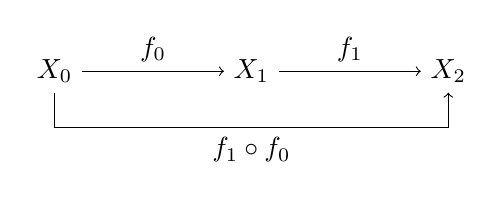
\begin{tikzpicture}[node distance=2.5cm, auto]
	\node (X) {$\bm{X_0}$};
	\node (Y) [right of=X] {$\bm{X_1}$};
	\node (n) [below of=Y,node distance=1cm] {$f_1 \circ f_0$};
	\node (Z) [right of=Y] {$\bm{X_2}$};
	\draw[->] (X) to node {$f_0$} (Y);
	\draw[->] (Y) to node {$f_1$} (Z);
%	\draw[->,bend right] (X) to node[swap] {$g \circ f$} (Z);
	\draw[->] (X) |- (n.90) -| (Z);\
\end{tikzpicture}
\end{figure}
	\end{enumerate}
\end{prop}
\begin{proof}
\begin{enumerate}
	\item Seja $A \in \topo$. Então $\Id_X\inv(A)=A \in \topo$, logo $\Id_x$ é contínua.
	
	\item Seja $A \in \topo_2$. Como $f_1$ é contínua, $f_1\inv(A) \in \topo_1$. Como $f_0$ é contínua, $f_0\inv(f_1\inv(A)) \in \topo_0$. Portanto
	\begin{equation*}
	(f_1 \circ f_0)\inv(A) = f_1\inv \circ f_0\inv (A) = f_0\inv(f_1\inv(A)) \in \topo_0.
	\end{equation*}
Logo $f_1 \circ f_0$ é contínua.
\end{enumerate}
\end{proof}

\subsection{Topologias Induzidas}

Nesta seção estudaremos como induzir topologias em conjuntos a partir de topologias que já temos. Isso será feito, em geral, de modo que uma ou mais funções sejam contínuas e a topologia induzida seja a menor ou a maior possível, dependendo do caso. Quando temos uma função de um conjunto em um espaço topológico, podemos induzir uma topologia nesse conjunto de modo que a topologia faça com  que a função seja contínua. Nesse caso, a maior topologia que faz a função ser contínua é a topologia discreta, e o nosso interesse será achar a menor topologia tal que a função é discreta. Quando temos uma função de um espaço topológico em um conjunto, o caso se inverte. A menor topologia tal que a função é contínua sempre é a topologia trivial, e o nosso interesse está na maior topologia que garante a continuidade. De maneira parecida, podemos induzir topologias garantindo a continuidade de várias funções e também considerando funções injetivas e sobrejetivas quado necessário. O estudo desta seção envolve a definição dessas noções e a investigação inicial como sobre esses objetos se comportam e por que são os menores ou maiores com determinadas características.

\subsubsection{Topologias Puxada e Inicial}

\begin{defi}
Sejam $X$ um conjunto, $\bm Y = (Y,\topo_Y)$ um espaço topológico e $f: X \to Y$ uma função. A \emph{topologia puxada} por $f$ de $\bm Y$ para $X$ é
	\begin{equation*}
	f^\star(\topo_Y) := \set{f^{-1}(A)}{A \in \topo_Y}.
	\end{equation*}
\end{defi}

\begin{prop}
Sejam $X$ um conjunto, $\bm Y = (Y,\topo_Y)$ um espaço topológico e $f: X \to Y$ uma função. Então $f^\star(\topo_Y)$, a topologia puxada por $f$ de $\bm Y$ para $X$, é uma topologia de $X$.
\end{prop}
\begin{proof}
(1) Notemos que, como $\emptyset \in \topo_Y$ e $\emptyset = f\inv(\emptyset)$, temos que $\emptyset \in f^\star(\topo_Y)$. (2) Seja $(A_i)_{i \in I}$ uma família de conjuntos em $f^\star(\topo_Y)$. Então, para cada $i \in I$, existe aberto $U_i \in \topo_Y$ tal que $A_i=f\inv(U_i)$. Como $\topo_Y$ é topologia, a união de abertos é aberto $\bigcup_{i \in I} U_i \in \topo_Y$. Portanto
	\begin{equation*}
	\bigcup_{i \in I} A_i = \bigcup_{i \in I} f\inv(U_i) = f\inv\left( \bigcup_{i \in I} U_i\right),
	\end{equation*}
logo $\bigcup_{i \in I} A_i \in f^\star(\topo_Y)$.
(3) Seja $(A_i)_{i=1}^n$ uma família de conjuntos em $f^\star(\topo_Y)$. Então, para cada $1 \leq i \leq n$, existe aberto $U_i \in \topo_Y$ tal que $A_i=f\inv(U_i)$. Como $\topo_Y$ é topologia, a interseção finita de abertos é aberto $\bigcap_{i=1}^n U_i \in \topo_Y$. Portanto
	\begin{equation*}
	\bigcap_{i=1}^n A_i = \bigcap_{i=1}^n f\inv(U_i) = f\inv\left( \bigcap_{i=1}^n U_i\right),
	\end{equation*}
logo $\bigcap_{i=1}^n A_i \in f^\star(\topo_Y)$.
\end{proof}

\begin{prop}
\label{topo:prop.cont.topo.pux}
Sejam $\bm X = (X,\topo_ X)$ e $\bm Y = (Y,\topo_ Y)$ espaços topológicos. Uma função $f: X \to Y$ é função contínua de $\bm X$ para $\bm Y$ se, e somente se, a topologia $f^\star(\topo_Y)$ puxada por $f$ de $\bm Y$ para $X$ é uma subtopologia de $\topo_ X$.
	\begin{equation*}
	f \in \cont(\bm X,\bm Y) \sse f^\star(\topo_Y) \subseteq \topo_X.
	\end{equation*}
\end{prop}
\begin{proof}
Suponha que $f \in \cont(\bm X,\bm Y)$ e seja $B \in f^\star(\topo_Y)$. Então existe $A \in \topo_Y$ tal que $B=f\inv(A)$. Como $f$ é contínua, segue que $f\inv(A) \in \topo_X$, portanto, $f^\star(\topo_Y) \subseteq \topo_X$. Reciprocamente, suponha que $f^\star(\topo_Y) \subseteq \topo_X$. Então, para todo $A \in \topo_Y$, $f\inv(A) \in f^\star(\topo_Y)$, portanto $f\inv(A) \in \topo_X$, o que mostra que $f \in \cont(\bm X,\bm Y)$.
\end{proof}

\begin{defi}
Sejam $\bm X$ um conjunto, $(\bm{X_i})_{i \in I} = (X_i,\topo_i)_{i \in I}$ uma família de espaços topológicos e, para todo $i \in I$, $f_i: X \to X_i$ uma função. A \emph{topologia inicial} de $X$ com respeito à família $(f_i)_{i \in I}$ é a menor topologia de $X$ tal que, para todo $i \in I$, $f_i$ é contínua.
\end{defi}

\begin{prop}
Sejam $\bm X$ um conjunto, $(\bm{X_i})_{i \in I} = (X_i,\topo_i)_{i \in I}$ uma família de espaços topológicos e, para todo $i \in I$, $f_i: X \to X_i$ uma função. A topologia inicial de $X$ com respeito à família $(f_i)_{i \in I}$ é a topologia
	\begin{equation*}
	\ger{\bigcup_{i \in I} {f_i}^\star(\topo_i)}.
	\end{equation*}
\end{prop}
\begin{proof}
Seja $\topo$ uma topologia de $X$ tal que, para todo $i \in I$, $f_i: X \to X_i$ é contínua. Então, para todo $i \in I$, ${f_i}^\star(\topo_i) \subseteq \topo$ (\ref{topo:prop.cont.topo.pux}), o que implica que $\bigcup_{i \in I} {f_i}^\star(\topo_i) \subseteq \topo$ e, portanto, $\ger{\bigcup_{i \in I} {f_i}^\star(\topo_i)} \subseteq \topo$.
\end{proof}

\subsubsection{Topologias Empurrada e Final}

\begin{defi}
Sejam $\bm X = (X,\topo_X)$ um espaço topológico, $Y$ um conjunto e $f: X \to Y$ uma função. A \emph{topologia empurrada} por $f$ de $\bm X$ para $Y$ é
	\begin{equation*}
	f_\star(\topo_X) := \set{A \subseteq Y}{f^{-1}(A) \in \topo_X}.
	\end{equation*}
\end{defi}

\begin{prop}
Sejam $\bm X = (X,\topo_X)$ um espaço topológico, $Y$ um conjunto e $f: X \to Y$ uma função. Então $\topo_Y := f_\star(\topo_X)$, a topologia empurrada por $f$ de $\bm X$ para $Y$, é uma topologia de $Y$.
\end{prop}
\begin{proof}
(1) Como $f\inv(\emptyset)=\emptyset$ e $f\inv(Y)=X$, segue que $\emptyset,Y \in f_\star(\topo_X)$. (2) Seja $(A_i)_{i \in I}$ uma família de conjuntos de $f_\star(\topo_X)$. Então, para cada $i \in I$, $f\inv(A_i) \in \topo_X$, o que implica que
\begin{equation*}
	f\inv \left( \bigcup_{i \in I} A_i \right) = \bigcup_{i \in I} f\inv(A_i) \in \topo_X,
	\end{equation*}
portanto $\bigcup_{i \in I} A_i \in f_\star(\topo_X)$. (3) Seja $(A_i)_{i=1}^n$ uma família de conjuntos de $f_\star(\topo_X)$. Então, para cada $1 \leq i \leq n$, $f\inv(A_i) \in \topo_X$, o que implica que
\begin{equation*}
	f\inv \left( \bigcap_{i=1}^n A_i \right) = \bigcap_{i=1}^n f\inv(A_i) \in \topo_X,
	\end{equation*}
portanto $\bigcap_{i=1}^n A_i \in f_\star(\topo_X)$.
\end{proof}

\begin{defi}
Sejam $\bm X$ um conjunto, $(\bm{X_i})_{i \in I} = (X_i,\topo_i)_{i \in I}$ uma família de espaços topológicos e, para todo $i \in I$, $f_i: X_i \to X$ uma função. A \emph{topologia final} de $X$ com respeito à família $(f_i)_{i \in I}$ é a maior topologia de $X$ tal que, para todo $i \in I$, $f_i$ é contínua.
\end{defi}

\begin{prop}
Sejam $\bm X$ um conjunto, $(\bm{X_i})_{i \in I} = (X_i,\topo_i)_{i \in I}$ uma família de espaços topológicos e, para todo $i \in I$, $f_i: X_i \to X$ uma função. A topologia final de $X$ com respeito à família $(f_i)_{i \in I}$ é a topologia
	\begin{equation*}
	\bigcap_{i \in I} {f_i}_\star(\topo_i).
	\end{equation*}
\end{prop}
\begin{proof}
Seja $\topo$ uma topologia de $X$ tal que, para todo $i \in I$, $f_i: X_i \to X$ é contínua, e seja $A \in \topo$. Então, para todo $i \in I$, $f_i \inv(A) \in \topo_i$, o que implica que $A \in {f_i}_\star(\topo_i)$, portanto $A \in \bigcap_{i \in I} {f_i}_\star(\topo_i)$. Isso mostra que $\topo \subseteq \bigcap_{i \in I} {f_i}_\star(\topo_i)$, e como interseção de topologiaas é topologia, segue o procurado.
\end{proof}

\subsubsection{Produto de Espaços Topológicos}

\begin{defi}
Seja $(\bm{X_i})_{i \in I} = (X_i,\topo_i)_{i \in I}$ uma família de espaços topológicos. O \emph{produto} da família $(\bm{X_i})_{i \in I}$ é o par
	\begin{equation*}
	\prod_{i \in I} \bm{X_i} := \left( \prod_{i \in I} X_i , \ger{\bigcup_{i \in I}{\pi_i}^\star(\topo_i)} \right).
	\end{equation*}
A topologia $\ger{\bigcup_{i \in I}{\pi_i}^\star(\topo_i)}$ é a \emph{topologia produto} de $\prod_{i \in I} X_i$.
\end{defi}

\begin{prop}
Sejam $(\bm{X_i})_{i \in I} = (X_i,\topo_i)_{i \in I}$ uma família de espaços topológicos e $X = \prod_{i \in I} X_i$ o produto de conjuntos. A topologia produto de $X$ é a topologia gerada pela base cujos elementos são $\prod_{i \in I} A_i$, tal que $A_i \in \topo_i$ e existe $J \subseteq I$ finito com $A_i = X_i$ para $i \in I \setminus J$.
\end{prop}
\begin{proof}
Como $\pi_i = \pi_i \circ \Id_X$, segue de uma propriedades básica de imagem inversa de produto (\ref{conj:prop.im.inv.prod}) que
	\begin{equation*}
	\prod_{i \in I} A_i = \Id_X\inv \left(\prod_{i \in I} A_i\right) = \bigcap_{i \in I} \pi_i\inv(A_i)
	\end{equation*}
Para todo $i \in I \setminus J$, $A_i=X_i$, então $\pi_i\inv(A_i)=X$ e, portanto,
	\begin{equation*}
	\bigcap_{i \in I\setminus J} \pi_i\inv(A_i) = \bigcap_{i \in I\setminus J} X = X.
	\end{equation*}
Isso implica que
	\begin{equation*}
	\bigcap_{i \in I} \pi_i\inv(A_i) = \left(\bigcap_{i \in I\setminus J} \pi_i\inv(A_i)\right) \cap \left(\bigcap_{j \in J} \pi_j\inv(A_j)\right) =  \bigcap_{j \in J} \pi_j\inv(A_j)
	\end{equation*}
Logo $\prod_{i \in I} A_i = \bigcap_{j \in J} \pi_j\inv(A_j)$. Seja $A$ aberto da topologia descrita na proposição. Então
	\begin{equation*}
	A = \bigcup_{k \in K} A_k = \bigcup_{k \in K}\prod_{i \in I} A_{ki} = \bigcup_{k \in K}\bigcap_{j \in J} \pi_j\inv (A_{kj}),
	\end{equation*}
o que mostra que $A$ é aberto da topologia produto. O resto da demonstração é simples.
\end{proof}

\begin{prop}[Propriedade Universal]
Sejam $(\bm{X_i})_{i \in I} = (X_i,\topo_i)_{i \in I}$ uma família de espaços topológicos, $\bm T = (T,\topo_T)$ um espaço topológico e, para todo $i \in I$, $f_i: \bm T \to \bm{X_i}$ uma função contínua. Então existe uma única função contínua $f: \bm T \to \prod_{i \in I} \bm{X_i}$ tal que, para todo $i \in I$, $\pi_i \circ f = f_i$ (o diagrama comuta).
\begin{figure}
\centering
\begin{tikzpicture}[node distance=2.5cm, auto]
	\node (P) {$\displaystyle\prod_{i \in I} \bm{X_i}$};
	\node (Ci) [below of=P] {$\bm{X_i}$};
	\node (X) [left of=Ci] {$\bm{T}$};
	\draw[->] (X) to node [swap] {$f_i$} (Ci);
	\draw[->, dashed] (X) to node {$f$} (P);
	\draw[->] (P) to node {$\pi_i$} (Ci);
\end{tikzpicture}
\end{figure}
\end{prop}
\begin{defi}
Defina a função
	\begin{align*}
	\func{f}{T}{ \prod_{i \in I} X_i}{ x}{ (f_i(x))_{i \in I}}.
	\end{align*}
Pela propriedade universal do produto de conjuntos, $f$ é única e $\pi_i \circ f = f_i$. Resta mostrar que $f$ é contínua. Seja $A \in \topo_X$. Então $A=\bigcup_{k \in K} A_k$ é uma união de abertos básicos $A_k \in \topo$. Isso significa que, para todo $k \in K$, $A_k = \prod_{i \in I} A_{ki}$, com $A_{ki} \in \topo_i$ para todo $i \in I$ e existe $J_k \subseteq I$ finito tal que, para todo $i \in I \setminus J_k$, $A_{ki} = X_i$. Assim, por propriedades básicas de imagem inversa de união e produto (\ref{conj:prop.im.inv.prod}),
		\begin{equation*}
		f\inv(A) = f\inv\left(\bigcup_{k \in K}\prod_{i \in I} A_{ki}\right) = \bigcup_{k \in K} f\inv \left( \prod_{i \in I} A_{ki} \right) = \bigcup_{k \in K}\bigcap_{i \in I}f_i\inv(A_{ki}).
		\end{equation*}
Seja $k \in K$. Como, para todo $i \in I \setminus J_k$, $A_{ki} = X_i$, então $f_i\inv(A_{ki}) = f_i\inv(X_i) = T$. Disso segue que
	\begin{equation*}
	\bigcap_{i \in I}f_i\inv(A_{ki}) = \bigcap_{j \in J_k}f_j\inv(A_{kj})
	\end{equation*}
e, portanto,
	\begin{equation*}
	f\inv(A) = \bigcup_{k \in K}\bigcap_{j \in J_k}f_j\inv(A_{kj}).
	\end{equation*}
Seja $k \in K$. Para todo $j \in J_k$, $f_j$ é contínua, o que impica que $f_j\inv(A_{kj})$ é aberto e, por $J_k$ ser finito, a interseção $\bigcap_{j \in J_k}f_j\inv(A_{kj})$ é aberta. Isso significa que a união $\bigcup_{k \in K}\bigcap_{j \in J_k}f_j\inv(A_{kj})$ é aberta e, portanto, $f\inv(A) \in \topo_T$. Logo $f$ é contínua.
\end{defi}

\subsubsection{Coproduto de Espaços Topológicos}

\begin{defi}
Seja $(\bm{X_i})_{i \in I} = (X_i,\topo_i)_{i \in I}$ uma família de espaços topológicos. O \emph{coproduto} da família $(\bm{X_i})_{i \in I}$ é o par
	\begin{equation*}
	\coprod_{i \in I} \bm{X_i} := \left( \coprod_{i \in I} X_i , \bigcap_{i \in I}{\iota_i}_\star(\topo_i) \right).
	\end{equation*}
A topologia $\bigcap_{i \in I}{\pi_i}_\star(\topo_i)$ é a \emph{topologia coproduto} de $\coprod_{i \in I} X_i$.
\end{defi}

\begin{prop}[Propriedade Universal]
Sejam $(\bm{X_i})_{i \in I} = (X_i,\topo_i)_{i \in I}$ uma família de espaços topológicos, $\bm T = (T,\topo_T)$ um espaço topológico e, para todo $i \in I$, $f_i: \bm{X_i} \to \bm T$ uma função contínua. Então existe uma única função contínua $f: \coprod_{i \in I} \bm{X_i} \to \bm T$ tal que, para todo $i \in I$, $f \circ \iota_i = f_i$ (o diagrama comuta).
\begin{figure}
\centering
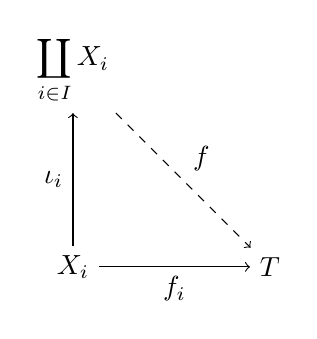
\begin{tikzpicture}[node distance=2.5cm, auto]
	\node (Ci) {$\bm{X_i}$};
	\node (S) [above of=Ci] {$\displaystyle\coprod_{i \in I} \bm{X_i}$};
	\node (X) [right of=Ci] {$\bm T$};
	\draw[->] (Ci) to node [swap] {$f_i$} (X);
	\draw[->, dashed] (S) to node {$f$} (X);
	\draw[->] (Ci) to node {$\iota_i$} (S);
\end{tikzpicture}
\end{figure}
\end{prop}

\subsubsection{Subespaços Topológicos}

\begin{defi}
Sejam $(X,\topo)$ um espaço topológico e $S \subseteq X$ um subconjunto. A \emph{topologia induzida} por $\topo$ em $S$ é o conjunto
	\begin{equation*}
	\topo|_S := \set{A \cap S}{A \in \topo}.
	\end{equation*}
\end{defi}

\begin{prop}
Sejam $(X,\topo)$ um espaço topológico e $S \subseteq X$ um subconjunto. A topologia induzida por $\topo$ em $S$ é o conjunto
	\begin{equation*}
	\topo|_S = \iota_\star(\topo),
	\end{equation*}
a maior topologia tal que a inclusão $\iota: S \to X$ é contínua.
\end{prop}

\begin{prop}
Sejam $(X,\topo)$ um espaço topológico e $S \subseteq X$ um subconjunto. A topologia induzida por $\topo$ em $S$ é uma topologia de $S$.
\end{prop}
\begin{proof}
(1) Notemos que $\emptyset,Y \in \topo|_Y$, pois $\emptyset \cap Y = \emptyset$ e $X \cap Y = Y$. (2) Seja $(A_i)_{i \in I}$ uma família de abertos de $\topo|_Y$. Então, para cada $i \in I$, existe um aberto $B_i \in \topo$ tal que $A_i = B_i \cap Y$. Assim, temos que
	\begin{equation*}
	\bigcup_{i \in I} A_i = \bigcup_{i \in I} (B_i \cap Y) = \left( \bigcup_{i \in I} B_i \right) \cap Y,
	\end{equation*}
que pertence à topologia induzida pois $\bigcup_{i \in I} B_i \in \topo$. (3) Seja $(A_i)_{i=1}^n$ uma família de abertos de $\topo|_Y$. Então, para cada $1 leq i leq n$, existe um aberto $B_i \in \topo$ tal que $A_i = B_i \cap Y$. Assim, temos que
	\begin{equation*}
	\bigcap_{i=1}^n A_i = \bigcap_{i=1}^n (B_i \cap Y) = \left( \bigcap_{i=1}^n B_i \right) \cap Y,
	\end{equation*}
que pertence à topologia induzida pois $\bigcap_{i=1}^n B_i \in \topo$.
\end{proof}

\begin{prop}[Propriedade característica]
Sejam $\bm X=(X,\topo_X)$ e $(Y,\topo_Y)$ espaços topológicos e $\bm S \subseteq \bm X$ um subespaço. Uma função $f: Y \to S$ é contínua se, e somente se, $\iota \circ f: Y \to X$ é contínua (o diagrama comuta).
\begin{figure}
\centering
\begin{tikzpicture}[node distance=2.5cm, auto]
	\node (X) {$\bm X$};
	\node (S) [below of=X] {$\bm S$};
	\node (Y) [left of=S] {$\bm{T}$};
	\draw[->] (Y) to node [swap] {$f$} (S);
	\draw[->] (Y) to node {$\iota \circ f$} (X);
	\draw[->] (S) to node [swap] {$\iota$} (X);
\end{tikzpicture}
\end{figure}
\end{prop}

\paragraph*{Proposição} Restrição de função contínua é contínua na topologia induzida.

\begin{prop}[Colagem por abertos]
Sejam $\bm X$ e $\bm Y$ espaços topológicos, $f: X \to Y$ uma função e $(X_i)_{i \in I}$ uma cobertura de $X$ por conjuntos abertos tal que, para todo $i \in I$, $f|_{X_i}: X_i \to Y$ é contínua. Então $f: X \to Y$ é contínua.
\end{prop}

\begin{prop}[Colagem por fechados]
Sejam $\bm X$ e $\bm Y$ espaços topológicos, $f: X \to Y$ uma função e $(X_i)_{i=1}^n$ uma cobertura de $X$ por conjuntos fechados tal que, para todo $1 \leq i \leq n$, $f|_{X_i}: X_i \to Y$ é contínua. Então $f: X \to Y$ é contínua.
\end{prop}

\subsubsection{Quociente de Espaços Topológicos}

\begin{defi}
Sejam $\bm X = (X,\topo)$ um espaço topológico e $\sim$ uma relação de equivalência em $X$. O \emph{espaço quociente} com respeito a $\sim$ é o espaço topológico
	\begin{equation*}
	\bm{\quo{X}{\sim}} := \left( \quo{X}{\sim}, \pi^\star(\topo) \right),
	\end{equation*}
em que $\pi: X \to \quo{X}{\sim}$ é a projeção canônica de equivalências.
\end{defi}

É fácil notar que os abertos de $\bm{\quo{X}{\sim}}$ são conjuntos de classes de equivalência cuja união é um aberto de $\bm X$. Notemos, ainda, que se $f: X \to Y$ é sobrejetivo, existe uma relação de equivalência em $X$ induzida por $f$, definida como dois elementos são equivalentes se suas imagens são iguais, e essa relação de equivalência faz com que possamos identificar $Y$ com $\quo{X}{\sim}$ como conjuntos. Definimos a topologia em $Y$ de modo que $Y$ e $\quo{X}{\sim}$ sejam homeomorfos.

\begin{prop}[Propriedade característica]
Sejam $\bm X=(X,\topo_X)$ e $(Y,\topo_Y)$ espaços topológicos e $\bm Q$ um espaço quociente de $\bm X$. Uma função $f: Q \to Y$ é contínua se, e somente se, $f \circ \pi: X \to Y$ é contínua (o diagrama comuta).
\begin{figure}
\centering
\begin{tikzpicture}[node distance=2.5cm, auto]
	\node (Q) {$\bm Q$};
	\node (X) [above of=Q] {$\bm X$};
	\node (Y) [right of=Q] {$\bm Y$};
	\draw[->] (Q) to node [swap] {$f$} (Y);
	\draw[->] (X) to node {$f \circ \pi$} (Y);
	\draw[->] (X) to node [swap] {$\pi$} (Q);
\end{tikzpicture}
\end{figure}
\end{prop}


\section{Separação}

\subsection{Noções de Separação de Conjuntos}

Nesta seção são apresentadas algumas noções de como dois conjuntos de um espaço topológico podem ser separadas. As duas noções mas simples de separação são noções conjuntistas. A primeira é a de conjuntos distintos, ou diferentes, $A \neq B$, e a outra é a de conjuntos disjuntos, $A \cap B = \emptyset$. A seguir, mostramos noções que envolvem construções topológicas e não meramente conjuntistas.

\begin{defi}
Sejam $\bm X$ um espaço topológico e $A,B \subseteq X$. Definimos as seguintes relações entre $A$ e $B$:
	\begin{enumerate}
	\item (\emph{Separação}) Cada conjunto é disjunto do feixo do outro.
	\begin{equation*}
	A \cap \Fec{B} = \Fec{A} \cap B = \emptyset.
	\end{equation*}
	\item (\emph{Separação por vizinhanças}) Existem vizinhanças $V_A \in \viz_A$ e $V_B \in \viz_B$ que são disjuntas.
	\begin{equation*}
	V_A \cap V_B = \emptyset.
	\end{equation*}
	\item (\emph{Separação por função contínua}) Existe uma função contínua $f \in \cont(X,[0,1])$ tal que
	\begin{equation*}
	f(A)=\{0\} \e f(B)=\{1\}.
	\end{equation*}
	\item (\emph{Separação precisa por função contínua}) Existe uma função contínua $f \in \cont(X,[0,1])$ tal que
	\begin{equation*}
	f\inv(\{0\})=A \e f\inv(\{1\})=B.
	\end{equation*}
	\end{enumerate}
Cada uma das relações vale entre pontos $x,y \in X$, ou entre um conjunto $A$ e um ponto $x$, ao considerarmos no lugar no ponto o conjunto unitário que o contém: valem entre os conjuntos $\{x\}$ e $\{y\}$, ou entre $A$ e $\{x\}$, respectivamente.
\end{defi}

	As primeiras duas relações binárias são claramente simétricas, mas isso não é necessariamente claro no caso da terceira e quarta. No entanto, isso pode ser concluído ao cosiderar, dada uma função $f$ que faz $A$ e $B$ separados por função contínua, a função $1-f$ que faz o mesmo entre $B$ e $A$.

\begin{prop}
\label{topo:prop.separacao}
Sejam $\bm X$ um espaço topológico e $A,B \subseteq X$. Então
	\begin{enumerate}
	\item Se $A$ e $B$ são precisamente separados por função contínua, então são separados por função contínua.
	\item Se $A$ e $B$ são separados por função contínua, então são separados por vizinhanças.
	\item Se $A$ e $B$ são separados por vizinhanças, então são separados.
	\item Se $A$ e $B$ são separados, então são disjuntos.
	\end{enumerate}
\end{prop}
%\begin{proof}
%Suponhamos que existe função contínua $f:X \to [0,1]$ tal que $f(A)= \{0\}$ e $f(B)=\{1\}$. Definamos $U := f^{-1}(\left[0,\frac{1}{2}\right))$ e $V := f^{-1}((\frac{1}{2},1))$. Como $f$ é contínua, $U$ e $V$ são abertos. Ainda, $A \subseteq U$ e $B \subseteq V$. Por fim, como $U \cap V = \emptyset$, concluímos que $\bm X$ é normal.
%\end{proof}

% DÚVIDA: As relações de separação negadas são relações de equivalência? Pois indintinguibilidade topológica é, e ela é a negação de separação de pontos (não exatamente). Tentar entender melhor isso.


\subsection{Espaços Distinguíveis}

\begin{defi}
Seja $\bm X$ um espaço topológico. Pontos \emph{topologicamente indistinguíveis} em $\bm X$ são pontos $x,y \in X$ tais que $\viz_x = \viz_y$. Pontos \emph{topologicamente disntinguíveis em $\bm X$} são pontos que não são topologicamente indistinguíveis.
\end{defi}

\begin{prop}
Seja $\bm X$ um espaço topológico. A relação binária de indistinguibilidade topológica é uma relação de equivalência em $X$.
\end{prop}
\begin{proof}
Denotemos por $\sim$ a relação binária de indistinguibilidade topológica. Sejam $x,y,z \in X$. Para mostrar a reflexividade, notemos que, como $\viz_x=\viz_y$, então $x \sim x$. Para mostrar a simetria, se $x \sim y$, então $\viz_x=\viz_y$, o que é equivalente a $\viz_y=\viz_x$ e, portanto, $y \sim x$. Por fim, para mostrar a transitividade, se $x \sim y$ e $y \sim z$, então $\viz_x=\viz_y$ e $\viz_y=\viz_z$, o que implica $\viz_x=\viz_z$ e, portanto, $x \sim z$.
\end{proof}

O fato de que essa é uma relação de equivalência mostra que podemos obter a partir de qualquer espaço topológico um espaço topológico em que nenhum ponto é topologicamente indisntinguível. Para isso, basta considerar o espaço quociente definido pela relação. de indistinguibilidade topológica. Espaços com essa propriedade são definidos a seguir.

\begin{defi}[$T_0$]
Um espaço topológico \emph{distinguível} é um espaço topológico $\bm X$ em que todo par de pontos distintos é topologicamente distinguível:
	\begin{equation*}
	\forall x,y \in X \quad x \neq y \quad \Rightarrow \quad \viz_x \neq \viz_y.
	\end{equation*}
\end{defi}

\begin{prop}
Seja $\bm X$ um espaço topológico. São equivalentes as seguites propriedades:
	\begin{enumerate}
	\item $\bm X$ é dinstinguível.
	\item $\forall x,y \in X \quad x \neq y \quad \Rightarrow \quad \viz_x \nsubseteq \viz_y \ou \viz_y \nsubseteq \viz_x$.
	\item $\forall x,y \in X \quad x \neq y \quad \Rightarrow \quad x \notin \Fec{\{y\}} \ou y \notin \Fec{\{x\}}$.
	\item $\forall x,y \in X \quad x \neq y \quad \Rightarrow \quad \Fec{\{x\}} \neq \Fec{\{y\}}$.	
\end{enumerate}
\end{prop}

\begin{prop}
Sejam $\bm X$ um espaço topológico distinguível e $Y \subseteq X$. Então $\bm Y$ é um espaço topológico distinguível.
\end{prop}

\begin{prop}
Seja $(X_i)_{i \in I}$ uma família não vazia de espaços topológicos não vazios. O espaço produto $\prod_{i \in I} \bm{X_i}$ é distinguível se, e somente se, todos os espaços $\bm X_i$ são distinguíveis.
\end{prop}

\subsection{Espaços Acessíveis}

\begin{defi}[$T_1$]
Um espaço topológico \emph{acessível} é um espaço topológico $\bm X$ em que
	\begin{equation*}
	\forall x,y \in X \quad x \neq y \quad \Rightarrow \quad \viz_x \nsubseteq \viz_y \e \viz_y \nsubseteq \viz_x.
	\end{equation*}
\end{defi}

\begin{prop}[$T_1 \Rightarrow T_0$]
Seja $\bm X$ um espaço topológico. Se $\bm X$ é acessível, então $\bm X$ é dintinguível.
\end{prop}
\begin{proof}
Se $\bm X$ é acessível, então, para todos $x,y \in X$ tais que $x \neq y$, temos que $\viz_x \nsubseteq \viz_y \e \viz_y \nsubseteq \viz_x$. Mas isso implica que $\viz_x \nsubseteq \viz_y \ou \viz_y \nsubseteq \viz_x$, o que é equivalente a $\viz_x \neq \viz_y$. Logo $\bm X$ é dintinguível.
\end{proof}

\begin{prop}
Seja $\bm X$ um espaço topológico. São equivalentes as seguintes propriedades:
	\begin{enumerate}
	\item $\bm X$ é acessível.
	\item Todo par de pontos distintos é separado:
		\begin{equation*}
		\forall x,y \in X \quad x \neq y \quad \Rightarrow \quad x \notin \Fec{\{y\}} \e y \notin \Fec{\{x\}}.
		\end{equation*}
	\item $\forall x,y \in X \quad x \neq y \quad \Rightarrow \quad \exists U \in \viz_x,\ V \in \viz_y \qquad y \notin U \e x \notin V$.
	\item $\forall x \in X \quad \Fec{\{x\}}=\{x\}$.
	\end{enumerate}
\end{prop}

\begin{prop}
Sejam $\bm X$ um espaço topológico acessível e  $Y \subseteq X$. Então $\bm Y$ é um espaço topológico acessível.
\end{prop}

\begin{prop}
Seja $(X_i)_{i \in I}$ uma família não vazia de espaços topológicos não vazios. O espaço produto $\prod_{i \in I} \bm{X_i}$ é acessível se, e somente se, todos os espaços $\bm X_i$ são acessíveis.
\end{prop}

\subsection{Espaços Separados por Vizinhanças}

\begin{defi}[$T_2$]
Um espaço topológico \emph{separado por vizinhanças} é um espaço topológico $\bm X$ em que todo par de pontos distintos é separado por vizinhanças:
	\begin{equation*}
	\forall x,y \in X \quad x \neq y \quad \Rightarrow \quad \exists U \in \viz_x,\ V \in \viz_y \quad U \cap V = \emptyset.
	\end{equation*}
\end{defi}
Esses espaços também são conhecidos como espaços de Hausdorff.

\begin{prop}[$T_2 \Rightarrow T_1$]
Seja $\bm X$ um espaço topológico. Se $\bm X$ é separado por vizinhanças, então $\bm X$ é acessível.
\end{prop}

\begin{prop}
Seja $\bm X$ um espaço topológico. São equivalentes as seguintes propriedades:
	\begin{enumerate}
	\item $\bm X$ é separado por vizinhanças.
	\item Toda rede convergente em $\bm X$ tem limite único.
	\item Todo filtro convergente em $\bm X$ tem limite único.
	\end{enumerate}
\end{prop}

\begin{prop}
Sejam $\bm X$ um espaço topológico separado por vizinhanças e $Y \subseteq X$. Então $\bm Y$ é um espaço topológico separado por vizinhanças.
\end{prop}

\begin{prop}
Seja $(\bm X_i)_{i \in I}$ uma família não vazia de espaços topológicos não vazios. O espaço produto $\prod_{i \in I} \bm{X_i}$ é separado por vizinhanças se, e somente se, todos os espaços $\bm X_i$ são separados por vizinhanças.
\end{prop}

\begin{prop}
Sejam $\bm X$ um espaço topológico, $\bm Y$ um espaço topológico separado por vizinhanças, $D \subseteq X$ um subconjunto denso em $X$ e $f,g: X \to Y$ funções contínuas tais que $f|_D=g|_D$. Então $f=g$.
\end{prop}

\subsection{Espaços Regulares}

\begin{defi}
Um espaço topológico \emph{regular} é um espaço topológico
% $\bm X$
em que é possível separar por vizinhanças qualquer ponto de qualquer conjunto fechado que não o contém.
%: para todo $x \in X$ e para todo conjunto fechado $F \subseteq X$,
%	\begin{equation*}
%	F \cap \{x\}=\emptyset \quad \Rightarrow \quad \exists U \in \viz_x, \exists V \in \viz_F \quad U \cap V = \emptyset.
%	\end{equation*}
\end{defi}

Espaços seprados regulares são também chamados de $T_3$.

\begin{prop}
Seja $\bm X$ um espaço topológico regular. Então $\bm X$ é separado por vizinhanças se, e somente se, é distinguível.
\end{prop}
\begin{proof}
Sabemos que todo espaço separado por vizinhanças é distinguível. Para demonstrar a recíproca, supondo que $\bm X$ é distinguível, então para todos pontos $x,y \in X$, $x \notin \Fec{\{y\}}$ ou $y \notin \Fec{\{x\}}$. Sem perda de generalidade, assumamos o primeiro caso. Seja $F := \Fec{\{y\}}$. Então $F$ é fechado e $x \notin F$. Da regularidade de $\bm X$, segue que existem $U \in \viz_x$ e $V \in \viz_{F}$ tais que $U \cap V = \emptyset$. Como $y \in F$, então $V \in \viz_y$, o que implica que $\bm X$ é separado por vizinhanças.
\end{proof}

\begin{prop}
Seja $\bm X$ um espaço topológico. São equivalentes as seguintes propriedades:
	\begin{enumerate}
	\item $\bm X$ é regular.
	\item Para todos ponto $x \in X$ e aberto $A \in \viz_x$, existe aberto $V \in \viz_x$ tal que
		\begin{equation*}
		x \in V \subseteq \Fec{V} \subseteq A.
		\end{equation*}
	\end{enumerate}
\end{prop}

\begin{prop}
Sejam $\bm X$ um espaço topológico regular e $Y \subseteq X$. Então $\bm Y$ é um espaço topológico regular.
\end{prop}

\begin{prop}
Seja $(X_i)_{i \in I}$ uma família não vazia de espaços topológicos não vazios. O espaço produto $\prod_{i \in I} \bm{X_i}$ é regular se, e somente se, todos os espaços $\bm X_i$ são regulares.
\end{prop}

\subsection{Espaços Completamente Regulares}

\begin{defi}
Um espaço topológico \emph{completamente regular} é um espaço topológico
% $\bm X$
em que é possível separar por função contínua qualquer ponto de qualquer conjunto fechado que não o contém.
%: para todo $x \in X$ e para todo conjunto fechado $F \subseteq X$,
%	\begin{equation*}
%	\{x\} \cap F=\emptyset \quad \Rightarrow \quad \exists f \in \mathcal{C}(X,[0,1]) \quad f(x)=\{0\} \e f(F)=\{1\}.
%	\end{equation*}
\end{defi}

\begin{prop}
Seja $\bm X$ um espaço topológico. Se $\bm X$ é completamente regular, então $\bm X$ é regular.
\end{prop}

\begin{prop}
Sejam $\bm X$ um espaço topológico completamente regular e $Y \subseteq X$. Então $\bm Y$ é um espaço topológico completamente regular.
\end{prop}

\begin{prop}
Seja $(X_i)_{i \in I}$ uma família não vazia de espaços topológicos não vazios. O espaço produto $\prod_{i \in I} \bm{X_i}$ é completamente regular se, e somente se, todos os espaços $\bm X_i$ são completamente regulares.
\end{prop}

\subsection{Espaços Normais}

\begin{defi}
Um espaço topológico \emph{normal} é um espaço topológico
% $\bm X$ 
em que todo par de conjuntos fechados disjuntos é separado por vizinhanças.
% : para todos fechados $F,G \subseteq X$,
%	\begin{equation*}
%	F \cap G = \emptyset \quad \Rightarrow \quad \exists U \in \viz_F,\ V \in \viz_G \quad U \cap V = \emptyset.
%	\end{equation*}
\end{defi}

Espaços normais separados por vizinhanças são também chamados de $T_4$.

\begin{prop}
Seja $\bm X$ um espaço topológico normal. Então $\bm X$ é separado por vizinhanças se, e somente se, é acessível.
\end{prop}
\begin{proof}
Sabemos que todo espaço separado por vizinhanças é distinguível. Para demonstrar a recíproca, suponhamos que $\bm X$ é acessível e sejam $x,y \in X$ tais que $x \neq y$. Então vale que $\Fec{\{x\}}=\{x\}$ e $\Fec{\{y\}}=\{y\}$. Como $x \neq y$, da normalidade de $\bm X$ existem $V_x \in \viz_x$ e $V_y \in \viz_y$ tais que $V_x \cap V_y = \emptyset$; ou seja, $\bm X$ é separado por vizinhanças.
\end{proof}

\begin{prop}
Sejam $\bm X$ um espaço topológico normal e $Y \subseteq X$ fechado. Então $\bm Y$ é um espaço topológico normal.
\end{prop}

\begin{prop}
Seja $\bm X$ um espaço topológico. São equivalentes as seguintes propriedades:
	\begin{enumerate}
	\item $\bm X$ é normal.
	\item Para todos fechado $F$ e aberto $A \in \viz_F$, existe aberto $V \in \viz_F$ tal que
		\begin{equation*}
		F \subseteq V \subseteq \Fec{V} \subseteq A.
		\end{equation*}
	\end{enumerate}
\end{prop}

\begin{prop}[Lema de Urysohn]
Um espaço topológico $\bm X$ é normal se, e somente se, todo par de conjuntos fechados disjuntos é separado por função contínua.
% : para todos conjuntos fechados $F,G \subseteq X$,
%	\begin{equation*}
%	F \cap G = \emptyset \quad \Rightarrow \quad \exists f \in \mathcal{C}(X,[0,1]) \quad f(F)=\{0\} \e f(G)=\{1\}.
%	\end{equation*}
\end{prop}
\begin{proof}
Se todo par de cojuntos fechados é separado por função contínua, segue da proposição \ref{topo:prop.separacao} que eles são separados por vizinhanças.
%Primeiro, suponhamos que existe função contínua $f:X \to [0,1]$ tal que $f(F)= \{0\}$ e $f(G)=\{1\}$. Definamos $U := f^{-1}(\left[0,\frac{1}{2}\right))$ e $V := f^{-1}((\frac{1}{2},1))$. Como $f$ é contínua, $U$ e $V$ são abertos. Ainda, $F \subseteq U$ e $G \subseteq V$. Por fim, como $U \cap V = \emptyset$, concluímos que $\bm X$ é normal.

Para demonstrar a recíproca, suponhamos que $\bm X$ é normal. Sejam $F_0,F_1 \subseteq X$ conjuntos fechados disjuntos. Seja $Q := \Q \cap \left[0,1\right]$. Construiremos uma família de abertos $(A_q)_{q \in Q}$ com a seguinte propriedade:
	\begin{itemize}
	\item Se $p,q \in Q$ são racionais tais que $p<q$, então $\Fec{A_p} \subseteq A_q$.
	\end{itemize}

Consideremos uma enumeração de $r: \N \to Q$ tal que $r(0)=0$ e $r(1)=1$, de modo que possamos fazer indução nos elementos de $Q$. Definimos $A_1:={F_1}^\complement$ e notamos que $F_0 \subseteq A_1$, pois $F_0$ e $F_1$ são disjuntos. Como $\bm X$ é normal e $F_0 \subseteq A_1$, existe aberto $A_0$ tal que
	\begin{equation*}
	F_0 \subseteq A_0 \subseteq \Fec{A_0} \subseteq A_1.
	\end{equation*}
Mostremos por indução que para todo $q \in Q$ existe $A_q$ com a propriedade enunciada. O caso base já está mostrado pela construção de $A_0$ e $A_1$, então consideremos o passo indutivo. Seja $Q_n := \set{r(k)}{k \in \{0,\ldots,n\}}$ e suponha que $\Fec{A_p} \subseteq A_q$ para todos racionais $p,q \in Q_n$ tais que $p<q$. Consideremos $r=r(n+1) \in Q$. O conjunto $Q_{n+1}$ é um subconjunto finito de $Q$ e, com essa ordem, todo elemento do conjunto tem um antecessor e um sucessor imediatos. Sejam $p,q \in Q_{n+1}$ tais racionais satisfazendo $p<r<q$. Os conjuntos abertos $A_p$ e $A_q$ já estão definidos pela hipótese de indução, então pela normalidade segue que existe aberto $A_r \subseteq X$ tal que
	\begin{equation*}
	\Fec{A_p} \subseteq A_r \subseteq \Fec{A_r} \subseteq A_q.
	\end{equation*}
Mostremos que a propriedade vale para todos elementos de $Q_{n+1}$. Se $p,q \in Q_n$, a propriedade vale. Consideremos $r=r(n+1)$ e $s \in Q_n$. Se $s<r(n+1)$, então $s \leq p$, portanto $\Fec{A_s} \subseteq \Fec{A_p} \subseteq A_r$, e se $r(n+1) < s$, então $q \leq s$, portanto $\Fec{A_r} \subseteq A_q \subseteq A_s$. Assim isso vale para todo $Q_n$ e portanto para $Q$, e construímos uma família $(A_q)_{q \in Q}$ satisfazendo a propriedade.

Definamos agora a função
	\begin{align*}
	\func{f}{X}{[0,1]}{x}{\inf\set{q \in Q}{x \in A_q}}.
	\end{align*}
A função $f$ separa $F_0$ e $F_1$: por definição, $F_0 \subseteq A_0$, portanto $f(F_0)=\{0\}$; ainda, por definição, para todo $q \in Q$, tem-se $A_q \subseteq A_1={F_1}^\complement$, portanto $f(F_1)=\{1\}$. Para mostrar que $f$ é contínua, notemos antes dois fatos. (1) Para todo $q \in Q$, se $x \in \Fec{A_q}$ então $f(x) \leq q$. Isso ocorre porque, se $x \in \Fec{A_q}$, então $x \in A_r$ para todo $r \in \Q \cap \left]q,1\right]$, portanto $\set{q \in Q}{x \in A_q} \subseteq \Q \cap \left]q,1\right]$ o que implica $f(x) \leq q$ por definição de $f$. (2) Para todo $q \in Q$, se $x \notin A_q$ então $f(x) \geq q$. Isso ocorre porque, se $x \notin A_q$, então $x \notin A_r$ para todo $r \in \Q \cap \left[0,q\right[$, portanto $\set{q \in Q}{x \in A_q}\Q \cap \left[0,q\right[$ o que implica $f(x) \geq q$ por definição de $f$.

Agora que provamos esses fatos, seja $x \in \left]a,b\right[ \subseteq [0,1]$. Mostremos que existe vizinhança $A \subseteq X$ de $x$ tal que $f(A) \subseteq \left]a,b\right[$. Para isso, sejam $p,q \in Q$ tais que $a<p<f(x)<q<b$ e definamos $A:=A_q \setminus \Fec{A_p}$. Então, pelos fatos acima, $x \in A_q$ porque $f(x)<q$ e $x \notin \Fec{A_p}$ porque $f(x)>p$, o que mostra que $x \in A$. Por fim, seja $x' \in A$. Então $x' \in A_q \subseteq \Fec{A_q}$, portanto $f(x') \leq q$ e $x' \notin \Fec{A_p} \supseteq A_p$, portanto $f(x') \geq p$, o que implica $f(x) \subseteq [p,q] \subseteq \left]a,b\right[$. Isso mostra que $f$ é contínua.
\end{proof}

%Acho que se em vez de A_0 e $A_1$ usamos $F_0$ e $F_1$, podemos fazer uma função $f$ que separa PRECISAMENTE os conjuntos $F_0$ e $F_1$, mas não tenho certeza.
% Acho que podemos pegar qualquer conjunto $Q$ que seja contável e denso em $[,1]$, não precisa ser os racionais.





\section{Convergência}

\subsection{Redes}

\begin{prop}
Sejam $\bm X$ um espaço topológico e $C \subseteq X$. Então $(\viz_C,\supseteq)$, o conjunto de vizinhanças de $C$ com ordem de contenção invertida, é um conjunto direcionado.
\end{prop}
\begin{proof}
Sabemos que $\supseteq$ é uma ordem parcial. Sejam $V_0,V_1 \in \viz_C$. Então $V := V_0 \cap V_1$ é uma vizinhança de $C$ tal que $V_0 \supseteq V$ e $V_1 \supseteq V$.
\end{proof}

\begin{defi}
Sejam $X$ um conjunto e $(\Lambda,\leq)$ um conjunto direcionado. Uma \emph{rede} de elementos de $X$ indexados por $\Lambda$ é uma função $x: \Lambda \to X$. O conjunto $\Lambda$ é o \emph{conjunto de índices} da rede. Denota-se $(x_\lambda)_{\lambda \in \Lambda}$ e a imagem de $\lambda \in \Lambda$ por $x$ é denotada $x_\lambda$ e chamada de \emph{$\lambda$-ésimo membro} da rede.
\end{defi}

Note que uma sequência é uma rede cujo conjunto direcionado é $(\N,\leq)$.

\begin{defi}[Limite e convergência]
Sejam $\bm X$ um espaço topológico e $(x_\lambda)_{\lambda \in \Lambda}$ uma rede de $X$. Um \emph{limite} de $(x_\lambda)_{\lambda \in \Lambda}$ em $\bm X$ é um ponto $\ell \in X$ que satisfaz: para toda vizinhança $V$ de $\ell$, existe $\lambda \in \Lambda$ tal que, para todo $\mu \geq \lambda$, $x_\mu \in V$. Denota-se $(x_\lambda)_{\lambda \in \Lambda} \conv \ell$. Uma rede \emph{convergente} é uma rede que tem limite.
\end{defi}

\begin{prop}
Um espaço topológio $\bm X$ é separado por vizinhanças ($T_2$)  se, e somente se, toda rede convergente $(x_\lambda)_{\lambda \in \Lambda}$ de $X$ tem limite único.
\end{prop}
\begin{proof}
($\Rightarrow$) Sejam $\ell_0$ e $\ell_1$ limites de $(x_\lambda)_{\lambda \in \Lambda}$. Se $\ell_0$ e $\ell_1$ são distintos, então por $\bm X$ ser $T_2$ existem vizinhanças disjuntas $V_0$ de $\ell_0$ e $V_1$ de $\ell_1$. Da convergência da rede, existem $\lambda_0$ e $\lambda_1 \in \Lambda$ tais que, para todo $\mu\geq \lambda_0$, $x_\mu \in V_0$ e, para todo $\mu \geq \lambda_1$, $x_\mu \in V_1$. Como $(\Lambda,\leq)$ é direcionado, existe $\lambda \in \Lambda$ tal que $\lambda_0 \leq \lambda$ e $\lambda_1 \leq \lambda$, o que implica pela convergência da rede que $x_\lambda \in V_0 \cap V_1$, que é uma contradição. Portanto $\ell_0=\ell_1$.

($\Leftarrow$) Suponhamos que $\bm X$ não é $T_2$. Então existem pontos distintos $x_0$ e $x_1 \in X$ tais que, para todas vizinhanças $V_0$ de $x_0$ e $V_1$ de $x_1$, $V_0 \cap V_1 \neq \emptyset$. Definamos $\viz := \viz_{\{x_0,x_1\}}$ e notemos que $(\viz_{\{x_0,x_1\}},\supseteq)$ é um conjunto direcionado. Para todos vizinhanças $V_0 \in \viz_{x_0}$ e $V_1 \in \viz_{x_1}$, tomamos $x_{V_0 \cap V_1} \in V_0 \cap V_1$, que existe pois o conjunto $V_0 \cap V_1$ não é vazio. Mostraremos que a rede $(x_V)_{V \in \viz}$ então converge para $x_0$ e para $x_1$. Sejam $V_0$ uma vizinhança de $x_0$ e $V_1$ uma vizinhança de $x_1$ e defina $V := V_0 \cap V_1$. Então, para toda vizinhança de $U \in \viz$ tal que $U \subseteq V$, segue que $x_U \in U \subseteq V$, portanto a rede $(x_V)_{V \in \viz}$  converge para $x_0$ e para $x_1$.
\end{proof}

Usamos o axioma da escolha para construir a rede na volta da demonstração, pois a rede é elemento do produto de todas as vizinhanças de $\viz$.

\begin{prop}
Sejam $\bm X_0$ e $\bm X_1$ espaços topológicos e $f: X_0 \to X_1$ uma função. Então $f$ é contínua se, e somente se, para todo $\ell \in X_0$ e toda rede $(x_\lambda)_{\lambda \in \Lambda}$ que converge para $\ell \in X_0$, a rede $(f(x_\lambda))_{\lambda \in \Lambda}$ converge para $f(\ell) \in X_1$.
\end{prop}

\begin{prop}
Sejam $(\bm X_i)_{i \in I}$ uma família de espaços topológicos e $(x_\lambda)_{\lambda \in \Lambda}$ uma rede de $\bm X = \prod_{i \in I} \bm X_i$. Então $(x_\lambda)_{\lambda \in \Lambda} \conv \ell \in X$ se, e somente se, para todo $i \in I$, $(\pi_i(x_\lambda))_{\lambda \in \Lambda} \conv \pi_i(\ell) \in X_i$.
\end{prop}
\begin{proof} \hfill

($\Rightarrow$) Segue da continuidade de $\pi_i$.

($\Leftarrow$) Seja $V$ uma vizinhança de $(\ell_i)_{i \in I}$. Então existe um aberto básico $A = \bigcap_{i \in J} {\pi_i}\inv(A_i)$ tal que $A \subseteq V$, $J \subseteq I$ é um conjunto finito e $A_i \subseteq X_i$ é um aberto. Sendo assim, para cada $i \in J$, existe $\lambda_i \in \Lambda$ tal que, para todo $\mu \geq \lambda_i$, $x_{i,\mu} \in A_i$. Portanto, como $\Lambda$ é um conjunto direcionado (e $J$ é fininto), existe $\lambda$ tal que, para todo $i \in J$, $\lambda_i \leq \lambda$, o que implica que, para todo $\mu \geq \lambda$, $(x_{i,\mu})_{i \in I} \in A \subseteq V$. Isso mostra que $((x_{i,\lambda})_{i \in I})_{\lambda \in \Lambda} \conv (\ell_i)_{i \in I}$.
\end{proof}




\section{Conexidade e Compacidade}

\subsection{Conexidades}

Definimos o conceito de desconexo antes por ele ser mais intuitivo de ser enunciado. Ser desconexo é ter como separar o espaço $\bm X$ em dois conjuntos disjuntos, aberto e não triviais (não são $\emptyset$ nem $X$). Esses abertos cobrem todo espaço e, como são abertos, o separam pela definição de separação de conjuntos.

\begin{defi}
Um espaço topológico \emph{desconexo} é um espaço topológico $\bm X$ tal que $X$ admite partição por dois conjuntos abertos. Um espaço topológico \emph{conexo} é um espaço topológico que não é desconexo. Um subconjunto de $X$ é conexo ou desconexo de acordo com sua topologia induzida.
\end{defi}

Uma partição por dois abertos é equivalente a uma cobertura por dois conjuntos abertos, disjuntos e não triviais. Notemos que, por essa definição, o espaço topológico $\bm \emptyset$ é conexo, pois todos subconjuntos de $\emptyset$ são triviais, logo $\emptyset$ não admite partições. A conexidade de $\emptyset$ não é consenso entre autores, mas adotaremos esse resultado aqui. É importante notar que, na definição, porderíamos escolher uma partição por conjuntos fechados, já que, como cada conjunto da partição é o complementar do outro, ambos são fechados, pois ambos são abertos. A definição de separação de conjuntos vale nesse caso, os conjuntos da partição são separados no sentido que cada um é disjunto do fecho do outro, já que são fechados e disjuntos. Isso sugere que conexidade está relacionada com o problema de confusão semântica clássica em topologia: nem todo conjunto aberto é necessariamente não fechado, e vice-versa. Claro que $\emptyset$ e $X$ são sempre abertos e fechados, mas em espaços conexos eles são os únicos. Com o conceito de conexidade, temos o seguinte resultado.

\begin{prop}
Um espaço topológico $\bm X$ é conexo se, e somente se, não existe um conjunto não trivial que é aberto e fechado.
\end{prop}
\begin{proof}
Vamos mostrar a ida e a volta pela contrapositiva. Se $\bm X$ é desconexo, os conjuntos que formam sua partição por abertos são ambos abertos e fechados. Reciprocamente, se $A \subseteq X$ é não tricial, aberto e fechado, $A^\complement$ também é não trivial e aberto (e fechado), logo $\{A, A^\complement\}$ é uma partição de $X$ por dois conjuntos abertos.
\end{proof}

As noções de conexidade de um espaço topológico e de um subconjunto de um espaço topológico são, de fato, a mesma, mas alguns cuidados devem ser tomados para escolher onde os conjuntos são abertos ou fechados, se na topologia original ou na induzida. A proposição a seguir oferece um critério para conjuntos conexos.

\begin{prop}
Seja $\bm X$ um espaço topológico. Então $S \subseteq X$ é conexo se, e somente se, não existem conjuntos não triviais separados em $\bm X$ cuja união é $S$.
\end{prop}
\begin{proof}
Se $S$ é desconexo, existe uma partição $\{A,B\}$ de $S$ por abertos de $\bm S$. Então $A \cup B=S$,
	\begin{equation*}
	A \cap \Fec{B}^{_X} = (A \cap S) \cap \Fec{B}^{_X} = A \cap (S \cap \Fec{B}^{_X}) = A \cap \Fec{B}^{_S} = A \cap B = \emptyset
	\end{equation*}
e, similamente, $\Fec{A}^{_X} \cap B = \emptyset$, o que mostra que $A$ e $B$ são separados em $\bm X$. Reciprocamente, se existem $A,B \subseteq X$ conjuntos não triviais separados em $\bm X$ tais que $A \cup B=S$, então
	\begin{equation*}
	\Fec{A}^{_S} = S \cap \Fec{A}^{_X} = (A \cap B) \cap \Fec{A}^{_X} = (A \cap \Fec{A}^{_X}) \cup (B \cap \Fec{A}^{_X}) = A \cup \emptyset = A
	\end{equation*}
e, similarmente, $\Fec{B}^{_S}=B$, portanto $\{A,B\}$ é partição de $S$ por fechados de $\bm S$, o que mostra que $\bm S$ é desconexo.
\end{proof}

A seguir, enunciamos uma equivalência da definição de conexidade e um resultado trivial, mas importantíssimo na topologia: conexidade é um invariante topológico.

\begin{prop}
Sejam $\bm X$ um espaço topológico, e $\bm {\{0,1\}}$ espaço topológico com a topologia discreta. Então $\bm X$ é conexo se, e somente se, toda função contínua $f: \bm X \to \bm{\{0,1\}}$ é constante.
\end{prop}
\begin{proof}
Demonstraremos a ida e a volta pela contrapositiva. Se $\bm X$ é desconexo, seja $\{A_0,A_1\}$ uma partição de $X$ por dois conjuntos abertos. Definamos
	\begin{align*}
	\func{f}{X}{\{0,1\}}{x}{
	\begin{cases}
		0,& x \in A_0 \\
		1,& x \in A_1.
	\end{cases}}
	\end{align*}
Então $f\inv(\emptyset)=\emptyset$, $f\inv(\{0\}) = A_0$, $f\inv(\{1\})=A_1$ e $f\inv(\{0,1\})=X$. Portanto $f$ é contínua, mas não é constante. Reciprocamente, seja $f: X \to \{0,1\}$ uma função contínua não constante. Então $f\inv(\{0\})$ e $f\inv(\{1\})$ são abertos, pois $f$ é contínua, e formam uma partição de $X$: (1) não são vazios, pois $f$ não é constante, (2) são disjuntos e (3) sua união é $X$. Logo $\bm X$ é desconexo.
\end{proof}

\begin{prop}
Sejam $\bm X$ e $\bm Y$ espaços topológicos e $f: \bm X \to \bm Y$ uma função contínua. Se $\bm X$ é conexo, então $\bm Y$ é conexo.
\end{prop}
\begin{proof}
Se $\bm Y$ fosse desconexo, existiria uma partição de $Y$ por abertos $\{A,B\}$, e como $f$ é contínua, $\{f\inv(A),f\inv(B)\}$ seria uma partição de $X$ por abertos, contradizendo a conexidade de $\bm X$.
\end{proof}

\subsubsection{Componentes Conexas}

\begin{prop}
\label{topo:uni.conex}
Seja $\bm X$ um espaço topológico e $(C_i)_{i \in I}$ uma família de conjuntos conexos tais que $\bigcap_{i \in I} C_i \neq \emptyset$. Então $\bigcup_{i \in I} C_i$ é conexo.
\end{prop}
\begin{proof}
Se $\bigcup_{i \in I} C_i$ for desconexo, existe partição $\{A,B\}$ por abertos de $\bigcup_{i \in I} C_i$. Como $p \in \bigcap_{i \in I} C_i \neq \emptyset$, existe $p \in \bigcap_{i \in I} C_i$ e, portanto, sem perda de generalidade, suponhamos $p \in A$. Seja $q \in B$. Então existe $i \in I$ tal que $q \in C_i$ e, como $p \in C_i$, temos que $p \in A \cap C_i$ e $q \in B \cap C_i$. Então $A \cap C_i$ e $B \cap C_i$ são não vazios e são abertos de $C_i$, o que implica que eles são uma partição de $C_i$ por conjuntos abertos, e isso contradiz sua conexidade.
\end{proof}

\begin{defi}
Sejam $\bm X$ um espaço topológico, $p \in X$ e $(C_i)_{i \in I}$ uma indexação dos conjuntos conexos que contêm $p$. A \emph{componente conexa} de $\bm X$ em $p$ é o conjunto conexo
	\begin{equation*}
	\Gamma_p := \bigcup_{i \in I} C_i.
	\end{equation*}
\end{defi}

O conjunto $\Gamma_p$ é conexo pela proposição \ref{topo:uni.conex}, pois a interseção de $(C_i)_{i \in I}$ contém $p$. A componente conexa em um ponto é o maior conjunto conexo que contém o ponto. A relação de estar na mesma componente conexa é uma relação de equivalência, como mostra a proposição a seguir, pois o conjunto de componentes conexas é uma partição de $X$.

\begin{prop}
As componentes conexas de um espaço topológico $\bm X$ são uma partição de $X$.
\end{prop}
\begin{proof}
Claramente nenhuma componente conexa é vazia, pois contém o próprio ponto. Ainda, a união de todas as componentes conexas é $X$, pelo mesmo motivo. Falta mostrar que elas são disjuntas duas a duas. Sejam $p,q \in X$ pontos distintos. Vamos mostrar que $\Gamma_p = \Gamma_q$ ou $\Gamma_p \cap \Gamma_q = \emptyset$. Se $C_p \neq C_q$ e $C_p \cap C_q \neq \emptyset$, então $C_P \cup C_q$ seria um conjunto conexo estritamente maior que $C_p$, contradizendo a maximalidade da componente conexa.
\end{proof}

Na prática, podemos sempre reduzir o estudo de um espaço topológico ao estudo das suas componentes conexas, já que elas são abertos e definir funções contínuas no espaço é equivalente a definir em abertos que cobrem o espaço.

\subsubsection{Conexidade por Caminhos}
























\subsection{Compacidades}

As propriedade de compacidade de um espaço topológico são propriedades relacionadas a coberturas de um espaço.

\subsubsection{Compacidade}

\begin{defi}
Um espaço topológico \emph{compacto} é um espaço topológico $\bm X$ em que toda cobertura aberta $\mathcal C$ de $\bm X$ tem subcobertura finita. Um subconjunto \emph{compacto} de $\bm X$ é um conjunto $C \subseteq X$ que é compacto com a topologia de subespaço.
\end{defi}

\begin{prop}
Seja $\bm X$ um espaço topológico. São equivalentes
	\begin{enumerate}
	\item $\bm X$ é compacto;
	\item Toda rede em $\bm X$ tem sub-rede convergente.
	\end{enumerate}
\end{prop}

\begin{prop}
Seja $\bm X$ um espaço topológico.
	\begin{enumerate}
	\item Se $\bm X$ é compacto, todo fechado $F \subseteq X$ é compacto;
	\item Se $\bm X$ é separado por vizinhanças, todo compacto $C \subseteq X$ é fechado;
	\item Se $C \subseteq X$ é compacto e $F \subseteq C$ é fechado, $F$ é compacto.
	\end{enumerate}
\end{prop}

\begin{prop}
Sejam $\bm X_0$ e $\bm X_1$ espaços topológicos e $f: X_0 \to X_1$ uma função contínua. Se $\bm X_0$ é compacto, então $f(\bm X_0)$ é compacto.
\end{prop}
\begin{proof}
Seja $(C_I)_{i \in I}$ uma cobertura aberta de $f(\bm X_0)$. A família $(f\inv(C_i))_{i \in I}$ é  uma cobertura de $X_1$, pois
	\begin{equation*}
	\bigcup_{i \in I}f\inv(C_i) = f\inv\left(\bigcup_{i \in I}C_i\right) = f\inv(X_1) = X_0.
	\end{equation*}
A cobertura é aberta pois $f$ é contínua. Como $\bm X_0$ é compacto, existem $i_0, \ldots, i_{n-1} \in I$ tal que $(f\inv(A_{i_k}))_{k \in [n]}$ é uma cobertura aberta de $\bm X_0$. Então $(A_{i_k})_{k \in [n]}$ é uma cobertura aberta de $f(\bm X_0)$, pois
	\begin{equation*}
	f(X_0) = f\left(\bigcup_{k \in [n]} f \inv(A_{i_k})\right) = \bigcup_{k \in [n]} f(f\inv(A_{i_k})) \subseteq  \bigcup_{k \in [n]} A_{i_k}.
	\end{equation*}
Isso mostra que $f(\bm X_0)$ é compacto.
\end{proof}

\subsubsection{Compacidade Contável (Lindelöf)}

\begin{defi}
Um espaço topológico \emph{contavelmente compacto} (\emph{Lindelöf}) é um espaço topológico $\bm X$ em que toda cobertura aberta $\mathcal C$ de $\bm X$ tem subcobertura contável.
\end{defi}

Alguns autores definem compacidade contável como a propriedade de que toda cobertura aberta contável admite subcobertura finita.

\subsubsection{Compacidade Local}

\begin{defi}
Um espaço topológico \emph{localmente compacto} é um espaço topológico $\bm X$ em que todo ponto $x \in X$ tem uma vizinhança compacta.
\end{defi}

\subsubsection{Paracompacidade}

\begin{defi}
Um espaço topológico \emph{localmente compacto} é um espaço topológico $\bm X$ em que toda cobertura aberta $\mathcal C$ de $\bm X$ tem refinamento aberto localmente finito.
\end{defi}

\subsubsection{Compacidade Sequencial}



\subsection{Contabilidades}

\subsubsection{Base de Vizinhanças Contável (1º Contável)}

\subsubsection{Base Contável (2º Contável)}










\cleardoublepage
\section{Homotopia e Grupo Fundamental}

\subsection{Homotopia}

\begin{defi}
Sejam $\bm X$ e $\bm X'$ espaços topológicos e $f,f' \in \cont(X,X')$ funções contínuas. Uma \textit{homotopia} de $f$ para $f'$ é uma função contínua
	\begin{align*}
	\func{H}{[0,1] \times X}{X'}{(t,x)}{H^t(x)}
	\end{align*}
tal que $H^0 = f$ e $H^1 = f'$. As funções $f$ e $f'$ são \textit{homotópicas} e denota-se $f \homot g$.
\end{defi}

\begin{prop}
Sejam $\bm X$ e $\bm X'$ espaços topológicos. A relação de homotopia é uma equivalência no conjunto $\cont(X,X')$ das funções contínuas de $\bm X$ para $\bm X'$.
\end{prop}
\begin{proof}
	\begin{enumerate}
	\item (Reflexiviade) Seja $f \in \cont(X,X')$. Consideremos a função
		\begin{align*}
		\func{H}{[0,1] \times X}{X'}{(t,x)}{f(x)}
		\end{align*}
Então $H$ é uma função contínua, pois $f$ é contínua, e vale que $H^0 = H^1 = f$, portanto $f \homot f$.
	
	\item (Simetria) Sejam $f,f' \in \cont(X,X')$ tais que $f \homot f'$ e $H\colon [0,1] \times X \to X'$ uma homotopia de $f$ para $f'$. Consideremos a função
		\begin{align*}
		\func{H'}{[0,1] \times X}{X'}{(t,x)}{H^{1-t}(x)}.
		\end{align*}
Como $H$ e $1-t$ são contínuas, a função $H'$ é contínua. Ainda, notemos que ${H'}^0 = H^1 = f'$ e ${H'}^1 = H^0 = f$, portanto $f' \homot f$.

	\item (Transitividade) Sejam $f,f',f'' \in \cont(X,X')$ tais que $f \homot f'$ e $f' \homot f''$ e $H\colon [0,1] \times X \to X'$ uma homotopia de $f$ para $f'$ e $H'\colon [0,1] \times X \to X'$ uma homotopia de $f'$ para $f''$. Consideremos a função
		\begin{align*}
		\func{H''}{[0,1] \times X}{X'}{(t,x)}{
			\begin{cases}
				H^{2t}(x),& t \in \left[0,\frac{1}{2}\right] \\
				{H'}^{2t-1}(x),& t \in \left[\frac{1}{2},1\right].
			\end{cases}
		}
		\end{align*}
Como $H^1 = f' = {H'}^0$ e $H$ e $H'$ são contínuas, então $H''$ é contínua. Ainda, como $H$ é uma homotopia de $f$ para $f'$, então ${H''}^0 = H^0 = f$ e, como $H'$ é uma homotopia de $f'$ para $f''$, então ${H''}^1 = {H'}^1 = f''$, portanto $H''$ é uma homotopia de $f$ para $f''$.
	\end{enumerate}
\end{proof}

\begin{prop}
Sejam $\bm X$, $\bm X'$ e $\bm X''$ espaços topológicos, $f,f' \in \cont(X,X')$ e $g,g' \in \cont(X',X'')$ funções contínuas tais que $f \homot f'$ e $g \homot g'$. Então
	\begin{equation*}
	(g \circ f) \homot (g' \circ f').
	\end{equation*}
\end{prop}
\begin{proof}
Sejam $H\colon [0,1] \times X \to X'$ uma homotopia de $f$ para $f'$ e $H': [0,1] \times X' \to X''$ uma homotopia de $g$ para $g'$. Consideremos a função
	\begin{align*}
	\func{H''}{[0,1] \times X}{X''}{(t,x)}{{H'}^t \circ H^t(x)}.
	\end{align*}
Como $H$ e $H'$ são contínuas, então $H''$ é contínua. Como $H$ é homotopia de $f$ para $f'$ e $H'$ é homotopia de $g$ para $g'$, então $H^0 = f$, $H^1 = f'$, ${H'}^0 = g$ e ${H'}^1 = g'$, o que implica
	\begin{equation*}
	{H''}^0 = {H'}^0 \circ H^0 = g \circ f
	\end{equation*}
e
	\begin{equation*}
	{H''}^1 = {H'}^1 \circ H^1 = g' \circ f',
	\end{equation*}
o que mostra que $H''$ é homotopia de $g \circ f$ para $g' \circ f'$.
\end{proof}

\subsection{Equivalência Homotópica}

\begin{defi}
Sejam $\bm X$ e $\bm X'$ espaços topológicos. Uma \emph{equivalência homotópica} entre $\bm X$ e $\bm X'$ é uma par $(f,f') \in \cont(X,X') \times \cont(X',X)$ de funções contínuas tais que $f' \circ f \homot \Id_X$ e $f \circ f' \homot \Id_{X'}$. Os espaços $\bm X$ e $\bm X'$ são \emph{homotopicamente equivalentes} e denota-se $X \homot X'$.
\end{defi}

\subsection{Caminhos e Laços}

\begin{defi}[Caminho e laço]
Seja $\bm X$ um espaço topológico. Um \textit{caminho} em $X$ é uma função contínua $c\colon [0,1] \to X$. Um \textit{laço} em $X$ é uma função contínua $\ell: \S^1 \to X$ e a \emph{origem} desse laço é o ponto $\ell(0)$. Denotaremos o conjunto dos laços em $X$ com origem em $x_0 \in X$ por $L(X,x_0)$
\end{defi}

Note que um laço é um caminho $c$ tal que $c(0)=c(1)$.

\begin{defi}
	Seja $X$ um espaço métrico e $c: [0,1] \to X$ um caminho em $X$. O \emph{caminho inverso} de $c$ é o caminho
	\begin{align*}
	c^{-1}: [0,1] &\to X \\
				s &\mapsto c(1-s).
	\end{align*}
\end{defi}

\begin{defi}
	Seja $X$ um espaço métrico e $x_0 \in X$. O \emph{caminho constante} em $x_0$ é o caminho
	\begin{align*}
	e_{x_0}: [0,1] &\to X \\
				s &\mapsto x_0.
	\end{align*}
\end{defi}

\begin{defi}
	Sejam $X$ um espaço métrico e $c_1,c_2: [0,1] \to X$ caminhos em $X$ tais que $c_1(1)=c_2(0)$. A \emph{composição} dos caminhos $c_1$ e $c_2$ é o caminho
	\begin{align*}
	(c_1 \comp c_2): [0,1] &\to X \\
		s &\mapsto \begin{cases}
					c_1(2s) &\text{se $0 \leq s \leq \frac{1}{2}$} \\
					c_2(2s-1) &\text{se $\frac{1}{2} \leq s \leq 1$}.
					\end{cases}
	\end{align*}
\end{defi}


\subsection{Homotopia de Caminhos}

\begin{defi}
	Sejam $X$ um espaço métrico e $c_1: [0,1] \to X$ e $c_2: [0,1] \to X$ caminhos em $X$ tal que $c_1(0)=c_2(0)$ e $c_1(1)=c_2(1)$. Uma \emph{homotopia de caminhos} entre $c_1$ e $c_2$ é uma homotopia $H$ entre $c_1$ e $c_2$ tal que, para todo $t \in [0,1]$, $H(0,t)=c_1(0)$ e $H(1,t)=c_1(1)$. No caso de existir uma homotopia de caminhos entre $c_1$ e $c_2$, denota-se $c_1 \approx c_2$.
\end{defi}

\begin{figure}[!ht]
\centering
\includegraphics[scale=0.15]{imagens/homotopy.png}

\caption{Ilustração de uma homotopia de caminhos.}
\end{figure}

\begin{prop}
	Sejam $X$ um espaço métrico e $x_0 \in X$. Então a relação $\approx$ de homotopia de caminhos é uma relação de equivalência em $L(X,x_0)$.
\end{prop}
\begin{proof} Sejam $l_1,l_2,l_3 \in L(X,x_0)$. Então
	\begin{enumerate}
	\item Reflexiviade: $l_1 \approx l_1$. \\
	Consideremos a função
		\begin{align*}
		H: S^1 \times [0,1] &\to X \\
		(x,t) &\mapsto l(x).
		\end{align*}
Sabemos que $H$ é uma homotopia entre $l_1$ e $l_1$. Basta notar que, para todo $t \in [0,1]$, $H(0,t)=H(1,t)=l(0)$, o que termina a demonstração de que $H$ é uma homotopia de laços entre $l_1$ e $l_1$.
	
	\item Simetria: $l_1 \approx l_2 \Rightarrow l_2 \approx l_1$. \\
	Seja $H: S^1 \times [0,1] \to X$ uma homotopia de laços entre $l_1$ e $l_2$. Então consideremos a função
	\begin{align*}
	H': S^1 \times [0,1] &\to X \\
		(x,t) &\mapsto H(x,1-t).
	\end{align*}		
Sabemos que $H$ é uma homotopia entre $l_2$ e $l_1$. Basta notar que, para todo $t \in [0,1]$, $H'(0,t)=H(0,1-t)=l(0)=H(1,1-t)=H'(1,t)$, o que termina a demonstração de que $H'$ é uma homotopia de laços entre $l_2$ e $l_1$.

	\item Transitividade: $l_1 \approx l_2 \e l_2 \approx l_3 \Rightarrow l_1 \approx l_3$. \\
	Sejam $H_1: S^1 \times [0,1] \to X$ uma homotopia entre $l_1$ e $l_2$ e $H_2: S^1 \times [0,1] \to X$ uma homotopia entre $l_2$ e $l_3$. Então consideremos a função
	\begin{align*}
	H: S^1 \times [0,1] &\to X \\
		(x,t) &\mapsto \begin{cases}
						H_1(x,2t) &\text{se $0 \leq t \leq \frac{1}{2}$}\\
						H_2(x,2t-1) &\text{se $\frac{1}{2} \leq t \leq 1$}.
						\end{cases}
	\end{align*}
Sabemos que $H$ é uma homotopia entre $l_1$ e $l_3$. Basta notar que, como $H_1$ é homotopia de laços, para todo $t \in [0,\frac{1}{2}]$, $H(0,t)=H_1(0,2t)=l_1(0)$ e, como $H_2$ é homotopia de laços entre $l_2$ e $l_3$, para todo $t \in [\frac{1}{2},1]$, $H(0,t)=H_2(0,2t-1)=l_2(0)=l_1(0)$ o que termina a demonstração de que $H$ é uma homotopia de laços entre $l_1$ e $l_3$. 
	\end{enumerate}
\end{proof}

\begin{prop}
\label{prop:homo}
	Seja $X$ um espaço métrico e $c_1,c_2,c_3: [0,1] \to X$ caminhos em $X$ tais que $c_1(0)=x_0$, $c_1(1)=c_2(0)$, $c_2(1)=c_3(0)$ e $c_3(0)=x_1$. Então
	\begin{enumerate}
	\item $c_1 \comp (c_1)^{-1} \approx e_{x_0}$;
	\item $(c_1)^{-1} \comp c_1 \approx e_{x_1}$;
	\item $e_{x_0} \comp c_1 \approx c_1 \approx c_1 \comp e_{x_1}$;
	\item $(c_1 \comp c_2) \comp c_3 \approx c_1 \comp (c_2 \comp c_3)$.
	\end{enumerate}
\end{prop}
\begin{proof}
	\begin{enumerate}
	\item Notemos que
	\begin{equation*}
	c_1 \comp (c_1)^{-1}(s)
		=
			\begin{cases}
				c_1(2s) &\text{se $s \in [0,\frac{1}{2}]$} \\
				(c_1)^{-1}(2s-1) &\text{se $s \in [\frac{1}{2},1]$}.
			\end{cases}
		=
			\begin{cases}
				c_1(2s) &\text{se $s \in [0,\frac{1}{2}]$} \\
				c_1(2-2s) &\text{se $s \in [\frac{1}{2},1]$}.
			\end{cases}
	\end{equation*}
	Assim, considereando a parametrização $\phi: [0,1] \to [0,1]$
	\begin{equation*}
	\phi(s)
		=
			\begin{cases}
				2s &\text{se $s \in [0,\frac{1}{2}]$} \\
				2-2s &\text{se $s \in [\frac{1}{2},1]$}
			\end{cases}
	\end{equation*}
segue que $c_1 \comp (c_1)^{-1}(s) = c_1(\phi(s))$.
Consideremos, assim, a função
	\begin{align*}
	H: [0,1] \times [0,1] &\to X \\
		(s,t) &\mapsto c_1((1-t)\phi(s)).
	\end{align*}
	Temos que $H$ é contínua, pois $c_1$, $1-t$ e $\phi$ são contínuas. Agora, notemos que, para todo $s,t \in [0,1]$, $1-t \in [0,1]$ e $\phi(s) \in [0,1]$, o que mostra que $(1-t)\phi(s) \in [0,1]$ e, portanto, que $H$ está bem definida. Ainda, para todo $s \in [0,1]$, $H(s,0)=c_1(\phi(s))=c_1 \comp (c_1)^{-1}(s)$ e $H(s,1)=c_1(0)=x_0$. Portanto $H$ é homotopia entre $c_1 \comp (c_1)^{-1}$ e $e_{x_0}$.	Para mostrar que $H$ é homotopia de caminhos, note que, para todo $t \in [0,1]$,	$H(0,t)=c_1((1-t)\phi(0))=c_1(0)$ e $H(1,t)=c_1((1-t)\phi(1))=c_1(0)$, o que termina a demonstração.
	
	\item Análogo ao item anterior, mas considerando a parametrização $\phi: [0,1] \to [0,1]$
	\begin{equation*}
	\phi(s)
		=
			\begin{cases}
				1-2s &\text{se $s \in [0,\frac{1}{2}]$} \\
				2s-1 &\text{se $s \in [\frac{1}{2},1]$}.
			\end{cases}
	\end{equation*}
	
	\item Análogo ao item anterior, mas considerando as parametrizações $\phi,\phi': [0,1] \to [0,1]$
	\begin{equation*}
	\phi(s)
		=
			\begin{cases}
				0 &\text{se $s \in [0,\frac{1}{2}]$} \\
				2s-1 &\text{se $s \in [\frac{1}{2},1]$}.
			\end{cases}
	\end{equation*}
	\begin{equation*}
	\phi'(s)
		=
			\begin{cases}
				2s &\text{se $s \in [0,\frac{1}{2}]$} \\
				0 &\text{se $s \in [\frac{1}{2},1]$}.
			\end{cases}
	\end{equation*}
	
	\item Notemos que
	\begin{align*}
	(c_1 \comp c_2) \comp c_3 &=
		\begin{cases}
		c_1 (4s) &\text{se $s \in [0,\frac{1}{4}]$}  \\
		c_2(4s-1) &\text{se $s \in [\frac{1}{4},\frac{1}{2}]$} \\
		c_3(2s-1) &\text{se $s \in [\frac{1}{2},1]$}
		\end{cases} \\
	c_1 \comp (c_2 \comp c_3) &=
		\begin{cases}
		c_1 (2s) &\text{se $s \in [0,\frac{1}{2}]$}  \\
		c_2(4s-2) &\text{se $s \in [\frac{1}{2},\frac{3}{4}]$} \\
		c_3(4s-3) &\text{se $s \in [\frac{3}{4},1]$}.
		\end{cases}
	\end{align*}
	
	Assim, considerando a parametrização $\phi: [0,1] \to [0,1]$
	\begin{equation*}
	\phi(s)
		=
			\begin{cases}
				2s &\text{se $s \in [0,\frac{1}{4}]$} \\
				s + \frac{1}{4} &\text{se $s \in [\frac{1}{4},\frac{1}{2}]$} \\
				\frac{s}{2}+\frac{1}{2} &\text{se $s \in [\frac{1}{2},1]$}.
			\end{cases}
	\end{equation*}	
segue que $((c_1 \comp c_2) \comp c_3)(s) = (c_1 \comp (c_2 \comp c_3)) (\phi(s))$. Consideremos, assim, a função
	\begin{align*}
	H: [0,1] \times [0,1] &\to X \\
		(s,t) &\mapsto (c_1 \comp c_2) \comp c_3 ((1-t)s + t \phi(s)).
	\end{align*}
	Analogamente aos itens anteriorrs, mostra-se que $H$ é homotopia de caminhos.
	\end{enumerate}
\end{proof}


\begin{prop}
\label{prop:equiv}
	Sejam $X$ um espaço métrico, $x_0 \in X$ e $c_1,c_2,c'_1,c'_2 : [0,1] \to X$ caminhos em $X$. Então
	\begin{enumerate}
	\item Se $c_1 \approx c'_1$ e $c_2 \approx c'_2$, então $c_1 \comp c_2 \approx c'_1 \comp c'_2$.
	\item $(c_1)^{-1} \approx (c'_1)^{-1}$.
	\end{enumerate}
\end{prop}
\begin{proof}
	\begin{enumerate}
	\item Seja $H_1$ a homotopia de caminhos entre $c_1$ e $c'_1$ e $H_2$ a homotopia de caminhos entre $c_2$ e $c'_2$. Consideremos a função
	\begin{align*}
	H: [0,1] \times [0,1] &\to X \\
		(s,t) &\mapsto  \begin{cases}
								H_1(2s,t) &\text{se $0 \leq s \leq \frac{1}{2}$} \\
								H_2(2s-1,t) &\text{se $\frac{1}{2} \leq s \leq 1$}.
								\end{cases}
	\end{align*}
	
	Primeiro, notemos que $H$ é uma homotopia entre $c_1$ e $c_2$. Pa Como $H_1$ e $H_2$ são contínuas, basta mostrar que $H$ é contínua nos pontos em que $s=\frac{1}{2}$. Para isso, notemos que, para todo $t \in [0,1]$, $H_1(2\frac{1}{2},t)=H_1(1,t)=c'_1(1)$, pois $H_1$ é homotopia de caminhos, e $H_2(2\frac{1}{2}-1,t) = H_2(0,t) = c_2(0)$, pois $H_2$ é homotopia de caminhos. Assim, segue que as funções nesses pontos são iguais e, portanto, $H$ é contínua. Ainda, para todo $s \in [0,1]$,
	\begin{equation*}
	H(s,0) = \begin{cases}
						H_1(2s,0) = c_1(2s) &\text{se $0 \leq s \leq \frac{1}{2}$} \\
						H_2(2s-1,0) = c_2(2s-1) &\text{se $\frac{1}{2} \leq s \leq 1$},					\end{cases}
	\end{equation*}
o que mostra que $H(s,0)= (c_1 \comp c_2)(s)$, e
	\begin{equation*}
	H(s,0) = \begin{cases}
						H_1(2s,1) = c'_1(2s) &\text{se $0 \leq s \leq \frac{1}{2}$} \\
						H_2(2s-1,1) = c'_2(2s-1) &\text{se $\frac{1}{2} \leq s \leq 1$},					\end{cases}
	\end{equation*}
o que mostra que $H(s,0)= (c'_1 \comp c'_2)(s)$ e, portanto, que $H$ é homotopia.

	Agora, devemos mostrar que $H$ é homotopia de caminhos. Notemos que, para todo $t \in [0,1]$, $H(0,t) = H_1(0,t) = c_1(0) = (c_1 \comp c_2)(0)$, pois $H_1$ é homotopia de caminhos, e $H(1,t) = H_2(1,t) = c'_2(1) = (c'_1 \comp c'_2)(1)$, o que mostra que $H$ é homotopia de caminhos.
	
	\item Seja $H$ uma homotopia de caminhos entre $c_1$ e $c'_1$. Consideremos a função
	\begin{align*}
	H': [0,1] \times [0,1] &\to X \\
		(s,t) &\mapsto H(1-s,t).
	\end{align*}
	Primeiro notemos que $H'$ é uma homotopia entre  $(c_1)^{-1}$ e $(c'_1)^{-1}$. Claramente, $H'$ é contínua, pois $H$ e $1-s$ são contínuas. Ainda, para todo $s \in [0,1]$,
	\begin{equation*}
	H'(s,0)=H(1-s,0)=c_1(1-s)=(c_1)^{-1}(s)
	\end{equation*}
e
	\begin{equation*}
	H'(s,1)=H(1-s,1)=c'_1(1-s)=(c'_1)^{-1}(s),
	\end{equation*}
pois $H$ é homotopia. Assim, mostramos que $H'$ é homotopia entre $(c_1)^{-1}$ e $(c'_1)^{-1}$.
	
	Agora, mostremos que $H'$ é homotopia de caminhos. Para todo $t \in [0,1]$, $H'(0,t)=H(1,t)=c'_1(1)=(c'_1)^{-1}(0)$ e $H'(1,t)=H(0,t)=c_1(0)=(c_1)^{-1}(1)$, pois $H$ é homotopia de caminhos. Assim, mostramos que $H'$ é homotopia de caminhos entre $(c_1)^{-1}$ e $(c'_1)^{-1}$.
	\end{enumerate}
\end{proof}









\subsection{Grupo Fundamental}

Como $\approx$ é uma relação de equivalência em $L(X,x_0)$, podemos considerar o espaço quociente $L(X,x_0) / \approx$ das classes de equivalência de laços em $L(X,x_0)$.

\begin{defi}
	Sejam $X$ um espaço métrico conexo por caminhos e $x_0 \in X$. Então o \emph{grupo fundamental} de $X$ com base em $x_0$ é o conjunto
	\begin{equation*}
	\pi_1(X,x_0) := L(X,x_0) / \approx.
	\end{equation*}
\end{defi}

\begin{defi}
	Sejam $X$ um espaço métrico conexo por caminhos. A \emph{composição} de classes de equivalência de laços em $\pi_1(X)$ é a função
	\begin{align*}
	\comp : \pi_1(X) \times \pi_1(X) &\to \pi_1(X) \\
				([l_1],[l_2]) &\mapsto [l_1 \comp l_2].
	\end{align*}
\end{defi}

Notemos que a composição de caminhos está bem definida por causa da proposição \ref{prop:equiv}.

\begin{teo}
	Sejam $X$ um espaço métrico conexo por caminhos e $x_0 \in X$. Então  $(\pi_1(X),\comp)$ é um grupo.	
\end{teo}
\begin{proof}
	Segue direto das proposições  \ref{prop:homo} e \ref{prop:equiv}.
\end{proof}





\section{Espaços Fibrados}

\begin{defi}
Sejam $\bm B$ e $\bm F$ espaços topológicos. Um \emph{espaço $\bm F$-fibrado sobre $\bm B$} é um espaço topológico $\bm E$ munido de uma função contínua sobrejetiva $\proj\colon E \to B$ satisfazendo que, para todo $x \in E$, existem vizinhança $V \subseteq B$ de $\proj(x)$ e homeomorfismo $h\colon \proj\inv(V) \to V \times F$ tais que $\proj_V \circ h = \proj$ (o diagrama comuta).
\begin{figure}
\centering
\begin{tikzpicture}[node distance=2.5cm, auto]
	\node (V) {$V$};
	\node (pV) [above of=V, left of=V] {$\proj\inv(V)$};
	\node (VF) [above of=V, right of=V] {$V \times F$};
	\draw[->] (pV) to node [swap] {$\proj$} (V);
	\draw[->, dashed] (pV) to node {$h$} (VF);
	\draw[->] (VF) to node {$\proj_V$} (V);
\end{tikzpicture}
\end{figure}
O espaço $\bm B$ é a \emph{base} e o espaço $\bm F$ é a \emph{fibra}, e a função $\proj\colon E \to F$ é a \emph{projeção fibrada} de $\bm E$. Para cada $b \in B$, o espaço $\proj\inv(\{b\})$ é a \emph{fibra sobre $b$}.
\end{defi}

A definição significa que o espaço fibrado $\bm E$ é localmente um produto de sua base $\bm B$ e sua fibra $\bm F$. Globalmente isso não precisa ocorrer, o espaço fibrado não precisa ser homeomorfo ao produto de sua base com sua fibra. Quanto isso ocorre, o fibrado é chamado trivial.

\begin{prop}
Sejam $\bm B$ e $\bm F$ espaços topológicos e $\bm E$ um espaço $\bm F$-fibrado sobre $\bm B$ com projeção fibrada $\proj\colon E \to B$.
	\begin{enumerate}
	\item Para todo $b \in B$, a fibra $\proj\inv(\{b\})$ é homeomorfa a $F$;
	\item A projeção fibrada $\proj\colon E \to B$ é aberta e a topologia de $\bm B$ é a topologia quociente de $\bm E$ por $\proj$.
	\end{enumerate}
\end{prop}

\begin{prop}
Sejam $\bm B$ e $\bm F$ espaços topológicos. O produto $\bm B \times \bm F$ é um espaço $\bm F$-fibrado sobre $\bm B$ com projeção fibrada $\proj_B\colon B \times F \to B$.
\end{prop}
































\chapter{Espaços Mensuráveis e de Medida}

\section{Espaço Mensurável}

\subsection{Sigma-Álgebras e Sub-Sigma-Álgebras}

\begin{defi}
Seja $X$ um conjunto. Uma \emph{sigma-álgebra} sobre $X$ é um conjunto $\mens \subseteq \p(X)$ de subconjuntos $X$ que satisfaz
	\begin{enumerate}
	\item (Vazio) $\emptyset \in \mens$;
	\item (Fechamento por complementação) Para todo $M \in \mens$, $M^\complement \in \mens$;
	\item (Fehamento por união enumerável) Para toda sequência $(M_i)_{i \in \N}$ de conjuntos de $\mens$,
	\begin{equation*}
	\bigcup_{i \in \N} M_i \in \mens.
	\end{equation*}
	\end{enumerate}
\end{defi}

	Vale notar que uma sigma-álgebra $\mens$ é uma álgebra booleana (\ref{prop:algeb.subconj}) e, portanto, todas propriedades de álgebras booleanas valem para uma sigma-álgebra. De fato, o \textit{sigma} no nome vem da terceira propriedade das sigma-álgebras, pois veremos que essa propriedade tem a ver com um tipo de soma de medidas a ser definido adiante.

\begin{prop}
	Seja $X$ um conjunto não vazio e $\mens$ uma sigma-álgebra sobre $X$. Então
	\begin{enumerate}
	\item (Universo) $X \in \mens$;
	\item (Fechamento por interseção enumerável) Para toda sequência $(M_i)_{i \in \N}$ de conjuntos de $\mens$,
	\begin{equation*}
	\bigcap_{i \in \N} M_i \in \mens.
	\end{equation*}
	\end{enumerate}
\end{prop}
\begin{proof}
	\begin{enumerate}
	\item Da primeira propriedade de $\mens$, tem-se que $\emptyset \in \mens$. Da segunda propriedade de $\mens$, tem-se que $X = \emptyset^\complement \in \mens$.
	\item Da segunda propriedade, tem-se que, para todo $i \in \N$, $M_i^\complement \in \mens$. Da terceira propriedade de $\mens$, tem-se que $\bigcup_{i \in \N} M_i^\complement \in \mens$. Das Leis de De Morgan (\ref{prop:de.morgan}), tem-se que
	\begin{equation*}
	\left(\bigcap_{i \in \N} M_i \right)^\complement = \bigcup_{i \in \N} (M_i)^\complement \in \mens,
	\end{equation*}
e conclui-se que $\displaystyle\bigcap_{i \in \N} M_i \in \mens$.
	\end{enumerate}
\end{proof}

\begin{ex}
	$\mens = \{\emptyset,X\}$ e $\mens = \p(X)$ são sigma-álgebras sobre $X$.
\end{ex}

\begin{defi}
Seja $X$ um conjunto não vazio e $\mens$ uma sigma-álgebra sobre $X$. Uma \emph{sub-sigma-álgebra} de $\mens$ é um conjunto $\mens' \subseteq \mens$ que é uma sigma-álgebra sobre $X$.
\end{defi}

\begin{defi}
	Um \emph{espaço mensurável} é um par $(X,\mens)$ em que $X$ é um conjunto não vazio e $\mens$ é uma sigma-álgebra sobre $X$. Um \emph{conjunto mensurável} é um elemento da sigma-álgebra $\mens$.
\end{defi}

\begin{prop}
Seja $(C_n)_{n \in \N}$ uma sequência de conjuntos.
	\begin{enumerate}
	\item A sequência
	\begin{equation*}
	M_n := \bigcup_{k=0}^n C_k
	\end{equation*}
é uma sequência crescente de conjuntos;
	\item A sequência $D_0 := C_0$ e, para $n \in \N^*$,
	\begin{equation*}
	D_n := C_n \setminus M_n
	\end{equation*}
é uma sequência disjunta de conjuntos;
	\item	
	\begin{equation*}
	\bigcup_{n \in \N} C_n = \bigcup_{n \in \N} M_n = \bigcup_{n \in \N} D_n.
	\end{equation*}
	\end{enumerate}
\end{prop}

\subsection{Sigma-Álgebras Geradas}

\begin{prop}
Seja $X$ um conjunto não vazio e $(\mens_i)_{i \in I}$ uma família de sigma-álgebras sobre $X$. Então
	\begin{equation*}
	\mens := \bigcap_{i \in I} \mens_i
	\end{equation*}
é uma sigma-álgebra sobre $X$.
\end{prop}
\begin{proof}
	Como $\mens_i$ são sigma-álgebras, então $\emptyset \in \mens_i$ para todo $i \in I$. Assim, segue que $\emptyset \in \mens$. Ainda, se $A \in \mens$, então $A \in \mens_i$ para todo $i \in I$. Logo $A^\complement \in \mens_i$ para todo $i \in I$, o que implica $A^\complement \in \mens$. Por fim, se $(A_j)_{j \in \N}$ é uma sequência de conjuntos em $\mens$, então $A_j \in \mens$ para todo $j \in \N$. Mas isso implica que $A_j \in \mens_i$ para todo $j \in \N$, $i \in I$, o que, por sua vez, implica que, para todo $i \in I$,
	\begin{equation*}
	\bigcup_{j \in \N} A_j \in \mens_i.
	\end{equation*}
Então conclui-se que $\displaystyle\bigcup_{j \in \N} A_j \in \mens$ e, portanto, $\mens$ é uma sigma-álgebra sobre $X$.
\end{proof}

\begin{defi}
Seja $X$ um conjunto e $\mathcal C \in \p(X)$ um conjunto de subconjuntos de $X$. A \emph{sigma-álgebra gerada por} $\mathcal C$ é a interseção da família de todas as sigma-álgebras sobre $X$ de que $\mathcal C$ é subconjunto, denotada $\ger{\mathcal C}$.
\end{defi}
	
	A sigma-álgebra gerada por um conjunto é a menor sigma-álgebra que contém esse conjunto no sentido que não existe subconjunto dessa sigma-álgebra que contenha o conjunto e também seja uma sigma-álgebra.

\begin{ex}
	A sigma-álgebra sobre $X$ gerada por $\emptyset$ é $\{\emptyset, X\}$.
\end{ex}

%Tentei construir os elementos da sigma-álgebra gerada, mas dá um pouco mais de trabalho do que eu queria, tem a ver com ordinais e tal, vou fazer depois se der.

%\begin{prop}
%Seja $X$ um conjunto e $\mathcal C \subseteq \p(X)$ um conjunto de subconjuntos de $X$. Então
%	\begin{equation*}
%	\ger{\mathcal C} = \set{\bigcup_{i \in I} C_i}{\card{I}\leq \card{\N} \e \forall i \in I \left( C_i \in \mathcal C \ou C_i\comp \in \mathcal C\right)}.
%	\end{equation*}
%\end{prop}
%\begin{proof}
%Seja $\mens := \set{\bigcup_{i \in I} C_i}{\card{I}\leq \card{\N} \e \forall i \in I \left( C_i \in \mathcal C \ou C_i\comp \in \mathcal C\right)}$. Primeiro notemos que $\mathcal C \subseteq \mens$. Para todo $C \in \mathcal C$, temos $C = \bigcup_{i \in \{0\}} C$ e $\card{\{0\}} \leq \card{\N}$. Logo $C \in \mens$ e, então, $\mathcal C \subseteq \mens$. Agora, mostremos que $\mens$ é uma sigma-álgebra. Primeiro notemos que $\emptyset \in \mens$, pois $\emptyset = \bigcup_{i \in \emptyset} C$ e $\card{\emptyset} \leq \card{\N}$.

%Agora, seja $M \in \mens$. Então $M=\bigcup_{i \in I} C_i$ tal que $\card{I}\leq \card{\N}$  e, para todo $i \in I$, $C_i \in \mathcal C$ ou $C_i\comp \in \mathcal C$. Como
%	\begin{equation*}
%	M\comp = \left( \bigcup_{i \in I} C_i \right)\comp = \bigcap_{i \in I} (C_i)\comp
%	\end{equation*}

%Por fim, seja $(M_n)_{n \in N}$ uma sequência de conjuntos de $\mens$. Então, para todo $n \in \N$, existe conjunto $I_n$ enumerável e conjuntos $(C_{n,i})_{i \in I_n}$ tais que
%	\begin{equation*}
%	M_n = \bigcup_{i \in I_n} C_{n,i}.
%	\end{equation*}
%Como, para todo $n \in \N$, o conjunto $I_n$ é enumerável, então temos que os conjuntos $\set{C_{n,i}}{i \in I_n}$ são enumeráveis e, portanto,
%	\begin{equation*}
%	E := \bigcup_{n \in \N} \set{C_{n,i}}{i \in I_n}
%	\end{equation*}
%é enumerável, pois é união enumerável de conjuntos enumeráveis. Indexando $E$ como $(C_j)_{j \in J}$, segue que
%	\begin{equation*}
%	\bigcup_{n \in \N} M_n = \bigcup_{n \in \N} \bigcup_{i \in I_n} C_{n,i} = \bigcup_{j \in J} C_j
%	\end{equation*}
%é uma união enumerável e, portanto, $\bigcup_{n \in \N} M_n \in \mens$. Concluímos, assim, que $\mens$ é uma sigma-álgebra em que $\mathcal C$ está contido. Para notar que $\mens=\ger{\mathcal C}$, resta mostrar que $\mens$ é a menor sgma-álgebra em que $\mathcal C$ está contido. Para isso, seja $\mens'$ uma sigma-álgebra sobre $X$ tal que $\mathcal C \subseteq \mens$. Seja $M \in \mens$. Então $M=\bigcup_{i \in I} C_i$ tal que $\card{I}\leq \card{\N}$ e, para todo $i \in I$, $C_i \in \mathcal C$ ou $C_i\comp \in \mathcal C$. Como $\mathcal C \subseteq \mens'$, segue que, para todo $i \in I$, $C_i \in \mens'$ ou $C_i\comp \in \mens'$. Portanto, como $\mens'$ é uma sigma-álgebra, $M=\bigcup_{i \in I} C_i \in \mens'$. Concluímos que $\mens \subseteq \mens'$ e, então, que $\mens = \ger{\mathcal C}$.
%\end{proof}


\subsection{Limites de Conjuntos}

\begin{defi}
	Sejam $X$ um conjunto e $(A_n)_{n \in \N}$ uma sequência de subconjuntos de $X$. O \emph{limite inferior} de $(A_n)_{n \in \N}$ é o conjunto
	\begin{equation*}
	\liminf A_n := \bigcup_{m=0}^\infty \left( \bigcap_{n=m}^\infty A_n \right).
	\end{equation*}
	Esse conjunto é o conjuto dos pontos que não pertencem todos menos finitos conjuntos $A_n$.
O \emph{limite superior} de $(A_n)_{n \in \N}$ é o conjunto
	\begin{equation*}
	\limsup A_n := \bigcap_{m=0}^\infty \left( \bigcup_{n=m}^\infty A_n \right).
	\end{equation*}
	Esse conjunto é o conjunto dos pontos que pertencem a infinitos conjuntos $A_n$.
\end{defi}

\begin{prop}
	Sejam $X$ um conjunto e $(A_n)_{n \in \N}$ uma sequência de subconjuntos de $X$. Então
	\begin{equation*}
	\emptyset \subseteq \liminf A_n \subseteq \limsup A_n \subseteq X.
	\end{equation*}
\end{prop}

\begin{prop}
	Sejam $X$ um conjunto e $(A_n)_{n \in \N}$ uma sequência de subconjuntos de $X$. Então
	\begin{enumerate}
	\item Se $(A_n)_{n \in \N}$ é monótona cresente,
	\begin{equation*}
	\liminf A_n = \bigcup_{n=0}^\infty A_n = \limsup A_n.
	\end{equation*}
	
	\item Se $(A_n)_{n \in \N}$ é monótona decresente,
	\begin{equation*}
	\liminf A_n = \bigcap_{n=0}^\infty A_n = \limsup A_n.
	\end{equation*}
	\end{enumerate}
\end{prop}

\begin{defi}
	Sejam $X$ um conjunto e $(A_n)_{n \in \N}$ uma sequência de subconjuntos de $X$. Um \emph{limite} de $(A_n)_{n \in \N}$ é um conjunto $\lim A_n$ tal que
	\begin{equation*}
	\lim A_n = \liminf A_n = \limsup A_n.
	\end{equation*}
\end{defi}


\section{Funções mensuráveis}

\begin{defi}
Sejam $\bm X = (X,\mens_X)$ e $\bm Y = (Y,\mens_Y)$ espaços mensuráveis. Uma \emph{função mensurável} de $\bm X$ para $\bm Y$ é uma função $f\colon X \to Y$ tal que, para todo $M \in \mens$,
	\begin{equation*}
	f\inv(M) \in \mens_X.
	\end{equation*}
Denota-se $f\colon \bm X \to \bm Y$. O conjunto dessas funções é denotado $\Men(\bm X, \bm Y)$.
\end{defi}

\begin{prop}
Seja $\bm X$ um espaço mensurável. A função $\Id_X: X \to X$ é uma função mensurável.
\end{prop}

\begin{prop}
Sejam $\bm{X_0}$, $\bm{X_1}$ e $\bm{X_2}$ espaços mensuráveis e $f_0: \bm{X_0} \to \bm{X_1}$ e $f_1: \bm{X_1} \to \bm{X_2}$ funções mensuráveis. Então $f_1 \circ f_0: \bm{X_0} \to \bm{X_2}$ é uma função mensurável.
\end{prop}

\subsection{Sigma-Álgebras Puxadas e Empurradas}

\begin{defi}
Sejam $X$ um conjunto, $\bm Y = (Y,\mens_Y)$ um espaço mensurável e $f: X \to Y$ uma função. A \emph{sigma-álgebra puxada} por $f$ é
	\begin{equation*}
	f^*(\mens_Y) := \set{f^{-1}(M)}{M \in \mens_Y}.
	\end{equation*}
\end{defi}

\begin{prop}
Sejam $X$ um conjunto, $\bm Y = (Y,\mens_Y)$ um espaço mensurável e $f: X \to Y$ uma função. Então $\mens_X := f^*(\mens_Y)$, a sigma-álgebra puxada por $f$, é uma sigma-álgebra sobre $X$.
\end{prop}
\begin{proof}
Primeiro, notemos que $\emptyset \in \mens_X$, pois $\emptyset \in \mens_Y$ e $f^{-1}(\emptyset) = \emptyset$ (\ref{prop:props.imag.inv}). Segundo, seja $B \in \mens_X$. Então existe $A \in \mens_Y$ tal que $B = f^{-1}(A)$. Como $\mens_Y$ é uma sigma-álgebra, então $A^\complement \in \mens_Y$, o que implica $f^{-1}(A^\complement) \in \mens_X$. Mas $(f^{-1}(A))^\complement = f^{-1}(A^\complement)$ (\ref{prop:props.imag.inv}). Então $B^\complement \in \mens_X$. Terceiro, seja $(B_i)_{i \in \N}$ uma sequência de conjuntos de $\mens_X$. Então, para todo $i \in I$, existe $A_i \in \mens_Y$ tal que $B_i = f^{-1}(A_i)$. Como $\mens_Y$ é uma sigma-álgebra, então $\bigcup_{i \in \N} A_i \in \mens_Y$. Isso implica que $f^{-1}(\bigcup_{i \in \N} A_i) \in \mens_X$. Mas $f^{-1}(\bigcup_{i \in \N} A_i) = \bigcup_{i \in \N} f^{-1}(A_i)$ (\ref{prop:props.imag.inv}). Então $\bigcup_{i \in \N} B_i \in \mens_X$ e, assim, conclui-se que $\mens_X$ é uma sigma-álgebra sobre $X$.
\end{proof}

\begin{defi}
Sejam $\bm X = (X,\mens_X)$ um espaço mensurável, $Y$ um conjunto e $f: X \to Y$ uma função. A \emph{sigma-álgebra empurrada} por $f$ é
	\begin{equation*}
	f_*(\mens_X) := \set{M \subseteq Y}{f^{-1}(M) \in \mens_X}.
	\end{equation*}
\end{defi}

\begin{prop}
Sejam $\bm X = (X,\mens_X)$ um espaço mensurável, $Y$ um conjunto e $f: X \to Y$ uma função. Então $\mens_Y := f_*(\mens_X)$, a sigma-álgebra empurrada por $f$, é uma sigma-álgebra sobre $Y$.
\end{prop}
\begin{proof}
Primeiro, notemos que $\emptyset \in \mens_Y$, pois $\emptyset \in \mens_X$ e $f^{-1}(\emptyset) = \emptyset$ (\ref{prop:props.imag.inv}). Segundo, seja $A \in \mens_Y$. Então $f^{-1}(A) \in \mens_ X$, o que implica $(f^{-1}(A))^\complement \in \mens_ X$, pois $\mens_ X$ é sigma-álgebra. Mas $(f^{-1}(A))^\complement = f^{-1}(A^\complement)$ (\ref{prop:props.imag.inv}), o que implica $f^{-1}(A^\complement) \in \mens_ X$ e, portanto, $A^\complement \in \mens_ Y$. Terceiro, seja $(A_i)_{i \in \N}$ uma sequência de conjuntos de $\mens_ Y$. Então, para todo $i \in \N$, $f^{-1}(A_i) \in \mens_ X$, o que implica que $\bigcup_{i \in \N} f^{-1}(A_i) \in \mens_ X$, pois $\mens_ X$ é uma sigma-álgebra. Mas, como $\bigcup_{i \in \N} f^{-1}(A_i) = f^{-1}(\bigcup_{i \in \N} A_i)$ (\ref{prop:props.imag.inv}), segue que $\bigcup_{i \in \N} A_i \in \mens_ Y$ e, assim, conclui-se que $\mens_ Y$ é uma sigma-álgebra sobre $Y$.
\end{proof}

\begin{prop}
Sejam $\bm X = (X,\mens_ X)$ e $\bm Y = (Y,\mens_ Y)$ espaços mensuráveis. Uma função $f: X \to Y$ é função mensurável de $\bm X$ para $\bm Y$ se, e somente se, a sigma-álgebra $f^*(\mens_Y)$ puxada por $f$ é uma sub-sigma-álgebra de $\mens_ X$.
	\begin{equation*}
	f \in \Men(\bm X,\bm Y) \sse f^*(\mens_Y) \subseteq \mens_X.
	\end{equation*}
\end{prop}
\begin{proof}
Suponha que $f$ é uma função mensurável. Seja $B \in f^*(\mens_Y)$. Então existe $A \in \mens_ Y$ tal que $B = f^{-1}(A)$. Como $f$ é mensurável, vale $f^{-1}(A) \in \mens_ X$, o que implica $B \in \mens_ X$ e, portanto, $f^*(\mens_Y) \subseteq \mens_ X$. Como $f^*(\mens_Y)$ é uma sigma-álgebra sobre $X$ pela proprosição acima, segue que $f^*(\mens_Y)$ é uma sub-sigma-álgebra de $\mens_ X$. Reciprocamente, suponha que $f^*(\mens_Y)$ é uma sub-sigma-álgebra de $\mens_ X$. Seja $A \in \mens_ Y$. Então $f^{-1}(A) \in f^*(\mens_Y)$. Mas como $f^*(\mens_Y)$ é uma sub-sigma-álgebra de $\mens_ X$, segue que $f^{-1}(A) \in \mens_ X$, o que mostra que $f$ é mensurável.
\end{proof}

\section{Produto de espaços mensuráveis}

\begin{defi}
Seja $(\bm{X_i})_{i \in I} = (X_i,\mens_i)_{i \in I}$ uma família de espaços mensuráveis. O \emph{produto} da família $(\bm X_i)_{i \in I}$ é o par
	\begin{equation*}
	\prod_{i \in I} \bm{X_i} := (X,\mens)
	\end{equation*}
em que $X := \prod_{i \in I} X_i$ é o produto de conjuntos e
	\begin{equation*}
	\mens := \ger{\bigcup_{i \in I} \pi_i^*(\mens_i)}.
	\end{equation*}
\end{defi}

\begin{prop}
Seja $(\bm X_i)_{i \in I} = (X_i,\mens_i)_{i \in I}$ uma família de espaços mensuráveis. Então o produto $\prod_{i \in I} \bm X_i$ é um espaço mensurável.
\end{prop}
\begin{proof}
Sejam $X := \prod_{i \in I} X_i$ e $\mens=\ger{\bigcup_{i \in I} \pi_i^*(\mens_i)}$. Devemos somente argumentar que $\mens$ é uma sigma-álgebra sobre $X= \prod_{i \in I} X_i$. Para isso, notemos que, para cada $i \in I$, a sigma-álgebras $\pi_i^*(\mens_i)$ é a sigma-álegebras puxada por $\pi_i: X \to X_i$, portanto uma sigma-álgebra sobre $X$. Assim, sendo, $\bigcup_{i \in I} \pi_i^*(\mens_i) \subseteq \p(X)$ e, portanto, a sigma-álgebra $\mens$ gerada por esse conjunto é uma sigma-álgebra sobre $X$.
\end{proof}

\begin{prop}
Seja $(\bm X_i)_{i \in I} = (X_i,\mens_i)_{i \in I}$ uma família de espaços mensuráveis. Para todo $i \in I$, a projeção canônica $\pi_i: \prod_{i \in I} X_i \to X_i$ é uma função mensurável.
\end{prop}
\begin{proof}
Sejam $i \in I$ e $M \in \mens_i$. Então $\pi_i\inv(M) \in \pi_i^*(\mens_i)$ e, portanto, $\pi_i\inv(M) \in \mens$.
\end{proof}

\begin{prop}[Propriedade Universal]
Seja $(\bm X_i)_{i \in I} = (X_i,\mens_i)_{i \in I}$ uma família de espaços mensuráveis, $\bm Y = (Y,\mens_Y)$ um espaço mensurável e, para todo $i \in I$, $f_i: \bm Y \to \bm{X_i}$ uma função mensurável. Então existe uma única função mensurável $f: \bm Y \to \prod_{i \in I} \bm{X_i}$ tal que, para todo $i \in I$, $\pi_i \circ f = f_i$ (o diagrama comuta).
\begin{figure}
\centering
\begin{tikzpicture}[node distance=2.5cm, auto]
	\node (P) {$\displaystyle\prod_{i \in I} \bm{X_i}$};
	\node (Ci) [below of=P] {$\bm{X_i}$};
	\node (X) [left of=Ci] {$\bm{Y}$};
	\draw[->] (X) to node [swap] {$f_i$} (Ci);
	\draw[->, dashed] (X) to node {$f$} (P);
	\draw[->] (P) to node {$\pi_i$} (Ci);
\end{tikzpicture}
\end{figure}
\end{prop}
\begin{proof}
Defina a função
	\begin{align*}
	\func{f}{Y}{\prod_{i \in I} X_i}{y}{(f_i(y))_{i \in I}}.
	\end{align*}
Da propriedade universal para o produto de conjutos, $f$ é a única função tal que, para todo $i \in I$, $\pi_i \circ f = f_i$. Basta mostrar que $f$ é uma função mensurável. Para simplificar a notação, definamos $(X,\mens) := \prod_{i \in I} \bm{X_i}$. Todo elemento de $\mens$ é formado a partir de complementos e uniões de elementos de $\bigcup_{i \in I} \pi_i^*(\mens)$. Sendo assim, como $f\inv$ preserva complemento e união, e $f\inv(\emptyset)=\emptyset$, se mostrarmos que, para todo $M \in \bigcup_{i \in I} \pi_i^*(\mens_i)$, $f\inv(M) \in \mens_Y$, seguirá que, para todo $M \in \mens$, $f\inv(M) \in \mens_Y$. Seja $M \in \bigcup_{i \in I} \pi_i^*(\mens_i)$. Então existe $i \in I$ tal que $M \in \pi_i^*(\mens_i)$ e, portanto, existe $M_i \in \mens_i$ tal que $M=\pi_i\inv(M_i)$. Então segue que
	\begin{equation*}
	f\inv(M) = f\inv(\pi_i\inv(M_i)) = (\pi_i \circ f)\inv(M_i) = f_i\inv(M_i)
	\end{equation*}
e portanto, como $f_i$ é mensurável, $f_i\inv(M_i) \in \mens_Y$, portanto $f\inv(M) \in \mens_Y$. Isso prova, pelos comentários anteriores, que para todo $M \in \mens$, $f\inv(M) \in \mens$ e, portanto, $f$ é mensurável.
\end{proof}







\clearpage
\section{Espaços Mensuráveis Topológicos}

\begin{defi}
Seja $\bm X=(X,\topo)$ um espaço topológico. A \emph{$\sigma$-álgebra topológica} de $\bm X$ é
	\begin{equation*}
	\mathcal{M}_{\bm X} := \ger{\topo},
	\end{equation*}
a $\sigma$-álgebra gerada pela topologia $\topo$.
\end{defi}

Essa $\sigma$-álgebra é comumente chamada de $\sigma$-\emph{álgebra de Borel} e seus conjuntos mensuráveis de \emph{borelianos} em homenagem ao matemático francês Émile Borel\footnote{Félix Édouard Justin Émile Borel (7 January 1871 – 3 February 1956)}.

\begin{prop}
Sejam $\bm X=(X,\topo)$ um espaço topológico e $\mathcal{B} \subseteq \topo$ uma base da topologia. Então
	\begin{equation*}
	\mathcal{M}_{\bm X} = \ger{\mathcal B}.
	\end{equation*}
\end{prop}
\begin{proof}
Queremos mostrar que $\ger{\mathcal B} = \ger{\topo}$. Claramente, como $\mathcal B \subseteq \topo$, então $\ger{\mathcal B} \subseteq \ger{\topo}$. Para a inclusão contrária, seja $M \in \ger{\topo}$. Então existe 
\end{proof}

\subsection{Boreliano e função mensurável em $\R$}

\begin{defi}
	A \emph{álgebra de Borel} $\bor$ é a sigma-álgebra sobre $\R$ gerada pelo conjunto de intervalos abertos de $\R$ da forma $(a,b)$, com $a,b \in \R$. Um \emph{conjunto de Borel} é um elemento de $\bor$.
\end{defi}

\begin{defi}
	A \emph{álgebra de Borel extendida} $\overline{\bor}$ é o conjunto de todos os conjuntos de Borel e de todos conjuntos de Borel unidos a $\{-\infty\}$, $\{+\infty\}$ ou $\{-\infty,+\infty\}$.
\end{defi}

\begin{defi}
	Seja $(X,\mens)$ um espaço mensurável. Uma função $f: X \to \R$ \emph{$X$-mensurável} (ou \emph{mensurável}) é uma função que satisfaz
	\begin{equation*}
	\forall \alpha \in \R \qquad \{x \in X : f(x) \leq \alpha\} \in \mens.
	\end{equation*}
\end{defi}

\begin{prop}
	Seja $(X,\mens)$ um espaço mensurável e $f: X \to \R$. Então as quatro afirmações abaixo são equivalentes
	\begin{enumerate}
	\item $\forall \alpha \in \R \qquad A_\alpha := \set{x \in X}{f(x) \leq \alpha} \in \mens$;
	\item $\forall \alpha \in \R \qquad B_\alpha := \set{x \in X}{f(x) < \alpha} \in \mens$;
	\item $\forall \alpha \in \R \qquad C_\alpha := \set{x \in X}{f(x) \geq \alpha} \in \mens$;
	\item $\forall \alpha \in \R \qquad D_\alpha := \set{x \in X}{f(x) > \alpha} \in \mens$.
	\end{enumerate}
\end{prop}
\begin{proof}
	Claramente, como $A_\alpha^\complement = D_\alpha$, (1) e (4) são equivalentes; do mesmo modo, como $B_\alpha^\complement = C_\alpha$, (2) e (3) são equivalentes. Vamos demonstrar que (1) e (2) são equivalentes, o que demonstrará a proposição.
	
	...	
\end{proof}

\begin{prop}
	Seja $(X,\mens)$ um espaço mensurável e $f: X \to \R$. Então $f$ é uma função mensurável de $(X,\mens)$ para $(\R,\bor)$ se, e somente se,
	\begin{equation*}
	\forall \alpha \in \R \qquad \set{x \in X}{f(x) \leq \alpha} \in \mens.
	\end{equation*}
\end{prop}

\newpage









\section{Medida e Espaço de Medida}

\begin{defi}
Seja $\bm X=(X,\mens)$ um espaço mensurável. Uma \emph{medida} sobre $\bm X$ é uma função $\med\colon \mens \to \intff{0}{\infty}$ que satisfaz
	\begin{enumerate}
	\item $\med(\emptyset)=0$;
	\item Para toda sequência $(M_i)_{i \in \N}$ de conjuntos mensuráveis disjuntos aos pares,
	\begin{equation*}
	\med\left(\bigcup_{i \in \N} M_i\right)=\sum_{i \in \N} \med(M_i).
	\end{equation*}
	\end{enumerate}
\end{defi}

\begin{defi}
	Um \emph{espaço de medida} é uma tripla $(X,\mens,\med)$ em que $(X,\mens)$ é um espaço mensurável e $\med$ é uma medida sobre $(X,\mens)$.
\end{defi}

\begin{prop}
Sejam $(X, \mens,\med)$ um espaço de medida e $M_1,M_2 \in \mens$ conjuntos mensuráveis tais que $M_1 \subseteq M_2$. Então
	\begin{enumerate}
	\item $\med(M_1) \leq \med(M_2)$;
	\item $\med(M_1) < + \infty \entao \med(M_2 \setminus M_1) = \med(M_2) - \med(M_1)$.
	\end{enumerate}
\end{prop}
\begin{proof}
	Como $M_2 = M_1 \cup (M_2 \setminus M_1)$ e $M_1 \cap (M_2 \setminus M_1) = \emptyset$, segue que
	\begin{equation*}
	\med(M_2)=\med(M_1)+\med(M_2 \setminus M_1).
	\end{equation*}
	\begin{enumerate}
	\item Daí, como $\med(M_2 \setminus M_1) \geq 0$, segue que $\med(M_2) \geq \med(M_1)$.
	\item Se $\med(M_1) < + \infty$, então, subtraindo-a dos dois lados da equação, temos $\med(M_2)-\med(M_1)=\med(M_2 \setminus M_1)$.
	\end{enumerate}
\end{proof}

\begin{prop}
Sejam $(X, \mens,\med)$ um espaço de medida e $(M_n)_{n \in \N}$ uma sequência de conjuntos mensuráveis.
	\begin{enumerate}
	\item Se $(M_n)_{n \in \N}$ é crescente, então
		\begin{equation*}
		\med \left( \bigcup_{n \in \N} M_n \right) = \lim_{n \to +\infty} \med(M_n);
		\end{equation*}
	\item Se $(M_n)_{n \in \N}$ é descresente e $\med(M_1) < + \infty$, então
		\begin{equation*}
		\med \left( \bigcap_{n \in \N} M_n \right) = \lim_{n \to +\infty} \med(M_n).
		\end{equation*}
	\end{enumerate}
\end{prop}


\chapter{Integração}

Adotaremos nesta seção as definições de que, em $\intff{0}{\infty}$,
	\begin{enumerate}
	\item Para todo $c \in \intff{0}{\infty}$, $c + \infty = \infty + c = \infty$;
	\item	$0 \cdot \infty = \infty \cdot 0 = 0$;
	\item Para todo $c \in \intaf{0}{\infty}$, $c \cdot \infty = \infty \cdot c = \infty$.
	\end{enumerate}

\section{Integral de Funções Mensuráveis Simples}

Lembremos que a função indicadora de um conjunto $X$ é a função
	\begin{align*}
	\func{\idc}{\p(X)}{2^X}{C}{
		\begin{aligned}[t]
		\func{\idc_C}{X}{\{0,1\}}{x}{
			\begin{cases}
			1,& x \in C \\
			0,& x \notin C.
			\end{cases}
		}
		\end{aligned}
	}
	\end{align*}

Na proposição a seguir mostramos que funções indicadoras são mensuráveis se, e somente se, o conjunto que elas indicam são. Para fazer sentido uma função indicadora ser mensurável, precisamos dar uma estrutura mensurável para $\{0,1\}$, e a estrutura que escolhemos é a álgebra discreta. Essa é a álgebra induzida se consideramos $\{0,1\}$ como subconjunto de $\R$, logo a função indicadora será mensurável também como uma função para $\R$.

\begin{prop}
Seja $(X,\mens)$ um espaço mesurável. Um conjunto $M \subseteq X$ é mensurável se, e somente se, $\idc_M \in \Men(\bm X,\{0,1\}) \subseteq \Men(\bm X,\R^+)$ é mensurável.
\end{prop}
\begin{proof}
Basta notar que $\idc_M\inv(\{1\}) = M$ e $\idc_M\inv(\{0\}) = M^\complement$. Se $M$ é mensurável, então $M^\complement$ é mensurável, logo $\idc_M$ também é. Reciprocamente, se $\idc_M$ é mensurável, então $M = \idc_M\inv(\{1\})$ é mensurável, pois $\{1\}$ é mensurável.
\end{proof}

%Dado um conjunto $M \in \mens$, podemos ver que a função $\idc_M$ é uma função de $\p(X) \to \{0,1\}$. Se restringimos $\idc_M$ para $\mens \subseteq \p(X)$ e ressaltamos que $\{0,1\} \subseteq \intff{0}{\infty}$, temos uma função $\idc_M\colon \mens \to \intff{0}{\infty}$. Essa função não é uma medida em $(X,\mens)$ para qualquer $M$, mas se $M=\{x\}$, ela é. Nesse caso, é denotada $\idc_x$.

%\begin{prop}
%Sejam $(X,\mens)$ um espaço mensurável e $x \in X$. A função $\idc_x$ é uma medida sobre $(X,\mens)$.
%\end{prop}

Usaremos funções indicadoras na teoria de integração. Elas permitem cancelar funções $f\colon X \to \R$ em um conjunto $C$ se multiplicamos $f$ por $\idc_C$ (com a multiplicação definida pontualmente). Nesse caso, temos a função
	\begin{align*}
	\func{\idc_Cf}{X}{\R}{x}{\idc_C(x)f(x)=
		\begin{cases}
			f(x),& x \in C \\
			0,& x \notin C.
		\end{cases}
	}
	\end{align*}

Consideraremos primeiro funções que têm um número finito de valores. Essas funções são chamadas simples, por simplicidade de nomenclatura.

\begin{defi}
Seja $(X,\mens,\med)$ um espaço de medida. Uma função \emph{simples} em $X$ é uma função $f\colon X \to \R$ tal que $f(X)$ é finito. A \emph{partição por níveis} de $f$ é o conjunto
	\begin{equation*}
	\mathcal P_f := \{f\inv(c)\}_{c \in f(X)}.
	\end{equation*}
\end{defi}

\begin{prop}
Sejam $(X,\mens,\med)$ um espaço de medida e $f,f' \in \Men(\bm X,\intff{0}{\infty})$ funções simples mensuráveis.
	\begin{enumerate}
	\item A partição por níveis $\mathcal P_f$ é uma partição por medida de $X$ e 
		\begin{equation*}
		f = \sum_{c \in f(X)} c \idc_{f\inv(c)}.
		\end{equation*}

	\item A partição por níveis de $f+f'$ é mais grossa que o refinamento das partições por níveis de $f$ e $f'$:
		\begin{equation*}
		\mathcal P_{f+f'} \leq \mathcal P_f \vee \mathcal P_{f'}.
		\end{equation*}
	\end{enumerate}
\end{prop}


%%%%%%%%%%%%%%%%%%%%%%%%%%%%%%%%%%%%%%%%%%%%%%%%
\begin{comment}
\begin{prop}
Sejam $(X,\mens,\med)$ um espaço de medida e $f\colon X \to \R$ uma função simples mensurável. Então existem únicas constantes distintas $c_1,\cdots,c_n \in \R$ e uma única partição de $X$ em conjuntos mensuráveis $P_1,\cdots,P_n \in \mens$ satisfazendo
	\begin{equation*}
	f = \sum_{i=1}^n c_i \idc_{P_i}.
	\end{equation*}
\end{prop}
\begin{proof}
Como $f(X)$ é finito, existem únicos $c_1,\cdots,c_n \in \R$ distintos tais que $f(X)=\{c_1,\cdots,c_n\}$. Seja $I := \{1,\cdots,n\}$. Definem-se os conjuntos
	\begin{equation*}
	P_i := \set{x \in X}{f(x) = c_i}.
	\end{equation*}
Esses conjuntos formam claramente uma partição de $X$. Além disso, são mensuráveis pelos resultados do capítulo anterior. Por fim, seja $x \in X$. Existe $j \in I$ tal que $f(x)=c_j$ e $x \in P_j$. Nesse caso, $\idc_{P_j}(x)=1$ e, para todo $i \in I\setminus\{j\}$, $\idc_{P_i}(x)=0$, pois os conjuntos $P_i$ são disjuntos. Portanto
	\begin{equation*}
	f(x) = c_j = c_j \idc_{P_j}(x) + \sum_{i \in I \setminus \{j\}} c_i \idc_{P_i}(x) = \sum_{i=1}^n c_i \idc_{P_i}(x),
	\end{equation*}o que mostra que
	\begin{equation*}
	f = \sum_{i=1}^n c_i \idc_{P_i}.
	\end{equation*}
\end{proof}
\end{comment}
%%%%%%%%%%%%%%%%%%%%%%%%%%%%%%%%%%%%%%%%%%%%%%%%


%\begin{defi}
%Sejam $(X,\mens,\med)$ um espaço de medida, $f \colon X \to \R$ uma função simples tal que $f=\sum_{i=1}^n c_i \idc_{P_i}$ e $M \in \mens$ um conjunto mensurável. A \emph{integral} de $f$ sobre $M$ com respeito a $\med$ é o número
%	\begin{equation*}
%	\int_M f := \sum_{i=1}^n c_i \med(P_i \cap M).
%	\end{equation*}
%Quando for necessário explicitar a medida $\med$ usada, escreveremos $\displaystyle\int_{\med,M} f$. No caso em que $M=X$, temos
%	\begin{equation*}
%	\int_X f = \sum_{i=1}^n c_i \med(f\inv(c_i)) =  \sum_{i=1}^n c_i \med(P_i).
%	\end{equation*}
%\end{defi}


\begin{defi}
Sejam $\bm X = (X,\mens,\med)$ um espaço de medida e $f\in \Men(\bm X,\intff{0}{\infty})$ uma função simples mensurável.
% e $M \in \mens$ um conjunto mensurável.
A \emph{integral} de $f$ em $\bm X$ é
	\begin{equation*}
	\int f \dd\med := \sum_{c \in f(X)} c \ \med(f\inv(c)).
	\end{equation*}
Para todo conjunto mensurável $M \in \mens$, a \emph{integral} de $f$ sobre $M$ em $\bm X$ é
	\begin{equation*}
	\int_M f \dd\med := \int \idc_M f.
	\end{equation*}
Quando for necessário explicitar a variável da função $f$, escreveremos
	\begin{equation*}
	\int f(x) \dd \med(x).
	\end{equation*}
\end{defi}

Para denotar a integral, a notação
	\begin{equation*}
	\int\limits_{x \in X} f(x)
	\end{equation*}
também poderia ser usada, e teria a vantagem de se assemelhar mais com a notação de somatório
	\begin{equation*}
	\sum_{i \in I} f_i.
	\end{equation*}
A notação da definição, no entanto, tem a vantagem de evitar escrever a variável $x$, que é de fato desnecessária na maioria dos contextos. Essa notação não é usual e não será usada aqui.

\begin{prop}
Sejam $\bm X = (X,\mens,\med)$ um espaço de medida.
	\begin{enumerate}
	\item Para todo $M \in \mens$, $\displaystyle\int \idc_M = \med(M)$.
%	\item Para todo $M \in \mens$ e toda função simples mensurável $f\colon X \to \R$,
		\begin{equation*}
		\int_M f = \sum_{c \in f(X)} c \ \med(M \cap f\inv(c)).
		\end{equation*}
	
	\item Se $f \in \Men(\bm X,\intff{0}{\infty})$ é uma função simples mensurável, $\mathcal P$ é uma partição tal que $\mathcal P_f \leq \mathcal P$ e, para todo $P \in \mathcal P$, $f|_{P} = c_P$, então
		\begin{equation*}
		\int f = \sum_{P \in \mathcal P} c_P \ \med(P).
		\end{equation*}
	\end{enumerate}
\end{prop}
\begin{proof}
	\begin{enumerate}
	\item Como $\idc_M(X) = \{0,1\}$, $\idc_M\inv(1) = M$ e $\idc_M\inv(0) = M^\complement$,
		\begin{equation*}
		\int \idc_M = \sum_{c \in \idc_M(X)} c \ \med(\idc_M\inv(c)) = 1 \med(M)+0\med(M^\complement) = \med(M).
		\end{equation*}
%	\item Como $f$ é função simples, $f=\displaystyle\sum_{c \in f(X)} c\idc_{f\inv(c)}$. Então
%	\begin{align*}
%	\int_M f &=  \int \idc_M f \\
%		&= \int \idc_M \left(\sum_{c \in f(X)} c\idc_{f\inv(c)}\right) \\
%		&= \int \sum_{c \in f(X)} c \idc_M \idc_{f\inv(c)} \\
%		&= \sum_{c \in f(X)} c \int \idc_{M \cap f\inv(c)} \\
%		& =\sum_{c \in f(X)} c \ \med(M \cap f\inv(c)).
%	\end{align*}
	\end{enumerate}
\end{proof}

\begin{prop}
Sejam $(X,\mens,\med)$ um espaço de medida, $M \in \mens$ um conjunto mensurável $f\colon X \to \R$ e $f'\colon X \to \R$ funções simples e $a \in \R$. Então
	\begin{enumerate}
	\item A função $af$ é função simples mensurável e $\displaystyle\int_M af = a\int_M f$.
	\item A função $f+f'$ é função simples mensurável e $\displaystyle\int_M (f+f') = \int_M f + \int_M f'$.
	\end{enumerate}
\end{prop}
\begin{proof}
\begin{enumerate}
	\item Notemos que $(af)(X) = af(X)$, pois todo elemento de $(af)(X)$ é da forma $ac$, para $c \in f(X)$. Isso significa que $(af)(X)$ é finito, logo $af$ é simples. Agora, separamos em dois casos. Se $a=0$, então $af=0f=0$, logo $0f(X)=\{0\}$ e $(0f)\inv(0)=X$, portanto
	\begin{equation*}
	\int_M 0f = \sum_{c \in (0f)(X)} c \med(M \cap (0f)\inv(c)) = 0 \med(M \cap X) = 0 = 0\int_m f.
	\end{equation*}
Se $a \neq 0$, então
	\begin{equation*}
	(af)\inv(ac) = \set{x \in X}{af(x)=ac} = \set{x \in X}{f(x)=c} = f\inv(c).
	\end{equation*}
	Nesse caso segue que
	\begin{align*}
	\int_M af &= \sum_{c \in (af)(X)} c \med(M \cap (af)\inv(c)) \\
		&= \sum_{c \in f(X)} ac \med(M \cap (af)\inv(ac)) \\
		&= \sum_{c \in f(X)} ac \med(M \cap f\inv(c)) \\
		&= a\sum_{c \in f(X)} c \med(M \cap f\inv(c)) \\
		&= a\int_M f.
	\end{align*}

	\item Notemos que
%	\begin{align*}
%	(f+f')(X) &= \set{f(x)+f'(x)}{x \in X} \\
%		& \subseteq \set{c+c'}{(c,c') \in f(X) \times f'(X)} \\
%		&= f(X)+f'(X),
%	\end{align*}
	\begin{align*}
	(f+f')(X) &= \set{f(x)+f'(x)}{x \in X} \\
		&= \set{c+c'}{(c,c') \in f(X) \times f'(X), f\inv(c) \cap (f')\inv(c') \neq \emptyset} \\
		&\subseteq f(X)+f'(X).
	\end{align*}
Como $f(X)+f'(X)$ é finito, então $(f+f')(X)$ é finito, logo $f+f'$ é simples. %Notemos, no entanto, que não necessariamente a inclusão é uma igualdade; em geral não é. Para calcular a intergal de $f+f'$ em relação à integral de $f$ e de $f'$, temos que tomar esse cuidado. Definamos $f(X) =: \{c_0,\cdots,c_{n-1}\}$, $f'(X) =: \{c'_0,\cdots,c'_{n'-1}\}$ e $(f+f')(X) =: \{d_0,\cdots,d_m\}$. Nesse caso, temos
%	\begin{align*}
%	\int_M f &= \sum_{i \in [n]} c_i \med(M \cap f\inv(c_i)) \\
%	\int_M f &= \sum_{i \in [n']} c_i \med(M \cap (f')\inv(c'_i)) \\
%	\int_M f+f' &= \sum_{i \in [m]} d_i \med(M \cap (f+f')\inv(d_i)).
%	\end{align*}
%Mas notemos que, para todo $d \in (f+f')(X)$, existem $c \in f(X)$ e $c' \in f'(X)$ tais que $d=c+c'$. O conjunto $(f+f')\inv(d)$
%	\begin{align*}
%	\int f+f' &= \sum_{c \in (f+f')(X)} c \med(M \cap (f+f')\inv(c)) \\
%		&= \sum_{c \in f(X)} ac \med(M \cap (af)\inv(ac)) \\
%		&= \sum_{c \in f(X)} ac \med(M \cap f\inv(c)) \\
%		&= \sum_{c \in f(X)} c \med(M \cap f\inv(c)) + \sum_{c \in f'(X)} c \med(M \cap (f')\inv(c)) \\
%		&= \int_M f + \int_M f'.
%	\end{align*}
Para todo $x \in X$, existem únicos $c \in f(X)$ e $c' \in f'(X)$ tais que $x \in f\inv(c)$ e $x \in (f')\inv(c')$, pois $\{f\inv(c)\}_{c \in f(X)}$ e $\{(f')\inv(c)\}_{c \in f'(X)}$ são partições de $X$. Logo $(f+f')(x) = f(x)+f'(x) = c+c' = (c+c') \idc_{f\inv(c) \cap f\inv(c')}(x)$, o que mostra que
	\begin{equation*}
	f+f' = \sum_{c \in f(X)} \sum_{c' \in f(X)} (c + c') \idc_{f\inv(c) \cap f\inv(c')},
	\end{equation*}
Como $\{f\inv(c) \cap f\inv(c')\}_{(c,c') \in f(X) \times f(X)} = \{f\inv(c)\}_{c \in f(X)} \vee \{(f')\inv(c)\}_{c \in f'(X)}$ é o refinamento comum da partição por níveis de $f + f$, segue que
	\begin{align*}
	\int f+f' &= \sum_{c \in f(X)} \sum_{c' \in f(X)} (c + c') \med\left(f\inv(c) \cap f\inv(c')\right) \\
		&= \sum_{c \in f(X)} \sum_{c' \in f(X)} c \ \med\left(f\inv(c) \cap f\inv(c')\right) + c' \ \med\left(f\inv(c) \cap f\inv(c')\right) \\
		&= \sum_{c \in f(X)} c \left(\sum_{c' \in f(X)} \med\left(f\inv(c) \cap f\inv(c')\right)\right) \\
		&\qquad\qquad\qquad + \sum_{c' \in f(X)} c' \left(\sum_{c \in f(X)} \med\left(f\inv(c) \cap f\inv(c')\right)\right) \\
		&= \sum_{c \in f(X)} c \ \med(f\inv(c)) + \sum_{c' \in f'(X)} c' \ \med((f')\inv(c')) \\
		&= \int f + \int f'.
	\end{align*}

%	\begin{align*}
%	\int_M f+f' &= \sum_{c \in (f+f')(X)} c \med(M \cap (f+f')\inv(c)) \\
%		&= \sum_{c \in f(X)} ac \med(M \cap (af)\inv(ac)) \\
%		&= \sum_{c \in f(X)} ac \med(M \cap f\inv(c)) \\
%		&= \sum_{c \in f(X)} c \med(M \cap f\inv(c)) + \sum_{c \in f'(X)} c \med(M \cap (f')\inv(c)) \\
%		&= \int_M f + \int_M f'.
%	\end{align*}
\end{enumerate}
\end{proof}

\begin{proof}
Sejam $f=\sum_{i=1}^n c_i \idc_{P_i}$, $g=\sum_{j=1}^m d_j \idc_{Q_j}$, $I := \{1,\cdots,n\}$ e $J := \{1,\cdots,m\}$.
\begin{enumerate}
	\item Se $c=0$, vale a igualdade, pois $0f=0\idc_X$, logo
	\begin{equation*}
	\int_M 0f = 0\med(M \cap X) = 0 = 0\int_M f.
	\end{equation*}
Se $c \neq 0$, então $cf(X)=\{cc_1,\cdots,cc_n\}$ e as constantes $cc_1,\cdots,cc_n$ são todas distintas. Definindo, para todo $i \in I$, $R_i := \set{x \in X}{cf(x)=cc_i}$, os conjuntos $R_1,\cdots,R_n$ formam uma partição de $X$ em conjuntos mensuráveis. Além disso, temos $R_i=P_i$ para todo $i \in I$ porque, como $c \neq 0$, segue que $f(x)=c_i$ se, e somente se, $cf(x)=cc_i$. Portanto
	\begin{equation*}
	\int_M cf = \sum_{i=1}^n cc_i \med(R_i \cap M) = c\bigplus_{i=1}^n c_i \med(P_i \cap M) = c\int_M f.
	\end{equation*}
	
	\item Como $f(X)$ e $g(X)$ são conjuntos finitos,
	\begin{equation*}
	(f+g)(X) := \set{c_i+d_j}{(i,j) \in I \times J}
	\end{equation*}
é um conjunto finito. No entanto, não necessariamente $(f+g)(X)$ tem $mn$ elementos, pois podem existir $(i_1,j_1),(i_2,j_2) \in I \times J$ distintos tais que $c_{i_1}+d_{j_1}=c_{i_2}+d_{j_2}$. Sejam $e_1,\cdots,e_l \in \R$ as constantes distintas tais que $(f+g)(X)=\{e_1,\cdots,e_l\}$, $K := \{1,\cdots,l\}$ e $R_k := \set{x \in X}{(f+g)(x)=e_k}$. Nesse caso, $\set{R_k}{k \in K}$ é uma partição de $X$ em conjuntos mensuráveis e
	\begin{equation*}
	f+g=\sum_{k=1}^l e_k \idc_{R_k}.
	\end{equation*}
Por outro lado, temos
	\begin{align*}
	(f+g)(x) &= f(x)+g(x) \\
				&= \sum_{i=1}^n c_i \idc_{P_i}(x) + \sum_{j=1}^m d_j \idc_{Q_j}(x) \\
				&= 
	\end{align*}
	

	\begin{equation*}
	f+g = \sum_{i=1}^n \sum_{j=1}^m (c_i+d_j) \idc_{P_i \cap Q_j}.
	\end{equation*}
 Isso significa que os conjuntos
\end{enumerate}
\end{proof}

\section{Integral de Funções Mensuráveis Positivas}

\section{Integral de Funções Mensuráveis}

\section{Teoremas de Convergências}

\section{Funções Absolutamente Integráveis}

Lembremos que $\sup ess (f) := \inf \set{c \in \intaa{0}{\infty}}{\forall^\circ_{x \in X} f(x) \leq c}$.

\begin{defi}
Sejam $\bm X$ um espaço de medida e $p \in \intfa{1}{\infty}$. Uma função \emph{absolutamente $p$-integrável}\footnote{Essas funções não recebem esse nome usualmente. O espaço $\Intg^p(\bm X)$ é geralmente chamado de espaço $L^p(\bm X)$, em homenagem a Henri Lebesgue, embora de acordo com conjunto dos Bourbaki o criador dos espaços tenha sido Frigyes Riesz (\url{https://en.wikipedia.org/wiki/Lp_space}).} é uma função $f \in \Men(\bm X,\intff{0}{\infty})$ tal que
	\begin{equation*}
	\int \abs{f}^p \dd\med < \infty.
	\end{equation*}
O conjunto das quase-funções absolutamente $p$-integráveis é denotado $\Intg^p(\bm X)$.

Uma função \emph{absolutamente $\infty$-integrável} é uma função $f \in \Men(\bm X,\intff{0}{\infty})$ tal que
	\begin{equation*}
	\supess(\abs{f}) < \infty.
	\end{equation*}
O conjunto das quase-funções absolutamente $\infty$-integráveis é denotado $\Intg^\infty(\bm X)$.
\end{defi}

\begin{defi}
Sejam $\bm X$ um espaço de medida e $p \in \intfa{1}{\infty}$.  A \emph{norma} de $f \in \Intg^p(\bm X)$ é
	\begin{equation*}
	\nor{f}_p := \left( \int \abs{f}^p \dd\med \right)^{\frac{1}{p}}.
	\end{equation*}
A \emph{norma} de $f \in \Intg^\infty(\bm X)$ é
	\begin{equation*}
	\nor{f}_\infty := \supess(\abs{f}).
	\end{equation*}
O \emph{produto interno} de $f,f' \in \Intg^2(\bm X)$ é
	\begin{equation*}
	\inte{f}{f'} := \left( \int ff' \dd\med \right).
	\end{equation*}
\end{defi}

\begin{prop}
Sejam $\bm X$ um espaço de medida e $p \in \intff{1}{\infty}$. O espaço $(\Intg^p(\bm X),\nor{\var}_p)$ é um espaço normado completo. O espaço $(\Intg^2(\bm X),\inte{\var}{\var})$ é um espaço com produto interno.
\end{prop}



\chapter{Espaços Métricos}

\section{Os Espaços Métricos}

\subsection{Métricas}

\begin{defi}
Seja $M$ um conjunto. Uma \emph{métrica} em $M$ é uma função
	\begin{equation*}
	\dist{\var}{\var}\colon M \times M \to \intfa{0}{\infty}
	\end{equation*}
que satisfaz
	\begin{enumerate}
	\item (Separação) Para todos $p,p' \in M$,
		\begin{equation*}
		\dist{p}{p'} = 0 \sse p = p';
		\end{equation*}
	\item (Simetria) Para todos $p,p' \in M$
		\begin{equation*}
		\dist{p}{p'} = \dist{p'}{p};
		\end{equation*}
	\item (Desigualdade Triangular) Para todos $p,p',p'' \in M$,
		\begin{equation*}
		\dist{p}{p''} \leq \dist{p}{p'} + \dist{p'}{p''}.
		\end{equation*}
	\end{enumerate}
A \emph{distância} entre $p$ e $p'$ é o número real $\dist{p}{p'}$.
\end{defi}

Na definição, enunciamos uma função com contradomínio $\intfa{0}{\infty}$. No entanto, pode-se mostrar que qualquer função real que satisfaz separação, simetria e desigualdade triangular é positiva. Por isso a proposição seguinte.

\begin{defi}
Um \emph{espaço métrico} é um par $\bm M = (M,d)$ em que $M$ é um conjunto e $d$ é uma métrica em $M$. Os elementos de $M$ são \emph{pontos}. Um \emph{subespaço métrico} de $\bm M$ é o par $\bm S=(S,d|_{S \times S})$.
\end{defi}

\begin{prop}
Seja $\bm M$ um espaço métrico. Então
	\begin{enumerate}
	\item (Positividade) Para todos $p,p' \in M$, $d(p,p') \geq 0$.
	\item (Desigualdade Triangular Generalizada) Para todos $p_0,\ldots,p_n \in M$,
		\begin{equation*}
		d(p_0,p_n) \leq \sum_{i=1}^{n-1} d(p_i,p_{i+1})
		\end{equation*}
%	\item Desigualdade Trianguar Alternativa \\
%	$\forall p_1,p_2,p_3 \in M \qquad |d(p_1,p_3)-d(p_2,p_3)| \leq d(p_1,p_2)$.
	\end{enumerate}
\end{prop}
\begin{proof}
	\begin{enumerate}
	\item Sejam $p,p' \in M$. Da desigualdade triangular e da simetria de $d$, segue que
	\begin{equation*}
	d(p,p) \leq d (p,p')+d(p',p)= 2 d(p,p'),
	\end{equation*}
Mas $d(p,p) = 0$, o que implica $d(p,p') \geq 0$.
	\item Para $n=1$, seja $p_1 \in M$; então $d(p_1,p_1)=0$ e $\sum_{i=1}^{0} d(p_i,p_{i+1})=0$, pois a soma é vazia. Para $n=2$, sejam $p_1,p_2 \in M$; então $d(p_1,p_2)$ e $\sum_{i=1}^{1} d(p_i,p_{i+1})=d(p_1,p_2)$, e vale a propriedade. Para $n=3$, sejam $p_1,p_2,p_3 \in M$; então a propriedade é a desigualdade triangulal. Agora, sejam $n \geq 4$, $p_1,\ldots,p_n \in M$ e assumamos que a propriedade vale para todo $k \in \N$, tal que $3 \leq k \leq n-1$. Então
	\begin{equation*}
	d(p_1,p_n) \leq \sum_{i=1}^{n-3} d(p_i,p_{i+1})+d(p_{n-2},p_n),
	\end{equation*}
pois essa soma tem $n-1$ termos e vale a hipótese de indução. Pela desigualdade triangular, vale que $d(p_{n-2},p_n) \leq d(p_{n-2},p_{n-1})+d(p_{n-1},p_n)$, e, portanto,
	\begin{align*}
	d(p_1,p_n) &\leq \sum_{i=1}^{n-3} d(p_i,p_{i+1})+d(p_{n-2},p_n) \\
			&\leq \sum_{i=1}^{n-3} d(p_i,p_{i+1}) + d(p_{n-2},p_{n-1})+d(p_{n-1},p_n) \\
			&= \sum_{i=1}^{n-1} d(p_i,p_{i+1}).
	\end{align*}
	\end{enumerate}
\end{proof}

Alguns exemplos de métricas seguem.

\begin{prop}
Seja $M$ um conjunto.
	\begin{enumerate}
	\item A \emph{métrica discreta}
		\begin{align*}
		\func{d}{M \times M}{\intfa{0}{\infty}}{(p,p')}{
			\begin{cases}
				0,& p = p' \\
				1,& p \neq p'
			\end{cases}
		}
		\end{align*}
é uma métrica em $M$.

%	\item Se $d$ é uma métrica em $M$, então
%		\begin{align*}
%		\func{d'}{M \times M}{\intfa{0}{\infty}}{(p,p')}{\frac{d(p,p')}{1+d(p,p')}}
%		\end{align*}
%	é uma métrica em $M$.
	\end{enumerate}
\end{prop}

Mostramos agora que podem-se definir distâncias a partir de distâncias já conhecidas no espaço.

\begin{prop}
Sejam $M$ um conjunto e $d_0, \dots, d_{n-1}$ métricas em $M$. Então a função
	\begin{align*}
		\func{d}{M \times M}{\R}{(p,p')}{\sum_{i=0}^{n-1} d_i(p,p')}
	\end{align*}
é uma métrica em $M$.
\end{prop}
\begin{proof}
	\begin{enumerate}
	\item (Separação) Sejam $p,p' \in M$. Suponhamos que
	\begin{equation*}
	d(p,p') = \sum_{i=0}^n d_i(p,p') = 0.
	\end{equation*}
Como, para todo $i \in [n]$, $d_i(p,p') \geq 0$, então, para todo $i \in [n]$, $d_i(p,p') = 0$. Logo $p=p'$. Reciprocamente, suponhamos $p=p'$. Então, para todo $i \in [n]$, $d_i(p,p')=0$, o que implica
	\begin{equation*}
	d(p,p') = \sum_{i=0}^{n-1} 0 = 0.
	\end{equation*}
	
	\item (Simetria) Sejam $p,p' \in M$. Então, pela simetria de $d_i$ para todo $i \in [n]$,
	\begin{equation*}
	d(p,p') = \sum_{i=0}^{n-1} d_i(p,p') = \sum_{i=1}^{n-1} d_i(p,p') = d(p,p').
	\end{equation*}
	
	\item (Desigualdade Triangular) Sejam $p,p',p'' \in M$. Então, para todo $i \in [n]$, vale $d_i(p,p'') \leq d_i(p,p')+d_i(p',p'')$ pela desigualdade triangular de $d_i$, e segue que
	\begin{align*}
	d(p,p'') &= \sum_{i=0}^{n-1} d_i(p,p'') \\
				&\leq \sum_{i=0}^{n-1} (d_i(p,p')+d_i(p',p'')) \\
				&= \sum_{i=0}^{n-1} d_i(p,p') + \sum_{i=0}^{n-1} d_i(p',p'') \\
				&= d(p,p')+d(p',p''). \qedhere
	\end{align*}
	\end{enumerate}
\end{proof}

\begin{prop}
Sejam $M$ um conjunto não vazio e $d_0, \ldots,d_{n-1}$ métricas em $M$. Então a função
	\begin{align*}
	\func{d}{M \times M}{\R}{(p,p')}{\max\set{d_i(p,p')}{i \in [n]}}
	\end{align*}
é uma métrica em $M$.
\end{prop}
\begin{proof}
Demonstraremos para $n=2$, pois o caso geral é análogo.
	\begin{enumerate}
	\item (Separação) Sejam $p,p' \in M$. Suponhamos que
	\begin{equation*}
	d(p,p')=\max\{d_1(p,p'),d_2(p,p')\}=0.
	\end{equation*}
Então $d_1(p,p')=0$ ou $d_2(p,p')=0$. Em ambos os casos, temos $p=p'$. Reciprocamente, suponhamos que $p=p'$. Então $d_1(p,p')=0$ e $d_2(p,p')=0$, o que implica $d(p,p')=\max\{d_1(p,p'),d_2(p,p')\}=0$.
	
	\item (Simetria) Sejam $p,p' \in M$. Então
	\begin{equation*}
	d(p,p') = \max\{d_1(p,p'),d_2(p,p')\} = \max\{d_1(p',p),d_2(p',p)\} = d(p',p).
	\end{equation*}
	
	\item (Desigualdade Triangular) Sejam $p,p',p'' \in M$. Então $d(p,p'')=d_1(p,p'')$ ou $d(p,p'')=d_2(p,p'')$. No primeiro caso, segue que
	\begin{equation*}
	d(p,p'') = d_1(p,p'') \leq d_1(p,p') + d_1(p',p'') \leq d(p,p') + d(p',p'').
	\end{equation*}
	No segudo caso, segue que
	\begin{equation*}
	d(p,p'') = d_2(p,p'') \leq d_2(p,p') + d_2(p',p'') \leq d(p,p') + d(p',p''). \qedhere
	\end{equation*}
	\end{enumerate}
\end{proof}

\subsection{Diâmetro, Bolas e Conjuntos e Funções Limitadas}

\begin{defi}
Sejam $\bm M$ um espaço métrico e $C \subseteq M$. O \emph{diâmetro} de $C$ é
	\begin{equation*}
	\diam(C) := \sup(d(C \times C)) = \sup\set{d(p,p')}{p,p' \in C}
	\end{equation*}
se $d(C \times C)$ é limitado superiormente, e $\infty$, caso contrário. Um \emph{conjunto limitado em $\bm M$} é um conjunto $C \subseteq M$ tal que $\diam(C) < \infty$.
\end{defi}

Na definição, adotamos a convenção de que $\sup \emptyset = 0$ e $\sup \intfa{0}{\infty} = \infty$. Isso é só parcialmente uma convenção, pois a ambiguidade não está em que valor atribuir a $\sup \emptyset$, mas sim em qual conjunto parcialmente ordenado está sendo considerado. Quando o conjunto ordenado é $\intff{0}{\infty}$, $\sup_{\intff{0}{\infty}} \emptyset = 0$; quando o conjunto ordenado é $\intff{-\infty}{+\infty}$, $\sup_{\intff{-\infty}{+\infty}} \emptyset = -\infty$, e assim por diante. Isso define uma função
	\begin{align*}
	\func{\diam}{\p(M)}{\intff{0}{\infty}}{C}{\diam(C)}.
	\end{align*}

\begin{defi}
Sejam $\bm M$ um espaço métrico, $c \in M$ e $r \in \intfa{0}{\infty}$. A \emph{bola aberta} de centro $c$ e raio $r$ em $M$ é o conjunto
	\begin{equation*}
	\bola_r(c) := \set{p \in M}{\dist{c}{p} < r}.
	\end{equation*}
A \emph{bola fechada} de centro $c$ e raio $r$ em $M$ é o conjunto
	\begin{equation*}
	\overline\bola_r(c) := \set{p \in M}{\dist{c}{p} \leq r}.
	\end{equation*}
\end{defi}

\begin{figure}
\centering
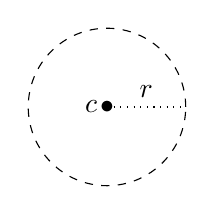
\begin{tikzpicture}[scale=1]
	\draw[dashed] (0,0) circle (1);
	\draw[dotted] (0,0) node {$\bullet$} node[anchor=east] {$c$} -- (1/2,0) node[anchor=south] {$r$} -- (1,0);
\end{tikzpicture}\hspace{3cm}
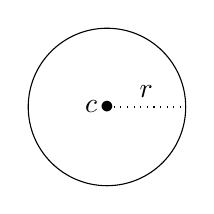
\begin{tikzpicture}[scale=1]
	\draw (0,0) circle (1);
	\draw[dotted] (0,0) node {$\bullet$} node[anchor=east] {$c$} -- (1/2,0) node[anchor=south] {$r$} -- (1,0);
\end{tikzpicture}
\caption{Bolas aberta e fechada de centro $c$ e raio $r$, respectivamente.}
\end{figure}

\begin{prop}
Sejam $\bm M$ um espaço métrico e $C \subseteq M$ um conjunto. Então $C$ é um conjunto limitado se, e somente se, existe bola $\overline\bola_r(c)$ tal que $C \subseteq \overline\bola_r(c)$.
\end{prop}
\begin{proof}
Se $C$ é limitado, basta tomar $r=\diam(C)$ e $c \in C$. Reciprocamente, se existe bola $\overline\bola_r(c)$ tal que $C \subseteq \overline\bola_r(c)$, então para todos $p,p' \in C$, segue da desigualdade triangular que
	\begin{equation*}
	d(p,p') \leq d(p,c)+d(c,p') \leq r+r=2r,
	\end{equation*}
portanto $\diam(C) \leq 2r \in \intfa{0}{\infty}$.
\end{proof}

\begin{defi}
Seja $\bm M$ um espaço métrico. Uma função \emph{limitada} em $\bm M$ é uma função $f\colon X \to M$ de um conjunto $X$ para $M$ cuja imagem $f(X)$ é limitada.
\end{defi}

\section{Topologia dos Espaços Métricos}

\subsection{Interior e Pontos Interiores}

\begin{defi}
Sejam $\bm M$ um espaço métrico e $C \subseteq M$ um conjunto. Um \emph{ponto interior} de $C$ é um ponto $p \in C$ para o qual existe um número real $r > 0$ tal que $\bola_r(p) \subseteq C$. O \emph{interior} de $C$ é o conjunto $\Int{C}$ de todos pontos interiores de $C$. Um \emph{conjunto aberto} de $\bm M$ é um conjunto $A \subseteq M$ tal que $A = A^\circ$. O conjunto dos conjuntos abertos de $\bm M$ é denotado $\topo_{\bm M}$.
\end{defi}

\begin{prop}
Seja $\bm M = (M,d)$ um espaço métrico. Então
	\begin{enumerate}
	\item Para todo $c \in M$ e para todo número real $r > 0$, a bola aberta $\bola_r(c)$ é um conjunto aberto;
	\item O conjunto $\topo_{\bm M}$ é uma topologia de $M$.
	\end{enumerate}
\end{prop}
\begin{proof}
	\begin{enumerate}
	\item Sejam $c \in M$ e $r \in \intaa{0}{\infty}$. Queremos mostrar que $\bola_r(c)$ é aberto. Para isso, seja $p \in \bola_r(c)$. Então segue que $d := d(c,p) < r$, pela definição de bola aberta, e, portanto, $r-d \in \intaa{0}{\infty}$. Para mostrar que essa bola centrada em $p$ está contida na bola maior centrada em $c$, seja $p' \in \bola_{r-d}(p)$. Então $d(p,p')<r-d$ e, pela desigualdade triangular, segue que
	\begin{equation*}
	d(c,p') \leq d(c,p) + d(p,p') < D + (r-d) = r,
	\end{equation*}
o que mostra que $p' \in \bola_r(c)$ e que, portanto, $\bola_s(p) \subseteq \bola_r(c)$. Assim, mostramos que $\bola_r(p)$ é aberta.
	
	\item
		\begin{enumerate}
		\item Podemos notar que $\emptyset$ é aberto por vacuidade, pois, se não fosse, existiria $p \in \emptyset$ para o qual não há $r \in \intaa{0}{\infty}$ satisfazendo $\bola_r(p) \subseteq A$, o que é absurdo.
	Para mostrar que $M$ é aberto, sejam $p \in M$ e $r \in \intaa{0}{\infty}$. Então $\bola_r(p) \subseteq M$, pois qualquer bola aberta é subconjunto de $M$. Portanto $M$ é aberto.
	
		\item Seja $(A_i)_{i \in I}$ uma família de abertos em $\bm M$ e seja $p \in (A_i)_{i \in I}$. Então existe $k \in I$ tal que $p \in A_k$. Como $A_k$ é aberto, então existe $r \in \intaa{0}{\infty}$ tal que $\bola_r(p) \subseteq A_k$. Como $A_k \subseteq (A_i)_{i \in I}$, segue que $\bola_r(p) \subseteq (A_i)_{i \in I}$ e que, portanto, $(A_i)_{i \in I}$ é aberto.
	
		\item Seja $(A_i)_{i \in [n]}$ uma sequência de abertos em $\bm M$ e seja $p \in (A_i)_{i \in [n]}$. Então, para todo $k \in [n]$, $p \in A_k$. Como, para todo $k \in [n]$, $A_k$ é aberto, segue que existe $r_k \in \intaa{0}{\infty}$ tal que $\bola_{r_k}(p) \subseteq A_k$, Seja $r := \min \{r_k : k \in [n]\}$. Então, para todo $k \in [n]$, vale $\bola_r(p) \subseteq \bola_{r_k}(p)$, e segue que $\bola_r(p) \subseteq A_k$ e, portanto, $\bola_r(p) \subseteq (A_i)_{i \in [n]}$, o que mostra que $(A_i)_{i \in [n]}$ é aberto.
		\end{enumerate}		
	\end{enumerate}
\end{proof}

\subsection{Limites e Convergência de Sequências}

\begin{defi}
Sejam $\bm M$ um espaço métrico, $(p_n)_{n \in \N}$ uma sequência de pontos em $M$ e $p \in M$. A sequência $(p_n)_{n \in \N}$  \emph{converge} para o ponto $p$ se, e somente se, para todo número real $\varepsilon > 0$, existe um número natural $N$ tal que
	\begin{equation*}
	\forall n \in \N \qquad n \geq N \Rightarrow p_n \in \bola_\varepsilon(p).
	\end{equation*}
Denota-se $(p_n)_{n \in \N} \conv p$. O ponto $p$ é um \emph{limite} da sequência.  Caso contrário, a sequência não converge para $p$. Uma \emph{sequência convergente} é uma sequência que tem limite. Uma sequência \emph{divergente} é uma sequência que não tem limite.
\end{defi}

\begin{prop}
Todo espaço métrico $\bm M$ é um espaço topológico separado.
\end{prop}
\begin{proof}
Sejam $p,p' \in M$ pontos distintos. Mostraremos que existe um número real $r$ tal que $0 < r \leq \frac{1}{2} d(p,p')$, e que isso implica que $\bola_r(p) \cap \bola_r(p') = \emptyset$. Como $p \neq p'$, então $d(p,p') > 0$, portanto existe $r \in \R$ tal que $0 < r \leq \frac{1}{2} d(p,p')$. Suponhamos que existe $p'' \in \bola_r(p) \cap \bola_r(p')$. Então $d(p,p'')<r$ e $d(p',p'')<r$. Mas, pela desigualdade triangular, segue que
	\begin{equation*}
	d(p,p') \leq d(p,p'') + d(p'',p') < r + r \leq d(p,p'),
	\end{equation*}
o que é absurdo. Portanto $\bola_r(p) \cap \bola_r(p') = \emptyset$.
\end{proof}

\begin{coro}
Toda sequência convergente em um espaço métrico $\bm M$ tem limite único.
\end{coro}
\begin{proof}
Suponhamos que $p,p'$ são limites de $(p_n)_{n \in \N}$. Se $p \neq p'$, então $d(p,p')>0$. Seja $\varepsilon \in \R$ tal que $0 < \varepsilon \leq \frac{1}{2} d(p,p')$. Então existe $N_1 \in \N$ tal que, para todo $n \in \N$, se $n \geq N_1$, então $p_n \in \bola_\varepsilon(p)$, e existe $N_2 \in \N$ tal que, para todo $n \in \N$, se $n \geq N_2$, então $p_n \in \bola_\varepsilon(p')$. Assim, definindo $N := \max \{N_1,N_2\}$, segue que, se $n \geq N$, então $n \geq N_1$ e $n \geq N_2$, e, portanto, que $p_n \in \bola_\varepsilon(p)$ e $p_n \in \bola_\varepsilon(p')$; ou seja, $p_n \in \bola_\varepsilon(p) \cap \bola_\varepsilon(p')$, mas isso é absurdo, pois $\bola_\varepsilon(p) \cap \bola_\varepsilon(p')=\emptyset$. Portanto $p=p'$.
\end{proof}

Essa proposição nos permite tratar o limite de uma sequência como um número único e, por isso, podemos usar a notação $\displaystyle\lim_{n \in \N} p_n = p$ para quando $(p_n)_{n \in \N} \conv p$.

\begin{prop}
Uma sequência de em um espaço métrico $\bm M$ é convergente se, e somente se, todas suas subsequências são convergentes.
\end{prop}
\begin{proof}
	Suponhamos que $(p_n) \conv p$ e seja $(p_{n_k})_{k \in \N}$ uma subsequência de $(p_n)_{n \in \N}$. Seja $\varepsilon \in \R$ tal que $\varepsilon > 0$. Como $(p_n) \conv p$, existe $N \in \N$ tal que, para todo $n \in \N$, se $n \geq N$, então $p_n \in \bola_\varepsilon(p)$; como $(n_k)_{k \in \N}$ é estritamente crescente, existe $K \in \N$ tal que, para todo $k \in \N$, se $k \geq K$, então $n_k \geq N$. Mas então
	\begin{equation*}
	k \geq K \Rightarrow n_k \geq N \Rightarrow p_{n_k} \in \bola_\varepsilon(p)
	\end{equation*}
e, portanto, $(p_{n_k}) \to p$.	Reciprocamente, se toda subsequência de $(p_n)_{n \in \N}$ converge para $p$, $(p_n)_{n \in \N}$, em particular, é uma dessas subsequências e, portanto, $(p_n) \conv p$.
\end{proof}

\begin{prop}
Toda sequência convergente em um espaço métrico $\bm M$ é limitada.
\end{prop}
\begin{proof}
	Seja $(p_n)_{n \in \N}$ uma sequência de pontos em $M$ tal que $(p_n) \conv p$. Então, para $\varepsilon = 1$, existe $N \in \N$ tal que, para todo $n \in \N$, se $n \geq N$, então $p_n \in \bola_1(p)$. Assim, seja $l \in \R$ tal que
	\begin{equation*}
	l > \max(\{1\} \cup \{d(p,p_n) : n \in [N]\}),
	\end{equation*}
seque que, para todo $n \in \N$, $p_n \in \bola_l(p)$ pois, se $0 \leq n \leq N$, $d(p,p_n) < l$ pela definição de $l$ e, se $n \geq N$, então $p_n \in \bola_1(p) \subseteq B_l(p)$, pois $1 < l$. Logo $(p_n)_{n \in \N}$ é limitada.
\end{proof}

\begin{prop}
Sejam $\bm M$ um espaço métrico, $C \subseteq M$ um conjunto e $p \in M$. Então existe uma sequência de pontos em $C$ que converge para $p$ se, e somente se, para todo número real $\varepsilon > 0$, $C \cap \bola_\varepsilon(p) \neq \emptyset$.
\end{prop}
\begin{proof}
	Suponhamos que exista uma sequência $(p_n)_{n \in \N}$ de pontos em $C$ tal que $(p_n) \conv p$. Então, para todo número real $\varepsilon > 0$, existe $N \in \N$ tal que, para todo $n \in \N$, se $n \geq N$, então $p_n \in \bola_\varepsilon(p)$. Mas isso implica que $p_n \in C \cap \bola_\varepsilon(p)$. Reciprocamente, suponhamos que, para todo número real $\varepsilon > 0$, $C \cap \bola_\varepsilon(p) \neq \emptyset$. Então, em particular, para todo $n \in \N$, escolhamos $p_n \in C \cap \bola_{\frac{1}{n}}(p)$. Assim, temos a sequência $(p_n)_{n \in \N}$. Para mostrar que $(p_n) \conv p$, seja $\varepsilon \in \R$ tal que $\varepsilon > 0$. Então existe $N \in \N$ tal que $\frac{1}{N} \leq \varepsilon$. Mas isso implica que, para todo número natural $n \geq N$, $\frac{1}{n} \leq \frac{1}{N}$, e segue que
	\begin{equation*}
	d(p,p_n) < \frac{1}{n} \leq \frac{1}{N} \leq \varepsilon
	\end{equation*}
e, portanto, $(p_n) \conv p$.
\end{proof}

\begin{prop}
Sejam $\bm M$ um espaço métrico, $p,q \in M$ e $(p_n)_{n \in \N}$ e $(q_n)_{n \in \N}$ sequências em $M$ que convergem para $p$ e $q$ respectivamente. Então a sequência $(d(p_n,q_n))_{n \in \N}$ em $\R$ converge para $d(p,q)$.
\end{prop}
\begin{proof}
	Para todo $n \in \N$, segue da desigualdade triangular que
	\begin{equation*}
	d(p_n,q_n) \leq d(p_n,p) + d(p,q) + d(q,q_n).
	\end{equation*}
Seja $\varepsilon > 0$ um número real. Então existem $N_1,_2 \in \N$ tais que
	\begin{equation*}
	\forall n \in \N \qquad n \geq N_1 \Rightarrow d(p,p_n) < \frac{\varepsilon}{2}
	\end{equation*}
e
	\begin{equation*}
	\forall n \in \N \qquad n \geq N_2 \Rightarrow d(q,q_n) < \frac{\varepsilon}{2}.
	\end{equation*}
Fazendo $N_3 := \max\{N_1,N_2\}$, segue que
	\begin{equation*}
	\forall n \in \N \qquad n \geq N_3 \Rightarrow d(p_n,q_n) \leq d(p_n,p) + d(p,q) + d(q,q_n) < d(p,q) + \varepsilon;
	\end{equation*}
ou seja, $d(p_n,q_n) - d(p,q) < \varepsilon$. Analogamente, achamos $N_6 \in \N$ tal que
	\begin{equation*}
	\forall n \in \N \qquad n \geq N_3 \Rightarrow d(p_n,q_n) \leq d(p_n,p) + d(p,q) + d(q,q_n) < d(p,q) + \varepsilon
	\end{equation*}
e fazendo $n := \max\{N_3,N_6\}$, segue que
	\begin{equation*}
	\forall n \in \N \qquad n \geq N \Rightarrow |d(p,q) - d(p_n,q_n)| < \varepsilon,
	\end{equation*}
o que mostra que $(d(p_n,q_n)) \conv d(p,q)$ em $\R$.
	
\end{proof}

\subsection{Fecho e Pontos Aderentes}

\begin{defi}
Sejam $\bm M$ um espaço métrico e $C \subseteq M$ um conjunto. Um \emph{ponto aderente} a $C$ é um ponto $p \in M$ para o qual existe uma sequência $(p_n)_{n \in \N}$ de pontos de $C$ que converge para $p$. O \emph{fecho} de $C$ é o conjunto $\Fec{C}$ de todos os pontos aderentes a $C$. Um \emph{conjunto fechado} de $\bm M$ é um conjunto $F \subseteq M$ tal que $F = \Fec{F}$.
\end{defi}

\begin{prop}
Sejam $\bm M$ um espaço métrico e $F \subseteq M$. Então $F$ é um conjunto fechado se, e somente se, $F^\complement$ é um conjunto aberto.
\end{prop}
\begin{proof}
Suponhamos que $F$ é um conjunto fechado. Se $F^\complement = \emptyset$, Mas $\emptyset$ é aberto pois, caso contrário, existe $p \in \emptyset$ para o qual não há número real $\varepsilon > 0$ tal que $\bola_\varepsilon(p) \subseteq \emptyset$, mas isso é absurdo. Se $F^\complement \neq \emptyset$, seja $p \in F^\complement$. Se não existe número real $\varepsilon > 0$ tal que $\bola_\varepsilon(p) \subseteq F^\complement$, então, para todo número real $\varepsilon > 0$, $F \cap \bola_\varepsilon(p) \neq \emptyset$. Mas isso implica que existe uma sequência $(p_n)_{n \in \N}$ de pontos em $F$ tal que $(p_n) \conv p$. Como $F$ é fechado, isso implica $p \in F$, o que é uma contradição. Então existe número real $\varepsilon > 0$ tal que $\bola_\varepsilon(p) \subseteq F^\complement$, e isso mostra que $F^\complement$ é aberto.
	
Reciprocamente, suponhamos que $F^\complement$ é aberto. Se $F = \emptyset$, então $F$ é fechado. Se $F \neq \emptyset$, seja $(p_n)_{n \in \N}$ uma sequência em $F$ que converge para $p \in M$. Suponhamos que $p \notin F$. Então $p \in F^\complement$ e, como $F^\complement$ é aberto, existe um número real $\varepsilon > 0$ tal que $\bola_\varepsilon(p) \subseteq F^\complement$. Como $(p_n) \conv p$, existe $N \in \N$ tal que, para todo $n \in \N$, se $n \geq N$, então $p_n \in \bola_\varepsilon(p)$. Mas isso implica que $p_N \in \bola_\varepsilon(p) \subseteq F^\complement$, o que é absurdo, pois $p_n \in F$. Portanto $p \in F$ e isso mostra que $F$ é fechado.
\end{proof}

\begin{prop}
Seja $\bm M$ um espaço métrico. Então, para todo $c \in M$ e para todo número real $r > 0$, a bola fechada $\bar\bola_r(c)$ é um conjunto fechado.
\end{prop}
\begin{proof}
Basta notar que $\bar\bola_r(c)^\complement$ é aberto.
\end{proof}

\subsection{Conjuntos Densos}

\begin{defi}
	Sejam $\bm M$ um espaço métrico e $C \subseteq M$ um conjunto. Um conjunto \emph{denso em $C$} é um conjunto $D \subseteq M$ tal que $C \subseteq \overline D$.
\end{defi}

	Isso que dizer que, para todo ponto de $C$, existe uma sequência em $D$ que converge para esse ponto.
	
\begin{prop}
	Sejam $\bm M = (M,d)$ um espaço métrico e $C,D \subseteq M$ conjuntos. Então $D$ é denso em $C$ se, e somente se, para todo conjunto aberto $A$ de $\bm M$, $A \cap C \neq \emptyset$ implica $A \cap D \neq \emptyset$.
\end{prop}
\begin{proof}
	Suponhamos que $D$ é denso em $C$. Sejam $A$ um conjunto aberto de $\bm M$ tal que $A \cap C \neq \emptyset$ e seja $p \in A \cap C$. Como $D$ é denso em $C$ e $p \in C$, existe uma sequência $(p_n)_{n \in \N}$ em $D$ que converge para $p$. Como $A$ é aberto e $p \in A$, existe um número real $\varepsilon>0$ tal que $\bola_\varepsilon(p) \subseteq A$. Então, como $(p_n) \conv p$, existe um número natural $N$ tal que, para todo natural $n \geq N$, $p_n \in \bola_\varepsilon(p)$. Mas isso implica que $p_n \in A \cap D$.
	
	Reciprocamente, suponhamos que, para todo conjunto aberto $A$ de $\bm M$, $A \cap C \neq \emptyset$ implica $A \cap D \neq \emptyset$. Se $C=\emptyset$, então $C \subseteq \overline D$. Se $C \neq \emptyset$, seja $p \in C$. Para todo $n \in \N$, o conjunto $\bola_\frac{1}{n}(p)$ é um conjunto aberto que contém $p$. Mas então $\bola_\frac{1}{n}(p) \cap C \neq \emptyset$, o que implica $\bola_\frac{1}{n}(p) \cap D \neq \emptyset$. Para cada $n \in \N$, escolhamos $p_n \in B_\frac{1}{n}(p) \cap D$. Assim, temos uma sequência $(p_n)_{n \in \N}$ de pontos em $D$ que converge para $p$, pois, para todo número real $\varepsilon>0$, existe um natural $N$ tal que $\frac{1}{N} \leq \varepsilon$ e, então
	\begin{equation*}
	\forall n \in \N \qquad n \geq N \Rightarrow \frac{1}{n} \leq \frac{1}{N} \leq \varepsilon \Rightarrow p_n \in \bola_\frac{1}{n}(p) \subseteq \bola_\frac{1}{N}(p) \subseteq \bola_\varepsilon(p).
	\end{equation*}
	Isso mostra que $p \in \overline D$ e, portanto, que $C \subseteq \overline D$.
\end{proof}

\begin{prop}
	Sejam $\bm M_1$ e $\bm M_2$ espaços métricos e $f,g\colon M_1 \to M_2$ funções contínuas. Então o conjunto 
	\begin{equation*}
	F := \set{p \in M_1}{f(p)=g(p)}
	\end{equation*}
é um conjunto fechado.
\end{prop}
\begin{proof}
	Se $F=\emptyset$, então $F$ é fechado. Se $F \neq \emptyset$, seja $(p_n)_{n \in \N}$ uma sequência em $F$ que converge para $p \in M_1$. Mostraremos que $p \in F$. Como $f$ e $g$ são contínuas em $p$, segue que
	\begin{equation*}
	(f(p_n)) \conv f(p) \e (g(p_n)) \conv g(p).
	\end{equation*}
	Como $(p_n)_{n \in \N}$ é uma sequência em $F$, as sequências $(f(p_n))_{n \in \N}$ e $(g(p_n))_{n \in \N}$ são a mesma sequência e segue da unicidade do limite que $f(p)=g(p)$, o que mostra que $p \in F$ e que, portanto, $F$ é um conjunto fechado.
\end{proof}

\begin{prop}
	Sejam $\bm M_1$ e $\bm M_2$ espaços métricos, $f,g: M_1 \to M_2$ funções contínuas e $C,D \subseteq M_1$ conjuntos tais que $D$ é denso em $C$. Se $f|_D = g|_D$, então $f|_C = g|_C$.
\end{prop}
\begin{proof}
	Pela proposição anterior, sabemos que $F := \{p \in M_1 : f(p)=g(p)\}$ é um conjunto fechado. Como $f|_D = g|_D$, então $D \subseteq F$. Mas isso significa que $\overline D \subseteq \overline F = F$ e, como $D$ é denso em $C$, segue que $C \subseteq \overline D \subseteq F$ e, portanto, que $f|_C = g|_C$. 
\end{proof}

\subsection{Conjuntos Compactos}

\begin{prop}
Sejam $\bm M$ um espaço métrico e $C \subseteq M$. Se $C$ é compacto, então é limitado.
\end{prop}
\begin{proof}
Seja $p \in M$ e consideremos a cobertura $\set{\bola_r(p)}{r \in \intaa{0}{\infty}}$ de $C$. Pela compacidade, existe subcobertura finita $\{\bola_{r_0}(p),\ldots,\bola_{r_{n-1}}(p)\}$ de $C$. Tomando $r := \max\set{r_i}{i \in [n]}$, segue que $\bola_{r_i}(p) \subseteq \bola_{r}(p)$ para todo $i \in [n]$, logo $C \subseteq \bola_r(p)$, o que implica que $\diam(C) \leq 2r < \infty$. 
\end{proof}

A recíproca nem sempre é verdade. Nos espaços $\R^d$, $ d \in \N$, vale que um conjunto é compacto se, e somente se, é fechado e limitado. Esse resultado é conhecido como Teorema de Heine-Borel. No entanto, isso não vale em qualquer espaço métrico\footnote{Para mais detalhes, conferir \url{https://math.stackexchange.com/questions/674982/difference-between-closed-bounded-and-compact-sets}.}.

\subsection{Continuidade}

\begin{defi}
Sejam $\bm M$ e $\bm M'$ espaços métricos e $p \in M$. Uma função \emph{contínua em $p$} é uma função $f\colon M \to M'$ que satisfaz: para todo $\varepsilon \in \intaa{0}{\infty}$, existe $\delta \intaa{0}{\infty}$ tal que, para todo $x \in M$
%	\begin{equation*}
%	\qquad d_1(p,x) < \delta \Rightarrow d_2(f(p),f(x)) < \varepsilon.
%	\end{equation*}
	\begin{equation*}
	x \in \bola_\delta(p) \Rightarrow f(x) \in \bola_\varepsilon(f(p)).
	\end{equation*}
Uma função \emph{descontínua} em $p$ é uma função que não é contínua em $p$.
\end{defi}

Denotamos as bolas abertas em $\bm M$ e em $\bm M'$ por $\bola$, mas deve-se perceber que elas são relativas a métricas possivelmente diferentes.

\begin{prop}
Sejam $\bm M_1$ e $\bm M_2$ espaços métricos, $f: M_1 \to M_2$ uma função e $p \in M_1$. Então $f$ é contínua em $p$ se, e somente se, para toda sequência $(p_n)_{n \in \N}$ de pontos em $M_1$ que converge para $p$, a sequência $(f(p_n))_{n \in \N}$ de pontos em $M_2$ converge para $f(p)$; ou seja
	\begin{equation*}
	\lim f(p_n) = f(\lim p_n).
	\end{equation*}
\end{prop}
\begin{proof}
	Suponhamos que $f$ é contínua em $p$. Seja $(p_n)_{n \in \N}$ uma sequência de pontos em $M_1$ que converge para $p$. Seja um número real $\varepsilon > 0$. Como $f$ é contínua, existe um número real $\delta > 0$ tal que $p_n \in \bola_\delta(p)$ implica $f(p_n) \in \bola_\varepsilon(f(p))$. Mas, como $(p_n) \conv p$, existe $N \in \N$ tal que
	\begin{equation*}
	\forall n \in \N \qquad n \geq N \Rightarrow p_n \in \bola_\delta(p) \Rightarrow f(p_n) \in \bola_\varepsilon(f(p))
	\end{equation*}
o que mostra que $(f(p_n)) \conv f(p)$.
	
	Reciprocamente, suponhamos que, para toda sequência $(p_n)_{n \in \N}$ em $M_1$ que converge para $p$, a sequência $(f(p_n))_{n \in \N}$ converge para $f(p)$. Suponhamos, por absurdo, que $f$ não é contínua em $p$. Então existe um número real $\varepsilon > 0$ tal que, para todo número real $\delta > 0$, existe $x \in M_1$ tal que $x \in \bola_\delta(p)$, mas $f(x) \notin \bola_\varepsilon(f(p))$. Vamos mostrar que isso implica que existe uma sequência $(p_n)_{n \in \N}$ em $M_1$ que converge para $p$, mas que a sequência $(f(p_n))_{n \in \N}$ não converge para $f(p)$; ou seja, que existe um número real $\varepsilon > 0$ tal que, para todo número natural $N$, existe $n \in \N$ tal que $n \geq N$, mas $f(p_n) \notin \bola_\varepsilon(f(p))$. Seja $n \in \N$ e tomemos $\delta = \frac{1}{n}$. Então existe $x \in M_1$ tal que $x \in \bola_\frac{1}{n}(p)$, mas $f(x) \notin \bola_\varepsilon(f(p))$. Nomeando esse $x \in M_1$ de $p_n$, obtemos uma sequência $(p_n)_{n \in \N}$ que converge para $p$ pois, para todo número real $\varepsilon' > 0$, existe um número natural $N \in \N$ tal que $\frac{1}{N} \leq \varepsilon'$ e isso implica que
\begin{equation*}
	\forall n \in \N \qquad n \geq N \Rightarrow \frac{1}{n} \leq \frac{1}{N} \leq \varepsilon' \Rightarrow p_n \in \bola_\frac{1}{n}(p) \subseteq \bola_\frac{1}{N}(p) \subseteq \bola_{\varepsilon'}(p).
	\end{equation*}
	No entanto, $(f(p_n))_{n \in \N}$ é uma sequência que não converge para $f(p)$ pois, considerando o $\varepsilon$ original tomado da descontinuidade de $f$, para todo número natural $N$, $f(p_N) \notin \bola_\varepsilon(f(p))$ e isso contradiz a hipótese de que, para toda sequência $(p_n)_{n \in \N}$ em $M_1$ que converge para $p$, a sequência $(f(p_n))_{n \in \N}$ converge para $f(p)$. Portanto $f$ é contínua.	
\end{proof}

\begin{defi}
Sejam $\bm M_1$ e $\bm M_2$ espaços métricos, $D \subseteq M_1$ e $f: D \to M_2$ uma função. A função $f$ é \emph{contínua} em $D$ se ela é contínua em todo ponto de $D$. Caso contrário, a função $f$ é \emph{descontínua} em $D$. Para $D=M_1$, dizemos simplesmente que $f$ é contínua ou descontínua.
\end{defi}

\subsection{Ponto Limite e Conjunto Derivado}

\begin{defi}
Sejam $\bm M$ um espaço métrico e $C \subseteq M$ um conjunto. Um \emph{ponto limite} (ou \emph{ponto de acumulação}) de $C$ é um ponto $p \in M$ para o qual existe uma sequência $(p_n)_{n \in \N}$ de pontos de $C \setminus \{p\}$ que converge para $p$. O \emph{derivado} de $C$ é o conjunto de todos os pontos limites de $C$. 
\end{defi}

Da definição, segue que $C' \subseteq \overline C$. A inclusão contrária caracteriza a seção a seguir.

\begin{defi}
Sejam $\bm M$ um espaço métrico e $C \subseteq M$ um conjunto. Um \emph{ponto isolado} de $C$ é um ponto $p \in M$ que é um ponto aderente a $C$ mas que não é um ponto limite de $C$.
\end{defi}

Um ponto isolado de $C$ é um ponto $p \in \overline C \setminus C'$.

\subsection{Separação Métrica}

\begin{defi}
Seja $\bm M$ um espaço métrico. Conjuntos \emph{metricamente separados} de $\bm M$ são conjuntos $C,C' \subseteq M$ tais que
	\begin{equation*}
	\dist{C}{C'} > 0.
	\end{equation*}
\end{defi}

\section{Estrutura Uniforme}

\subsection{Sequências Aproximantes}

\begin{defi}
Seja $\bm M$ um espaço métrico. Uma sequência \emph{aproximante} em $\bm M$ é uma sequência $(p_n)_{n \in \N}$ de pontos em $M$ tal que, para todo número real $\varepsilon > 0$, existe um número natural $N$ satisfazendo
	\begin{equation*}
	\forall n,m \in \N \qquad n,m \geq N \Rightarrow d(p_n,p_m) < \varepsilon.
	\end{equation*}
\end{defi}

Essa sequências são conhecidas como \emph{sequências de Cauchy}. O nome aproximante se dá pelo fato de que os termos da sequência ficam cada vez mais próximos entre si, e será adotado por ser mais intuitivo, embora não seja a nomenclatura padrão.

\begin{prop}
Toda sequência convergente em um espaço métrico $\bm M$ é aproximante.
\end{prop}
\begin{proof}
Seja $(p_n)_{n \in \N}$ uma sequência em $M$ que converge para $p$. Seja $\varepsilon \in \R$ tal que $\varepsilon > 0$. Então $\frac{1}{2}\varepsilon > 0$ é um número real e segue que existe $N \in \N$ tal que, para todo número natural $n \geq N$, $p_n \in \bola_{\frac{1}{2}\varepsilon}(p)$. Assim, segue que	
	\begin{equation*}
	\forall n,m \in \N \qquad n,m \geq N \Rightarrow d(p_n,p_m) \leq d(p_n,p) + d(p,p_m) < \frac{\varepsilon}{2} + \frac{\varepsilon}{2} = \varepsilon,
	\end{equation*}
o que mostra que $(p_n)_{n \in \N}$ é uma sequência aproximante.
\end{proof}

\begin{prop}
Toda sequência aproximante em um espaço métrico $\bm M$ que tem uma subsequência convergente é convergente.
\end{prop}
\begin{proof}
	Seja $(p_{n_k})_{k \in \N}$ uma subsequência de $(p_n)_{n \in \N}$ que converge  para $p$. Seja $\varepsilon > 0$ um número real. Como $(p_n)_{n \in \N}$ é uma sequência de Cauchy e $\frac{1}{2}\varepsilon > 0$ é um número real, existe um número natural $N$ tal que
	\begin{equation*}
	\forall n,m \in \N \qquad n,m \geq N \Rightarrow d(p_n,p_m) < \frac{\varepsilon}{2}.
	\end{equation*}
Como $(p_{n_k})_{k \in \N}$ é uma subsequência convergente, existe $K_1 \in \N$ tal que
	\begin{equation*}
	\forall k \in \N \qquad k \geq K_1 \Rightarrow d(p,p_{n_k}) < \frac{\varepsilon}{2}.
	\end{equation*}
Como $(n_k)_{k \in \N}$ é uma sequência estritamente crescente, existe $K_2 \in \N$ tal que, para todo número natural $k \geq K_2$, $n_k \geq N$. Assim, tomando $K := \max\{K_1,K_2\}$, segue que, para todo número natural $n \in \N$, existe $k \in \N$ tal que $n_k \geq N$ e,  pela desigualdade triangular, que
	\begin{equation*}
	\forall n \in \N \qquad n \geq N \Rightarrow d(p_n,p) \leq d(p_n,p_{n_k}) + d(p_{n_k},p) < \frac{\varepsilon}{2}+\frac{\varepsilon}{2}=\varepsilon.
	\end{equation*}
\end{proof}

\begin{prop}
Toda sequência aproximante em um espaço métrico $\bm M$ é limitada.
\end{prop}
\begin{proof}
Seja $(p_n)_{n \in \N}$ uma sequência aproximante em $\bm M$. Então, para $\varepsilon=1$, existe $N \in \N$ tal que
	\begin{equation*}
	\forall n,m \in \N \qquad n,m \geq N \Rightarrow d(p_n,p_m)<1.
	\end{equation*}
	Definamos $P := \{p_n : n \in \N\}$. Então segue que
	\begin{align*}
	\diam(P) &= \sup \set{d(p_n,p_m)}{n,m \in \N} \\
		&= \max\{1 \cup \set{d(p_n,p_m)}{0 \leq n,m \leq N}\} \in \R,
	\end{align*}
o que mostra que $(p_n)_{n \in \N}$ é limitada.
\end{proof}

\subsection{Continuidade Uniforme}

\begin{defi}
Sejam $\bm M_1$ e $\bm M_2$ espaços métricos. Uma função \emph{uniformemente contínua} é uma função $f: M_1 \to M_2$ tal que, para todo número real $\varepsilon > 0$, existe um número real $\delta > 0$ tal que
	\begin{equation*}
	\forall p_1,p_2 \in M_1 \qquad d_1(p_1,p_2) < \delta \Rightarrow d_2(f(p_1),f(p_2)) < \varepsilon.
	\end{equation*}
\end{defi}

\begin{prop}
Sejam $\bm M_1$ e $\bm M_2$ espaços métricos, $f: M_1 \to M_2$ uma função uniformemente contínua e $(p_n)_{n \in \N}$ uma sequência aproximante em $M_1$. Então a sequência $(f(p_n))_{n \in \N}$ em $M_2$ é aproximante.
\end{prop}
\begin{proof}
Seja $\varepsilon > 0$ um número real. Da continuidade uniforme de $f$, existe um número real $\delta > 0$ tal que, para todo $p,p' \in M_1$, $d_1(p,p') < \delta$ implica $d_2(f(p),f(p')) < \varepsilon$. Como $(p_n)_{n \in \N}$ é sequência aproximante, existe $N \in \N$ tal que
	\begin{equation*}
	\forall n,m \in \N \qquad n,m \geq N \Rightarrow d_1(p_n,p_m) < \delta.
	\end{equation*}
Mas, da continuidade uniforme de $f$, isso implica que
	\begin{equation*}
	\forall n,m \in \N \qquad n,m \geq N \Rightarrow d_1(p_n,p_m) < \delta  \Rightarrow d_2(f(p_n),f(p_m)) < \varepsilon,
	\end{equation*}
e isso mostra que $(f(p_n))_{n \in \N}$ é uma sequênca aproximante.
\end{proof}

\subsection{Espaços Métricos Completos}

\begin{defi}
Um espaço métrico \emph{completo} é um espaço métrico em que todas sequências aproximantes convergem.
\end{defi}

\begin{prop}
Seja $\bm M$ um espaço métrico. Todo subespaço completo de $\bm M$ é um conjunto fechado em $\bm M$.
\end{prop}
\begin{proof}
Sejam $\bm C \subseteq \bm M$ subsepaço métrico completo e $(p_n)_{n \in \N}$ uma sequência convergente em $C$. Então $(p_n)_{n \in \N}$ é aproximante e, como $C$ é completo, converge para um ponto em $C$, o que significa que $C$ é fechado.
\end{proof}

\begin{prop}
Sejam $\bm M$ um espaço métrico, $\bm C \subseteq \bm M$ um subespaço completo e $F \subseteq C$ um conjunto fechado em $\bm M$. Então $\bm F$ é completo.
\end{prop}
\begin{proof}
Seja $(p_n)_{n \in \N}$ uma sequência aproximante em $F$. Então $(p_n)_{n \in \N}$ é uma sequência aproximante em $C$ e, como $C$ é completo, $(p_n)_{n \in \N}$ converge. Porém, como $F$ é fechado, então $(p_n)_{n \in \N}$ converge para um ponto em $F$, o que mostra que $F$ é completo.
\end{proof}

\begin{teo}
Seja $\bm M$ um espaço métrico. Então $\bm M$ é completo se, e somente se, para toda sequência descrescente $(F_n)_{n \in \N}$ de conjuntos não vazios e fechados em $\bm M$ tais que $(\diam(F_n))_{n \in \N} \conv 0$ em $\R$, vale que
	\begin{equation*}
	\bigcap_{n \in \N} A_n \neq \emptyset.
	\end{equation*}
\end{teo}

\begin{teo}
Sejam $\bm M_1$  um espaço métrico, $\bm M_2$ espaço métrico completo, $D \subseteq M_1$ um conjunto denso em $M_1$ e $f: D \to M_2$ uma função uniformemente contínua. Então $f$ tem uma única extensão para uma função uniformemente contínua $f^*: M_1 \to M_2$. Ainda, se $f$ é uma isometria, então $f^*$ é uma isometria.
\end{teo}
\begin{proof}
	Seja $p \in M_1$. Como $D$ é denso em $M_1$, existe uma sequência $(p_n)_{n \in \N}$ em $D$ que converge para $p$. Como $(p_n)_{n \in \N}$ é convergente, é uma sequência de Cauchy e, como $f$ é uniformemente contínua em $D$, segue que $(f(p_n))_{n \in \N}$ é uma sequência de Cauchy em $M_2$. Mas $M_2$ é completo, o que implica que $(f(p_n))_{n \in \N}$ converge para um ponto $p' \in M_2$. Definimos, portanto, a função $f^*$ em $p$ como $f^*(p)=p'$. Precisamos mostrar que $f^*$ independe da escolha da sequência em $D$ que converge para $p$. Se $(q_n)_{n \in \N}$ é uma sequência em $D$ que converge para $p$, definamos a sequência $(r_n)_{n \in \N}$ em $D$ por
	\begin{equation*}
	r_n :=
			\begin{cases}
			p_n &\text{se $n=2k$}\\
			q_n &\text{se $n=2k+1$}.
			\end{cases}
	\end{equation*}
A sequência $(r_n)_{n \in \N}$ converge para $p$ e, portanto, é uma sequência de Cauchy. A continuidade uniforme de $f$ implica que a sequência $(f(r_n))_{n \in \N}$ é de Cauchy e, portanto, como $(f(p_n))_{n \in \N}=(f(r_{2k}))_{k \in \N}$ é uma subsequência que converge para $p'$, a sequência $(f(r_n))_{n \in \N}$ converge para $p'$, o que implica que a subsequência $(f(q_n))_{n \in \N}=(f(r_{2k+1}))_{k \in \N}$ converge para $p'$. Assim, mostramos que $f^*$ está bem definida. Claramente, se $p \in D$, então $f(p)=f^*(p)$, pois, como $D$ é denso em $M_1$, se $(p_n)_{n \in \N}$ é uma sequência em $D$ que converge para $p$, então, como $f$ é contínua, segue que $f(p_n) \conv f(p)$, o que mostra que $f^*(p)=f(p)$.

	Agora, devemos mostrar que $f^*$ é uniformemente contínua. Seja $\varepsilon > 0$ um número real, então $\frac{1}{2}\varepsilon > 0$ é um número real e, como $f$ é uniformemente contínua, existe número real $\delta > 0$ tal que
	\begin{equation*}
	\forall p,p' \in M_1 \qquad d_1(p,p') < \delta \Rightarrow d_2(f(p),f(p')) < \frac{\varepsilon}{2}.
	\end{equation*}
Assim, sejam $p,q \in M_1$ tais que $d_1(p,q) < \delta$. Quremos mostrar que $d_2(f(p),f(p')) < \varepsilon$. Sejam $(p_n)_{n \in \N}$ e $(q_n)_{n \in \N}$ sequências que convergem para $p$ e $q$, respectivamente. Então $d_1(p_n,q_n) \conv d_1(p,q)$ em $\R$.

...

	A unicidade de $f^*$ ocorre pois, se existem $f^*$ e $f'^*$ uniformemente contínuas que extendem $f$, como $D$ é denso em $M_1$ e $f^*|_D = f'^*|_D$, segue que $f^* = f'^*$ .
	
	Por fim, mostramos que a isometria se preserva...
\end{proof}

\begin{defi}
Seja $\bm M_1$  um espaço métrico. Um \emph{completamento} de $\bm M$ é um espaço métrico $\bm M_2$ completo tal que $M_1$ é denso em $M_2$.
\end{defi}

\begin{prop}
Seja $\bm M$ um espaço métrico e $\bm M_1$ e $\bm M_2$ completamentos de $\bm M$. Então existe uma isometria entre $\bm M_1$ e $\bm M_2$ que é a função identidade quando restrita a $M$.
\end{prop}
\begin{proof}
	Seja $f$ a função identidade em $M$. Pela proposição anterior, existe uma única extensãouniformemente contínua de $f^*$ em $M_1$ ...
	
	...
\end{proof}


\begin{prop}
Sejam $K \subseteq M$ compacto e $f: M \to \bar M$ contínua. Então $f$ é uniformemente contínua.
\end{prop}
\begin{proof}
Suponhamos, por absurdo, que $f$ não é uniformemente contínua. Então existem $\varepsilon > 0$ e $(x_n)_{n \in \N},(y_n)_{n \in \N}$ sequências em $K$ tais que
	\begin{equation*}
	\nor{x_n - y_n} < \frac{1}{n} \e \nor{f(x_n)-f(y_n)} \geq \varepsilon.
	\end{equation*}
Como $K$ é compacto, existem subsequências $(x_{n_k})_{k \in \N}$  e $(y_{n_k})_{k \in \N}$ convergindo a $x \in K$ com $\nor{f(x_{n_k})-f(y_{n_k})} \geq \varepsilon$. Por continuidade de $f$, existe $\delta > 0$ tal que, se $x_{n_k},y_{n_k} \in B(x,\delta)$, então $\nor{f(x_{n_k})-f(x)} < \frac{\varepsilon}{2}$ e $\nor{f(y_{n_k})-f(x)} < \frac{\varepsilon}{2}$. Pela desigualdade triangular, temos um absudo.
\end{proof}

\section{Funções que Preservam Distância}

\subsection{Funções Métricas (ou Subsemelhanças)}

\begin{defi}
Sejam $\bm M_0$ e $\bm M_1$ espaços métricos e $c \in \intfa{0}{\infty}$. Uma função \emph{métrica}\footnote{Essas funções são conhecidas geralmente como funções `Lipschitz' contínuas.} de $\bm M_0$ para $\bm M_1$ (com constante $c$) é uma função $f\colon M_0 \to M_1$ que satisfaz, para todos $p,p' \in M_0$,
	\begin{equation*}
	d_1(f(p),f(p')) \leq cd_0(p,p').
	\end{equation*}
Para $0 \leq c < 1$, a função $f$ é uma \emph{contração}; para $c=1$, é uma \emph{homometria}\footnote{Essas funções são também conhecidas como funções métricas, funções não expansoras, entre outros. Escolhi o nome homometria por uma relação que elas têm com as isometrias que serão definidas mais à frente}.
\end{defi}

\begin{prop}
Sejam $\bm M_0, \bm M_1$ e $\bm M_2$ espaços métricos, $f_0\colon M_0 \to M_1$ uma função métrica (com constante $c_0$) e $f_1\colon M_1 \to M_2$ uma função métrica (com constante $c_1$). Então $f_1 \circ f_0\colon M_0 \to M_2$ é uma função métrica (com constante $c_1c_0$). Se $f_0$ e $f_1$ são contrações, $f_1 \circ f_0$ é uma contração, e se $f_0$ e $f_1$ são funções métricas, então $f_1 \circ f_0$ é uma função métrica.
\end{prop}
\begin{proof}
Para todos $p,p' \in M_0$,
	\begin{equation*}
	d_2(f_1 \circ f_0(p),f_1 \circ f_0(p')) \leq c_1d_2(f_0(p),f_0(p')) \leq c_1c_0d_0(p,p').
	\end{equation*}
Claramente, se $0 \leq c_0 < 1$ e $0 \leq c_1 < 1$, então $0 \leq c_1c_0 < 1$, e se $c_0=c_1=1$, então $c_1c_0=1$.
\end{proof}

\begin{prop}
Sejam $\bm M_0$ e $\bm M_1$ espaços métricos e $f\colon M_0 \to M_1$ uma função métrica (com constante $c$). Então $f$ é uniformemente contínua.
\end{prop}
\begin{proof}
Se $c=0$, a demonstração é óbvia. Se $c \neq 0$, seja $\varepsilon>0$. Tomando $\delta=\frac{\varepsilon}{c}$, segue que, para todos $p,p' \in M_0$, se $d_0(p,p') \leq \delta$, então
	\begin{equation*}
	d_1(f(p),f(p')) \leq cd_0(p,p') \leq c\frac{\varepsilon}{c}=\varepsilon. \qedhere
	\end{equation*}
\end{proof}

\begin{prop}
Sejam $\bm M_0$ e $\bm M_1$ espaços métricos e $f\colon M_0 \to M_1$ uma função métrica (com constante $c$). Então $f$ tem inversa à esquerda que restrita a $f(M_0)$ é métrica (com constante $c$) se, e somente se, para todos $p,p' \in M_0$,
	\begin{equation*}
	c\inv d_0(p,p') \leq d_1(f(p),f(p')) \leq cd_0(p,p').
	\end{equation*}
\end{prop}
\begin{proof}
Se $f$ tem inversa à esquerda $c$-métrica, então, para todos $q,q' \in M_1$,
	\begin{equation*}
	d_0(f\inv(q),f\inv(q')) \leq c d_1(q,q').
	\end{equation*}
Assim, para todos $p,p' \in M_0$,
	\begin{equation*}
	d_0(p,p') = d_0(f\inv(f(p)),f\inv(f(p'))) \leq c d_1(f(p),f(p')),
	\end{equation*}
portanto $c\inv d_0(p,p') \leq d_1(f(p),f(p'))$.

Reciprocamente, se valem as desigualdades acima, então para todos $p,p' \in M_0$ tais que $p \neq p'$, logo $d_0(p,p') > 0$. De $0 < c\inv d_0(p,p') \leq d_1(f(p),f(p'))$, segue que $d_1(f(p),f(p'))>0$, o que implica $f(p) \neq f(p')$, portanto $f$ é injetiva. Ainda, temos que $d_0(p,p') \leq c d_1(f(p),f(p'))$, logo para todos $q,q' \in f(M_0)$, existem $p,p' \in M_0$ tais que $q=f(p)$ e $q'=f(p')$, portanto
	\begin{align*}
	d_0(f\inv(q),f\inv(q')) &= d_0(f\inv(f(p)),f\inv(f(p'))) \\
		&= d_0(p,p') \leq c d_1(f(p),f(p')) \\
		&= c d_1(q,q'),
	\end{align*}
o que mostra que $f\inv$ é $c$-métrica.


\end{proof}

\subsection{Homometrias e Isometrias}

\begin{defi}
Sejam $\bm{M_0}$ e $\bm{M_1}$ espaços métricos. Uma \emph{isometria local} ou (\emph{imersão isométrica}) de $\bm{M_0}$ para $\bm{M_1}$ é uma função $f\colon M_0 \to M_1$ que satisfaz, para todos $p,p' \in M_0$,
	\begin{equation*}
	d_1(f(p),f(p')) = d_0(p,p').
	\end{equation*}
Uma \emph{isometria} é isometria local bijetiva.
\end{defi}

\begin{prop}
Sejam $\bm{M_0}$ e $\bm{M_1}$ espaços métricos e $f\colon M_0 \to M_1$ uma isometria local. Então $f$ é injetiva.
\end{prop}
\begin{proof}
Sejam $p,p' \in M_0$ tais que $p \neq p'$. Então $d_0(p,p') \neq 0$, logo
	\begin{equation*}
	d_1(f(p),f(p')) = d_0(p,p') \neq 0,
	\end{equation*}
o que implica $f(p) \neq f(p')$.
\end{proof}

\begin{prop}
Sejam $\bm{M_0}$ e $\bm{M_1}$ espaços métricos e $f\colon M_0 \to M_1$ uma homometria injetiva cuja inversa à esquerda é homometria. Então $f$ é uma isometria local.
\end{prop}
\begin{proof}
Sejam $p,p' \in M_0$. Então, como $f$ é homometria,
	\begin{equation*}
	d_1(f(p),f(p')) \leq d_0(p,p')
	\end{equation*}
e, como $f\inv$ é homometria,
	\begin{equation*}
	d_0(p,p') = d_1(f\inv \circ f(p),f\inv \circ f(p')) \leq d_1(f(p),f(p'));
	\end{equation*}
portanto  $d_0(p,p') = d_1(f(p),f(p'))$.
\end{proof}

\begin{prop}
Sejam $\bm{M_0}$ e $\bm{M_1}$ espaços métricos e $f\colon M_0 \to M_1$ homometria. A função $f$ é isometria se, e somente se, é invertível e sua inversa é homometria.
\end{prop}
\begin{proof}
Suponhamos que $f$ é isometria. Então $f$ é bijetiva e, portanto, invertível. Sua inversa satisfaz, para todos $p,p' \in M_1$,
	\begin{equation*}
	d_0(f\inv(p),f\inv(p')) = d_1(f(f\inv(p)),f(f\inv(p'))) = d_0(p,p').
	\end{equation*}
Portanto $f\inv$ é isometria local, logo homometria.

Reciprocamente, suponhamos que $f$ é invertível e sua inversa é homometria. Segue da proposição anterior que $f$ é isometria local e, como é bijetiva, é isometria.
\end{proof}

\subsection{Contrações}

\begin{prop}[Ponto Fixo para Contrações]
Sejam $\bm M$ um espaço métrico completo e $f\colon M \to M$ uma contração. Existe único ponto fixo $\bar p \in M$ para $f$ e, para todo $p \in M$,
	\begin{equation*}
	\lim_{n \to \infty} f^n(p) = \bar p.
	\end{equation*}
\end{prop}
\begin{proof}
Seja $c \in \intfa{0}{\infty}$ a constante de contração de $f$. Mostremos por indução que, para todos $p \in M$ e $n \in \N$,
	\begin{equation*}
	d(f^n(p),f^{n+1}(p)) \leq c^n d(p,f(p)).
	\end{equation*}
Claramente, para $n=0$ isso claramente vale. Agora, suponhamos que a desigualdade valha para $n=k$ e mostremos que ela vale para $n=k+1$. Como $f$ é contração,
	\begin{equation*}
	d(f^k(p),f^{k+1}(p)) \leq c d(f^{k-1}(p),f^k(p)) \leq c c^{k-1} d(p,f(p)) = c^k d(p,f(p)).
	\end{equation*}
Agora, notemos que, para todos $n,p \in \N$, segue da desigualdade triangular generalizada que
	\begin{align*}
	d(f^n(p),f^{n+p}(p)) &\leq \sum_{i=0}^{p-1} d(f^{n+i}(p),f^{n+i+1}(p)) \\
		&\leq \sum_{i=0}^{p-1} c^{n+i} d(p,f(p)) \\
		&= c^n\frac{1-c^p}{1-c} d(p,f(p)) \\
		&\leq \frac{c^n}{1-c} d(p,f(p)),
	\end{align*}
pois $c\geq 0$ implica $1-c^p<1$. Como $c<1$, então $\lim_{n \to \infty} \frac{c^n}{1-c} = 0$, portanto, para todos $n,p \in \N$,
	\begin{equation*}
	\lim_{n \to \infty} d(f^n(p),f^{n+p}(p)) = 0,
	\end{equation*}
o que mostra que $(f^n(p))_{n \in \N}$ é uma sequência aproximante e, como $\bm M$ é completo, converge para $\bar p \in M$. Como $f$ é contínua,
	\begin{equation*}
	f(\bar p) = f\left(\lim_{n \to \infty} f^n(p)\right) = \lim_{n \to \infty} f^{n+1}(p) = \bar p,
	\end{equation*}
esse ponto $\bar p$ é um ponto fixo. Para mostrarmos que $\bar p$ é único, suponhamos que $p$ é ponto fixo de $f$. Então
	\begin{equation*}
	d(\bar p,p) = d(f(\bar p),f(p)) \leq c d(\bar p,p)
	\end{equation*}
e como $c<1$ isso implica $d(\bar p,p)=0$, logo $\bar p=p$.
\end{proof}

\subsection{Semelhanças}

\begin{defi}
Sejam $\bm{M_0}$ e $\bm{M_1}$ espaços métricos e $c \in \intfa{0}{\infty}$. Uma $c$-\emph{semelhança local} ou (\emph{imersão $c$-semelhante}) de $\bm{M_0}$ para $\bm{M_1}$ é uma função $f\colon M_0 \to M_1$ que satisfaz, para todos $p,p' \in M_0$,
	\begin{equation*}
	d_1(f(p),f(p')) = c d_0(p,p').
	\end{equation*}
Uma \emph{semelhança} é semelhança local bijetiva.
\end{defi}

\section{Medida e Dimensão}

\subsection{Medidas Exteriores Métricas}

\begin{defi}
Seja $\bm M$ um espaço métrico. Uma medida exterior \emph{métrica} em $\bm M$ é uma medida exterior $\med\colon \p(M) \to \intff{0}{\infty}$ sobre $M$ tal que, para todos $C,C' \subseteq M$ metricamente separados,
	\begin{equation*}
	\med(C \cup C') = \med(C) + \med(C').
	\end{equation*}
\end{defi}

\begin{prop}
\label{prop:criterio.mensur.med.metrica}
Sejam $\bm M$ um espaço métrico, com $\sigma$-álgebra topológica $\mens_\topo$ e $\med$ uma medida exterior métrica em $\bm M$. Então todo $M \in \mens_\topo$ é $\med$-mensurável.
\end{prop}
\begin{proof}
Para mostrar isso, basta mostrar que todo conjunto fechado é $\med$-mensurável. Basta mostrar que, para todo $C \subseteq M$ com $\med(C) < \infty$ e todo fechado $F \subseteq M$,
	\begin{equation*}
	\med(C) \geq \med(C \cap F) + \med(C \cap F^\complement),
	\end{equation*}
pois a desigualdade contrária sempre vale por subaditividade e a igualdade vale trivialmente se $\med(C) = \infty$. Consideremos as vizinhanças fechadas
	\begin{equation*}
	F_j := \overline\bola_{\frac{1}{j}}(F) = \set{p \in M}{\dist{F}{p} \leq \frac{1}{j}}.
	\end{equation*}
Vale que $\dist{C \cap F}{C \cap F_j^\complement} > 0$, portanto
	\begin{equation*}
	\med(C) \geq \med\left( (C \cap F) \cup (C \cap F_j^\complement) \right) = \med(C \cap F) + \med(C \cap F_j^\complement).
	\end{equation*}
Resta mostrar agora que $\lim_{j \conv \infty} \med(C \cap F_j^\complement) = \med(C \cap F^\complement)$. Como $F$ é fechado, podemos escrever, para todo $j \in \N^*$,
	\begin{equation*}\overline\bola_{\frac{1}{j}}(F)
	C \cap F = \set{p \in M}{\dist{F}{p} > 0} = (S \cap F_j^\complement) \cup \bigcup_{k=j}^\infty R_k,
	\end{equation*}
em que $R_k := C \cap \overline\bola_{\frac{1}{k}}(F) \setminus \overline\bola_{\frac{1}{k+1}}(F) = \set{p \in C}{\frac{1}{k+1} < \dist{F}{p} \leq \frac{1}{k}}$. Pela subaditividade de $\med$, segue que
	\begin{equation*}
	\med(C \cap F_j^\complement) \leq \med(C \cap F^\complement) \leq \med(C \cap F_j^\complement) + \sum_{k=j}^\infty \med(R_k).
	\end{equation*}
Mas note que $\sum_{k=1}^\infty \med(R_k) < \infty$. Isso ocorre pois, para todo $j \geq i+2$, $\dist{F_i}{F_j} > 0$, portanto por indução em $N$ segue que
	\begin{equation*}
	\sum_{k=1}^N \med(R_{2k}) = \med\left( \bigcup_{k=1}^N R_{2k} \right) \leq \med(C) < \infty
	\end{equation*}
e
	\begin{equation*}
	\sum_{k=1}^N \med(R_{2k-1}) = \med\left( \bigcup_{k=1}^N R_{2k-1} \right) \leq \med(C) < \infty.
	\end{equation*}
Portanto $\sum_{k=1}^\infty \med(R_k) < \infty$, o que implica que $\lim_{j \conv \infty} \med(C \cap F_j^\complement) = \med(C \cap F^\complement)$, e concluímos que $F$ é $\med$-mensurável, resultando que todo $M \in \mens_\topo$ é $\med$-mensurável.
\end{proof}

\subsection{Medidas por Coberturas Métricas}

Nesta seção, definiremos uma família de medidas exteriores em um espaço métrico e usaremos essas medidas para definir a dimensão do espaço métrico e de seus subconjuntos mensuráveis. No entanto, é importante ressaltar que existem diferentes definições de medida e de dimensão em espaços métricos e aqui abordaremos somente uma delas, a medida por coberturas métricas. Uma outra abordagem considera, em vez de coberturas métricas, empacotamentos, e essa abordagem chega a resultados semelhantes, mas às vezes distintos dos que chegaremos aqui. Essa abordagem por empacotamentos é, de certa forma, a noção dual da abordagem que estudaremos usando coberturas. No entanto, um paradigma que é em geral seguido é que as dimensões definidas coinsidam com as dimensões de espaços lineares como a reta, o plano, e de variedades.

Consideremos a função diâmetro em $\bm M$
	\begin{align*}
	\func{\diam}{\p(M)}{[0,\infty]}{C}{\diam(C)}.
	\end{align*}

Essa função $\diam$ não é uma medida exterior em $M$. Ela satisfaz (1) $\diam(\emptyset)=0$ e (2) Para todos $C,D \subseteq M$ tais que $C \subseteq D$, então $C \times C \subseteq D \times D$, portanto $d(C \times C) \subseteq d(D \times D)$, o que implica
	\begin{equation*}
	\diam(C) \leq \diam(D);
	\end{equation*}
No entanto, não satisfaz 
(3) Para todos $(C_i)_{i \in \N}$ subconjuntos de $M$,
	\begin{equation*}
	\diam\left( \bigcup_{i \in \N} C_i \right) \leq \sum_{i \in \N} \diam\left( C_i \right).
	\end{equation*}
Para ver isso, considere o intervalo $[0,1]$ e os conjuntos $C_i$ como os intervalos de tamanho $\frac{1}{2^{i+2}}$ e que tocam pela direita nos pontos $\frac{1}{2^i}$ do intevalo $[0,1]$. Facilmente nota-se que
	\begin{equation*}
	\diam\left( \bigcup_{i \in \N} C_i \right) = 1 > \frac{1}{2} = \sum_{i \in \N} \diam\left( C_i \right).
	\end{equation*}

Isso ocorre porque a distância entre os conjuntos $C_i$ não é considerada na soma dos diâmetros individuais, mas é considerada na união, e essa distância resulta em $\frac{1}{2}$ nesse caso. Pode-se fazer com que essa diferença seja tão grande quanto se queira.

Definiremos uma família de medidas exteriores em $\bm M$ com um parâmetro $d$, que representa a `dimensão' da medida utilizando a função diâmetro $\diam$. Mas antes brevemente comentamos a definição de cobertura que usaremos.

\begin{defi}
Sejam $\bm M$ um espaço métrico, $C \subseteq M$ e $\delta \in \intaa{0}{\infty}$. Uma \emph{$\delta$-cobertura} de $C$ é uma cobertura $(C_i)_{i \in I}$ de $C$ tal que, para todo $i \in I$, $\diam(C_i) \leq \delta$. O conjunto de $\delta$-coberturas de $C$ é $\mathcal C_\delta (C)$.
\end{defi}

\begin{defi}
Sejam $\bm M$ um espaço métrico, $C \subseteq M$, $d \in \intfa{0}{\infty}$ e $\delta \in \intaa{0}{\infty}$. A \emph{medida $d$-dimensional $\delta$-precisa} de $C$ em $\bm M$ é
%	\begin{equation*}
%	H^d_\delta(C) := \inf\set{\sum_{i \in \N} \diam(U_i)^d}{C \subseteq \bigcup_{i \in \N} U_i, \forall i \in \N\ \diam(U_i) \leq \delta}.
%	\end{equation*}
	\begin{equation*}
	H^d_\delta(C) := \inf\set{\sum_{i \in \N} \diam(U_i)^d}{(U_i)_{i \in \N} \in \mathcal C_\delta(C)}.
	\end{equation*}
 A \emph{medida $d$-dimensional $\delta$-precisa} em $\bm M$ é a função
 	\begin{align*}
 	\func{H^d_\delta}{\p(M)}{\intff{0}{\infty}}{C}{H^d_\delta(C)}.
 	\end{align*}
\end{defi}

A sequência $(U_i)_{i \in \N}$ é uma $\delta$-\emph{cobertura} de $C$. Mostremos que $H^d_\delta$ é uma medida exterior em $M$.

\begin{prop}
Sejam $\bm M$ um espaço métrico, $d \in \intfa{0}{\infty}$ e $\delta \in \intaa{0}{\infty}$. A função $H^d_\delta\colon \p(M) \to \intff{0}{\infty}$ é uma medida exterior em $M$.
\end{prop}
\begin{proof}
(Conjunto vazio) $H^d_\delta(\emptyset)=0$, pois se tomamos a cobertura vazia $(\emptyset)_{i \in \N}$, temos que $\emptyset \subseteq \bigcup_{i \in \N} \emptyset$ e $\diam(\emptyset)\leq \delta$; (Monotonicidade) Para todos $C,C' \subseteq M$ tais que $C \subseteq C'$, temos que uma $\delta$-cobertura de $C'$ é uma $\delta$-cobertura de $C$, logo $H^d_\delta(C) \leq H^d_\delta(C')$; (Subaditividade contável) Seja $(C_i)_{i \in \N}$ uma sequência de subconjuntos de $M$. Para todos $i \in \N$ e $\varepsilon \in \left]0,\infty\right[$, seja $U^i=(U_{i,j})_{j \in \N}$ é uma cobertura de $C_i$ tal que
	\begin{equation*}
	\sum_{j \in \N} \diam(U_{i,j})^s \leq H^d_\delta(C_i) + \frac{\varepsilon}{2^{i+1}}.
	\end{equation*}
Essa cobertura existe porque $H^d_\delta(C_i)$ é um ínfimo. Então $(U_{i,j})_{(i,j) \in \N^2}$ é uma cobertura de $\bigcup_{i \in \N} C_i$ e segue que
	\begin{align*}
	H^d_\delta\left( \bigcup_{i \in \N} C_i \right) &\leq H^d_\delta\left( \bigcup_{(i,j) \in \N^2} U_{i,j} \right) \\
		&\leq \sum_{(i,j) \in \N^2} \diam(U_{i,j})^d \\
		&\leq \sum_{i \in \N} \left( H^d_\delta(C_i) + \frac{\varepsilon}{2^{i+1}} \right) \\
		&= \sum_{i \in \N} \left( H^d_\delta(C_i)\right) + \sum_{i \in \N}\frac{\varepsilon}{2^{i+1}} \\
		&= \sum_{i \in \N} \left( H^d_\delta(C_i)\right) + \varepsilon.
	\end{align*}
A primeira desigualdade vem da monotonicidade de $H^d_\delta$, a segunda de $H^d_\delta$ ser ínfimo, e a terceira vem da condição para as coberturas $(U_{i,j})_{j \in \N}$. Como isso vale para qualquer $\varepsilon$, segue que
	\begin{equation*}
	H^d_\delta\left( \bigcup_{i \in \N} C_i \right) \leq \sum_{i \in \N} H^d_\delta(C_i). \qedhere
	\end{equation*}
\end{proof}


Definimos agora a medida $H^d$ que independe de $\delta$. Notemos que, se $\delta \leq \delta'$, então $H^d_{\delta'}(C) \leq H^d_\delta(C)$, pois toda cobertura de $C$ com diâmetro $\delta$ é uma cobertura com diâmetro $\delta'$. Isso implica que existe em $\intff{0}{\infty}$ o limite
	\begin{equation*}
	\lim_{\delta \conv 0} H^d_\delta(C) = \sup_{\delta \in \intaa{0}{\infty}} H^d_\delta(C).
	\end{equation*}

\begin{defi}
Sejam $\bm M$ um espaço métrico e $d \in \intfa{0}{\infty}$. A \emph{medida $d$-dimensional} em $\bm M$ é a função
 	\begin{align*}
 	\func{H^d}{\p(M)}{\intff{0}{\infty}}{C}{H^d(C) := \sup_{\delta \in \intaa{0}{\infty}} H^d_\delta(C).}
 	\end{align*}
\end{defi}

\begin{prop}
Sejam $\bm M$ um espaço métrico e $d \in \intfa{0}{\infty}$. A função
	\begin{equation*}
	H^d\colon \p(M) \to \intff{0}{\infty}
	\end{equation*}
é uma medida exterior métrica em $M$.
\end{prop}
\begin{proof}
(Conjunto vazio) $H^d(\emptyset)=0$, pois $H^d_\delta(\emptyset)=0$ para todo $\delta \in \intaa{0}{\infty}$; (Monotonicidade) Para todos $C,C' \subseteq M$ tais que $C \subseteq C'$, temos que $H^d_\delta(C) \leq H^d_\delta(C')$ para todo $\delta \in \intaa{0}{\infty}$, logo $H^d(C) \leq H^d(C')$; (Subaditividade contável) Seja $(C_i)_{i \in \N}$ uma sequência de subconjuntos de $M$. Como para todo $i \in \N$ e $\delta \in \intaa{0}{\infty}$ vale por definição que $H^d_\delta(C_i) \leq H^d(C_i)$, segue que
	\begin{equation*}
	H^d_\delta\left( \bigcup_{i \in \N} C_i \right) \leq \sum_{i \in \N} H^d_\delta(C_i) \leq  \sum_{i \in \N} H^d(C_i).
	\end{equation*}
Como isso vale para todo $\delta$, segue que
	\begin{equation*}
	H^d\left( \bigcup_{i \in \N} C_i \right) \leq \sum_{i \in \N} H^d\left( C_i \right).
	\end{equation*}

Por fim, pode-se mostrar que, para todos conjuntos $C,C' \in M$ e para todo $\delta < d(C,C')$, tem-se
	\begin{equation*}
	H^d_\delta(C \cup C') = H^d_\delta(C) + H^d_\delta(C'),
	\end{equation*}
portanto, se $d(C,C') > 0$, tem-se
	\begin{equation*}
	H^d(C \cup C') = H^d(C) + H^d(C'). \qedhere
	\end{equation*}
\end{proof}

Essa medida é comumente chamada de \emph{medida de Hausdorff} $d$-dimensional. Definem-se os conjuntos mensuráveis como usual para medidas exteriores. Um conjunto $E \subseteq M$ é mensurável se, e somente se, para todo conjunto $C \in M$,
	\begin{equation*}
	H^d(E) = H^d(E \cap C) + H^d(E \cap E^\complement).
	\end{equation*}

A proposição mostra que $H^d$ é uma medida exterior métrica, todos os conjuntos da $\sigma$-álgebra topológica (conjuntos de Borel) são mensuráveis pela medida exterior $H^d$ (\ref{prop:criterio.mensur.med.metrica}) e $H^d$ pode ser restringida para uma medida em $M$. Em geral, não se pode garantir o mesmo para as medidas exteriores\footnote{\url{https://web.stanford.edu/class/math285/ts-gmt.pdf}} $H^d_\delta$. Pode-se ainda mostrar a seguinte proposição.

\begin{prop}
Seja $n \in \N$ e $\R^n$ o espaço métrico real $n$-dimensional. A medida $H^n$ é um múltiplo da medida de volume  $\vol^n$ em $\R^n$ (Lebesgue):
	\begin{equation*}
	H^n = \frac{2^n}{\vol^n(\mathbb B^n)}\vol^n.
	\end{equation*}
\end{prop}

Lembrando que
	\begin{equation*}
	\vol^n(\mathbb B^n) = \frac{(\quo{\tau}{2})^{\frac{n}{2}}}{\left( \quo{n}{2} \right)!}
	\end{equation*}
em que $\tau = 6,28\ldots$ é a constante do círculo (razão da circunferência pelo raio) e a função fatorial $!$ é entendida como a extensão dada pela função $\Gamma$, definida $x! = \Gamma(x+1)$, ou mais explicitamente por
	\begin{align*}
	\func{!}{\intff{0}{\infty}}{\intff{0}{\infty}}{x}{\int_0^\infty t^x \ee^{-t} \dd t.}
	\end{align*}
Alguns casos particulares são
	\begin{align*}
	H^0 &= \vol^0 = \# &&\qquad	H^1 = \vol^1 \\
	H^2 &= \frac{8}{\tau}\vol^2 &&\qquad H^3 = \frac{12}{\tau}\vol^3
	\end{align*}
O fator $\vol^n(\mathbb{B}^n)$ poderia ser evitado multiplicando-o na definição de $H^n_\delta$, e o fator $2^n$ poderia ser evitado avaliando a soma de $\left (\frac{\diam(U_i)}{2}\right )^n$ em vez de somente $\diam(U_i)^n$. O número $\frac{\diam(C)}{2}$ pode ser naturalmente entendido como o \emph{raio} do conjunto $C$.

\subsection{Dimensão Métrica e Fractais}

Seja $C \subseteq M$ um conjunto. A função
	\begin{align*}
	\func{H^{(\var)}(C)}{\intfa{0}{\infty}}{\intff{0}{\infty}}{d}{H^d(C)}
	\end{align*}
é uma função com uma propriedade interessante. Ela admite no máximo três valores. Pode-se notar que, se $d \leq d'$, então $H^{d'}(C) \leq H^d(C)$. Além disso, existe $d \in \intfa{0}{\infty}$ tal que $H^d(C) = 0$. Portanto podemos definir a \emph{dimensão métrica} de $C$ como
	\begin{equation*}
	\dim(C) := \inf\set{d \in \intfa{0}{\infty}}{H^d(C)=0}.
	\end{equation*}
Nesse caso, pode-se mostrar que, para todo $d>\dim(C)$, $H^d(C) = 0$ e, para todo $d < \dim(C)$, $H^d(C) = \infty$. No entanto, o valor $H^{\dim(C)}(C)$ pode ser qualquer número em $\intff{0}{\infty}$. O valor de $H^{\dim(C)}(C)$ pode ser qualquer valor na linha tracejada do gráfico da figura~\ref{fig:dimensaometrica}. Exitem subconjuntos de $\R^d$ que têm dimensões não inteiras. Esses conjuntos são conhecidos como \emph{fractais}.

\begin{figure}
\centering
\begin{tikzpicture}
	\draw[<->] (0,3) node[anchor=east] {$H^{(\var)}(C)$} -- (0,0) node[anchor=east] {$0$} -- (12,0);
	\draw (0,2) node[anchor=east] {$\infty$} -- (6,2);
	\draw[dotted] (6,2) -- (6,0) node[anchor=north] {$\dim(C)$};
\end{tikzpicture}
\caption{Gráfico de $H^d(C)$ em função de $d$.}
\label{fig:dimensaometrica}
\end{figure}







\chapter{Espaços Normados}

\section{Normas, Espaços Normados e Métricas}

\begin{defi}
Seja $\bm E$ um espaço linear sobre um corpo $\bm C \subseteq \C$. Uma \emph{norma} em $\bm E$ é uma função $\nor{\var}\colon E \to \R$
que satisfaz
	\begin{enumerate}
	\item (Separação) Para todo $v \in E$, se $\nor{v}=0$, então $v=0$.
	\item (Homogeneidade absoluta) Para todos $c \in C$ e $v \in E$,
		\begin{equation*}
		\nor{cv} = \abs{c}\nor{v};
		\end{equation*}
	\item (Subaditividade) Para todos $v_0,v_1 \in E$,
		\begin{equation*}
		\nor{v_0 + v_1} \leq \nor{v_0} + \nor{v_1};
		\end{equation*}
	\end{enumerate}
\end{defi}

Claramente $\abs{\var}: \C \to \R$ é uma norma em $\C$. Pode-se, de modo mais geral, considerar outro valor absoluto em $\bm C$, mas não faremos isso aqui.

\begin{prop}[Propriedades da Norma]
Sejam $\bm E$ um espaço linear sobre um corpo $\bm C \subseteq \C$ e $\nor{\cdot}$ uma norma em $\bm E$. Então
	\begin{enumerate}
	\item $\nor{0}=0$;
	\item Para todo $v \in E$, $\nor{-v}=\nor{v}$;
	\item Para todo $v \in E$, $\nor{v} \geq 0$.
	\item (Subaditividade generalizada) Sejam $v_0,\dots,v_{n-1} \in E$. Então
		\begin{equation*}
		\nor{\sum_{i \in [n]} v_i} \leq \sum_{i \in [n]} \nor{v_i}
		\end{equation*}
	\end{enumerate}
\end{prop}

\begin{defi}
Um \emph{espaço normado} é um par $\E = (\bm E,\nor{\cdot})$ em que $\bm E$ é um espaço linear sobre um corpo $\bm C \subseteq \C$ e $\nor{\cdot}$ é uma norma em $\bm E$. A dimensão de $\E$ é a dimensão do espaço linear $\bm E$.
\end{defi}

\begin{defi}
Seja $\bm E$ um espaço linear sobre um corpo $\bm C \subseteq \C$. Uma \emph{métrica linear} em $\bm E$ é uma métrica $d$ em $E$ que satisfaz
	\begin{enumerate}
	\item (Invariância por translação) Para todos $v,v',w \in E$,
		\begin{equation*}
		\dist{v+w}{v'+w} = \dist{v}{v'}.
		\end{equation*}
	\item (Homogeneidade absoluta) Para todos $v,v' \in E$ e $c \in C$,
		\begin{equation*}
		\dist{cv}{cv'} = \abs{c}\dist{v}{v'};
		\end{equation*}
	\end{enumerate}
\end{defi}

\begin{defi}
Seja $\E$ um espaço normado. A \emph{métrica} (induzida pela norma) de $\E$ é a função
	\begin{align*}
	\func{d}{E \times E}{\R}{(v,\bar v)}{\nor{v - \bar v}}.
	\end{align*}	
A \emph{topologia de $\E$} é a topologia de $(E,d)$.
\end{defi}

Para que essa definição seja boa, mostramos a seguir a proposição.

\begin{prop}
Seja $\E$ um espaço normado. A função
	\begin{align*}
	\func{d}{E \times E}{\R}{(v_0,v_1)}{\nor{v_0 - v_1}}.
	\end{align*}
é uma métrica linear em $E$.
\end{prop}
\begin{proof}
Primeiro mostramos que $d$ é uma métrica.
	\begin{enumerate}
	\item (Separação) Sejam $v,\bar v \in E$. Se $v = \bar v$, então segue da positividade que
	\begin{equation*}
	d(v,\bar v) = d(v,v) = \nor{v - v} = \nor{v-v}=\nor{0}=0.
	\end{equation*}
Reciprocamente, se $d(v,\bar v)=0$, então $\nor{v-\bar v}=0$. Segue da separação que $v-\bar v=0$, logo $v=\bar v$.

	\item (Simetria)  Sejam $v,\bar v \in E$. Então segue da homogeneidade absoluta que
	\begin{equation*}
	d(v,\bar v)=\nor{v-\bar v}=\nor{-1(\bar v -v)}=\abs{-1}\nor{\bar v - v}=d(\bar v,v).
	\end{equation*}
	
	\item (Desigualdade triangular) Sejam $v_0,v_1,v_2 \in E$. Então segue da subaditividade que
	\begin{align*}
	d(v_0,v_2) &= \nor{v_0-v_2} \\
		&=\nor{v_0-v_1+v_1-v_2} \\
		&\leq \nor{v_0-v_1}+\nor{v_1-v_2} \\
		&=d(v_0,v_1)+d(v_1,v_2).
	\end{align*}	
	\end{enumerate}
Agora, mostremos que $d$ é métrica linear.
	\begin{enumerate}
	\item (Invariância por translação) Sejam $v,v',w \in E$. Então
		\begin{equation*}
		\dist{v+w}{v'+w} = \nor{(v+w) - (v'+w)} = \nor{v-v'} = \dist{v}{v'}.
		\end{equation*}
	
	\item (Homogeneidade absoluta) Sejam $v,v' \in E$ e $c \in C$. Então
		\begin{equation*}
		\dist{cv}{cv'} = \nor{cv-cv'} = \nor{c(v-v')} = \abs{c}\nor{v-v'} = \abs{c}\dist{v}{v'}. \qedhere
		\end{equation*}
	\end{enumerate}
\end{proof}

Reciprocamente, se temos uma métrica linear em um espaço linear, essa métrica define uma norma no espaço e a métrica que essa noram define, por sua vez, é a métrica original. Isso mostra, de fato, que existe uma relação bijetiva entre normas e métricas lineares em um espaço linear.

\begin{prop}
Sejam $\bm E$ um espaço linear sobre um corpo $\bm C \subseteq \C$ e $d$ uma métrica linear em $\bm E$. A função
	\begin{align*}
	\func{\nor{\var}}{E}{\R}{v}{\dist{v}{0}}
	\end{align*}
é uma norma em $\bm E$ e a métrica induzida por essa norma é $d$.
\end{prop}
\begin{proof}
Mostremos primeiro que a função é uma norma.
	\begin{enumerate}
	\item (Separação) Seja $v \in E$. Então $\nor{v} = \dist{v}{0} = 0$, logo da separação de $d$ segue que $v=0$.
	
	\item (Homogeneidade absoluta) Sejam $c \in C$ e $v \in E$. Então segue da homogeneidade absoluta de $d$ que
		\begin{equation*}
		\nor{cv} = \dist{cv}{0} = \abs{c}\dist{v}{0} = \abs{c}\nor{v}.
		\end{equation*}
	
	\item (Subaditividade) Sejam $v,v' \in E$. Então da invariância por translação, da simetria e da desigualdade triangular de $d$ que
		\begin{align*}
		\nor{v+v'} &= \dist{v+v'}{0} \\
			&= \dist{v}{-v'} \\
			&\leq \dist{v}{0} + \dist{0}{-v'} \\
			&\leq \dist{v}{0} + \dist{v'}{0} \\
			&= \nor{v} + \nor{v'}.
		\end{align*}
	\end{enumerate}
Agora, mostremos que a métrica induzida por essa norma é a métrica original $d$. Sejam $v,v' \in E$. Então da invariância por translação de $d$ segue que
	\begin{equation*}
	d_{\nor{}}(v,v') = \nor{v-v'} = \dist{v-v'}{0} = \dist{v}{v'}. \qedhere
	\end{equation*}
\end{proof}

\subsection{Bolas e Esferas Unitárias}

\begin{defi}
Seja $\E$ um espaço normado. A \emph{bola unitária} de $\E$ é o conjunto
	\begin{equation*}
	\B := \set{v \in E}{\nor{v} \leq 1}
	\end{equation*}
e a \emph{esfera unitária} de $\E$ é o conjunto
	\begin{equation*}
	\S := \set{v \in E}{\nor{v} = 1}.
	\end{equation*}
\end{defi}

A bola unitária é a bola fechada, de raio 1 e centro na origem, com respeito à métrica induzida pela norma. Isto é, $\B = \overline\bola_1(0)$. Com essa notação para a bola unitária, podemos representar qualquer bola de centro $c$ e raio $r$ como $c+r\B$, pois
	\begin{align*}
	c+r\B &= \set{c+rv}{v \in \B} \\
		&= \set{c+rv}{\nor{v} \leq 1} \\
		&= \set{v}{\nor{\frac{v-c}{r}} \leq 1} \\
		&= \set{v}{\nor{v-c} \leq r} \\
		&= \overline\bola_r(c).
	\end{align*}

\begin{prop}
Seja $\E$ um espaço normado. A bola unitária $\B$ é um conjunto convexo e centrossimétrico na origem.
\end{prop}
\begin{proof}
Sejam $t \in \intaa{0}{1}$ e $v,v' \in \B$. Então
	\begin{equation*}
	\nor{(1-t)v+tv'} \leq (1-t)\nor{v}+t\nor{v'} =(1-t)+t=1,
	\end{equation*}
logo $(1-t)v+tv' \in \B$, o que mostra que $\B$ é convexo. Agora, seja $v \in \B$. Então $1 \geq \nor{v} = \nor{-v}$, logo $-v \in \B$, o que mostra a centrossimetria.
\end{proof}


\section{Isometrias Lineares, Funções Limitadas e Norma de Funções Lineares}

\begin{defi}
Sejam $\E$ e $\E'$ espaços normados. Uma \emph{isometria linear local} de $\E$ para $\E'$ é uma função linear $L\colon E \to E'$ tal que, para todo $v \in E$,
	\begin{equation*}
	\nor{L(v)}' = \nor{v}.
	\end{equation*}
O conjunto dessas funções é $\Linmet(\E,\E')$. Uma \emph{isometria linear} é uma isometria linear local bijetiva.
\end{defi}

Uma isometria linear local é uma isometria local com respeito à distância induzida pela norma, pois, para todos $v,v' \in E$,
	\begin{equation*}
	\dist{L(v)}{L(v')} = \nor{L(v) - L(v')} = \nor{L(v - v')} = \nor{v - v'} = \dist{v}{v'}.
	\end{equation*}

De modo mais geral, para $c \in \intfa{0}{\infty}$ podemos definir funções $c$-métricas lineares como funções que satisfazem, para todo $v \in E$,
	\begin{equation*}
	\nor{L(v)}' \leq c \nor{v}.
	\end{equation*}

Essas funções lineares são chamadas de funções lineares limitadas.

\begin{defi}
Sejam $\E$ e $\E'$ espaços normados. Uma função linear \emph{limitada} é uma função linear $f\colon E \to E'$ para a qual existe $c \in \intfa{0}{\infty}$ satisfazendo, para todo $v \in E$,
	\begin{equation*}
	\nor{L(v)}' \leq c \nor{v}.
	\end{equation*}
O conjunto dessas funções é denotado $\toplin(\E,\E')$.
\end{defi}

Claramente, segue direto da definição que $\Linmet(\E,\E') \subseteq \toplin(\E,\E')$.

\begin{prop}
Sejam $\E$ e $\E'$ espaços normados e $L\colon E \to E'$ uma função linear. Então $L$ é limitada se, e somente se, é contínua:
	\begin{equation*}
	\toplin(\E,\E') = \lin(\E,\E') \cap \cont(\E,\E').
	\end{equation*}
\end{prop}
\begin{proof}
Se $L$ é limitada por uma constante $c \in \intfa{0}{\infty}$, então $L$ é uma função $c$-métrica e, portanto, é contínua.

Reciprocamente, suponhamos que $L$ é contínua. Para $v=0$, claramente vale $\nor{L(0)} = 0 \leq 0 - \nor{0}$. Consideremos o seguinte para $v \neq 0$: como $L$ é contínua, é contínua em $0$; portanto existe $\delta \in \intaa{0}{\infty}$ tal que, para todo $v \in E$, se $\nor{v} \leq \delta$ então $\nor{L(v)}' \leq 1$. Sendo assim, seja $v \in \E \setminus \{0\}$. Então, como $\nor{\delta\frac{v}{\nor{v}}}=\delta$, segue que
	\begin{equation*}
	\nor{L(v)}' = \nor{L\left(\frac{\nor{v}}{\delta}\frac{\delta}{\nor{v}}v\right)}' = \nor{\frac{\nor{v}}{\delta}L\left(\delta\frac{v}{\nor{v}}\right)}' = \frac{\nor{v}}{\delta}\nor{L\left(\delta\frac{v}{\nor{v}}\right)}' \leq \frac{1}{\delta}\nor{v},
	\end{equation*}
o que mostra que $L$ é limitada.
\end{proof}

\begin{defi}
Sejam $\E$ e $\E'$ espaços normados e $L\colon E \to E'$ uma função linear contínua. A \emph{norma} de $L$ é
	\begin{equation*}
	\nor{L} := \inf\set{c \in \intfa{0}{\infty}}{\forall_{v \in \E} \nor{L(v)} \leq c\nor{v}}.
	\end{equation*}
\end{defi}

Assim, para toda função linear contínua vale que
	\begin{equation*}
	\nor{Lv} \leq \nor{L}\nor{v}.
	\end{equation*}

Como $L$ é linear, segue que, para todo $v \in E\setminus\{0\}$,
	\begin{equation*}
	\nor{L(v)} = \nor{\nor{v}L\left(\frac{v}{\nor{v}}\right)} = \nor{v}\nor{L\left(\frac{v}{\nor{v}}\right)},
	\end{equation*}
portanto $\nor{L(v)} \leq c\nor{v}$ se, e somente se, $\nor{L\left(\frac{v}{\nor{v}}\right)} \leq c$. Isso implica que
	\begin{equation*}
	\nor{L} = \sup\set{\nor{L(v)}}{v \in \S}.
	\end{equation*}

\begin{prop}
Sejam $\E$ e $\E'$ espaços normados. A função
	\begin{align*}
	\func{\nor{\var}}{\toplin(\E,\E')}{\R}{L}{\nor{L}}
	\end{align*}
é uma norma em $\toplin(\E,\E')$.
\end{prop}
\begin{proof}
	\begin{enumerate}
	\item (Separação) Seja $0 \in \toplin(\E,\E')$. Para todo $v \in E$,
	\begin{equation*}
	\nor{0(v)} = \nor{0}=0\nor{v},
	\end{equation*}
portanto $\nor{0}=0$.
	
	\item (Homogeneidade absoluta) Sejam $c \in C$ e $L \in \toplin(\E,\E')$. Se $c=0$, $\nor{0L}=\nor{0}=0$. Se $c \neq 0$, para todo $v \in E$ vale
	\begin{equation*}
	\nor{(cL)(v)} = \nor{cL(v)} = \abs{c}\nor{L(v)} \leq \abs{c}\nor{L}\nor{v}.
	\end{equation*}
Como $\nor{L}$ é ínfimo, então $\abs{c}\nor{L}$ deve ser também; caso contrário existiria $c \in \intfa{0}{\infty}$ tal que
	\begin{equation*}
	\abs{c}\nor{L(v)} \leq c\nor{v} < \abs{c}\nor{L}\nor{v},
	\end{equation*}
e seguiria que
	\begin{equation*}
	\nor{L(v)} \leq \frac{c}{\abs{c}}\nor{v} < \nor{L}\nor{v},
	\end{equation*}
o que contradiz a infimidade de $\nor{L}$.
	
	\item (Subaditividade) Sejam $L,L' \in \toplin(\E,\E')$. Para todo $v \in E$,
	\begin{align*}
	\nor{(L+L')(v)} &= \nor{L(v)+L'(v)} \\
		&\leq \nor{L(v)} + \nor{L'(v)} \\
		&\leq \nor{L}\nor{v} + \nor{L'}\nor{v} \\
		&= (\nor{L}+\nor{L'})\nor{v},
	\end{align*}
portanto $\nor{L+L'} \leq \nor{L}+\nor{L'}$. \qedhere
	\end{enumerate}
\end{proof}

\subsection{Os Grupos Lineares Geral e Especial de Transformações e de Isometrias}

O espaço normado $\Iso{\toplin}(\E)$ das transformações lineares contínuas invertíveis é um grupo com respeito à operação de composição, chamado \emph{grupo de transformações lineares de $\E$}. Esse grupo é geralmente chamado de \emph{grupo linear geral} e denotado $GL(\E)$ e, se $\E=C^d$, $C$ o corpo de escalares, denota-se $GL_d(C)$.

O conjunto das transformações de $\Iso{\toplin}(\E)$ que têm determinante unitário é um subgrupo, pois se $\det(f)=\det(f')=1$, então $\det(f' \circ f)=\det(f')\det(f)=1$. Esse grupo é geralmente chamado de \emph{grupo linear especial} e denotado $SL(\E)$ e, se $\E=C^d$, $C$ o corpo de escalares, denota-se $SL_d(C)$.

O espaço normado $\Iso{\Linmet}(\E)$ das transformações lineares contínuas invertíveis que preservam a norma é um subgrupo de $\Iso{\toplin}(\E)$, chamado \emph{grupo linear de isometrias de $\E$}. Esse grupo é geralmente chamado de \emph{grupo ortogonal} e denotado $O(\E)$ e, se $\E=C^d$, $C$ o corpo de escalares, denota-se $O_d(C)$.

O conjunto das transformações de $\Iso{\Linmet}(\E)$ que têm determinante unitário é um subgrupo, pois se $\det(f)=\det(f')=1$, então $\det(f' \circ f)=\det(f')\det(f)=1$. Esse grupo é geralmente chamado de \emph{grupo ortogonal especial} e denotado $SO(\E)$ e, se $\E=C^d$, $C$ o corpo de escalares, denota-se $SO_d(C)$.

Temos que
	\begin{align*}
	SL(\E) &\subseteq GL(\E) \\
	O(\E) &\subseteq GL(\E) \\
	SO(\E) &\subseteq O(\E) \\
	SO(\E) &\subseteq SL(\E)
	\end{align*}

\section{Espaços Normados de Dimensão Finita}

Espaços lineares de dimensão finita $\bm E$ sobre um corpo $\bm C$ podem ser identificados com $\bm{C^d}$, que que $d$ é a dimensão de $E$. Nesses casos, a menos que seja mencionado o contrário, sempre consideraremos a base canônica
	\begin{equation*}
	e_i = (0,\dots,0,\underbrace{1}_i,0,\dots,0)
	\end{equation*}
em $\bm{C^d}$ e todo vetor $v \in \bm{C^d}$ será representado como $v=(v_0,\dots,v_{d-1})$.

\begin{defi}
Sejam $\bm E$ um espaço linear finito sobre um corpo $\bm C \subseteq \C$ e $p \in \intfa{1}{\infty}$. A \emph{$p$-norma} em $\bm E$ é a função
	\begin{align*}
	\func{\nor{\cdot}_p}{E}{\R}{v}{\left(\sum_{i=0}^{d-1}\abs{v_i}^p\right)^{\frac{1}{p}}}.
	\end{align*}
A \emph{$\infty$-norma} em $\bm E$ é a função
	\begin{align*}
	\func{\nor{\cdot}_\infty}{E}{\R}{v}{\max_{i \in [d]} \abs{v_i}}.
	\end{align*}
\end{defi}

Pode-se verificar que $\displaystyle\lim_{p \conv \infty} \nor{v}_p = \nor{v}_\infty$.

\begin{prop}
Para todo $p \in \intff{1}{\infty}$, a $p$-norma em $\E$ é uma norma.
\end{prop}

\begin{defi}
Seja $\bm E$ um espaço linear. Normas \emph{equivalentes} em $\bm E$ são normas $\nor{\var}, \nor{\var}'$ em $\bm E$ para as quais existem $c,C \in \intaa{0}{\infty}$ tais que, para todo $v \in E$,
	\begin{equation*}
	c \nor{v}' \leq \nor{v} \leq C \nor{v}'.
	\end{equation*}
\end{defi}

%\begin{defi}
%Seja $\bm E$ um espaço linear de dimensão finita. \emph{Normas equivalentes} em $\bm E$ são normas $\nor{\cdot}_0,$ e $\nor{\cdot}_1$ para as quais existem $c_0,c_1 \in \R\setminus\{0\}$ satisfazendo, para todo $v \in E$,
%	\begin{equation*}
%	c_0 \nor{v}_0 \leq \nor{v}_1 \e c_1 \nor{v}_1 \leq \nor{v}_0.
%	\end{equation*}
%\end{defi}

\begin{prop}
Equivalência de normas é uma relação de equivalência.
\end{prop}
%\begin{proof}
%(Reflexividade) Claramente vale, para todo $v \in E$, $\nor{v} \leq \nor{v}$. (Simetria) Vale por definição. (Transitividade) 
%\end{proof}

\begin{prop}
Sejam $\bm E$ um espaço vetorial finito sobre um corpo $\bm C \subseteq \C$. Então todas normas em $\bm E$ são equivalentes.
\end{prop}
\begin{proof}
Vamos mostrar que toda norma em $\bm E$ é equivalente a $\nor{\cdot}_1$ e, como equivalência de normas é uma relação de equivalência, seguirá que todas normas são equivalentes em $\bm E$. Seja $\nor{\cdot}$ uma norma em $\bm E$. Para todo $v \in E$, definindo $C := \max_{0\leq i <d} \nor{e_i}$, em que $\{e_i\}_{0 \leq i < d}$ é a base canônica de $\bm E$, segue que
	\begin{equation*}
	\nor{v} = \nor{\sum_{i=0}^{d-1} v_ie_i} \leq \sum_{i=0}^{d-1}\abs{v_i}\nor{e_i} \leq C\nor{v}_1.
	\end{equation*}
A outra parte da equivalência segue do fato de que toda todo conjunto fechado e limitado em $\R$ é sequencialmente compacto.
\end{proof}

\begin{prop}
Normas equivalentes geram a mesma topologia.
\end{prop}
\begin{proof}
Basta notar que as bolas de uma norma sempre têm uma bola da outra norma contida nelas.
\end{proof}

Pelas proposições anteriores, concluímos que um espaço linear normado de dimensão finita tem uma única topologia determinada por norma.
% Essa topologia é chamada às vezes de \emph{topologia uniforme}.
Portanto todas noções topológicas relacionadas a espaços normados são independentes da norma escolhida.

\section{Funções Multilineares}

\begin{prop}
Sejam $\bm{E_0},\dots,\bm{E_{n-1}},\bm{E}$ espaços normados e $L\colon E_0 \times \cdots \times E_{n-1} \to E$ uma função $n$-linear. São equivalentes
	\begin{enumerate}
	\item $T$ é contínua;
	\item $T$ é contínua em $0$;
	\item Existe real $C>0$ tal que, para todos $v_0 \in E_0$, $\ldots$, $v_{n-1} \in E_{n-1}$,
		\begin{equation*}
		\nor{L(v_0,\dots,v_{n-1})} \leq C\nor{v_0}\cdots\nor{v_{n-1}};
		\end{equation*}	
	\end{enumerate}
\end{prop}

\begin{prop}
Sejam $\bm{E_1},\dots,\bm{E_{n-1}}$ espaços normados de dimensão finita, $\bm{E}$ um espaço normado e $L\colon E_1 \times \cdots \times E_{n-1} \to E$ uma função $n$-linear. Então existe real $C > 0$ tal que, para todos $v_1 \in E_1$, $\ldots$, $v_n \in E_n$,
	\begin{equation*}
	\nor{L(v_1,\ldots,v_{n-1})} \leq C\nor{v_1}\cdots\nor{v_{n-1}}.
	\end{equation*}
\end{prop}
\begin{proof}
Para todo $i \in [n]$, sejam $d_i := \dim E_i$ e $(b^{(i)}_j)_{j \in [d_i]}$ uma base ordenada de $\bm{E_i}$. Todas normas em $\bm{E_i}$ são equivalentes, portanto usaremos a norma $\nor{\var}_\infty$. Assim, para todos $v_1 \in E_1$, $\ldots$, $v_{n-1} \in E_{n-1}$,
	\begin{align*}
	\nor{L(v_0,\ldots,v_{n-1})} &= \nor{\sum_{\substack{0 \leq k_0 < d_0\\\cdots\\0\leq k_{n-1}< d_{n-1}}} v^{k_0}_{(0)} \cdots v^{k_{n-1}}_{(n-1)} L\big(b_{k_0}^{(0)},\cdots,b_{k_{n-1}}^{(n-1)}\big)} \\
		&\leq \sum_{\substack{0 \leq k_0 < d_0\\\cdots\\0\leq k_{n-1}< d_{n-1}}} \abs{v^{k_0}_{(0)}}\cdots\abs{v^{k_{n-1}}_{(n-1)}}\nor{L\big(b_{k_0}^{(0)},\cdots,b_{k_{n-1}}^{(n-1)}\big)} \\
		&\leq \nor{v_0}\cdots\nor{v_{n-1}}\sum_{\substack{0 \leq k_0 < d_0\\\cdots\\0\leq k_{n-1}< d_{n-1}}} \nor{L\big(b_{k_0}^{(0)},\cdots,b_{k_{n-1}}^{(n-1)}\big)}.
	\end{align*}
Definindo
	\begin{equation*}
	C := \sum_{\substack{0 \leq k_0 < d_0\\\cdots\\0\leq k_{n-1}< d_{n-1}}} \nor{L\big(b_{k_0}^{(0)},\cdots,b_{k_{n-1}}^{(n-1)}\big)},
	\end{equation*}
segue que
	\begin{equation*}
	\nor{L(v_0,\ldots,v_{n-1})} \leq C \nor{v_0}\cdots\nor{v_{n-1}}.
	\end{equation*}
\end{proof}





\section{Norma de Funções Multilineares}














\chapter{Espaços Lineares com Produto Interno}

\section{Produto Interno}

\begin{defi}
Seja $\bm V$ um espaço linear sobre um corpo $\bm C \subseteq \C$ invariante por conjugação complexa\footnote{Um corpo $\bm C \subseteq \C$ tal que, para todo $c \in C$, temos $\conju{c} \in C$.}. Um \emph{produto interno} em $\bm V$ é uma função $\inte{\var}{\var}\colon V \times V \to C$ que satisfaz
	\begin{enumerate}
	\item (Linearidade na primeira entrada)
		\begin{enumerate}
		\item Para todos $v_0,v_1,v \in V$,
			\begin{equation*}
			\inte{v_0+v_1}{v} = \inte{v_0}{v} + \inte{v_1}{v};
			\end{equation*}
		\item Para todos $v,v' \in V$ e $c \in C$,
			\begin{equation*}
			\inte{cv}{v'} = c\inte{v}{v'};
			\end{equation*}
		\end{enumerate}
	\item (Simetria conjugada) Para todos $v,v' \in V$,
		\begin{equation*}
		\inte{v}{v'} = \conju{\inte{v'}{v}};
		\end{equation*}
	\item (Positividade) Para todo $v \in V$, $\inte{v}{v} \in \intfa{0}{\infty}$;
	\item (Definição positiva) Para todo $v \in V$, se $\inte{v}{v}=0$, então $v=0$.
		\end{enumerate}
\end{defi}

\begin{defi}
Um \emph{espaço com produto interno} é um par $(\bm V,\inte{\var}{\var})$ em que $\bm V$ é um espaço linear sobre um corpo $\bm C \subseteq \C$ invariante por conjugação complexa e $\inte{\var}{\var}\colon \bm V \times \bm V \to C$ é um produto interno em $\bm V$.
\end{defi}

\begin{prop}[Propriedades de Produto Interno]
Seja $(\bm V,\inte{\var}{\var})$ um espaço com produto interno sobre um corpo $\bm C \subseteq \C$.. Então
	\begin{enumerate}
	\item (Linearidade conjugada na segunda entrada)
		\begin{enumerate}
		\item Para todos $v_0,v_1,v \in V$,
			\begin{equation*}
			\inte{v}{v_0+v_1} = \inte{v}{v_0} + \inte{v}{v_1};
			\end{equation*}
		\item Para todos $v,v' \in V$ e $c \in C$,
			\begin{equation*}
			\inte{v'}{cv} = \conju{c}\inte{v'}{v};
			\end{equation*}
		\end{enumerate}
	\item Para todos $v_0,\ldots,v_n,v \in V$ e $c_0,\ldots,c_n \in C$,
		\begin{equation*}
		\inte{\sum_{i=0}^n c_iv_i}{v} = \sum_{i=0}^n c_i\inte{v_i}{v}
		\end{equation*}
e
		\begin{equation*}
		\inte{v}{\sum_{i=0}^n c_iv_i} = \sum_{i=0}^n \conju{c_i}\inte{v}{v_i}.
		\end{equation*}
	\item (Desigualdade de Cauchy-Schwarz) Para todos $v,v' \in V$,
		\begin{equation*}
		\abs{\inte{v}{v'}}^2 \leq \inte{v}{v}\inte{v'}{v'}
		\end{equation*}
		e a igualdade ocorre se, e somente se, um vetor é múltiplo do outro.
		\end{enumerate}
\end{prop}
\begin{proof}
	\begin{enumerate}
	\item Exercício simples.
	\item Exercício simples.
	\item Se existe $c \in C$ tal que $v'=cv$, então
		\begin{equation*}
		\abs{\inte{v}{v'}}^2 =\abs{\inte{v}{cv}}^2 = \abs{c}^2\abs{\inte{v}{v}}^2 = c\conju{c}\abs{\inte{v}{v}}^2 = \inte{v}{v}\inte{cv}{cv} = \inte{v}{v}\inte{v'}{v'}.
		\end{equation*}
	\end{enumerate}

Caso contrário, se $v'-cv=0$ para todo $c \in C$, então para $c=\frac{\inte{v'}{v}}{\inte{v}{v}}$ segue que
	\begin{align*}
	0 &< \inte{v'-cv}{v'-cv} \\
		&= \inte{v'}{v'} - c\inte{v}{v'} - \conju{c}\inte{v'}{v} + \abs{c}^2\inte{v}{v} \\
		&= \inte{v'}{v'} - c\conju{\inte{v'}{v}} - \conju{c}\inte{v'}{v} + \abs{c}^2\inte{v}{v} \\
		&= \inte{v'}{v'} - \frac{\abs{\inte{v}{v'}}^2}{\inte{v}{v}} - \frac{\abs{\inte{v}{v'}}^2}{\inte{v}{v}} + \frac{\inte{v}{v'}^2}{\inte{v}{v}} \\
		&=  \inte{v'}{v'} - \frac{\abs{\inte{v}{v'}}^2}{\inte{v}{v}},
	\end{align*}
o que implica
	\begin{equation*}
	\abs{\inte{v}{v'}}^2 < \inte{v}{v}\inte{v'}{v'}.
	\end{equation*}
\end{proof}

\begin{prop}
Sejam $\bm V$ um espaço linear sobre um corpo $\bm C \subseteq \C$ invariante por conjugação complexa e $(b_i)_{i \in I}$ uma base ordenada de $\bm V$. Existe único produto interno $\inte{\var}{\var}$ em $\bm V$ tal que, para todos $i,j \in I$, $\inte{b_i}{b_j}=\delta_{i,j}$.
\end{prop}

\section{Norma Induzida, Ortogonalidade e Ângulo}

\subsection{Norma}

\begin{defi}
Seja $(\bm V,\inte{\var}{\var})$ um espaço com produto interno sobre um corpo $\bm C \subseteq \C$.. A \emph{norma} (induzida pelo produto interno) de $\bm V$ é a função
	\begin{align*}
	\func{\nor{\var}}{V}{\R}{v}{\inte{v}{v}^{\frac{1}{2}}}.
	\end{align*}
\end{defi}

Em termos da norma, a desigualdade de Cauchy-Schwarz fica
	\begin{equation*}
	\abs{\inte{v}{v'}} \leq \nor{v}\nor{v'}.
	\end{equation*}

\begin{prop}
Seja $(\bm V,\inte{\var}{\var})$ um espaço com produto interno sobre um corpo $\bm C \subseteq \C$. A função $\nor{\var}$ é uma norma em $\bm V$.
\end{prop}
\begin{proof}
	\begin{enumerate}
	\item (Separação) Seja $v \in V$ tal que $\nor{v}=0$. Então $\inte{v}{v}^\frac{1}{2}=0$, portanto $\inte{v}{v}=0$, o que implica $v=0$.

	\item (Homogeneidade absoluta) Sejam $c \in C$ e $v \in V$. Então
	\begin{equation*}
	\nor{cv} = \inte{cv}{cv}^{\frac{1}{2}} = \left(c\conju{c}\inte{v}{v}\right)^{\frac{1}{2}} = \abs{c}\nor{v}.
	\end{equation*}
	
	\item (Subaditividade) Para todos $v,v' \in V$,
	\begin{align*}
	\nor{v+v'}^2 &= \inte{v+v'}{v+v'} \\
		&= \inte{v}{v}+\inte{v}{v'}+\inte{v'}{v}+\inte{v'}{v'} \\
		&=  \nor{v}^2+\inte{v}{v'}+\conju{\inte{v}{v'}}+\nor{v'}\\
		&= \nor{v}^2+2\Re(\inte{v}{v'})+\nor{v'}\\
		&\leq \nor{v}^2+2\abs{\inte{v}{v'}}+\nor{v'}\\
		&= \nor{v}^2 + 2\nor{v}\nor{v'}+\nor{v'}^2 \\
		&= (\nor{v} + \nor{v'})^2. \qedhere
	\end{align*}
	\end{enumerate}
\end{proof}

\begin{prop}
Seja $(\bm V,\inte{\var}{\var})$ um espaço com produto interno. Então, para todos $v,v' \in V$,
	\begin{enumerate}
	\item (Regra do Paralelogramo) $\nor{v+v'}^2+\nor{v-v'}^2 = 2\left( \nor{v}^2 + \nor{v'}^2 \right)$;

	\item Se a característica de $\bm C$ é diferente de $2$,
		\begin{equation*}
		\Re(\inte{v}{v'}) = \frac{1}{4}\left(\nor{v+v'}^2 - \nor{v-v'}^2\right),
		\end{equation*}
		\begin{equation*}
		\Im(\inte{v}{v'}) = \frac{\ii}{4}\left(\nor{v+\ii v'}^2 - \nor{v-\ii v'}^2\right),
		\end{equation*}
e
		\begin{equation*}
		\inte{v}{v'} = \frac{1}{4} \left( \left(\nor{v+v'}^2 - \nor{v-v'}^2\right) + \ii \left(\nor{v+\ii v'}^2 - \nor{v-\ii v'}^2\right) \right).
		\end{equation*}
	\end{enumerate}
\end{prop}



\begin{prop}[Polarização]
Seja $(\bm V,\nor{\var})$ um espaço normado tal que, para todos $v,v' \in V$,
	\begin{equation*}
	\nor{v+v'}^2+\nor{v-v'}^2 = 2\left( \nor{v}^2 + \nor{v'}^2 \right).
	\end{equation*}
Então existe produto interno $\inte{\var}{\var}$ em $\bm V$ tal que $\nor{v}=\inte{v}{v}$ para todo $v \in V$.
\end{prop}
\begin{proof}
Se $\bm C \subseteq \R$, tome
	\begin{equation*}
	\inte{v}{v'} = \frac{1}{4}\left(\nor{v+v'}^2 - \nor{v-v'}^2\right).
	\end{equation*}
Caso contrário, tome
	\begin{equation*}
	\inte{v}{v'} = \frac{1}{4}\left(\left(\nor{v+v'}^2 - \nor{v-v'}^2\right) + \ii \left(\nor{v+\ii v'}^2 - \nor{v-\ii v'}^2\right)\right). \qedhere
	\end{equation*}
\end{proof}

De fato, a segunda identidade se reduz à primeira quando $v,v'$ são reais.	

\subsection{Perpendicularidade e Paralelismo}

\begin{defi}
Seja $(\bm V,\inte{\var}{\var})$ um espaço com produto interno sobre um corpo $\bm C \subseteq \C$. Vetores \emph{paralelos} são vetores $v,v' \in V$ para os quais existe $c \in C \setminus \{0\}$ satisfazendo $v'=cv$. Denota-se $v \parallel v'$.

Vetores \emph{perpendiculares} (ou \emph{ortogonais}) são vetores $v,v' \in V$ que satisfazem $\inte{v}{v'}=0$. Denota-se $v \perp v'$.

Um conjunto \emph{perpendicular} (ou \emph{ortogonal}) é um conjunto $U \subseteq V$ tal que, para todos $u,u' \in U$, $u \perp u'$, e um conjunto \emph{ortonormal} é um conjunto ortogonal $U$ tal que, para todo $u \in U$, $\nor{v}=1$. O \emph{complemento perpendicular} (ou \emph{ortogonal}) de um conjunto $U \subseteq V$ é o conjunto
	\begin{equation*}
	U^\perp := \set{v \in V}{\forall_{u \in U}\ v \perp u}.
	\end{equation*}
\end{defi}

\begin{prop}[Propriedades de $\parallel$ e $\perp$]
Seja $(\bm V,\inte{\var}{\var})$ um espaço com produto interno sobre um corpo $\bm C \subseteq \C$.
	\begin{enumerate}
	\item A relação de paralelismo $\parallel$ é uma equivalência;
	\item A relação de perpendicularidade $\perp$ é simétrica;
	\item Para todos $u,v,v' \in V \setminus \{0\}$, se $v \parallel v'$ e $v \perp u$, então $v' \perp u$.
	\item Para todos $v,v' \in V \setminus \{0\}$, $v \parallel v'$ se, e somente se, $\{v,v'\}$ é linearmente dependente.
	\item Para todos $v,v' \in V \setminus \{0\}$, se $v \perp v'$, então $\{v,v'\}$ é linearmente independente.
	\item Para todo $v \in V$, se $v \parallel 0$ então $v=0$; para todo $v \in V$, $v \perp 0$.
	\end{enumerate}
\end{prop}

\begin{prop}[Propriedades de complemento perpendicular]
Seja $(\bm V,\inte{\var}{\var})$ um espaço com produto interno sobre um corpo $\bm C \subseteq \C$.
	\begin{enumerate}
	\item Para todo $U \subseteq V$, $U^\perp$ é um subespaço linear de $V$.
	\item $V^\perp = \{0\}$.
	\item Para todo subespaço linear $U \subseteq V$, $U(^\perp)^\perp = U$.
	\end{enumerate}
% e
%	\begin{equation*}
%	V = \ger{U} + U^\perp.
%	\end{equation*}
\end{prop}
\begin{proof}
Primeiro notamos que $0 \in U^\perp$, pois para todo $u \in U$, $0 \perp u$. Segundo, sejam $v,v' \in U^\perp$ e $c \in C$. Então, para todo $u \in U$, $\inte{v}{u} = \inte{v'}{u} = 0$, logo
	\begin{equation*}
	\inte{cv+v'}{u} = c\inte{v}{u} + \inte{v'}{u} = 0,
	\end{equation*}
o que mostra que $cv+v' \in U^\perp$.
\end{proof}

\begin{defi}
Sejam $(\bm V,\inte{\var}{\var})$ um espaço com produto interno sobre um corpo $\bm C \subseteq \C$ e $u \in V$. A \emph{projeção paralela}\footnote{Essa projeção é conhecida como \emph{projeção ortogonal} de $V$ sobre $u$, mas aqui adotaremos as nomenclatura de paralela, já que definimos também a projeção perpendicular, e essa pode ser confundida com a ortogonal.} de $V$ sobre $u$ é
	\begin{align*}
	\func{\proj_{\parallel u}}{V}{V}{v}{
		\begin{cases}
			\displaystyle\frac{\inte{v}{u}}{\nor{u}^2}u,& u \neq 0 \\
			0,& u=0.
		\end{cases}
	}
	\end{align*}
A \emph{projeção perpendicular} de $V$ sobre $u$ é
	\begin{align*}
	\func{\proj_{\perp u}}{V}{V}{v}{v - \proj_{\parallel u}(v).}
	\end{align*}
\end{defi}

\begin{prop}[Propriedades das projeções]
Seja $(\bm V,\inte{\var}{\var})$ um espaço com produto interno sobre um corpo $\bm C \subseteq \C$.
	\begin{enumerate}
	\item $\proj_{\parallel 0} = 0$ e $\proj_{\perp 0} = \Id$;
	\item Para todo $u \in V$, as projeções $\proj_{\parallel u}\colon V \to V$ e $\proj_{\perp u}\colon V \to V$ são lineares e idempotentes.
	\item Para todos $u, v \in V$,
		\begin{enumerate}
		\item se $u \not\perp v$, então $\proj_{\parallel u}(v) \parallel u$;
		\item $\proj_{\perp u}(v) \perp u$;
		\item se $v \parallel u$, então $\proj_{\parallel u}(v) = v$ (ou seja, $\proj_{\parallel u}|_{\ger{u}} = \Id$);
		\item se $v \perp u$, então $\proj_{\perp u}(v) = v$ (ou seja, $\proj_{\perp u}|_{\ger{u}^\perp} = \Id$);
		\end{enumerate}
	\item Para todos $u,v \in V \setminus \{0\}$, $\{u,v\}$ é linearmente independente se, e somente se, $\proj_{\perp u}(v) \neq 0$.
	\end{enumerate}
\end{prop}
\begin{proof}
	\begin{enumerate}
	\item Direto da definição.
	
	\item O caso em que $u = 0$ é consequência do item anterior, pois $0$ e $\Id$ são lineares e idempotentes. Consideremos $u \in V \setminus \{0\}$.

	(Linearidade) Sejam $v,v' \in V$ e $c \in C$.
	\begin{equation*}
	\proj_{\parallel u}(cv+v') = \frac{\inte{cv+v'}{u}}{\nor{u}^2}u = \frac{c\inte{v}{u} + \inte{v'}{u}}{\nor{u}^2}u = c\proj_{\parallel u}(v) + \proj_{\parallel u}(v').
	\end{equation*}	
	
(Idempotência) Seja $v \in V$.
		\begin{equation*}
		\proj_{\parallel u}\left( \proj_{\parallel u}(v) \right) = \frac{\inte{\frac{\inte{v}{u}}{\nor{u}^2}u}{u}}{\nor{u}^2}u = \frac{\inte{v}{u}}{\nor{u}^2}\frac{\inte{u}{u}}{\nor{u}^2}u = \frac{\inte{v}{u}}{\nor{u}^2}u = \proj_{\parallel u}(v).
		\end{equation*}
		
(Linearidade) Sejam $v,v' \in V$ e $c \in C$.
	\begin{equation*}
	\proj_{\perp u}(cv+v') = cv+v' - \proj_{\parallel u}(cv+v') = cv+v' - c\proj_{\parallel u}(v) + \proj_{\parallel u}(v') = c\proj_{\perp u}(v) + \proj_{\perp u}(v').
	\end{equation*}

(Idempotência) Seja $v \in V$.
	\begin{align*}
	\proj_{\perp u}\left( \proj_{\perp u}(v) \right) &= v - \proj_{\parallel u}(v) - \proj_{\parallel u}\left( v - \proj_{\parallel u}(v) \right) \\
		&= v - \proj_{\parallel u}(v) - \proj_{\parallel u}(v) + \proj_{\parallel u}\left( \proj_{\parallel u}(v) \right) \\
		&= v - \proj_{\parallel u}(v) - \proj_{\parallel u}(v) + \proj_{\parallel u}(v) \\
		&= v - \proj_{\parallel u}(v) \\
		&= \proj_{\perp u}(v).
	\end{align*}

	\item	
		\begin{enumerate}
		\item Se $u \not\perp v$, $\inte{u}{v} \neq 0$, o que implica que $u \neq 0$ e $\frac{\inte{v}{u}}{\nor{u}^2} \neq 0$. Como por definição $\proj_{\parallel u}(v) = \frac{\inte{v}{u}}{\nor{u}^2}u$, segue que $\proj_{\parallel u}(v) \parallel u$.
		
		\item Se $u = 0$, $\proj_{\perp u}(v) \perp u$. Se $u \neq 0$,
	\begin{align*}
	\inte{\proj_{\parallel u}(v)}{u} = \inte{\frac{\inte{v}{u}}{\nor{u}^2}u}{u} = \frac{\inte{v}{u}}{\nor{u}^2}\inte{u}{u} = \inte{v}{u},
	\end{align*}
portanto
	\begin{align*}
	\inte{\proj_{\perp u}(v)}{u} = \inte{v - \proj_{\parallel u}(v)}{u} = \inte{v}{u} - \inte{\proj_{\parallel u}(v)}{u} = 0,
	\end{align*}
o que mostra que $\proj_{\perp u}(v) \perp u$.
		
		\item Se $v \parallel u$, existe $c \in C \setminus \{0\}$ tal que $v = cu$. Se $u = 0$, então $v=0$, logo $\proj_{\parallel u}(v) = \proj_{\parallel 0}(0) = 0 = v$. Se $u \neq 0$, então
		\begin{equation*}
		\proj_{\parallel u}(v) = \frac{\inte{v}{u}}{\nor{u}^2}u = \frac{\inte{cu}{u}}{\nor{u}^2}u = cu = v.
		\end{equation*}
		
		\item Se $v \perp u$, então $\inte{u}{v}=0$. Se $u=0$, então $\proj_{\perp u} = \Id$, logo $\proj_{\perp u}(v) = v$. Se $u \neq 0$,
	\begin{equation*}
	\proj_{\perp u}(v) = v - \frac{\inte{v}{u}}{\nor{u}^2} = v.
	\end{equation*}
		\end{enumerate}
	\end{enumerate}
\end{proof}

Todo $v$ pode ser decomposto como $v = \proj_{\parallel u}(v) + \proj_{\perp u}(v)$.

\subsubsection{Espaço Projetivo}

A relação de paralelismo $\parallel$ é uma equivalência. Além disso, ela não depende de produto interno, está definida para qualquer espaço linear $\bm V$ sobre um corpo $\bm C$ qualquer. Isso permite que se quociente $V$ por $\parallel$, e esse é o \emph{espaço projetivo de $\bm V$}
	\begin{equation*}
	\pro V := \quo{V}{\parallel}.
	\end{equation*}

\subsection{Ângulo}

Definiremos agora a noção de ângulo induzida pelo produto interno. Pela desiguadade de Cauchy-Schwarz, sabemos que, para todos $v,v' \in V$,
	\begin{equation*}
	\abs{\inte{v}{v'}} \leq \nor{v}\nor{v'}.
	\end{equation*}
Disso segue que, para todos $v,v' \in V\setminus\{0\}$,
	\begin{equation*}
	\frac{\abs{\inte{v}{v'}}}{\nor{v}\nor{v'}} \leq 1.
	\end{equation*}
Se o produto interno for real, então
	\begin{equation*}
	-1 \leq \frac{\inte{v}{v'}}{\nor{v}\nor{v'}} \leq 1.
	\end{equation*}
Isso significa que a função $\cos\inv\colon \intff{-1}{1} \to \intff{0}{\frac{\tau}{2}}$ está definida para esses valores, portanto podemos definir a função ângulo como a seguir. No caso em que o produto interno não é reaal, ainda se pode definir o ângulo considerando o valor de $\cos\inv$ para $\frac{\abs{\inte{v}{v'}}}{\nor{v}\nor{v'}}\in \intff{0}{1}$, e com imagem $\intff{0}{\frac{\tau}{4}}$, mas não estudaremos esse caso aqui.

%%%%%%%%%%%%%%%%%%%%%%%%%%%%%%%%%%%%%%%%%%%%%%%%
\begin{comment}

\begin{figure}
\centering
\begin{tikzpicture}[scale=2]
	\draw (0,-1) node[anchor=east] {$-1$} -- (0,0) node[anchor=east] {$0$} -- (0,1) node[anchor=east] {$1$};
	\draw (0,0) -- (pi,0) node[anchor=west] {$\displaystyle\frac{\tau}{2}$};
	\draw[dotted] (0,1) -- (pi,1) -- (pi,-1) -- (0,-1);
%	\draw plot [domain=0:pi,smooth] ({\x},{cos(\x r)}) node[right] {$\cos$};
	\draw plot [domain=0:pi,smooth] (\x,{cos(\x r)});
\end{tikzpicture}
\caption{Gráfico da função $\cos\colon \intff{0}{\frac{\tau}{2}} \to \intff{-1}{1}$.}
\label{fig:cosseno}
\end{figure}

\end{comment}
%%%%%%%%%%%%%%%%%%%%%%%%%%%%%%%%%%%%%%%%%%%%%%%%

\begin{figure}
\centering
\begin{tikzpicture}[scale=2]
	\draw (-1,0) node[anchor=north] {$-1$} -- (0,0) node[anchor=north] {$0$} -- (1,0) node[anchor=north] {$1$};
	\draw (0,0) -- (0,pi/2) node[anchor=west] {$\displaystyle\frac{\tau}{4}$} -- (0,pi) node[anchor=west] {$\displaystyle\frac{\tau}{2}$};
	\draw[dotted] (1,0) -- (1,pi) -- (-1,pi) -- (-1,0);
	\draw plot [domain=0:pi,smooth] ({cos(\x r)},\x);
\end{tikzpicture}
\caption{Gráfico da função $\cos\inv\colon \intff{-1}{1} \to \intff{0}{\frac{\tau}{2}}$.}
\label{fig:cossenoinv}
\end{figure}

\begin{defi}
Sejam $(\bm V,\inte{\var}{\var})$ um espaço com produto interno real e $v,v' \in V \setminus \{0\}$. O \emph{ângulo} entre $v$ e $v'$ é
	\begin{equation*}
	\ang{v}{v'} := \cos\inv\left(\frac{\inte{v}{v'}}{\nor{v}\nor{v'}}\right).
	\end{equation*}
A função \emph{ângulo} de $\bm V$ é a função
	\begin{align*}
	\func{\ang{\var}{\var}}{V\setminus\{0\} \times V\setminus\{0\}}{\intff{0}{\frac{\tau}{2}}}{(v,v')}{\ang{v}{v'}}.
	\end{align*}
\end{defi}

\begin{figure}
\centering
\begin{tikzpicture}[scale=3]
	\draw[<->] (0.866025404,-0.5) node[anchor=north] {$v'$} -- (0,0) -- (0.866025404,0.5) node[anchor=south] {$v$};
	\draw (0.288675135,-0.166666667) arc (-30:0:1/3) node[anchor=west] {$\ang{v}{v'}$} arc (0:30:1/3);
\end{tikzpicture}
\caption{Representação de vetores e o ângulo entre eles.}
\label{fig:angulovetores}
\end{figure}

\begin{prop}[Propriedades de Ângulo]
Seja $(\bm V,\inte{\var}{\var})$ um espaço com produto interno real.
	\begin{enumerate}
	\item Para todos $v,v' \in V \setminus \{0\}$,
		\begin{equation*}
		\inte{v}{v'} = \nor{v}\nor{v'}\cos(\ang{v}{v'});
		\end{equation*}
	\item  Para todos $v,v' \in V \setminus \{0\}$ e $cc' \in \R \setminus \{0\}$,
	\begin{equation*}
	\ang{cv}{c'v'} = \begin{cases}
		\ang{v}{v'},& cc'>0 \\
		\displaystyle\frac{\tau}{2} - \ang{v}{v'},& cc'<0;
	\end{cases}
	\end{equation*}
	
	\item Para todos $v,v' \in V \setminus \{0\}$,
	\begin{equation*}
	v \parallel v' \sse \ang{v}{v'} \in \{0,\frac{\tau}{2}\}.
	\end{equation*}
Se existe $c \in \intaa{0}{\infty}$ tal que $v' =cv$, então $\ang{v}{v'} = 0$, e se existe $c \in \intaa{-\infty}{0}$ tal que $v' =cv$, então $\ang{v}{v'} = \frac{\tau}{2}$;
	
	\item Para todos $v,v' \in V \setminus \{0\}$,
	\begin{equation*}
	v \perp  v' \sse \ang{v}{v'} = \frac{\tau}{4}.
	\end{equation*}
	\end{enumerate}
\end{prop}
\begin{proof}
	\begin{enumerate}
	\item Segue diretamente da definição.
	\item Da igualdade
	\begin{equation*}
	\ang{v}{v'} = \cos\inv\left(\frac{\inte{v}{v'}}{\nor{v}\nor{v'}}\right)
	\end{equation*}
segue que, para todos $c,c' \in \R\setminus\{0\}$
	\begin{align*}
	\ang{cv}{c'v'} &= \cos\inv\left(\frac{\inte{cv}{c'v'}}{\nor{cv}\nor{c'v'}}\right) \\
		&= \cos\inv\left(\frac{cc'\inte{v}{v'}}{\abs{c}\abs{c'}\nor{v}\nor{v'}}\right) \\
		&= \cos\inv\left(\frac{cc'}{\abs{cc'}}\frac{\inte{v}{v'}}{\nor{v}\nor{v'}}\right).
	\end{align*}
Nesse caso, se $cc' > 0$, então
	\begin{equation*}
	\ang{cv}{c'v'} = \cos\inv\left(1\frac{\inte{v}{v'}}{\nor{v}\nor{v'}}\right) = \ang{v}{v'},
	\end{equation*}
e, se $cc' < 0$, então
	\begin{equation*}
	\ang{cv}{c'v'} = \cos\inv\left(-1\frac{\inte{v}{v'}}{\nor{v}\nor{v'}}\right) = \frac{\tau}{2} - \ang{v}{v'}.
	\end{equation*}
	
	\item Notemos que, para todo $v \in V \setminus \{0\}$,
		\begin{equation*}
			\ang{v}{v} = \cos\inv\left(\frac{\inte{v}{v}}{\nor{v}\nor{v}}\right) = \cos\inv(1) = 0.
		\end{equation*}
Notemos também que $\cos\inv\colon \intff{-1}{1} \to \intff{0}{\frac{\tau}{2}}$ é uma bijeção tal que $\cos\inv(1)=0$ e $\cos\inv(-1) = \frac{\tau}{2}$.

Suponhamos agora que existe $c \in \R \setminus \{0\}$ tal que $v'=cv$. Nesse caso, pelo item anterior segue que, relacionando $\ang{v}{v'}$ com $\ang{v}{v}$,
		\begin{equation*}
		\ang{v}{v'} = \ang{v}{cv} = \begin{cases}
		0,& c>0 \\
		\displaystyle\frac{\tau}{2},& c<0.
	\end{cases}
		\end{equation*}

Reciprocamente, suponhamos que $\ang{v}{v'}=0$. Da bijetividade de $\cos\inv$ segue que $\frac{\inte{v}{v'}}{\nor{v}\nor{v'}} = 1$, logo $\abs{\inte{v}{v'}} = \nor{v}\nor{v'}$ e pela desigualdade de Cauchy-Schwarz existe $c \in \R \setminus \{0\}$ tal que $v'=cv$. Como $0 = \ang{v}{v'} = \ang{v}{cv}$, $c \in \intaa{0}{\infty}$. Suponhamos então que $\ang{v}{v'}=\frac{\tau}{2}$. Da bijetividade de $\cos\inv$ segue que $\frac{\inte{v}{v'}}{\nor{v}\nor{v'}} = -1$, logo $\abs{\inte{v}{v'}} = \nor{v}\nor{v'}$ e pela desigualdade de Cauchy-Schwarz existe $c \in \R \setminus \{0\}$ tal que $v'=cv$. Como $\frac{\tau}{2} = \ang{v}{v'} = \ang{v}{cv}$, $c \in \intaa{-\infty}{0}$.

	\item Segue diretamente da bijetividade de $\cos\inv$, pois $\ang{v}{v'} = \frac{\tau}{4}$ se, e somente se, $\frac{\inte{v}{v}}{\nor{v}\nor{v}}=0$, o que ocorre se, e somente se, $\inte{v}{v'}=0$. \qedhere
\end{enumerate}
\end{proof}

Se quocientamos o intervalo $\intff{0}{\frac{\tau}{2}}$ identificando suas extremidas de modo a obter $\frac{\tau}{2}\T^1$, temos que
	\begin{equation*}
	\ang{cv}{v'} = \pm_c\ang{v}{v'},
	\end{equation*}
pois em $\frac{\tau}{2}\T^1$ vale a igualdade $\frac{\tau}{2} - \ang{v}{v'} = - \ang{v}{v'}$. Isso é uma curiosidade interessante.







\subsection{Funções Ortogonais e Conformes}

\begin{defi}
Sejam $(\bm V,\inte{\var}{\var})$ e $(\bm V',\inte{\var}{\var}')$ espaços com produto interno. Uma função \emph{ortogonal} de $\bm V$ para $\bm V'$ é uma função linear $f\colon V \to V'$ tal que, para todos $v,v' \in V$,
	\begin{equation*}
	\inte{f(v)}{f(v')}' = \inte{v}{v'}.
	\end{equation*}
O conjunto dessas funções é $\toplin_{\inte{}{}}(\bm V,\bm V')$.

Uma função \emph{conforme} de $\bm V$ para $\bm V'$ é uma função linear $f\colon V \to V'$ tal que, para todos $v,v' \in V$,
	\begin{equation*}
	\sphericalangle'(f(v),f(v')) = \ang{v}{v'}.
	\end{equation*}
O conjunto dessas funções é $\toplin_{\sphericalangle}(\bm V,\bm V')$.
\end{defi}

Note que, na definição de uma função conforme, está implícito que $\sphericalangle'(f(v),f(v'))$ existe, portanto $f(v) \neq 0$ para todo $v \in V \setminus \{0\}$, o que significa que $f$ é injetiva.

\begin{prop}
Sejam $(\bm V,\inte{\var}{\var})$ e $(\bm V',\inte{\var}{\var}')$ espaços com produto interno sobre um corpo $\bm C$ de característica diferente de $2$ e $f\colon V \to V'$ uma função linear.
	\begin{enumerate}
	\item $f$ é ortogonal se, e somente se, é uma isometria local:
		\begin{equation*}
		\toplin_{\inte{}{}}(\bm V,\bm V') = \toplin_{\nor{}}(\bm V,\bm V');
		\end{equation*}
%	\item Se $f$ é ortogonal, então é uma isometria local:
%		\begin{equation*}
%		\toplin_{\inte{}{}}(\bm V,\bm V') \subseteq \toplin_{\nor{}}(\bm V,\bm V');
%		\end{equation*}
%	\item Se a característica de $\bm C$ é diferente de $2$ e $f$ é isometria local, então é ortogonal:
%		\begin{equation*}
%		\toplin_{\nor{}}(\bm V,\bm V') \subseteq \toplin_{\inte{}{}}(\bm V,\bm V');
%		\end{equation*}
%	\item Se $f$ é ortogonal, então é conforme:
%		\begin{equation*}
%		\toplin_{\inte{}{}}(\bm V,\bm V') \subseteq \toplin_{\sphericalangle}(\bm V,\bm V');
%		\end{equation*}
%	\item Se $f$ é isometria local e conforme, então é ortogonal
%		\begin{equation*}
%		\toplin_{\sphericalangle}(\bm V,\bm V') \cap \toplin_{\nor{}}(\bm V,\bm V') \subseteq \toplin_{\inte{}{}}(\bm V,\bm V')
%		\end{equation*}
	\item $f$ é conforme se, e somente se, existe $c \in \intaa{0}{\infty}$ tal que, para todos $v,v' \in V$,
		\begin{equation*}
		\inte{f(v)}{f(v')}' = c\inte{v}{v'}.
		\end{equation*}
	\end{enumerate}
\end{prop}
\begin{proof}
	\begin{enumerate}
	\item Se $f$ é ortogonal, então para todo $v \in V$,
	\begin{equation*}
	\nor{f(v)}' = {\inte{f(v)}{f(v)}'}^\frac{1}{2} = {\inte{v}{v}}^\frac{1}{2} = \nor{v}.
	\end{equation*}
	
Reciprocamente, como a característica de $\bm C$ é diferente de $2$, vale que, para todos $v,v' \in V$,		
		\begin{equation*}
		\inte{v}{v'} = \frac{1}{4} \left( \left(\nor{v+v'}^2 - \nor{v-v'}^2\right) + \ii \left(\nor{v+\ii v'}^2 - \nor{v-\ii v'}^2\right) \right).
		\end{equation*}
Se $f$ é isometria local, então, para todos $v,v' \in V$,
	\begin{align*}
		\inte{f(v)}{f(v')} 	&= \frac{1}{4}\left(\nor{f(v)+f(v'))}^2 - \nor{f(v)-f(v'))}^2\right) \\
		&\qquad\qquad + \frac{\ii}{4} \left(\nor{f(v)+\ii f(v')}^2 - \nor{f(v)-\ii f(v')}^2\right) \\
		&= \frac{1}{4}\left(\nor{f(v+v')}^2 - \nor{f(v-v')}^2\right) \\
		&\qquad\qquad + \frac{\ii}{4}\left(\nor{f(v+\ii v')}^2 - \nor{f(v-\ii v')}^2\right) \ \\
		&= \frac{1}{4} \left( \left(\nor{v+v'}^2 - \nor{v-v'}^2\right) + \ii \left(\nor{v+\ii v'}^2 - \nor{v-\ii v'}^2\right) \right) \\
		&= \inte{v}{v'}.
	\end{align*}
	
%	\item Se o produto interno é real, então, para todos $v,v' \in V$,
%	\begin{align*}
%	\sphericalangle'(f(v),f(v')) = \cos\inv\left(\frac{\inte{f(v)}{f(v')}'}{\nor{f(v)}'\nor{f(v')}'}\right) = \cos\inv\left(\frac{\inte{v}{v'}}{\nor{v}\nor{v'}}\right) = \sphericalangle(v,v').
%	\end{align*}

%	Se o produto interno é complexo,
%	\begin{align*}
%	\sphericalangle'(f(v),f(v')) = \cos\inv\left(\frac{\abs{\inte{f(v)}{f(v')}'}}{\nor{f(v)}'\nor{f(v')}'}\right) = \cos\inv\left(\frac{\abs{\inte{v}{v'}}}{\nor{v}\nor{v'}}\right) = \sphericalangle(v,v').
%	\end{align*}
	
%	\item Como $f$ é conforme, para todos $v,v' \in V$ vale
%		\begin{equation*}
%		\sphericalangle'(f(v),f(v')) = \ang{v}{v'}.
%		\end{equation*}
%Como $\cos\inv$ é bijeção, então
%	\begin{equation*}
%	\frac{\inte{f(v)}{f(v')}'}{\nor{f(v)}'\nor{f(v')}'} = \frac{\inte{v}{v'}}{\nor{v}\nor{v'}}.
%	\end{equation*}
%Como $f$ é ismometria local, $\nor{f(v)}' = \nor{v}$ e $\nor{f(v')}' = \nor{v'}$, logo
%	\begin{equation*}
%	\inte{f(v)}{f(v')}' = \inte{v}{v'}.
%	\end{equation*}
	
	\item Se $f$ é conforme, para todos $v,v' \in V$ vale
		\begin{equation*}
		\sphericalangle'(f(v),f(v')) = \ang{v}{v'}.
		\end{equation*}
Como $\cos\inv$ é bijeção, então
	\begin{equation*}
	\frac{\inte{f(v)}{f(v')}'}{\nor{f(v)}'\nor{f(v')}'} = \frac{\inte{v}{v'}}{\nor{v}\nor{v'}},
	\end{equation*}
o que implica
	\begin{equation*}
	\inte{f(v)}{f(v')}' = \frac{\nor{f(v)}'\nor{f(v')}'}{\nor{v}\nor{v'}}\inte{v}{v'}.
	\end{equation*}
Resta mostrar que $\frac{\nor{f(v)}'\nor{f(v')}'}{\nor{v}\nor{v'}}$ é constante. Note que isso ocorre se, e somente se, $N(v) := \frac{\nor{f(v)}'}{\nor{v}}$ é constante. Para mostrar que essa função é constante, vamos mostrar que sua diferencial é nula. Sejam $v \in V \setminus \{0\}$ e $h \in V$. Como $f$ é linear e $\D \nor{v}(h) = \frac{\inte{v}{h}}{\nor{v}}$ é a diferencial\footnote{Não tenho certeza, mas acredito que isso dependa de a característica de $\bm C$ ser diferente de $2$, pois quando calculamos a diferencial pela regra da cadeia cancelamos fatores de $2$.} de $N$,
	\begin{align*}
	\D N|_v (h) &= \frac{\nor{v} \D \nor{f(v)}'(h) - \nor{f(v)}'\D \nor{v}(h)}{\nor{v}^2} \\
		&= \frac{\frac{\nor{v}}{\nor{f(v)}'} \inte{f(v)}{\D f(v)(h)}' - \frac{\nor{f(v)}'}{\nor{v}}\inte{v}{h}}{\nor{v}^2} \\
		&= \frac{\nor{v}^2\inte{f(v)}{f(h)}' - {\nor{f(v)}'}^2\inte{v}{h}}{\nor{f(v)}'\nor{v}^3}.
	\end{align*}
Notemos que, como $f$ preserva ângulo, então se $v \perp v'$ segue que $f(v) \perp f(v')$. Escrevendo $h = \proj_{\parallel v}(h) + \proj_{\perp v}(h) = h^\parallel + h^\perp$, temos que $h^\perp \perp v$, e $h^\parallel \parallel v$ ou $h^\parallel = 0$, logo
	\begin{equation*}
	\D N|_v (h) = \D N|_v (h^\parallel + h^\perp) =  \D N|_v (h^\parallel) + \D N|_v (h^\perp).
	\end{equation*}
Calculemos $\D N|_v (h^\parallel)$.
%Se $h^\parallel = 0$, então $f(h^\parallel) = 0$ e portanto $\inte{v}{h^\parallel} = \inte{f(v)}{f(h^\parallel)} = 0$, logo $\D N|_v (h^\parallel)$. Caso contrário, $h^\parallel \parallel v$, ou seja, 
Como $h^\parallel = cv$, com $c=\frac{\inte{h}{v}}{\nor{v}^2}$, segue que
	\begin{align*}
	\D N|_v (h^\parallel) &= \frac{\nor{v}^2\inte{f(v)}{f(cv)}' - {\nor{f(v)}'}^2\inte{v}{cv}}{\nor{f(v)}'\nor{v}^3} \\
		&= \frac{c\nor{v}^2\inte{f(v)}{f(v)}' - c{\nor{f(v)}'}^2\inte{v}{v}}{\nor{f(v)}'\nor{v}^3} \\
		&= \frac{c\nor{v}^2{\nor{f(v)}'}^2 - c{\nor{f(v)}'}^2\nor{v}^2}{\nor{f(v)}'\nor{v}^3} \\
		&= 0.
	\end{align*}	
Calculemos agora $\D N|_v (h^\perp)$. Como $\inte{h^\perp}{v} = 0$, então $\inte{f(v)}{f(h^\perp)} = 0$, logo
	\begin{equation*}
	\D N|_v (h^\perp) = \frac{\nor{v}^2\inte{f(v)}{f(h^\perp)}' - {\nor{f(v)}'}^2\inte{v}{h^\perp}}{\nor{f(v)}'\nor{v}^3} = 0.
	\end{equation*}
Assim, concluímos que $\D N|_v (h) = \D N|_v (h^\parallel) + \D N|_v (h^\perp) = 0$, ou seja, $\D N|_v = 0$ para todo $v \in V \setminus \{0\}$, o que implica que existe $c' \in \R$ tal que, para todo $v \in V \setminus \{0\}$, $N(v) = \frac{\nor{f(v)}}{\nor{v}} = c'$. Como $f$ preserva ângulos, é injetiva, portanto $f(v)=0$ se, e somente se, $v=0$, o que significa que $c' \neq 0$. Definindo $c := (c')^2$, segue que $c \in \intaa{0}{\infty}$, portanto
	\begin{equation*}
	\inte{f(v)}{f(v')}' = \frac{\nor{f(v)}'\nor{f(v')}'}{\nor{v}\nor{v'}}\inte{v}{v'} = (c')^2\inte{v}{v'} = c\inte{v}{v'}.
	\end{equation*}
	
Reciprocamente, se existe $c \in \intaa{0}{\infty}$ tal que
	\begin{equation*}
	\inte{f(v)}{f(v')}' = c\inte{v}{v'},
	\end{equation*}
então $\nor{f(v)} = \inte{f(v)}{f(v)}^{\frac{1}{2}} = c^{\frac{1}{2}}\inte{v}{v'}^{\frac{1}{2}} = c^{\frac{1}{2}}\nor{v}$ e segue que
	\begin{align*}
	\sphericalangle' \left( f(v),f(v') \right) &= \cos\inv \left( \frac{\inte{f(v)}{f(v')}'}{\nor{f(v)}'\nor{f(v')}'} \right) \\
		&= \cos\inv \left( \frac{c\inte{v}{v'}}{c\nor{v}\nor{v'}} \right) \\
		&= \ang{v}{v'}. \qedhere
	\end{align*}
	\end{enumerate}
\end{proof}


































\chapter{Cálculo Diferencial}

O espaço real $\E$ estudado neste capítulo será o espaço vetorial normado $(\R^d,+,\cdot)$ sobre $\R$. A base canônica de $\R^d$ será representada pelos vetores $\{\bm e_0, \ldots, \bm e_{d-1}\}$. Um vetor $x \in \R^d$ será também representado por $x=(x_0,\ldots,x_{d-1})$ e uma função $f: \R^{d_0} \to \R^{d_1}$ será também representada por $f=(f_0,\ldots,f_{d_1-1})$, de modo que $f_i := \pi_i \circ f$, sendo $\pi_i$ a $i$-ésima projeção de $\R^{d_1}$ em $\R$. Como todas normas em $\R^d$ são equivalentes, não será feita referência à norma utilizada, apenas será usado o fato de que $\R^d$ é um espaço vetorial normado (e completo). Se necessário, a norma utilizada será explicitada e, quando não for, a norma usada será $\nor{\cdot}_2$. O estudo da diferenciabilidade em espaços de dimensão maior que 1 envolve o uso de funções contínuas e transformações lineares, e também de funções de um espaço real em um espaço de tranformações lineares. Por esse motivo, a notação pode ser confusa. Para simplificar a notação, uma transformação linear $T$ aplicada a um vetor $v$ será sempre denotada por $T \cdot v$. Desenvolveremos, a seguir, a teoria de diferenciabilidade de funções entre espaços reais, e as funções consideradas serão sempre da forma
	\begin{equation*}
	f: \R^d \to \R^c,
	\end{equation*}
mas toda teoria poderia ser desenvolvida para funções definidas em abertos de $\R^d$. O tratamento que adotaremos, no entanto, não prejudica a generalidade, pois todas propriedades desenvolvidas podem ser compreendidas localmente.


%%%%%%%%%%%%%%%%%%%%%%%%%%%%%%%%%%%%%%%%%%%%%%%
\begin{comment}

\section{Espaço Real}

\section{Compactos}

\begin{teo}[Heine-Borel]
	Seja $C \subseteq \R^n$ um conjunto. Então são equivalentes:
	\begin{enumerate}
	\item $C$ é compacto.
	\item $C$ é fechado e limitado.
	\item Para toda sequência $(x_n)_{n \in \N} \subseteq C$, existe subsequência $(x_{n_k})_{k \in \N}$ que converge a $x \in C$.
	\end{enumerate}
\end{teo}

\begin{prop}
Um conjunto $C \subseteq \R^n$ é compacto se, e somente se, para toda função $f: C \to \R^m$ contínua, $f(C)$ é limitado.
\end{prop}
\begin{proof}

\end{proof}

\paragraph*{Exercício} Vale o mesmo se trocarmos limitado por fechado na proposição anterior?

\begin{prop}
	Sejam $C \subseteq \R^n$ compacto, $X \subseteq \R^m$ e $f: X \times C \to \R^l$ contínua. Seja $x_0 \in X$. Então, para todo $\varepsilon > 0$, existe $\delta > 0$ tal que, se $x \in X$ e $|x-x_0| < \delta$, então, para todo $\alpha \in C$, $|f(x,\alpha)-f(x_0,\alpha)|<\varepsilon$.
\end{prop}
\begin{proof}
	Suponha que existe $\varepsilon>0$ e $x_k \to x_0$ e $\alpha_k \in C$ tal que $|f(x_k,\alpha_k)-f(x_0, \alpha_k)| \geq \varepsilon$, $\alpha_k$ tem subcobertura $\alpha_{k_n} \to \alpha_0$
\end{proof}

\end{comment}
%%%%%%%%%%%%%%%%%%%%%%%%%%%%%%%%%%%%%%%%%%%%%%%

\section{Diferenciabilidade}

A ideia por trás dessa definição de diferenciabilidade é a de que a função $f$ pode ser aproximada em uma vizinhança de um ponto $p$ por seu valor no ponto mais o valor de uma transfomação linear aplicada num vetor $v$ de variação que mede quanto afastou-se do ponto $p$. Ser aproximada, nesse sentido, quer dizer que o erro da aproximação será da ordem da norma do vetor variação $v$, de modo que a razão entre os dois vá a zero quando a variação vai a zero. A definição de função contínua, de fato, pode ser pensada como um caso análogo: a função $f$ numa vizinhança do ponto $p$ pode ser aproximada por seu valor em $p$, e aproximada aqui quer dizer que a norma da diferença vai a zero quando o vator variação vai a zero. Mais à frente, as $k$-ésimas diferenciais da função $f$ serão definidas analogamente, considerando nesses casos funções multilineares.

\begin{defi}
Sejam $p \in \R^d$ e $f: \R^d \to \R^c$ uma função. Uma \emph{diferencial} de $f$ em $p$ é uma transformação linear $T : \R^d \to \R^c$ que satisfaz
	\begin{equation*}
	\lim_{v \conv 0} \frac{f(p+v)-f(p)-T \cdot v}{\nor{v}} = 0.
	\end{equation*}
Uma função \emph{diferenciável} em $p$ é uma função que tem diferencial em $p$.
\end{defi}

É válido notar que são equivalentes a essa condição
	\begin{equation*}
	\lim_{x \conv p} \frac{f(x)-f(p)-T\cdot(x-p)}{\nor{x-p}} = 0.
	\end{equation*}
e
	\begin{equation*}
	\lim_{v \conv 0} \frac{\nor{f(p+v)-f(p)-T \cdot v}}{\nor{v}} = 0.
	\end{equation*}

\begin{prop}[Diferenciabilidade implica continuidade]
Sejam $p \in \R^d$ e $f: \R^d \to \R^c$ uma função. Se $f$ é diferenciável em $p$, então $f$ é contínua em $p$.
\end{prop}
\begin{proof}
Se $f$ é diferenciável em $p$, então, como $\lim_{v \conv 0} T \cdot v = 0$,
	\begin{align*}
	\lim_{v \conv 0} (f(p+v)-f(p)) &= \lim_{v \conv 0}(f(p+v)-f(p)-T \cdot v) \\
		&= \lim_{v \conv 0}\nor{v} \frac{f(p+v)-f(p)-T \cdot v}{\nor{v}} \\
		&= 0,
	\end{align*}
logo $f$ é contínua em $p$.
\end{proof}

\begin{prop}[Unicidade da diferencial]
Sejam $p \in \R^d$ e $f:\R^d \to \R^c$ uma função diferenciável em $p$. Então existe uma única diferencial de $f$ em $p$.
\end{prop}
\begin{proof}
Sejam $T,S: \R^d \to \R^c$ diferenciais de $f$ em $p$. Nesse caso, temos que
	\begin{align*}
	\lim_{v \conv 0} &\frac{T \cdot v - S \cdot v}{\nor{v}} = \\
	&= \lim_{v \conv 0} \frac{T \cdot v - (f(p+v)-f(p)) + (f(p+v)-f(p)) - S \cdot v}{\nor{v}} \\
	& =  -\lim_{v \conv 0} \frac{f(p+v)-f(p) - T \cdot v}{\nor{v}} + \lim_{v \conv 0} \frac{f(p+v)-f(p) - S \cdot v}{\nor{v}} \\
	&=0.
	\end{align*}
Como $T$ e $S$ são transformações lineares, sabemos que $T \cdot 0 = S \cdot 0=0$. Para todo $v \in \R^d \setminus \{0\}$, temos que, quando $t \conv 0$, $tv \conv 0$. Ainda, como $T$ e $S$ são transformações lineares, $T \cdot (tv) = t(T \cdot v)$ e $S \cdot (tv) = t (S \cdot v)$, e segue que
	\begin{align*}
	0 &= \lim_{tv \conv 0} \frac{\nor{T \cdot (tv) - S \cdot (tv)}}{\nor{tv}} \\
		&= \lim_{t \conv 0} \frac{\abs{t}\nor{T \cdot v - S \cdot v}}{\abs{t} \nor{v}} \\
		&= \frac{\nor{T \cdot v - S \cdot v}}{\nor{v}},
	\end{align*}
o que implica $T \cdot v = S \cdot v$, pois $\nor{v} \neq 0$. Portanto $T=S$.
\end{proof}

\begin{nota}
Sejam $p \in \R^d$ e $f: \R^d \to \R^c$ uma função diferenciável em $p$. A diferencial de $f$ em $p$ é denotada $\D f(p): \R^d \to \R^c$ e satisfaz
	\begin{equation*}
	\lim_{v \conv 0} \frac{f(p+v) - f(p) - \D f(p) \cdot v}{\nor{v}} = 0.
	\end{equation*}
\end{nota}

Podemos ver que, se $f$ é diferenciável, então $\D f: \R^d \to L(\R^d,\R^c)$ é uma função que leva $p \in \R^d$ na diferencial $\D f(p)$ de $f$ em $p$.

\begin{prop}[Regra da cadeia]
Sejam $f: \R^n \to \R^m$ diferenciável em $p \in \R^n$ e $g: \R^m \to \R^l$ diferenciável em $f(p)$. Então $g \circ f: \R^n \to \R^l$ é diferenciável em $p$ e
	\begin{equation*}
	\D (g \circ f)(p) = \D g(f(p)) \circ \D f(p).
	\end{equation*}
\end{prop}
\begin{proof} Definamos
	\begin{equation*}
	r_1(v) := f(p+v) - f(p) - \D f(p) \cdot v
	\end{equation*}
e
	\begin{equation*}
	r_1(v) := g(f(p)+v) - g(f(p)) - \D g(f(p)) \cdot v,
	\end{equation*}
de modo que da diferenciabilidade de $f$ em $p$ e de $g$ em $f(p)$ segue
	\begin{equation*}
	\lim_{v \conv 0} \frac{r_1(v)}{\nor{v}} = \lim_{v \conv 0} \frac{r_1(v)}{\nor{v}} = 0.
	\end{equation*}	
Calculando $(g \circ f)(p+v)$, obtemos
	\begin{align*}
	(g \circ f)(p+v) &= g(f(p+v)) = g(f(p)+\D f(p) \cdot v + r_1(v)) \\
		&= g(f(p)) + \D g(f(p)) \cdot (\D f(p) \cdot v + r_1(v)) \\
		&\qquad + r_1(\D f(p) \cdot v + r_1(v)) \\
		&= (g \circ f)(p) + \big(\D g(f(p)) \circ \D f(p)\big) \cdot v + \D g(f(p)) \cdot r_1(v) \\
		&\qquad + r_1(\D f(p) \cdot v + r_1(v)).
	\end{align*}
Portanto
	\begin{align*}
	(g \circ f)(p+v) - (g \circ f)(p) - \big(\D g(f(p)) \circ \D f(p)\big) \cdot v \\
	\qquad = \D g(f(p)) \cdot r_1(v) + r_1(\D f(p) \cdot v + r_1(v)).
	\end{align*}
Como $\D g(f(p)) \circ \D f(p)$ é uma transformação linear de $\R^n$ para $\R^l$, basta mostrar que a expressão acima, dividida por $\nor{v}$, vai a zero. Mas
	\begin{equation*}
	\lim_{v \conv 0} \frac{\D g(f(p)) \cdot r_1(v)}{\nor{v}} = \lim_{v \conv 0} \D g(f(p)) \cdot \frac{r_1(v)}{\nor{v}} = 0
	\end{equation*}
e, como $\lim_{v \conv 0} \D f(p) \cdot v + r_1(v) = 0$ e $\D f(p) \cdot \frac{v}{\nor{v}}$ é limitado,
	\begin{align*}
	\lim_{v \conv 0} &\frac{r_1(\D f(p) \cdot v + r_1(v))}{\nor{v}} \\
		&= \lim_{v \conv 0} \frac{r_1(\D f(p) \cdot v + r_1(v))}{\nor{\D f(p) \cdot v + r_1(v)}} \frac{\nor{\D f(p) \cdot v + r_1(v)}}{\nor{v}}\\
		&= \lim_{v \conv 0} \frac{r_1(\D f(p) \cdot v + r_1(v))}{\nor{\D f(p) \cdot v + r_1(v)}} \nor{\D f(p) \cdot \frac{v}{\nor{v}}+ \frac{r_1(v)}{\nor{v}}} = 0.
	\end{align*}
Logo
	\begin{equation*}
	\lim_{v \conv 0} \frac{(g \circ f)(p+v) - (g \circ f)(p) - \big(\D g(f(p)) \circ \D f(p)\big) \cdot v}{\nor{v}} = 0,
	\end{equation*}
e concluímos que $\D g(f(p)) \circ \D f(p)$ é a diferencial de $g \circ f$ em $p$.
\end{proof}


\begin{prop}[Regra da cadeia iterada]
Sejam $f: \R^n \to \R^m$ $2$-diferenciável em $p \in \R^n$ e $g: \R^m \to \R^l$ diferenciável em $f(p)$. Então $g \circ f: \R^n \to \R^l$ é diferenciável em $p$ e
	\begin{equation*}
	\D^2 (g \circ f)(p,p) = \D^2 g(f(p),f(p)) \circ \D f(p) + \D g(f(p)) \circ \D^2 f(p)
	\end{equation*}
\end{prop}




\begin{prop}
	Sejam $f,g: \R^n \to \R^m$ diferenciáveis em $p \in \R^n$. Então
	\begin{enumerate}
	\item $D (f+g)(p) = D f(p) + D g(p);$
	\item $D (f \cdot g) = D f(p) \cdot g(p) + f(p) \cdot D g(p);$
	\item Se $g(a) \neq 0$,
	\begin{equation*}
	D \left(\frac{f}{g}\right) (p) = \frac{g(p) \cdot D f(a) - D g (a) \cdot f(p)}{g(p)^2}
	\end{equation*}
	\end{enumerate}
\end{prop}



\subsection{Diferenciais de Ordem Superior}

Generalizamos, agora, a ideia de uma diferencial para uma $r$-diferencial. Para isso, denotaremos um vetor $(v,\ldots,v)$ com $k$ entradas por $(v)^{\otimes k}$.

\begin{defi}
Seja $p \in \R^d$. Uma função \emph{$r$-diferenciável} em $p$ é uma função $f\colon \R^d \to \R^c$ tal que, para todo $k \in [r+1]$, existe uma função $k$-linear simétrica
	\begin{equation*}
	L_k\colon \R^d \times \cdots \times \R^d \to \R^c
	\end{equation*}
satisfazendo
	\begin{equation*}
	\lim_{v \conv 0} \frac{\displaystyle f(p+v)-f(p)- \sum_{k=1}^r \frac{1}{k!}L_k \cdot (v)^{\otimes k}}{\nor{v}^r} = 0.
	\end{equation*}
Uma função $L_k$ como acima é uma \emph{diferencial de ordem $k$} (ou \emph{$k$-ésima diferencial}) da $f$ em $p$.
\end{defi}

\begin{prop}
Sejam $p \in \R^d$ e $f\colon \R^d \to \R^c$ uma função $k$-diferenciável em $p$. Então $f$ é $(k-1)$-diferenciável em $p$.
\end{prop}
\begin{proof}
Primeiro notemos que
	\begin{equation*}
	\lim_{v \conv 0} \frac{L_r \cdot (v)^{\otimes r}}{\nor{v}^{r-1}} \leq \lim_{v \conv 0} \frac{\nor{L_r} \nor{v}^r}{\nor{v}^{r-1}} = \lim_{v \conv 0} \nor{L_r}\nor{v} = 0.
	\end{equation*}
Portanto segue que
	\begin{align*}
	\lim_{v \conv 0} &\frac{\displaystyle f(p+v)-f(p)- \sum_{k=1}^{r-1} \frac{1}{k!}L_k \cdot (v)^{\otimes k}}{\nor{v}^{r-1}} \\
		&= \lim_{v \conv 0} \frac{\displaystyle f(p+v)-f(p)- \sum_{k=1}^{r-1} \frac{1}{k!}L_k \cdot (v)^{\otimes k}-\frac{1}{r!}L_r \cdot (v)^{\otimes r}}{\nor{v}^{r-1}}\\
		&= \lim_{v \conv 0} \nor{v}\frac{\displaystyle f(p+v)-f(p)- \sum_{k=1}^r \frac{1}{k!}L_k \cdot (v)^{\otimes k}}{\nor{v}^r} \\
		&= 0.
	\end{align*}
\end{proof}

\begin{prop}
Sejam $p \in \R^d$ e $f\colon \R^d \to \R^c$ uma função $r$-diferenciável em $p$. Então as $k$-ésimas diferenciais de $f$ em $p$ são únicas.
\end{prop}
\begin{proof}
Mostraremos por indução em $r$. Para $r=1$, temos a definição de função diferenciável, portanto a diferencial de $f$ em $p$ é única. Para o passo indutivo, suponhamos que toda função $(r-1)$-diferenciável tem únicas $i$--ésimas diferenciais para $0\leq i \leq r-1$. Consideremos uma função $f\colon \R^d \to \R^c$ $r$-diferenciável em $p$. Então ela é $(r-1)$-diferenciável em $p$ pela proposição anterior e segue que, para todo $k \in [r]$, existe uma única função $k$-linear simétrica
	\begin{equation*}
	L_k\colon \R^d \times \cdots \times \R^d \to \R^c
	\end{equation*}
satisfazendo
	\begin{equation*}
	\lim_{v \conv 0} \frac{\displaystyle f(p+v)-f(p)- \sum_{k=1}^{r-1} \frac{1}{k!}L_k \cdot (v)^{\otimes k}}{\nor{v}^r} = 0.
	\end{equation*}
Agora, sejam $L,S$ diferenciais de ordem $r$ de $f$ em $p$ e definamos
	\begin{equation*}
	A(v) := f(p+v)-f(p)- \sum_{k=1}^{r-1} \frac{1}{k!}L_k \cdot (v)^{\otimes k}.
	\end{equation*}
Segue que
	\begin{align*}
	&\lim_{v \conv 0} \frac{L \cdot (v)^{\otimes r} - S \cdot (v)^{\otimes r}}{\nor{v}^r} \\
	&= r! \lim_{v \conv 0} \frac{\frac{1}{r!} L \cdot (v)^{\otimes r} - A(v) + A(v) - \frac{1}{r!} S \cdot (v)^{\otimes r}}{\nor{v}^r} \\
	&= -r!\lim_{v \conv 0} \frac{\frac{1}{r!} L \cdot (v)^{\otimes r} - A(v)}{\nor{v}^r} + r!\lim_{v \conv 0} \frac{A(v) - \frac{1}{r!} S \cdot (v)^{\otimes r}}{\nor{v}^r} \\
	&= 0.
	\end{align*}
Como $L$ e $S$ são transformações $r$-lineares, sabemos que $L \cdot (0)^{\otimes r} = S \cdot (0)^{\otimes r} =0$. Para $v \in (\R^d)^r \setminus\{(0)^{\otimes r}\}$, temos que, quando $t \conv 0$, $(tv)^{\otimes r} \conv (0)^{\otimes r}$. Ainda, como $L$ e $S$ são $r$-lineares, $L \cdot (tv)^{\otimes r} = t^rL \cdot (v)^{\otimes r}$ e $S \cdot (tv)^{\otimes r} = t^rS \cdot (v)^{\otimes r}$, e segue que
	\begin{align*}
	0= &\lim_{tv \conv 0} \frac{L \cdot (tv)^{\otimes r} -  S \cdot (tv)^{\otimes r}}{\nor{tv}^r} \\
	&= \lim_{t \conv 0} \frac{(t)^r\big(L \cdot (v)^{\otimes r} -  S \cdot (v)^{\otimes r}\big)}{\abs{t}^r\nor{v}^r} \\
	&= \pm \frac{\big(L \cdot (v)^{\otimes r} -  S \cdot (v)^{\otimes r}\big)}{\nor{v}^r}
	\end{align*}
o que implica $L \cdot (v)^{\otimes r} =  S \cdot (v)^{\otimes r}$, pois $\nor{v} \neq 0$. Por fim, essa relação e a simetria de $L$ e $S$ implicam que elas são iguais em todos os pontos, portanto $L=S$.
\end{proof}

\begin{nota}
Sejam $p \in \R^d$ e $f\colon \R^d \to \R^c$ uma função $r$-diferenciável em $p$. A diferencial de ordem $r$ de $f$ em $p$ é denotada $\D^r f(p)\colon \R^d \times \cdots \times \R^d \to \R^c$ e, se definimos $D^0f(p):=f(p)$, as diferenciais satisfazem
	\begin{equation*}
	\lim_{v \conv 0} \frac{\displaystyle f(p+v) - \sum_{k=0}^r \frac{1}{k!}\D^k f(p) \cdot (v)^{\otimes k}}{\nor{v}^r} = 0.
	\end{equation*}
O polinômio
	\begin{equation*}
	P(v) = \sum_{k=0}^r \frac{1}{k!}\D^k f(p) \cdot (v)^{\otimes k}
	\end{equation*}
é o \emph{polinômio diferencial de ordem $r$} de $f$ em $p$.
\end{nota}

\section{Derivadas Direcionais e a Geometria da Diferenciabilidade}

A partir dessa seção, cosideraremos funções $f: A \to \R^c$, em que $A \subseteq \R^d$ é um aberto. Toda a discussão feita na seção anterior considerou a diferenciabilidade em pontos do domínio. Agora, consideraremos a diferenciabilidade em conjuntos. A definição de diferenciabilidade da seção anterior pode ser facilmente adaptada parra funções $f: A \to \R^c$ pois essa função pode ser definida em $\R^d$ todo escolhendo qualquer valor para $f$ em $A^\complement$. Como as definições e resultados trataram de pontos, isso não é umproblema. Os abertos serão necessários agora pois consideraremos curvas numa vizinhança de um ponto e relacionaremos as derivadas por essas curvas com derivadas parciais da função $f$.

\begin{defi}
Sejam $A \subseteq \R^n$ um aberto, $p \in A$, $v \in \R^d$ tal que $p+v \in A$ e $f: A \to \R^c$. A \emph{derivada direcional} de $f$ em $p$ na direção de $v$ é
	\begin{equation*}
	\der{f}{v}(p) := \lim_{t \conv 0} \frac{f(p+tv)-f(p)}{t}.
	\end{equation*}
\end{defi}

Como $A$ é aberto, existe $\varepsilon$ tal que $p+tv \in A$ para todo $t \in \left]-\varepsilon,\varepsilon \right[$. Tomemos então a curva
	\begin{align*}
	\func{\gamma}{\left]-\varepsilon,\varepsilon \right[}{A}{t}{p+tv},
	\end{align*}
de modo que temos $\gamma(0)=p$ e $\gamma'(0) = v$. Então, pela regra da cadeia,
	\begin{equation*}
	 \der{f}{v}(p) = \D (f \circ \gamma)(0) = \D f(\gamma(0)) \cdot \gamma'(0) = \D f(p) \cdot v.
	\end{equation*}
Disso concluímos que a derivada direcional de $f$ em $p$ na direção de $v$ é a imagem de $v$ sob a transformação linear $\D f(p)$. Portanto definindo as derivadas direcionais $\partial_i f(x) := \D f(x) \cdot e_i$ temos que
	\begin{equation*}
	\D f(x) \cdot v = \sum_{i=0}^{d-1} v^i \partial_i f(x).
	\end{equation*}

\section{Os Teoremas Fundamentais}

\subsection{Teorema da Função Inversa}

\begin{prop}
%Sejam $A \subseteq \R^d$ um aberto, $p \in A$ e $f\colon A \subseteq \R^d \to \R^d$ uma função $\cont^r$-diferenciável ($r \geq 1$).

Sejam $p \in \R^d$ e $f\colon \R^d \to \R^d$ uma função $\cont^r$-diferenciável ($r \geq 1$) numa vizinhança aberta $A \subseteq \R^d$ de $p$. Se $\D f(p)\colon \R^d \to \R^d$ é invertível, então existe uma vizinhança aberta $V \subseteq \R^d$ de $p$ tal que $f\colon V \to f(V)$ é invertível, $f\inv\colon f(V) \to V$ é $\cont^r$-diferenciável e
	\begin{equation*}
	\D(f\inv)(f(p)) = (\D f(p))\inv.
	\end{equation*}
\end{prop}

\subsection{Teorema da Função Implícita}

\begin{prop}
%Sejam $A \subseteq \R^{d_0+d_1}$ um aberto, $p=(x_0,y_0) \in A$ e $f\colon A \subseteq \R^{d_0} \times \R^{d_1} \to \R^{d_1}$ uma função $\cont^r$-diferenciável tal que $f(p)=0$.

Sejam $p=(x_0,y_0) \in \R^{d_0} \times \R^{d_1}$ e $f\colon \R^{d_0} \times \R^{d_1} \to \R^{d_1}$ uma função $\cont^r$-diferenciável ($r \geq 1$) numa vizinhança aberta $A \subseteq \R^{d_0+d_1}$ de $p$ tal que $f(p)=0$.
Se $\D f(p)\colon \R^{d_0} \times \R^{d_1} \to \R^{d_1}$ é sobrejetiva, então existem vizinhanças abertas $V_0 \subseteq \R^{d_0}$ de $x_0$ e $V_1 \subseteq \R^{d_1}$ de $y_0$ e única função $\cont^r$-diferenciável $g\colon V_0 \subseteq \R^{d_0} \to V_1 \subseteq \R^{d_1}$ satisfazendo
	\begin{enumerate}
	\item $g(x_0)=y_0$;
	\item Para todos $(x,y) \in V_0 \times V_1$, $f(x,y)=0$ se, e somente se, $y=g(x)$.
	\end{enumerate}
\end{prop}

Observação: $\D f(p)\colon \R^{d_0} \times \R^{d_1} \to \R^{d_1}$ é sobrejetiva se, e somente se,
	\begin{align*}
	\func{\D f(p) \circ \iota_1}{\R^{d_1}}{\R^{d_1}}{y}{\D(f)(p) \cdot (0,y)}
	\end{align*}
é invertível (em que $\iota_1\colon \R^{d_1} \to \R^{d_0} \times \R^{d_1}$).  Note que $\D_1 f(p)$ também pode ser vista como essa função.

\subsection{Forma Local da Imersão}

\begin{prop}
%Sejam $A \subseteq \R^{d_0}$ um aberto, $p \in A$ e $f\colon A \subseteq \R^{d_0} \to \R^{d_0} \times \R^{d_1}$ uma função $\cont^r$-diferenciável.

Sejam $p \in \R^{d_0}$ e $f\colon \R^{d_0} \to \R^{d_0} \times \R^{d_1}$ uma função $\cont^r$-diferenciável ($r \geq 1$) numa vizinhança aberta $A \subseteq \R^{d_0}$ de $p$. Se $\D f(p) \colon \R^{d_0} \to \R^{d_0} \times \R^{d_1}$ é injetiva, então existem vizinhanças abertas $V_0 \subseteq \R^{d_0}$ de $p$, $V_1 \subseteq \R^{d_1}$ de $0$ e $V \subseteq \R^{d_0} \times \R^{d_1}$ de $f(p)$ e $\cont^r$-difeomorfismo $g\colon V \to V_0 \times V_1$ tal que, para todo $x \in V_0$,
	\begin{equation*}
	g \circ f(x)=(x,0).
	\end{equation*}
(ou seja, $g \circ f = \iota_0\colon V_0 \subseteq \R^{d_0} \to \R^{d_0} \times \R^{d_1}$).
\end{prop}

Observação: A diferencial $\D f(p)\colon \R^{d_0} \to \R^{d_0} \times \R^{d_1}$ é injetiva se, e somente se,
	\begin{align*}
	\func{\D f(p) \circ \pi_0}{\R^{d_0}}{\R^{d_0}}{y}{\big(\D(f)(p) \cdot y\big)\downharpoonright_{\R^{d_0}}}
	\end{align*}
é invertível.


\subsection{Forma Local da Submersão}

\begin{prop}
%Sejam $A \subseteq \R^{d_0} \times \R^{d_1}$ um aberto, $p=(x_0,y_0) \in A$ e $f\colon A \subseteq \R^{d_0} \times \R^{d_1} \to \R^{d_1}$ uma função $\cont^r$-diferenciável.

Sejam $p=(x_0,y_0) \in \R^{d_0} \times \R^{d_1}$ e $f\colon \R^{d_0} \times \R^{d_1} \to \R^{d_1}$ uma função $\cont^r$-diferenciável ($r \geq 1$) numa vizinhança aberta $A \subseteq \R^{d_0} \times \R^{d_1}$ de $p$. Se $\D f(p)\colon \R^{d_0} \times \R^{d_1} \to \R^{d_1}$ é sobrejetiva, então existem vizinhanças abertas $V \subseteq \R^{d_0} \times \R^{d_1}$ de $p$, $V_0 \subseteq \R^{d_0}$ de $x_0$ e $V_1 \subseteq \R^{d_1}$ de $f(p)$ e $\cont^r$-difeomorfismo $g\colon V_0 \times V_1 \to V$ tal que, para todo $(x,y) \in V_0 \times V_1$,
	\begin{equation*}
	f \circ g(x,y)=y.
	\end{equation*}
(ou seja, $f \circ g = \pi_1\colon V_0 \times V_1 \subseteq \R^{d_0} \times \R^{d_1} \to \R^{d_1}$).
\end{prop}

Observação: A diferencial $\D f(p)\colon \R^{d_0} \times \R^{d_1} \to \R^{d_1}$ é sobrejetiva se, e somente se,
	\begin{align*}
	\func{\D f(p) \circ \iota_1}{\R^{d_1}}{\R^{d_1}}{y}{\D(f)(p) \cdot (0,y)}
	\end{align*}
é invertível. Note que $\D_1 f(p)$ também pode ser vista como essa função.

\subsection{Teorema do Posto}

\begin{prop}
Seja $f\colon \R^{d} \times \R^{d_0} \to \R^{d} \times \R^{d_1}$ uma função $\cont^r$-diferenciável ($r \geq 1$) num aberto $A \subseteq \R^{d} \times \R^{d_0}$. Se $\D f(p)\colon \R^{d} \times \R^{d_0} \to \R^{d} \times \R^{d_1}$ tem o mesmo posto para todo $p \in A$ ($f$ tem posto constante em $A$), então, para todo $p \in A$, existem vizinhanças abertas $V_0 \subseteq \R^{d} \times \R^{d_0}$ de $p$ e $V_1 \subseteq \R^{d} \times \R^{d_1}$ de $f(p)$ e $\cont^r$-difeomorfismos $g_0\colon V_0 \to g_0(V_0) \subseteq \R^{d} \times \R^{d_0}$ e $g_1\colon V_1 \to g_1(V_1) \subseteq \R^{d} \times \R^{d_1}$ tais que, para todo $(x,y) \in V_0$, 
	\begin{equation*}
	g_1 \circ f \circ {g_0}\inv(x,y))=(x,0).
	\end{equation*}
(ou seja, $g_1 \circ f \circ {g_0}\inv = \iota \circ \pi\colon \R^{d} \times \R^{d_0} \to \R^{d} \times \R^{d_1}$).
\end{prop}















\cleardoublepage
\section{Cálculo em Espaços Normados de Dimensão Finita}

\subsection{Diferencial}

\begin{defi}
Sejam $\E_0$ e $\E_1$ espaços normados de dimensão finita, $p \in \E_0$, $A \subseteq E_0$ uma vizinhança aberta de $p$ e $f\colon A \to \E_1$ uma função. Uma \emph{diferencial} de $f$ em $p$ é uma função linear $L\colon \E_0 \to \E_1$ que satisfaz
	\begin{equation*}
	\lim_{v \to 0} \frac{f(p+v) - f(p)-L \cdot v}{\nor{v}} = 0.
	\end{equation*}
Uma função \emph{diferenciável} em $p$ é uma função definida numa vizinhança aberta de $p$ que tem diferencial em $p$. Uma função diferenciável em um conjunto $C \subseteq \E_0$ é uma função diferenciável em todo $p \in C$, ou seja, uma função definida numa vizinhança aberta de $C$ e diferenciável em todos seus pontos.
\end{defi}

%\begin{defi}
%Sejam $\E_0$ e $\E_1$ espaços normados de dimensão finita e $p \in \E_0$. Uma função \emph{diferenciável} em $p$ de $\E_0$ para $\E_1$ é uma função $f\colon \E_0 \to \E_1$ para a qual existe função linear $L\colon \E_0 \to \E_1$ que satisfaz
%	\begin{equation*}
%	\lim_{v \to 0} \frac{f(p+v) - f(p)-L \cdot v}{\nor{v}} = 0.
%	\end{equation*}
%Uma função diferenciável em um conjunto $C \subseteq \E_0$ é uma função diferenciável em todo $p \in C$, ou seja, uma função definida numa vizinhança aberta de $C$ e diferenciável em todos seus pontos.
%\end{defi}

Relembremos que a norma escolhida para o espaço linear é irrelevante, já que elas são todas equivalentes quando a dimensão do espaço normado é finita. A necessidade de definirmos a função em uma vizinhança aberta do ponto é para que a noção de limite esteja bem definida. %Em geral, não ressaltaremos a vizinhança aberta em que uma função está definida.
A diferencial é única quando existe, como mostraremos na proposição a seguir. Isso permite que denotemos essa função linear de um jeito específico que será definido depois da demonstração da proposição.

\begin{prop}[Unicidade da Diferencial]
Sejam $\E_0$ e $\E_1$ espaços normados de dimensão finita, $A \subseteq E_0$ um aberto, $p \in A$ e $f\colon A \to \E_1$ uma função diferenciável em $p$. Então existe uma única diferencial de $f$ em $p$.
\end{prop}
\begin{proof}
Sejam $L,\bar L\colon \E_0 \to \E_1$ diferenciais de $f$ em $p$. Nesse caso, temos que
	\begin{align*}
	\lim_{v \conv 0} &\frac{L \cdot v - \bar L \cdot v}{\nor{v}} = \\
	&= \lim_{v \conv 0} \frac{L \cdot v - (f(p+v)-f(p)) + (f(p+v)-f(p)) - \bar L \cdot v}{\nor{v}} \\
	& =  -\lim_{v \conv 0} \frac{f(p+v)-f(p) - L \cdot v}{\nor{v}} + \lim_{v \conv 0} \frac{f(p+v)-f(p) - \bar L \cdot v}{\nor{v}} \\
	&=0.
	\end{align*}
Como $L$ e $\bar L$ são transformações lineares, sabemos que $L \cdot 0 = \bar L \cdot 0=0$. Para todo $v \in \E_0 \setminus \{0\}$, temos que, quando $t \conv 0$, $tv \conv 0$. Ainda, como $L$ e $\bar L$ são transformações lineares, $L \cdot (tv) = t(L \cdot v)$ e $\bar L \cdot (tv) = t (\bar L \cdot v)$, e segue que
	\begin{align*}
	0 &= \lim_{tv \conv 0} \frac{\nor{L \cdot (tv) - \bar L \cdot (tv)}}{\nor{tv}} \\
		&= \lim_{t \conv 0} \frac{\abs{t}\nor{L \cdot v - \bar L \cdot v}}{\abs{t} \nor{v}} \\
		&= \frac{\nor{L \cdot v - \bar L \cdot v}}{\nor{v}},
	\end{align*}
o que implica $L \cdot v = \bar L \cdot v$, pois $\nor{v} \neq 0$. Portanto $L=\bar L$.
\end{proof}

\begin{nota}
Sejam $\E_0$ e $\E_1$ espaços normados de dimensão finita, $A \subseteq E_0$ um aberto, $p \in A$ e $f\colon A \to \E_1$ uma função diferenciável em $p$. A diferencial de $f$ em $p$ é denotada $\D f(p): \E_0 \to \E_1$ e satisfaz
	\begin{equation*}
	\lim_{v \conv 0} \frac{f(p+v) - f(p) - \D f(p) \cdot v}{\nor{v}} = 0.
	\end{equation*}
\end{nota}

\begin{prop}[Diferenciabilidade implica Continuidade]
Sejam $\E_0$ e $\E_1$ espaços normados de dimensão finita, $A \subseteq E_0$ um aberto, $p \in A$ e $f\colon A \to \E_1$ uma função diferenciável em $p$. Então $f$ é contínua em $p$.
\end{prop}
\begin{proof}
Se $f$ é diferenciável em $p$, como vale $\lim_{v \conv 0}\D f(p) \cdot v = 0$, segue que
	\begin{align*}
	\lim_{v \conv 0} (f(p+v)-f(p)) &= \lim_{v \conv 0}(f(p+v)-f(p)-\D f(p) \cdot v) \\
		&= \lim_{v \conv 0}\nor{v} \frac{f(p+v)-f(p)-\D f(p) \cdot v}{\nor{v}} \\
		&= 0,
	\end{align*}
o que implica que $f$ é contínua em $p$.
\end{proof}

\begin{prop}[Regra da Cadeia]
Sejam $\E_0, \E_1$ e $\E_2$ espaços normados de dimensão finita, $A_0 \subseteq E_0$ e $A_1 \subseteq E_1$ abertos e $f_0\colon A_0 \to \E_1$ e $f_1\colon A_1 \to \E_2$ funções. Se $f_0$ é diferenciável em $p \in A_0$ e $f_1$ é diferenciável em $f_0(p) \in A_1$, então $f_1 \circ f_0$ é diferenciável em $p$ e
	\begin{equation*}
	\D (f_1 \circ f_0)(p) = \D f_1(f_0(p)) \circ \D f_0(p).
	\end{equation*}
\end{prop}
\begin{proof} Definamos
	\begin{equation*}
	r_0(v) := f_0(p+v) - f_0(p) - \D f_0(p) \cdot v
	\end{equation*}
e
	\begin{equation*}
	r_1(v) := f_1(f_0(p)+v) - f_1(f_0(p)) - \D f_1(f_0(p)) \cdot v,
	\end{equation*}
de modo que da diferenciabilidade de $f_0$ em $p$ e de $f_1$ em $f_0(p)$ segue
	\begin{equation*}
	\lim_{v \conv 0} \frac{r_0(v)}{\nor{v}} = \lim_{v \conv 0} \frac{r_1(v)}{\nor{v}} = 0.
	\end{equation*}	
Calculando $(f_1 \circ f_0)(p+v)$, obtemos
	\begin{align*}
	(f_1 \circ f_0)(p+v) &= f_1(f_0(p+v)) = f_1(f_0(p)+\D f_0(p) \cdot v + r_0(v)) \\
		&= f_1(f_0(p)) + \D f_1(f_0(p)) \cdot (\D f_0(p) \cdot v + r_0(v)) \\
		&\qquad + r_1(\D f_0(p) \cdot v + r_0(v)) \\
		&= (f_1 \circ f_0)(p) + \big(\D f_1(f_0(p)) \circ \D f_0(p)\big) \cdot v + \D f_1(f_0(p)) \cdot r_0(v) \\
		&\qquad + r_1(\D f_0(p) \cdot v + r_0(v)).
	\end{align*}
Portanto
	\begin{align*}
	(f_1 \circ f_0)(p+v) - (f_1 \circ f_0)(p) - \big(\D f_1(f_0(p)) \circ \D f_0(p)\big) \cdot v \\
	\qquad = \D f_1(f_0(p)) \cdot r_0(v) + r_1(\D f_0(p) \cdot v + r_0(v)).
	\end{align*}
Como $\D f_1(f_0(p)) \circ \D f_0(p)$ é uma transformação linear de $\R^n$ para $\R^l$, basta mostrar que a expressão acima, dividida por $\nor{v}$, vai a zero. Mas
	\begin{equation*}
	\lim_{v \conv 0} \frac{\D f_1(f_0(p)) \cdot r_0(v)}{\nor{v}} = \lim_{v \conv 0} \D f_1(f_0(p)) \cdot \frac{r_0(v)}{\nor{v}} = 0
	\end{equation*}
e, como $\lim_{v \conv 0} \D f_0(p) \cdot v + r_0(v) = 0$ e $\D f_0(p) \cdot \frac{v}{\nor{v}}$ é limitado,
	\begin{align*}
	\lim_{v \conv 0} &\frac{r_1(\D f_0(p) \cdot v + r_0(v))}{\nor{v}} \\
		&= \lim_{v \conv 0} \frac{r_1(\D f_0(p) \cdot v + r_0(v))}{\nor{\D f_0(p) \cdot v + r_0(v)}} \frac{\nor{\D f_0(p) \cdot v + r_0(v)}}{\nor{v}}\\
		&= \lim_{v \conv 0} \frac{r_1(\D f_0(p) \cdot v + r_0(v))}{\nor{\D f_0(p) \cdot v + r_0(v)}} \nor{\D f_0(p) \cdot \frac{v}{\nor{v}}+ \frac{r_0(v)}{\nor{v}}} = 0.
	\end{align*}
Logo
	\begin{equation*}
	\lim_{v \conv 0} \frac{(f_1 \circ f_0)(p+v) - (f_1 \circ f_0)(p) - \big(\D f_1(f_0(p)) \circ \D f_0(p)\big) \cdot v}{\nor{v}} = 0,
	\end{equation*}
e concluímos que $\D f_1(f_0(p)) \circ \D f_0(p)$ é a diferencial de $f_1 \circ f_0$ em $p$.
\end{proof}















\chapter{Variedades}

\section{Estrutura Topológica e  Diferencial}

\subsection{Cartas e Atlas}

\begin{defi}
Sejam $V$ um conjunto e $d \in \N$. Uma \emph{carta} $d$-dimensional de $V$ é um par $(A,\x)$ em que $A \subseteq V$ é um conjunto e $\x\colon A \to \R^d$ é uma função injetiva tal que $\x(A)$ é um aberto de $\R^d$. O \emph{domínio} de $(A,\x)$ é $A$, o domínio de $\x$, e o \emph{mapa de coordenadas} de $(A,\x)$ é a função $\x$. A \emph{$i$-ésima coordenada} da carta $(A,\x)$ é a função $\x^i := \pi^i \circ \x\colon A \to \R$.
\end{defi}

\begin{defi}
Sejam $V$ um conjunto e $(A,\x),(\bar A,\bar\x)$ cartas $d$-dimensionais de $V$. A \emph{transição de coordenadas} de $(A,\x)$ para $(\bar A,\bar\x)$ é a função
	\begin{equation*}
	\bar\x \circ \x\inv: \x(A \cap \bar A) \to \bar\x(A \cap \bar A).
	\end{equation*}
\end{defi}

A composição $\bar\x \circ \x\inv$ não está necessariamente definida em todo $\x(A)$, mas somente na interseção do domínio de $\x\inv$ com a imagem inversa do domínio de $\bar\x$ por $\x\inv$. Para ver que esse é o conjunto acima, basta notar que da injetividade de $\x$ segue
	\begin{equation*}
	\x(A) \cap (\x\inv)\inv(\bar A) = \x(A \cap \bar A).
	\end{equation*}
Da mesma forma definimos o contradomínio como acima.

\begin{defi}
Seja $V$ um conjunto. Cartas $\cont^k$-\emph{compatíveis} de $V$ são cartas $(A,\x)$ e $(\bar A,\bar\x)$ tais que $\x(A \cap \bar A)$ e $\bar\x(A \cap \bar A)$ são abertos e a transição de coordenadas
	\begin{equation*}
	\bar\x \circ \x\inv: \x(A \cap \bar A) \to \bar\x(A \cap \bar A)
	\end{equation*}
é um difeomorfismo $\cont^k$. Para $k=0$, as cartas são \emph{topologicamente compatíveis}, para $k>0$, são \emph{diferencialmente compatíveis}, sendo para $k=\infty$ \emph{suavemente compatíveis}.
\end{defi}

A relação de compatilibilade entre cartas não é uma relação de equivalência, mas a compatibilidade de atlas, uma noção associada a ela, é. A seguir, definimos o que é um atlas. A primeira condição, além de aparentemente necessária para que todos os pontos de $V$ tenham cartas, será uma hipótese essencial para que a compatibilidade de atlas seja uma relação de equivalência. Isso é um resultado muito simples, mas que indica que nossa axiomatização é boa, de certa forma, pois ao termos a estrutura de um atlas do conjunto, não temos simplesmente várias cartas, mas cartas que se comportam de acordo com certa relação de equivalência. Essa relação de equivalência nos permitirá definir um objeto abstrato chamado atlas maximal, que na prática nunca é calculado, mas que como objeto teórico é belo e conveniente.

\begin{defi}
Seja $V$ um conjunto. Um \emph{atlas} $\cont^k$ $d$-dimensional de $V$ é um conjunto $\atlas$ de cartas $d$-dimensionais de $V$ tal que
	\begin{enumerate}
	\item (Cobertura) O conjunto $V$ é coberto pelos domínios das cartas de $\atlas$
	\begin{equation*}
	V = \displaystyle\bigcup_{(A,\x) \in \atlas} A;
	\end{equation*}
	\item (Compatibilidade) Todas cartas $(A,\x), (\bar A,\x) \in \atlas$  são $\cont^k$-compatíveis.
	\end{enumerate}
Para $k=0$, $\atlas$ é um atlas \emph{topológico}, para $k>0$, um atlas \emph{diferencial}, sendo para $k=\infty$ um atlas \emph{suave}.
\end{defi}

Na definição de atlas, se não especificássemos que todas cartas devem ser $d$-dimensionais, poderíamos ter partes do conjunto $V$ que fossem mapeadas em espaços reais de dimensão diferente. No entanto, nas cartas $(A,\x), (\bar A,\bar \x) \in \atlas$ em que $A \cap \bar A \neq \emptyset$, teríamos ao menos um homeomorfismo entre os conjuntos $\x(A \cap \bar A)$ e $\bar\x(A \cap \bar A)$, de modo que as cartas poderíam ser restritas a espaços reais de mesma dimensão; se $k \geq 1$, diferenciando a transição de coordenadas $\bar\x \circ \x\inv$ teríamos um homeomorfismo linear entre os espaços reais, garantindo a mesma dimensão. Isso mostra que, a menos de cartas que não tenham interseção no domínio, teríamos que ter espaços reais de mesma dimensão modelando o conjunto $V$. A partir de agora, sempre consideraremos que os atlas têm a mesma dimensão, e a dimensão de um atlas só será mencionada quando necessário.

\begin{defi}
Seja $V$ um conjunto. Atlas \emph{$\cont^k$-compatíveis} de $V$ são atlas $\cont^k$ $\atlas$ e $\bar\atlas$ de $V$ tais que todas as cartas $(A,\x) \in \atlas$ e $(\bar A,\bar\x) \in \bar \atlas$ são $\cont^k$-compatíveis.
\end{defi}

Essa definição é equivalente a dizer que $\atlas \cup \bar \atlas$ é um atlas $\cont^k$.

\begin{prop}
Seja $V$ um conjunto. A relação de $\cont^k$-compatibilidade de atlas de $V$ é uma relação de equivalência.
\end{prop}
\begin{proof}
A reflexividade e a simetria são evidentes, pois valem entre cartas. Para conferir a transitividade, sejam $\atlas,\bar\atlas$ e $\{(A_i,\x_i)\}_{i \in I}$ atlas de $V$ e sejam $(A,\x) \in \atlas$ e $(\bar A,\bar\x) \in \bar\atlas$ cartas. 
Como $\atlas$ e $\bar\atlas$ são compatíveis com $\{(A_i,\x_i)\}_{i \in I}$, segue que para todo $i \in I$, $\x(A \cap A_i)$ e $\x_i(A_i \cap \bar A)$ são abertos de $\R^d$ e as transições de coordenadas
	\begin{equation*}
	\x_i \circ \x\inv: \x(A \cap A_i) \to \x_i(A \cap A_i).
	\end{equation*}
e
	\begin{equation*}
	\bar\x \circ \x_i\inv: \x_i(A_i \cap \bar A) \to \bar\x(A_i \cap \bar A).
	\end{equation*}
são difeomorfismos $\cont^k$. Compondo essas transições de coordenada, e notando que
	\begin{equation*}
	\x(A \cap A_i) \cap (\x_i \circ \x\inv)\inv(\x_i(A_i \cap \bar A)) = \x(A \cap A_i \cap \bar A)
	\end{equation*}
(e analogamente para $\bar\x(A \cap A_i \cap \bar A)$), concluímos que
	\begin{equation*}
	(\bar\x \circ \x_i\inv) \circ (\x_i \circ \x\inv): \x(A \cap A_i \cap \bar A) \to \bar\x(A \cap A_i \cap \bar A)
	\end{equation*}
e é um difeomorfismo $\cont^k$. 

Agora, notemos que o conjunto $\x(A \cap A_i \cap \bar A)$ é um aberto de $\R^d$ já que $\x(A \cap A_i)$ e $\x_i(A_i \cap \bar A)$ são abertos e $\x_i \circ \x\inv$ é contínua. Como
	\begin{equation*}
	V= \bigcup_{i \in I} A_i,
	\end{equation*}
segue que
	\begin{equation*}
	\bigcup_{i \in I} \x(A \cap A_i \cap \bar A) = \x\left(A \cap \bigcup_{i \in I} A_i \cap \bar A\right) = \x(A \cap \bar A),
	\end{equation*}
então $\x(A \cap \bar A)$ é aberto de $\R^d$. Analogamente, o contradomínio de $\bar\x \circ \x\inv$ é $\bar\x(A \cap \bar A)$ e é aberto de $\R^d$. Portanto $\bar\x \circ \x\inv$ é uma função bem definida em $\x(A \cap \bar A)$ e segue que
	\begin{equation*}
	\bar\x \circ \x\inv: \x(A \cap \bar A) \to \bar\x(A \cap \bar A).
	\end{equation*}
é um difeomorfismo $\cont^k$, o que mostra que $(A,\x)$ e $(\bar A,\bar\x)$ são $\cont^k$-compatíveis, e finalmente $\atlas$ e $\bar\atlas$ são $\cont^k$-compatíveis.
\end{proof}

Isso implica, em particular, que os atlas $\cont^k$ $d$-dimensionais de $V$ podem ser particionados em classes de equivalência. Além disso, segue da proposição anterior que se dois atlas são compatíveis, sua união é um atlas, o que motiva a próxima definição.

\begin{defi}
Seja $V$ um conjunto. Um atlas \emph{maximal} $\cont^k$ (ou uma \emph{estrutura diferencial $\cont^k$}) $d$-dimensional de $V$ é a união de todos os atlas de uma classe de equivalência de atlas $\cont^k$ $d$-dimensionais de $V$.
\end{defi}

Como comentado acima, o atlas maximal é um atlas, pois é uma união de atlas compatíveis. Com essa definição, podemos finalmente definir uma variedade.

\section{Variedades e Topologia}

\begin{defi}
Uma \emph{variedade} $\cont^k$ $d$-dimensional é um par $\bm V=(V,\atlas)$ em que $V$ é um conjunto e $\atlas$ é um atlas maximal $\cont^k$ $d$-dimensional de $V$. Para $k=0$, a variedade $\bm V$ é uma variedade \emph{topológica} e, para $k>0$, é uma variedade \emph{diferencial}, sendo para $k=\infty$ uma variedade \emph{suave}.
\end{defi}

Quando não for necessário explicitar detalhes, uma variedade $\cont^k$ $d$-dimensional será simplesmente referida como uma variedade. Denotamos ainda a dimensão da variedade por um expoente: $\bm V^d$. É possível mostrar que toda variedade diferencial tem um subatlas maximal suave, de modo que não há perda de informação quando se separam as variedades apenas em topológicas e diferenciais, mas isso não será feito aqui.

%\begin{defi}
%Seja $\bm V$ uma variedade. Para $p \in V$, uma \emph{carta} em $p$ é uma carta $(A,\x) \in \atlas$ tal que $p \in A$, e a \emph{$i$-ésima coordenada} com respeito a $(A,\x)$ é a função
%	\begin{align*}
%	\func{\x_i}{A}{\R}{p}{\pi_i \circ \x(p)}
%	\end{align*}
%\end{defi}

\begin{defi}
Seja $\bm V$ uma variedade. A \emph{topologia} de $\bm V$ é o conjunto
	\begin{equation*}
	\topo \coloneqq  \ger{\bigcup_{(A,\x) \in \atlas} \x\pux(\topo_{\R^d})},
	\end{equation*}
em que $\topo_{\R^d}$ é a topologia de $\R^d$.
\end{defi}

Na notação acima, $\ger{C}$ denota a topologia gerada pelo conjunto $C \subseteq \p(V)$ e $\x\pux(\topo)$ denota a topologia puxada de $\topo$ pela função $\x$, ou seja, o conjunto de imagens inversas por $\x$ de abertos da topologia $\topo$. Essa é a menor topologia tal que todos os mapas de coordenadas $\x$ das cartas do atlas maximal são contínuos, a topologia inicial com respeito aos mapas de coordenadas do atlas da variedade. Pode-se ver que essa é a topologia cuja base são os domínios das cartas do atlas maximal. Ainda, vale notar que essa é a mesma topologia da gerada pelas topologias puxadas de $\topo|_{\x(A)}$, a topologia induzida de $\topo$ em $\x(A)$. Isso ocorre porque os mapas de coordenadas $\x$ são bijeções no seu domínio, logo puxam qualquer subconjunto de $\x(A)^\complement$ no vazio. De fato, há várias definições equivalentes de como induzir uma topologia em uma variedade, e a acima parece ser a mais bem definida em questão de teoria; no entanto, em geral só conseguimos conhecer um atlas de uma variedade, e não o atlas maximal todo, portanto saber gerar a topologia sem precisar do atlas maximal seria uma ferramenta muito boa, essencial às vezes. É isso que as proposições a seguir oferecem. A primeira afirma que, se gerarmos uma topologia a partir de uma atlas, qualquer carta compatível com esse atlas terá um mapa de coordenadas contínuo, o que implica, em particular, que as topologias geradas pelo atlas maximal e as geradas por qualquer subatlas são a mesma.

\begin{prop}
Sejam $V$ um conjunto, $\atlas=\{(A_i,\x_i)\}_{i \in I}$ um atlas de $V$ e
	\begin{equation*}
	\topo := \ger{\bigcup_{i \in I} {\x_i}\pux(\topo_{\R^d})}.
	\end{equation*}
Se $(A,\x)$ é uma carta compatível com $\atlas$, então $\x$ é uma função contínua.
\end{prop}
\begin{proof}
Seja $U$ um aberto de $\R^d$. Para todo $i \in I$, definamos $U_i := (\x \circ \x_i\inv)(\x_i(A_i))$ e $S := \R^d \setminus \bigcup_{i \in I} U_i$. Então
	\begin{equation*}
	U = U \cap \R^d = \bigcup_{i \in I} (U \cap U_i) \cup (U \cap S).
	\end{equation*}
Como $V=\bigcup_{i \in I} A_i$ e, para todo $i \in I$, $\x\inv(U_i) = A \cap A_i$, então
	\begin{align*}
	\x\inv(S) &= \x\inv(\R^d) \cap \x\inv\left(\left(\bigcup_{i \in I} U_i\right)^\complement\right) \\
		&= A \cap \left(\bigcup_{i \in I} \x\inv(U_i) \right)^\complement \\
		&= A \cap \left(\bigcup_{i \in I} A \cap A_i \right)^\complement \\
		&= A \cap (A \cap V)^\complement = A \cap (A)^\complement = \emptyset.
	\end{align*}
Disso, segue que $\x\inv(U \cap S)=\emptyset$ e, portanto,
	\begin{align*}
	\x\inv(U) &= \bigcup_{i \in I} \x\inv(U \cap U_i) \cup \x\inv(U \cap S) \\
		&= \bigcup_{i \in I} (A \cap A_i) \cup (A \cap\emptyset) \\
		&= \bigcup_{i \in I} A \cap A_i.
	\end{align*}
Mostraremos, agora, que $A \cap A_i$ é aberto para todo $i \in I$, e com isso concluiremos que $\x\inv$ é aberto. Para isso, notemos que
	\begin{equation*}
	\x_i(A \cap A_i) = \x_i(A_i) \cap (\x_i \circ \x\inv)(\x(A)).
	\end{equation*}
Como $\x(A)$ é aberto, pois $(A,\x)$ é carta, e $\x \circ \x_i\inv$ é difeomorfismo, pois $(A,\x)$ é compatível com $\atlas$, então $(\x_i \circ \x\inv)(\x(A))$ é aberto e, portanto, $\x_i(A \cap A_i)$ é aberto, o que implica que $\x_i\inv(\x_i(A \cap A_i)) = A \cap A_i$ é aberto. Assim, concluímos que $\x\inv(U)$ é aberto de $\topo$, portanto $\x$ é contínua.
\end{proof}

\begin{prop}
Sejam $\bm V=(V,\atlas)$ uma variedade e $\bar\atlas$ um atlas compatível com o atlas maximal $\atlas$. A topologia
	\begin{equation*}
	\bar\topo := \ger{\bigcup_{(A,\x) \in \bar\atlas} \x\pux(\topo_{\R^d})},
	\end{equation*}
é igual à topologia $\topo$ de $\bm V$.
\end{prop}
\begin{proof}
Por definição da topologia de $\bm V$, temos imediatamente que $\bar\topo \subseteq \topo$. Para a inclusão contrária, a proposição anterior mostra que toda carta de $\atlas$ tem mapa de coordenadas contínuo em $\bar\topo$, o que implica que $\topo \subseteq \bar\topo$.
\end{proof}

Uma consequência óbvia das definições é que qualquer subconjunto aberto de $\R^d$ é uma variedade. Antes de continuar a discussão sobre as propriedades topológicas de variedades, um comentário importante é que alguns autores definem uma variedade a partir de um espaço topológico desde o início, exigindo que os mapas de coordenadas sejam homeomorfismos com sua imagem no espaço real. A partir dessa definição, a topologia da variedade já existe desde o começo e não é induzida pelas cartas.

\subsection{Exemplos de Variedades}

\subsubsection{A Esfera}

\begin{defi}
A \emph{esfera} $d$-dimensional é o conjunto
	\begin{equation*}
	\S^d := \set{x \in \R^{d+1}}{\nor{x}=1}.
	\end{equation*}
\end{defi}

A partir dessa notação de esfera unitária, podemos escrever facilmente qualquer $n$-esfera de raio $r \in \R$ e centro $c \in \R^{d+1}$ em $\R^{d+1}$ como $c + r\S^d$ usando a notação de adição e multiplicação de um elemento de um anel com um subconjunto do anel.

Vamos considerar, na esfera, um atlas com apenas duas cartas: as \emph{projeções estereográficas} focadas no norte e no sul.

\begin{defi}
O \emph{pólo norte} de $\S^d$ é o ponto $N := (0,\ldots,0,1)$ e a \emph{projeção estereográfica norte} de $\S^d$ é a função
	\begin{align*}
	\func{\pi_N}{\S^d \setminus\{N\}}{\R^d}{x}{\frac{1}{1-x_d}(x_0,\ldots,x_{d-1})}.
	\end{align*}

O \emph{pólo sul} de $\S^d$ é o ponto $S := -N = (0,\ldots,0,-1)$ e a \emph{projeção estereográfica sul} de $\S^d$ é a função
	\begin{align*}
	\func{\pi_S}{\S^d \setminus\{S\}}{\R^d}{x}{\frac{1}{1+x_d}(x_0,\ldots,x_{d-1})}.
	\end{align*}
\end{defi}

\begin{prop}
Sejam $\pi_N$ e $\pi_S$ as projeções estereográficas norte e sul de $\S^d$. O conjunto
	\begin{equation*}
	\atlas := \{(\S^d \setminus\{N\},\pi_N),(\S^d \setminus\{S\},\pi_S)\}
	\end{equation*}
é um atlas de $\S^d$.
\end{prop}
\begin{proof}
As inversas de $\pi_N$ e $\pi_S$ são dadas por
	\begin{align*}
	\func{\pi_N\inv}{\R^d}{\S^d}{x}{\frac{1}{\nor{x}^2 + 1}\left(2x_0,\ldots,2x_{d-1},\nor{x}^2 - 1\right)}
	\end{align*}
e
	\begin{align*}
	\func{\pi_S\inv}{\R^d}{\S^d}{x}{\frac{-1}{\nor{x}^2+1}\left(2x_0,\ldots,2x_{d-1},\nor{x}^2-1\right)}.
	\end{align*}

A transição de coordenadas entre as cartas é dada por
	\begin{align*}
	\func{\pi_N \circ \pi_S\inv}{\R^d \setminus\{0\}}{\R^d \setminus\{0\}}{x}{\frac{1}{\nor{x}^2}x}.
	\end{align*}
Claramente, todas as funções são suaves.
\end{proof}

\begin{figure}[!h]
\centering
\includegraphics[width=3in]{./imagens/esfera}
\caption{Esfera $2$-dimensional}
\end{figure}

\subsubsection{O Espaço Projetivo}

\begin{defi}
Sejam $x,y \in \R^d\setminus\{0\}$. A relação de \emph{equivalência homogênea} entre os pontos é definida por
	\begin{equation*}
	x : y \sse \exists t \in \R^* \qquad x = ty.
	\end{equation*}
\end{defi}

Essa relação é realmente uma relação de equivalência, pois tomando $t=1$ temos a reflexividade, tomando $\bar t = t\inv$ temos a simetria e tomando $t_1t_0$ temos a transitividade. A classe de equivalência de um ponto $x \in \R^d$ é a reta sem a origem de $\R^d$ que passa pela origem e por $x$, e é denotada por $[x_0 : \cdots : x_{d-1}] := [x]$.

\begin{defi}
O \emph{espaço projetivo real} $d$-dimensional é o conjunto
	\begin{equation*}
	\pro\R^d := \set{[x_0 : \cdots : x_d]}{x \in \R^{d+1}}.
	\end{equation*}
\end{defi}

Considerando os conjuntos
	\begin{equation*}
	A_i := \set{[x_0 : \cdots : x_d] \in \pro\R^d}{x_i \neq 0}.
	\end{equation*}
e as funções
	\begin{align*}
	\func{\varphi_i}{A_i}{\R^d}{[x_0 : \cdots : x_d]}{\frac{1}{x_i}(x_0,\ldots,x_{i-1},x_{i+1},\ldots,x_d)},
	\end{align*}
cujas inversas são
	\begin{align*}
	\func{\varphi_i\inv}{\R^d}{A_i}{x}{[x_0:\ldots,x_{i-1}:1:x_i:,\ldots:x_{d-1}]}.
	\end{align*}

Uma descrição equivalente é
	\begin{equation*}
	\pro\R^d := \quo{\S^d}{\S^0} = \set{\{x,-x\}}{x \in \S^d}.
	\end{equation*}

Essa construção considera a ação de $\S^0$ em $\S^d$, a saber,
	\begin{align*}
	\func{\times}{\S^0 \times \S^d}{\S^d}{(u,x)}{ux}.
	\end{align*}

O espaço $\S^0 = \{1,-1\} \subseteq \R$ tem estrutura de grupo com a multiplicação de $\R$ e pode ser identificado com o grupo $\Z_2$ pelo ismomorfismo de grupos
	\begin{align*}
	\func{h}{(\Z_2,+)}{(\S^0,\times)}{n}{(-1)^n},
	\end{align*}
que é homomorfismo pois $(-1)^{n+n'} = (-1)^n(-1)^{n'}$ e é claramente bijeção.

\subsubsection{O Toro}

\begin{defi}
	O \emph{toro} $d$-dimensional é o conjunto
	\begin{equation*}
	\T^d := \R^d / \Z^d.
	\end{equation*}
\end{defi}

\begin{figure}[!h]
\centering
\includegraphics[width=3in]{./imagens/toro}
\caption{Toro}
\end{figure}

\subsubsection{Hiperboloide}

\begin{defi}
O \emph{hiperboloide} $d$-dimensional é o conjunto
	\begin{equation*}
	\Hip^d := \set{(x,t) \in \R^d \times \R = \R^{d+1}}{\nor{x}^2+1=t^2 \e t>0}.
	\end{equation*}
\end{defi}

\subsection{Propriedades Topológicas}

Uma variedade definida como acima não precisa necessariamente ser um espaço separado ($T_2$), ou seja, espaço cujos pontos distintos são separados por vizinhanças. Em geral, na definição de variedade consideram-se espaços separados, mas ainda não faremos essa distinção. Ainda, outra hipótese comum é que a topologia admita base enumerável. Isso é equivalente, para uma variedade, a existir um subatlas enumerável.

\begin{prop}
Seja $\bm V$ uma variedade. Então
	\begin{enumerate}
	\item $\bm V$  é um espaço topológico acessível (T$_1$);
	\item $\topo$ tem base enumerável se, e somente se, existe um subatlas enumerável de $\atlas$.
	\item Cada componente conexa de $\bm V$ é conexa por caminhos.
	\end{enumerate}
\end{prop}
\begin{proof}
	\begin{enumerate}
	\item Sejam $p,\bar p$ pontos distintos de $V$. Queremos mostrar que existe vizinhança de cada um que nao contém o outro. Para isso, tomamos carta $(A,\x)$ em $p$. Se $A$ não contém $\bar p$, então $A$ é vizinhança de $p$ que não contém $\bar p$; caso contrário, como $\x(p)$ e $\x(\bar p)$ são distintos, pois $\x$ é injetiva, segue que existe vizinhança $U$ de $\x(p)$ que não contém $\x(p)$, pois $\R^d$ é acessível, logo $\x\inv(p)$ é uma vizinhança de $p$ que não contém $\bar p$. Analogamente, mostramos o mesmo para $\bar p$, portanto $V$ eles são separados e concluímos que $\bm V$ é um espaço topológico acessível.
	
	\item ($\Rightarrow$) Como $\topo$ tem base enumerável, então toda cobertura de $V$ tem subcobertura enumerável. Sendo assim, dada a cobertura por abertos das cartas de $\atlas$, tomamos uma subcobertura enumerável e segue que esse é um subatlas enumerável de $\atlas$.

($\Leftarrow$) Seja $\bar \atlas$ um subatlas enumerável de $\atlas$. Para cada $(A,\x) \in \bar \atlas$, consideramos as bolas $\bola_r(x) \subseteq \x(A) \subseteq \R^d$ tais que $r \in \Q$ e $x \in \Q^d$. A união das imagens inversas dessas bolas pelos mapas de coordenadas é o conjunto enumerável
	\begin{equation*}
	\bar{\mathcal B} = \bigcup_{(A,\x) \in \bar \atlas} \set{\x\inv(\bola_r(x))}{\bola_r(x) \subseteq \x(A),  r \in \Q, x \in \Q^d}.
	\end{equation*}
Esse conjunto é uma base de $\bm V$: (1) O conjunto $\bar{\mathcal B}$ cobre $V$, pois os domínios das cartas de $\bar\atlas$ cobrem $V$ e as imagens inversas das bolas de centro e raio racionais cobrem o domínio de cada carta de $\bar\atlas$; (2) Sejam $A_1$ e $A_2 \in \bar{\mathcal B}$. Então $A_1 \cap A_2$ é aberto e, para todo $p \in A_1 \cap A_2$, existem $r \in \Q$ e $x \in \Q^d$ tais que $\x_1(p) \in \bola_{r}(x) \subseteq \x_1(A_1 \cap A_2)$, logo $p \in {\x_1}\inv(\bola_r(x)) \subseteq A_1 \cap A_2$.
	
	\item Sejam $C(p)$ uma componente conexa de $\bm V$ em $p$ e $U$ o conjunto de todos pontos de $C(p)$ ligados por um caminho a $p$. Mostraremos que $U$ é aberto e fechado, portanto igual a $C(p)$. Mostremos primeiro que $U$ é aberto. Seja $q \in C(p)$ e $A$ uma vizinhança de $q$ homeomorfa a uma bola de $\R^d$. Como a bola é conexa por caminhos e homeomorfa a $A$, segue que $A$ é conexa por caminhos. Portanto todo ponto de $A$ está em $C(p)$, já que existe caminho do um ponto de $A$ a $q$ e caminho de $q$ a $p$. Isso mostra que $U$ é aberto. Agora, seja $q \in U^\complement$. Novamente, tomamos uma vizinhança $A$ de $q$ homeomorfa a uma bola de $\R^d$ e segue que $A$ é conexa por caminhos. Nesse caso, nenhum ponto de $A$ está em $C(p)$, caso contrário existiria caminho ligando $q$ a $p$, o que contradiz a hipótese. Isso mostra que $U^\complement$ é fechado, portanto $U$ aberto. Assim, como $U$ é aberto e fechado, $C(p)$ é conexo e $p \in U$, segue que $C(p)=U$.
		\end{enumerate}
\end{proof}

\section{Funções Diferenciáveis e Espaço Tangente}

\subsection{Funções Diferenciáveis}

\begin{defi}
Sejam $\bm{V_0}$ e $\bm{V_1}$ $\cont^k$-variedades de dimensões $d_0$ e $d_1$, respectivamente. Uma função \emph{$\cont^k$-diferenciável} de $\bm{V_0}$ para $\bm{V_1}$ é uma função
% contínua 
 $F\colon V_0 \to V_1$ que satisfaz: para todo $p \in V_0$, existem cartas $(A_0,\x_0) \in \atlas_0$ em $p$ e $(A_1,\x_1) \in \atlas_1$ em $F(p)$ tais que $F(A_0) \subseteq A_1$ e
		\begin{equation*}
		\x_1 \circ F \circ \x_0\inv: \x_0(A_0) \to \x_1(A_1)
		\end{equation*}
é uma função $\cont^k$-diferenciável de $\x_0(A_0) \subseteq \R^{d_0}$ para $\x_1(A_1) \subseteq \R^{d_1}$.

Denota-se $F\colon \bm{V_0} \to \bm{V_1}$. O conjunto de todas essas funções é denotado $\cont^k(\bm{V_0},\bm{V_1})$. Quando $V_1=\R$, denota-se simplesmente $\cont^k(\bm V_0)$.
\end{defi}

A diferenciabilidade independe da carta escolhida no seguinte sentido.

\begin{proof}
Sejam $(A_0,\x_0)$, $(\bar A_0,\bar\x_0)$ cartas em $p$ e $(A_1,\x_1)$, $(\bar A_1,\bar\x_1)$ cartas em $f(p)$ tais que $F(A_0) \subseteq A_1$ e $F(\bar A_0) \subseteq \bar A_1$. Então $F(A_0 \cap \bar A_0) \subseteq A_1 \cap \bar A_1$, $p \in A_0 \cap \bar A_0$ e $F(p) \in A_1 \cap \bar A_1$. Restringindo domínios adequadamente,
	\begin{equation*}
	\bar \x_1 \circ F \circ \bar \x_0\inv = (\bar \x_1 \circ \x_1\inv) \circ (\x_1 \circ F \circ \x_0 \inv) \circ (\x_0 \circ \bar \x_0\inv)
	\end{equation*}
Como as transições de coordenadas $(\bar \x_1 \circ \x_1\inv)$ e $(\x_0 \circ \bar \x_0\inv)$ são $\cont^k$-difeomorfismos, então $(\x_1 \circ F \circ \x_0 \inv)$ é $\cont^k$-diferenciável se, e somente se, $(\bar \x_1 \circ F \circ \bar \x_0\inv)$ o é.
\end{proof}

Como uma $\cont^k$-variedade é também uma $\cont^l$-variedade para todo $l\leq k$, sempre se pode definir entre $\cont^k$ e $\cont^l$-variedade funções $\cont^m$-diferenciáveis para qualquer $m \leq \min\{k,l\}$.

\begin{prop}
Sejam $\bm{V_0}$ e $\bm{V_1}$ $\cont^k$-variedades e $F_0: \bm{V_0} \to \bm{V_1}$ uma função $\cont^k$-diferenciável. Então $F$ é uma função contínua.
\end{prop}

\begin{prop}
Sejam $\bm{V_0}$, $\bm{V_1}$ e $\bm{V_2}$ $\cont^k$-variedades e $F_0: \bm{V_0} \to \bm{V_1}$ e $F_1: \bm{V_1} \to \bm{V_2}$ funções $\cont^k$-diferenciáveis. Então $F_1 \circ F_0: \bm{V_0} \to \bm{V_1}$ é uma função $\cont^k$-diferenciável.
\end{prop}

Casos particulares relevantes são quando uma das duas variedades é um subconjunto de $\R^d$. Toma-se assim a carta trivial nesse subconjunto. Um desses caso é evidenciado a seguir.

\begin{defi}
Sejam $\bm V$ uma $\cont^k$-variedade e $I \subseteq \R$ um intervalo aberto. Uma \emph{$\cont^k$-curva} em $\bm V$ é uma função $\gamma: I \to V$ $\cont^k$-diferenciável.
\end{defi}

Isso é equivalente a dizer que, para todo $p \in \gamma(V)$ existe carta $(A,\x)$ em $p$ tal que
	\begin{equation*}
	\x \circ \gamma: I \to \x(A)
	\end{equation*}
é uma função $\cont^k$-diferenciável, ao escolher acima a função identidade.

\subsection{Espaço Tangente e a Diferencial}

A partir desta seção, não estudaremos mais com detalhes os casos de variedades $\cont^k$-diferenciais para cada $k \in \N \cup \{\infty\}$. Nos referiremos somente a \emph{variedades} ou \emph{variedades diferenciais}, sendo que o primeiro termo se refere a qualquer variedade topológica e o segundo a variedades suaves, isto é, $\cont^\infty$-diferenciais, e a mesma nomenclatura será usada para funções diferenciáveis.

\subsubsection{Álgebra dos Campos Escalares}

Dada uma variedade diferencial $\bm V$, um \emph{campos escalares} em $\bm V$ são funções do espaço $\cont^\infty(V,\R)$ das funções diferenciáveis de $V$ para $\R$. Esse espaço será denotado $\tens^0(V)$\footnote{Usualmente denota-se esse espaço por $\cont^\infty(V)$, mas adotaremos essa notação por motivos que ficarão mais claros na seção de campos tensoriais mais à frente; em resumo, campos escalares são campos tensoriais de tipo $(0,0)$}. O espaço $\tens^0(V)$ é um espaço vetorial sobre $\R$ com as operações de soma e produto por escalar induzidas pontualmente de $\R$: a soma dada por
	\begin{align*}
	\func{+}{\tens^0(V) \times \tens^0(V)}{\tens^0(V)}{(f,f')}{
		\begin{aligned}[t]
		\func{f+f'}{V}{\R}{p}{f(p)+f'(p)}
		\end{aligned}
		}
	\end{align*}
e o produto por escalar é dado por
	\begin{align*}
	\func{\cdot}{\R \times \tens^0(V)}{\tens^0(V)}{(c,f)}{
		\begin{aligned}[t]
		\func{cf}{V}{\R}{p}{cf(p).}
		\end{aligned}
		}
	\end{align*}
Ainda, pode-se definir um produto em $\tens^0(V)$ também induzido pontualmente de $\R$, dado por
	\begin{align*}
	\func{\times}{\tens^0(V) \times \tens^0(V)}{\tens^0(V)}{(f,f')}{
		\begin{aligned}[t]
		\func{ff'}{V}{\R}{p}{f(p)f'(p).}
		\end{aligned}
		}
	\end{align*}
Esse produto é bilinear com respeito à estrutura linear de $\tens^0(V)$ e, portanto, faz desse espaço uma álgebra associativa e comutativa. Essa álgebra é a \emph{álgebra de campos escalares} em $\bm V$. É simples ver que essas oprações geram funções diferenciáveis de $\tens^0(V)$.

\begin{prop}
Seja $\bm V$ uma variedade diferencial.
	\begin{enumerate}
	\item $(\tens^0(V),+,-,0,\times,1)$ é um anel, em que as operações são as operações pontuais induzidas de $\R$.
	\item $(\tens^0(V),+,-,0,\times,1,\cdot)$ é uma álgebra associativa, comutativa e com unidade sobre $\R$, em que as operações são as operações pontuais induzidas de $\R$.
	\end{enumerate}
\end{prop}

\subsubsection{Derivações em Pontos}

\begin{defi}
Sejam $\bm V$ uma variedade diferencial e $p \in V$. Uma \emph{derivação} em $p$ é um funcional linear $D\colon \tens^0(V) \to \R$ que satisfaz, para todas $f,f' \in \tens^0(V)$,
	\begin{equation*}
	D(ff') = D(f)f'(p) + f(p)D(f').
	\end{equation*}
O \emph{espaço tangente} a $\bm V$ em $p$ é o conjunto $\Tg V|_p$ de todas derivações em $p$ e os \emph{vetores tangentes} a $V$ em $p$ são os elementos de $\Tg V|_p$.
\end{defi}

O espaço tangente $\Tg V|_p$ é um espaço vetorial. Para mostrar isso, devemos mostrar que ele é um subespaço vetorial do espaço dos funcionais lineares $\lin(\tens^0(V),\R)$.

\begin{prop}
Sejam $\bm V$ uma variedade diferencial e $p \in V$. O espaço tangente a $V$ em $p$ é um subespaço vetorial de $\lin(\tens^0(V),\R)$.
\end{prop}
\begin{proof}
Para isso, primeiro notamos que claramente $\Tg V|_p$ não é vazio, pois o funcional nulo que leva toda função diferenciável em $0 \in \R$ é uma derivação em $p$.
% Agora, definimos a soma e o produto por escalar pontualmente
%	\begin{align*}
%	\func{+}{\Tg_p V \times \Tg_p V}{\Tg_p V}{(v,v')}{
%		\begin{aligned}[t] Seguem as seguintes propriedades que serão utilizadas mais à frente.
%		\func{v+v'}{\tens^0(V)}{\R}{f}{v(f)+v(f')}
%		\end{aligned}
%		}
%	\end{align*}
%e 
%	\begin{align*}
%	\func{\cdot}{\R \times \Tg_p V}{\Tg_p V}{(c,v)}{
%		\begin{aligned}[t]
%		\func{cv}{\tens^0(V)}{\R}{f}{cv(f).}
%		\end{aligned}
%		}
%	\end{align*}
%
Agora, para todos $v,v' \in \Tg V|_p$ e $c \in \R$, e todos $f,f' \in \tens^0(V)$,
	\begin{align*}
	(v+v')(ff') &= v(ff') + v'(ff') \\
		&= v(f)f'(p) + f(p)v(f') + v'(f)f'(p) + f(p)v'(f') \\
		&= (v(f) + v'(f))f'(p) + f(p)(v(f') + v'(f')) \\
		&= (v+v')(f)f'(p) + f(p)(v+v')(f')
	\end{align*}
e
	\begin{align*}
	(cv)(ff') &= c(v(ff')) \\
		&= c(v(f)f'(p) + f(p)v(f')) \\
		&= cv(f)f'(p) + cf(p)v(f') \\
		&= (cv)(f)f'(p) + f(p)(cv)(f'),
	\end{align*}
o que mostra que $v+v'$ e $cv$ são derivações em $p$.
\end{proof}

Assim temos um espaço vetorial $\Tg V|_p$ associado a cada ponto $p$ da variedade. As seguintes propriedades serão utilizadas na demonstração de algumas proposições mais à frente.

\begin{prop}
\label{topo:prop.deriva.lema}
Sejam $\bm V$ uma variedade diferencial, $p \in V$ e $v \in \Tg V|_p$.
	\begin{enumerate}
	\item Para toda função constante $f \in \tens^0(V)$,
		\begin{equation*}
		v(f) = 0.
		\end{equation*}
	\item Para todas funções $f,f' \in \tens^0(V)$ tais que $f(p)=f'(p)=0$,
		\begin{equation*}
		v(ff')=0.
		\end{equation*}
	\end{enumerate}
\end{prop}
\begin{proof}
	\begin{enumerate}
	\item Se $f$ é constante, existe $c \in \R$ $f(p)=c$ para todo $p \in V$, portanto $f=c1_V$, em que $1_V$ é a função constante igual a $1$. Notemos que
		\begin{equation*}
		v(1_V) = v((1_V)^2) = v(1_V)1_V(p) + 1_V(p)v(1_V) = 2v(1_V),
		\end{equation*}
o que implica $v(1_V)=0$, portanto $v(f) = cv(1_V) = 0$.
	\item Basta ver que
		\begin{equation*}
		v(ff') = v(f)f'(p) + f(p)v(f') = 0. \qedhere
		\end{equation*}
	\end{enumerate}
\end{proof}

\subsubsection{A Diferencial de uma Função Diferenciável}

\begin{defi}
Sejam $\bm V$ e $\bm V'$ variedades diferenciais, $F\colon V \to V'$ uma função diferenciável e $p \in V$. A \emph{diferencial} de $F$ em $p$ é a função
	\begin{align*}
	\func{\D F|_p}{\Tg V|_p}{\Tg V'|_{F(p)}}{v}{
		\begin{aligned}[t]
		\func{\D F|_p v}{\tens^0(V')}{\R}{f}{v(f \circ F).}
		\end{aligned}
		}
	\end{align*}
Pode-se denotar $\D F_p$ por simplicidade.
\end{defi}

A diferencial $\D F|_p$ aplicada em um vetor tangente $v$ é uma derivação em $F(p)$ de $\tens^0(V')$. Para mostrar isso, sejam $f,f' \in \tens^0(V')$ e $c \in \R$. Como $v$ é linear,
	\begin{align*}
	(\D F|_p v) (f+f') &= v((f + f') \circ F) \\
		&= v((f \circ F) + (f' \circ F)) \\
		&= v(f \circ F) + v(f' \circ F) \\
		&= (\D F|_p v) (f) + (\D F|_p v) (f')
	\end{align*}
e
	\begin{align*}
	(\D F|_p v) (cf) &= v((cf) \circ F) \\
		&= v(c(f \circ F)) \\
		&= cv(f \circ F) \\
		&= c(\D F|_p v) (f),
	\end{align*}
o que mostra que $\D F|_p v$ é linear; como $v$ é derivação em $p$,
	\begin{align*}
	(\D F|_p v) (ff') &= v((ff') \circ F) \\
		&= v((f \circ F)(f' \circ F)) \\
		&= v(f \circ F)(f' \circ F)(p) + (f \circ F)(p)v(f' \circ F) \\
		&= v((f \circ F))f'(F(p)) + f(F(p))v(f' \circ F) \\
		&= (\D F|_p v)(f)f'(F(p)) + f(F(p))(\D F|_p v)(f')
	\end{align*}
o que mostra que $\D F|_p v$ é derivação em $F(p)$.

\begin{prop}
Sejam $\bm V$ e $\bm V'$ variedades diferenciais e $F\colon V \to V'$ uma função diferenciável e $p \in V$. A diferencial $\D F|_p\colon \Tg V|_p \to \Tg V'|_{F(p)}$ é uma função linear.
\end{prop}
\begin{proof}
Sejam $v,v' \in \Tg V|_p$ e $c \in \R$. Então, para todo $f \in \tens^0(V)$,
	\begin{align*}
	(\D F|_p (v+v')) (f) &= (v+v')(f \circ F) \\
		&= v(f \circ F) + v'(f \circ F) \\
		&= (\D F|_p v) (f) + (\D F|_p v') (f)
	\end{align*}
e
	\begin{align*}
	(\D F|_p (cv)) (f) &= (cv)(f \circ F) \\
		&= c(v(f \circ F)) \\
		&= (c\D F|_p v) (f),
	\end{align*}
o que mostra que $\D F|_p (v+v') = \D F|_p v + \D F|_p v'$ e $\D F|_p(cv) = c\D F|_p v$.
\end{proof}

\begin{prop}[Regra da Cadeia]
Sejam $\bm V$, $\bm V'$ e $\bm V''$ variedades diferenciais, $F\colon V \to V'$ e $F'\colon V' \to V''$ funções diferenciáveis, e $p \in V$. Então
	\begin{equation*}
	\D(F' \circ F)|_{p} = \D F'|_{F(p)} \circ \D F|_{p}.
	\end{equation*}
\end{prop}
\begin{proof}
Para todos $v \in \Tg V|_p$ e $f \in \tens^0(V'')$,
	\begin{align*}
	(\D(F' \circ F)|_{p} v)(f) &= v(f \circ (F' \circ F)) \\
		&= v((f \circ F') \circ F)) \\
		&= (\D F|_p v)(f \circ F') \\
		&= ((\D F'|_{F(p)})(\D F|_{p} v))(f) \\
		&= ((\D F'|_{F(p)} \circ \D F|_{p}) v)(f),
	\end{align*}
portanto $\D(F' \circ F)|_{p}v = (\D F'|_{F(p)} \circ \D F|_{p})v$ para todo $v \in \Tg V|_p$, o que implica
	\begin{equation*}
	\D(F' \circ F)|_{p} = \D F'|_{F(p)} \circ \D F|_{p}. \qedhere
	\end{equation*}
\end{proof}

\subsubsection{Vetores Tangentes e Espaços Tangentes a $\R^d$}

Os vetores dos espaços tangentes a $\R^d$ podem ser descritos como derivações. Seja $f \in \tens^0(\R^d)$ uma função escalar e consideremos sua diferencial $\D f|_p\colon \R^d \to \R$. Essa diferencial pode ser aplicada no vetor canônico $e_i \in \R^d$, definindo
	\begin{equation*}
	\partial_i|_p f := \D f|_p e_i.
	\end{equation*}
A função $\partial_i|_p\colon \tens^0(\R^d) \to \R$ assim definida é uma derivação em $p$. Ela é linear porque, para todas $f,f' \in \tens^0(\R^d)$ e $c \in \R$, segue da linearidade de $\D$ que
	\begin{align*}
	\partial_i|_p(cf+f') &= \D(cf+f')|_p e_i = (c\D f|_p + \D f'|_p) e_i \\
		&= c\D f|_pe_i + \D f'|_p e_i \\
		&= c\partial_i|_p(f) + \partial_i|_p(f'),
	\end{align*}
e é uma derivação em $p$ porque, para todas $f,f' \in \tens^0(\R^d)$, segue da regra do produto de $\D$ que
	\begin{align*}
	\partial_i|_p (ff') &= \D (ff')|_p e_i \\
		&= (\D f|_p f'(p) + f(p) \D f'|_p) e_i \\
		&= \D f|_p f'(p)e_i + f(p) \D f'|_p e_i \\
		&= \partial_i|_p(f) f'(p) + f(p)\partial_i|_p(f').
	\end{align*}

A derivação direcional de $f$ an direção de $v=\sum_{i \in [d]} c^i e_i$ é
	\begin{equation*}
	\D_v|_p f := \D f|_p v.
	\end{equation*}
Note que, para todo $f \in \tens^0(\R^d)$,
	\begin{align*}
	\D_v|_p (f) = \D f|_p v = \D f|_p \left( \sum_{i \in [d]} v^ie_i \right)  = \sum_{i \in [d]} v^i \D f|_p e_i = \sum_{i \in [d]} v^i \partial_i|_p (f),
	\end{align*}
logo $\D_v|_p = \sum_{i \in [d]} v^i \partial_i|_p$. Mostraremos que essa função é um isomorfismo de espaço lineares.

\begin{prop}
Seja $d \in \N$. Para todo $p \in \R^d$, a função
	\begin{align*}
	\func{\D_{\var}|_p}{\R^d}{\Tg \R^d|_p}{v}{\D_v|_p}
	\end{align*}
é um isomorfismo de espaços lineares.
\end{prop}
\begin{proof}
Seja $v = \sum_{i \in [d]} v^ie_i$ e, portanto, $\D_v|_p = \sum_{i \in [d]} v^i \partial_i|_p$. Primeiro mostramos que essa função é linear. Sejam $v,v' \in \R^d$ e $c \in \R$. Então, para toda $f \in \tens^0(\R^d)$, segue da linearidade de $\D f|_p$ que
	\begin{align*}
	\D_{cv+v'}|_p f &= \D f|_p (cv+v') \\
		&= c\D f|_p v + \D f|_p v' \\
		&= c\D_v|_p f + \D_{v'}|_p f \\
		&= (c\D_v+\D_{v'})f.
	\end{align*}
Agora, mostremos que ela é injetiva. Seja $v \in \R^d$ tal que $\D_v|_p = 0$. Então, para cada $i \in [d]$, como $\D \pi^i|_p = \pi^i$,
	\begin{equation*}
	0 = \D_v|_p \pi^i = \D \pi^i|_p v = \pi^i(v) = v^i,
	\end{equation*}
logo $v=0$. Agora, mostremos que ela é sobrejetiva. Seja $D \in \Tg \R^d|_p$. Paara cada $i \in [d]$, definimos $v^i := D(\pi^i)$ e $v := \sum_{i \in [d]} v^ie_i$. Mostraremos que $D = \D_v|_p$. Seja $f \in \tens^0(\R^d)$. Pela fórmula de Taylor, existem constantes $C_{i,j} \in \R$ tais que
%	\begin{align*}
%	f(x) &= f(p) + \sum_{i \in [d]} \frac{\partial f}{\partial x^i}(p)(x^i-p^i) \\
%	&\qquad + \sum_{(i,j) \in [d]^2} (x^i-p^i)(x^j-p^j) \int_0^1(1-t)\frac{\partial^2 f}{\partial x^i \partial x^j}(p+t(x-p))\dd t
%	\end{align*}
%	\begin{align*}
%	f(x) &= f(p) + \sum_{i \in [d]} \D_i f(p) (x^i-p^i) \\
%	&\qquad + \sum_{(i,j) \in [d]^2} (x^i-p^i)(x^j-p^j) \int_0^1(1-t) \D_{i,j} f (p+t(x-p))\dd t.
%	\end{align*}
	\begin{equation*}
	f = f(p) + \sum_{i \in [d]} \partial_i f(p) (\pi^i-p^i) + \sum_{(i,j) \in [d]^2} C_{i,j}(\pi^i-p^i)(\pi^j-p^j).
	\end{equation*}
Como $f(p)$ é constante, $D(f(p))=0$ (\ref{topo:prop.deriva.lema}), e, como as funções $(\pi^i-p^i)$ e $(\pi^j-p^j)$ se anulam em $p$, $D\left( (\pi^i-p^i)(\pi^j-p^j)\right) = 0$ para todos $i,j \in [d]$ (\ref{topo:prop.deriva.lema}), logo
	\begin{equation*}
	D\left( \sum_{(i,j) \in [d]^2} C_{i,j}(\pi^i-p^i)(\pi^j-p^j)\right) = \sum_{(i,j) \in [d]^2} C_{i,j}D\left( (\pi^i-p^i)(\pi^j-p^j)\right) = 0,
	\end{equation*}
o que implica que
	\begin{align*}
	D(f) &= D\left( \sum_{i \in [d]} \partial_i f(p) (\pi^i-p^i) \right) \\
		&= \sum_{i \in [d]} D\left( \partial_i f(p) (\pi^i-p^i) \right) \\
		&= \sum_{i \in [d]} \left( \partial_i f(p) D(\pi^i-p^i) \right) \\
		&= \sum_{i \in [d]} \partial_i f(p) (D(\pi^i)-D(p^i)) \\
		&= \sum_{i \in [d]} \partial_i f(p) v^i \\
		&= \D_v|_p f.
	\end{align*}
\end{proof}

Essa proposição mostra que $\left( \partial_i|_p \right)_{i \in [d]}$ é uma base ordenada do espaço tangente $\Tg \R^d|_p$, o qual é isomorfo a $\R^d$ e deve ser visto como o espaço dos vetores tangentes a $\R^d$ em $p$.

\subsection{Fibrado Tangente}

\begin{defi}
Seja $\bm V$ um variedade diferencial. O \emph{fibrado tangente} de $\bm V$ é
	\begin{equation*}
	\Tg V := \coprod_{p \in V} \Tg V|_p = \set{(p,v)}{p \in V,v \in \Tg V|_p},
	\end{equation*}
a união disjunta dos espaços tangentes a $\bm V$ em todos pontos de $V$. 
\end{defi}

\subsubsection{Referencial Local Coordenado}

Dada uma carta $(A,\x)$ de $V$, as funções $\left( \derr{\x^i}_{p} \right)_{i \in [d]}$, definidas por
	\begin{align*}
	\func{\derr{\x^i}_p}{\tens^0(V)}{\R}{f}{\partial_i(f \circ \x\inv)|_{\x(p)}}
	\end{align*}
são uma base ordenada de $\Tg V|_p$. Essas funções são lineares porque, para todas $f,f' \in \tens^0(V)$ e $c \in \R$,
	\begin{align*}
	\derr{\x^i}_p(cf+f') &= \partial_i((cf+f') \circ \x\inv)|_{x(p)} \\
		&= \partial_i((cf \circ \x\inv) + (f' \circ \x\inv))|_{x(p)} \\
		&= c\partial_i(f \circ \x\inv)|_{x(p)} + \partial_i(f' \circ \x\inv))|_{x(p)} \\
		&= c\derr{\x^i}_p f + \derr{\x^i}_p f,
	\end{align*}
e são derivações porque, para todas $f,f' \in \tens^0(V)$,
	\begin{align*}
	\derr{\x^i}_p(ff') &= \partial_i ((ff') \circ \x\inv)|_{\x(p)} \\
		&= \partial_i ((f \circ \x\inv)(f' \circ \x\inv))|_{\x(p)} \\
		&= (f \circ \x\inv)|_{x(p)}(\partial_i (f' \circ \x\inv)|_{\x(p)} \\
		&\qquad + (f' \circ \x\inv)|_{\x(p)}(\partial_i (f \circ \x\inv)|_{\x(p)} \\
		&= f(p)\derr{\x^i}_p f +  f'(p)\derr{\x^i}_p f'.
	\end{align*}
Vale lembrar que $\partial_i f(p)$ é a derivada direcional da função $f$ na direção de $e_i$ no ponto $p$ (também identificada com a derivada parcial $\D_i f(p)$) e
	\begin{equation*}
	\partial_i f(p) = \D f(p) \cdot e_i.
	\end{equation*}

A motivação da notação $\der{}{\x^i}$, além do uso histórico, vem da ideia de que vale a regra da cadeia
	\begin{align*}
	\partial_i(f \circ \x\inv)|_{x(p)} \text{`='} \partial_i f|_{\x\inv(\x(p))} \circ \partial_i(\x\inv)|_{x(p)} \text{`='} \partial_i f|_p \circ (\partial_i \x|_p)\inv \text{`='} \left.\frac{\partial_i f}{\partial_i \x}\right|_p.
	\end{align*}
%	\begin{align*}
%	\partial_i(f \circ \x\inv)|_{x(p)} &= \partial_i f|_{\x\inv(\x(p))} \circ \partial_i(\x\inv)|_{x(p)} \\
%		&= \partial_i f|_p \circ (\partial_i \x|_{\x\inv(\x(p)})\inv \\
%		&= \partial_i f|_p \circ (\partial_i \x|_p)\inv \\
%		&\text{`='} \left.\frac{\partial_i f}{\partial_i \x}\right|_p.
%	\end{align*}

A função
	\begin{align*}
	\func{\der{}{\x^i}}{A}{\Tg V|_A}{p}{\derr{\x^i}_p}
	\end{align*}
é um campo vetorial em $A$ --- uma seção de $\Tg V|_A$ --- e $\der{}{\x} = \left( \der{}{\x^i} \right)_{i \in [d]}$ é um referencial local de $A$.


\subsection{Espaço Cotangente}

Dada uma variedade diferencial $\bm V$ e seu espaço
\begin{defi}
Sejam $\bm V$ uma variedade diferencial e $p \in V$. O \emph{espaço cotangente} a $\bm V$ em $p$ é
	\begin{equation*}
	\Tg^* V|_p := (\Tg V|_p)^*,
	\end{equation*}
o espaço linear dual do espaço tangete a $\bm V$ em $p$. O \emph{fibrado cotangente} de $\bm V$ é
	\begin{equation*}
	\Tg^* V := \coprod_{p \in V} \Tg^* V|_p,
	\end{equation*}
a união disjunta dos espaço tangentes a $\bm V$ em todos pontos de $V$.
\end{defi}

\subsubsection{Referencial Local Coordenado}

Dada uma carta $(A,\x)$ de $V$, as funções $\left( \dd \x^i|_p \right)_{i \in [d]}$, definidas por
	\begin{align*}
	\func{\dd \x^i|_p}{\Tg V|_p}{\R}{v}{v(\x^i)}
	\end{align*}
são uma base ordenada de $\Tg^* V|_p$. Essas funções são lineares porque, para todos $v,v' \in \Tg V|_p$ e $c \in \R$,
	\begin{align*}
	\dd \x^i|_p(cv+v') &= (cv+v')(\x^i) \\
		&= cv(\x^i) + v'(\x^i) \\
		&= c\dd \x^i|_p(v) + \dd \x^i|_p(v').
	\end{align*}

A base $\left( \dd \x^i|_p \right)_{i \in [d]}$ de $\Tg^* V|_p$ é a base dual de $\left( \derr{\x^i}_{p} \right)_{i \in [d]}$, pois
	\begin{equation*}
	\dd x^i|_p\left(\derr{\x^j}_{p}\right) = \derr{\x^j}_{p}\x^i = \partial_j(\x^i \circ \x\inv)|_{\x(p)} = \partial_j(\pi^i)|_{\x(p)} = 
		\begin{cases}
			1,& i=j \\
			0,& i \neq j
		\end{cases}.
	\end{equation*}





\subsection{Curvas Equivelozes e Espaço Tangente}

\begin{defi}
Sejam $\bm V$ uma variedade diferencial e $p \in V$. Duas curvas $\gamma_0: I_0 \to V$ e $\gamma_1: I_1 \to V$ iniciadas em $p$ ($\gamma(0)=p$) são \emph{equivelozes} se, e somente se, existe uma carta $(A,\x)$ em $p$ tal que
	\begin{equation*}
	(\x \circ \gamma_0)'(0) = (\x \circ \gamma_1)'(0).
	\end{equation*}
Denota-se $\gamma_0 \asymp \gamma_1$.
\end{defi}

A relação está bem definida, no sentido de que não depende da escolha de carta, e é uma relação de equivalência.

\begin{proof}
Sejam $(A,\x)$, $(\bar A,\bar \x)$ cartas em $p$. Então, para $i=0$ e $i=1$,
	\begin{equation*}
	\bar\x \circ \gamma_i = (\bar\x \circ \x\inv) \circ (\x \circ \gamma_i)
	\end{equation*}
e, diferenciando essas funções em $0$, obtemos pela regra da cadeia que
	\begin{align*}
	(\bar\x \circ \gamma_i)'(0) &= \D \big( (\bar\x \circ \x\inv) \circ (\x \circ \gamma_i) \big)(0) \\
	&= \D(\bar\x \circ \x\inv)(\x \circ \gamma_i(0)) \circ (\x \circ \gamma_i)'(0) \\
	&=  \D(\bar\x \circ \x\inv)(\x(p)) \circ (\x \circ \gamma_i)'(0).
	\end{align*}
Como $\bar\x \circ \x\inv$ é difeomorfismo, $\D(\bar\x \circ \x\inv)(\x(p))$ é invertível, portanto
	\begin{equation*}
	(\x \circ \gamma_0)'(0) = (\x \circ \gamma_1)'(0)
	\end{equation*}
se, e somente se,
	\begin{equation*}
	(\bar\x \circ \gamma_0)'(0) = (\bar\x \circ \gamma_1)'(0).
	\end{equation*}
\end{proof}

\begin{defi}
Sejam $\bm V$ uma variedade diferencial, $p \in V$ e $\gamma: I \to V$ uma curva iniciada em $p$. O \emph{vetor tangente a $\bm V$ em $p$}, denotado $\gamma'(0)$, é a classe de equivalência de $\gamma$ sob a relação $\asymp$ de equivelocidade de curvas.

O \emph{espaço tangente} a $\bm V$ em $p$ é o conjunto de vetores tangentes a $\bm V$ em $p$, denotado
	\begin{equation*}
	\Tg V|_p := \set{\gamma'(0)}{\gamma\colon I \to V, \gamma(0)=p},
	\end{equation*}
em que os $I$ são intervalos abertos de $\R$ contendo o $0$.

O \emph{fibrado tangente} de $\bm V$ é a união disjunta dos espaços tangentes a $\bm V$ em todos pontos de $V$
	\begin{equation*}
	\Tg V := \coprod_{p  \in V} \Tg V|_p = \set{(p,v)}{p \in V,v \in \Tg V|_p}.
	\end{equation*}
\end{defi}

Os elementos do espaço tangente a $\bm V$ em um ponto $p \in V$ são chamados de vetores porque $\Tg_p \bm V$ é um espaço vetorial se definidas operações apropriadas. Isso que fazemos a seguir.

Para isso, vamos mostrar que $\D f(p): \Tg_p V \to \R^n$ é uma bijeção. Assim poderemos puxar as operações de espaço vetorial de $\R^n$ para $\Tg_p V$.

\begin{defi}
Sejam $\bm V$ e $\bm{\bar V}$ variedades, $p \in V$ e $f: V \to \bar V$ uma função diferenciável em $p$. A \emph{diferencial} de $f$ em $p$ é a função
	\begin{align*}
	\func{\D f(p)}{\Tg_p V}{\Tg_{f(p)} \bar V}{\gamma'(0)}{(f \circ \gamma)'(0)}.
	\end{align*}
\end{defi}

Devemos mostrar que essa função está bem definida.

Tomando uma carta $(A,\x)$ em $p$, definimos a função
	\begin{align*}
	\func{\D \x(p)}{\Tg_p \bm V}{\R^d}{\gamma'(0)}{(\x \circ \gamma)'(0)}
	\end{align*}
de modo que a regra da composição é simulada. Essa função é uma bijeção e é usada para puxar as operações de $\R^d$ para $\Tg_p \bm V$, de modo que $\Tg_p \bm V$ é um espaço vetorial. Essas operações puxadas não dependem da carta $(A,\x)$ escolhida.



\cleardoublepage


%\section{Subvariedades}

%\begin{defi}
%Seja $\bm V$ uma variedade. Uma \emph{subvariedade} de $\bm V$ é um par $\bm S = (S,\atlas_S)$ em que $S \subseteq V$ e $\atlas_S$ é o conjunto das cartas de $\atlas$ restritas a $S$:
%	\begin{equation*}
%	\atlas_S := \set{(A \cap S,\x|_{A \cap S})}{(A,\x) \in \atlas}.
%	\end{equation*}
%\end{defi}


\section{Funções Separadoras e Partições da Unidade}

Consideraremos inicialmente a função
	\begin{align*}
	\func{f}{\R}{\R}{x}{\begin{cases}
		0,& x \leq 0 \\
		e^{-\frac{1}{x}},& x > 0.
	\end{cases}}
	\end{align*}
Pode ser mostrado que essa função é suave, mas não faremos isso aqui. Sejam $r_0,r_1 \in \R$ tais que $r_0 < r_1$. Construímos a função
	\begin{align*}
	\func{h}{\R}{\R}{x}{\frac{f(r_1-x)}{f(x-r_0)-f(r_1-x)}}.
	\end{align*}
Essa função é suave e tem a seguinte propriedade: $h(x)=1$ para todo $x \leq r_0$, $0 < h(x) < 1$ para todo $x \in \left ]r_0, r_1\right [$ e $h(x)=0$ para todo $x \geq r_1$. Isso quer dizer que ela é uma função suave que separa (precisamente) os conjuntos $\left ]-\infty,r_0\right ]$ e $\left [r_1,+\infty\right [$. Em $\R^d$, podemos separar (precisamente) por função suave a bola fechada $\bola_{r_0}(0)$ e o complementar da bola fechada $\bola_{r_1}(0)$. Basta usar a função $h$ para definir a função% $H := h \circ \nor{}$
	\begin{align*}
	\func{H}{\R^d}{\R}{x}{h(\nor{x})}.
	\end{align*}
Uma função suave que separa esses conjuntos é geralmente chamada de uma ``bump function'', mas aqui a chamaremos de função separadora, pois ela separa (precisamente) os conjuntos. Em francês, essa função também é conhecida como uma ``fonction plateau'', algo como ``função planalto''. Essas funções são também chamadas de ``funções teste''.
%Mais geralmente, uma função separadora é uma função que separa (precisamente) seu suporte fechado (onde não é 0) de seu núcleo fechado (onde é 0)?
Mais geralmente, uma função como essa é uma função para $[0,1]$ com suporte em um aberto $A$ que vale $1$ em um compacto $K$, ou seja, uma função contínua que separa um fechado $A^\complement$ e um compacto $K$. Essa funções sempre existem em espaços topológicos separados por vizinhanças ($T_2$) e localmente compactos.

\begin{defi}
Sejam $\bm X$ um espaço topológico e $f: X \to \R$ uma função contínua. O \emph{suporte fechado} de $f$ é o conjunto
	\begin{equation*}
	\overline\supp(f) := \overline{\supp(f)}.
	\end{equation*}
\end{defi}

\begin{prop}
Sejam $\bm X$ um espaço topológico separado por vizinhanças ($T_2$) e localmente compacto, $A \subseteq X$ um aberto e $K \subseteq A$ um compacto. Existe função $f: X \to [0,1]$ tal que $\overline\supp(f) \subseteq A$ e $f(K)=\{1\}$.
\end{prop}

Notemos que tal função separa continuamente $A^\complement$ e $K$, pois
	\begin{equation*}
	\supp(f) \subseteq \overline\supp(f) \subseteq A
	\end{equation*}
implica $A^\complement \subseteq \supp(f)^\complement$, portanto $f(A^\complement) \subseteq f(\supp(f)^\complement)=\{0\}$.

\begin{defi}
Sejam $\bm X$ um espaço topológico (variedade suave) e $\mathcal C=(C_i)_{i \in I}$ uma cobertura aberta de $\bm X$. Uma \emph{partição da unidade} (\emph{suave}) subordinada a $\mathcal C$ é uma família de funções contínuas (suaves) $\psi_i\colon X \to \R$ tal que
	\begin{enumerate}
	\item (Unidade) Para todos $i \in I$ e $x \in X$, $0 \leq \psi_i(x) \leq 1$;
	\item (Partição) A família $(\overline\supp(\psi_i))_{i \in I}$ é localmente finita (todo ponto tem uma vizinhança que interseciona finitos dos conjuntos da família) e, para todo $x \in X$,
		\begin{equation*}
		\sum_{i \in I} \psi_i(x) = 1.
		\end{equation*}
	\item (Subordinação) Para todo $i \in I$, $\overline\supp(\psi_i) \subseteq C_i$.
	\end{enumerate}
\end{defi}

\begin{prop}
Sejam $\bm V$ uma variedade (suave) e $\mathcal C = (C_i)_{i \in I}$ uma cobertura aberta de $\bm V$. Existe partição da unidade (suave) $\psi_i\colon X \to \R$ subordinada a $\mathcal C$.
\end{prop}



\section{Orientação}

\subsection{Orientação de Espaços Lineares}

Denotaremos como $\mathcal{B}(L)$ o conjunto de bases ordenadas de $\bm L$, ou seja,
	\begin{equation*}
	\mathcal{B}(L) := \set{b \in L^d}{L = \ger{b}}.
	\end{equation*}

\begin{defi}
Seja $\bm L$ um espaço linear finito sobre um corpo $\bm C$. Duas bases ordenadas $b, b' \in \mathcal{B}(L)$ são \emph{coorientadas} se, e somente se,
	\begin{equation*}
	\det [\Id]^b_{b'} > 0,
	\end{equation*}
em que $[\Id]_{b'}^b$ é a mudança de base de $b$ para $b'$.
\end{defi}

\begin{prop}
Seja $\bm L$ um espaço linear finito sobre um corpo $\bm C$. A relação de coorientação de bases ordenadas em $\mathcal{B}(L)$ é uma relação de equivalência.
\end{prop}
\begin{proof}
(Reflexividade) Seja $b$ uma base ordenada de $\bm L$. Como $[\Id]^b_b = \Id$, segue que $\det [\Id]^b_b = \det \Id = 1 >0$, portanto $b$ é coorientada consigo mesma.
(Simetria) Sejam $b$ e $b'$ bases ordenadas de $\bm L$ tais que $b$ e $b'$ são coorientadas. Isso significa que $\det [\Id]^b_{b'} >0$. Mas como $[\Id]_b^{b'} = ([\Id]^b_{b'})\inv$, segue que
	\begin{equation*}
	\det [\Id]_b^{b'} = \det(([\Id]^b_{b'})\inv) = (\det [\Id]^b_{b'})\inv > 0,
	\end{equation*}
portanto $b'$ e $b$ são coorientadas.
(Transitividade) Sejam $b,b'$ e $b''$ bases ordenadas de $\bm L$ tais que $b$ e $b'$ são coorientadas e $b'$ e $b''$ são coorientadas. Isso significa que $\det [\Id]^b_{b'} > 0$ e $\det [\Id]^{b'}_{b''} > 0$. Como $[\Id]^b_{b''} = [\Id]^b_{b'} \circ [\Id]^{b'}_{b''}$, segue que
	\begin{equation*}
	\det [\Id]^b_{b''} = \det ( [\Id]^b_{b'} \circ [\Id]^{b'}_{b''}) = \det  [\Id]^b_{b'} \det [\Id]^{b'}_{b''} > 0,
	\end{equation*}
logo $b$ e $b''$ são coorientadas.
\end{proof}

Isso permite que se quociente o espaço de bases ordenadas de $\bm L$ em classes de equivalências, e esse quociete é o conjunto de classes de bases coorientadas de $\bm L$, definido a seguir.

\begin{defi}
Sejam $\bm L$ um espaço linear finito sobre um corpo $\bm C$ e $b$ uma base ordenada de $\bm L$. A \emph{classe de orientação} gerada por $b$ é o conjunto
	\begin{equation*}
	[b] = \set{b' \in \mathcal{B}(L)}{\det [\Id]^b_{b'} > 0}.
	\end{equation*}
O conjunto dessas classes de equivalência é denotado $[\mathcal{B}(L)]$. Uma \emph{orientação} de $\bm L$ é uma função injetiva
	\begin{equation*}
	O\colon [\mathcal{B}(L)] \to \{+1,-1\}
	\end{equation*}
O conjunto de orientações de $\bm L$ é denotado $\orient(L)$.
\end{defi}

Em geral, pode-se considerar que $O$ está definida em $\mathcal{B}(L)$ por simplicidade de notação, pois teremos $O(b) \in \{+1,-1\}$ em vez de $O([b])\{+1,-1\}$.

A classe de orientações gerada por uma base ordenada $b$ é o conjunto de todas as bases ordenadas de $\bm L$ que são coorientadas com essa base, a classe de equivalência dessa base com respeito à relação de coorientação. 

A pergunta a ser feita então é: quantas orientações tem um espaço linear? A resposta intuitiva para $\R^1$, $\R^2$ e $\R^3$ é $2$, e essa é de fato a resposta para qualquer espaço linear finito. Uma orientação determina qual é a orientação positiva e qual é a orientação negativa. Mostraremos a seguir que, no caso de $d \geq 1$, essa função é uma bijeção e, no caso de $d=0$, é uma escolha de $+1$ ou $-1$ para a orientação do ponto, pois $\emptyset$ é a única base de $\{0\}$.

\begin{prop}
Seja $\bm L$ um espaço linear finito sobre um corpo $\bm C$. Então
	\begin{equation*}
	\card{\orient(L)} = 2.
	\end{equation*}
\end{prop}
\begin{proof}
Separamos a demonstração em dois casos: $\dim(L)=0$ e $\dim(L)>0$. No primeiro caso, a única base de $\bm L$ é $\emptyset$, o que implica que existem duas funções injetivas do conjunto de classes de orientação de bases para $\{+1,-1\}$: a função $O(\emptyset) = +1$ e a função $O(\emptyset) = -1$. Portanto $\card{\orient(L)}=2$.

No segundo caso, se $\dim(L)>0$, denotemos $d = \dim(L)$ e seja $b = (b_0,\ldots,b_{d-1})$ uma base ordenada de $\bm L$. Definimos a base $\bar b := (-b_0,\ldots,b_{d-1})$. Mostraremos que as únicas classes de orientação de $\bm L$ são $[b]$ e $[\bar b]$. Seja $b'$ uma base de $\bm L$. Se $\det [\Id]^b_{b'} > 0$, então $[b'] = [b]$; caso contrário, $\det [\Id]^b_{b'} < 0$. Mas
	\begin{align*}
	\det [\Id]^b_{b'} &= \det \begin{bmatrix}
	\vdots &   & \vdots \\ 
	[b_0]_{b'} & \cdots & [b_{d-1}]_{b'} \\ 
	\vdots &   & \vdots
	\end{bmatrix} \\
	&=	- \det \begin{bmatrix}
	\vdots &   & \vdots \\ 
	[-b_0]_{b'} & \cdots & [b_{d-1}]_{b'} \\ 
	\vdots &   & \vdots
	\end{bmatrix} \\
	&= -\det [\Id]^{\bar b}_{b'},
	\end{align*}
portanto $\det  [\Id]^{\bar b}_{b'} > 0$, o que mostra que $b' \in [\bar b]$. Isso implica que só existem duas orientações de $\bm L$, pois da injetividade segue que $O([b])=+1$ e $O([\bar b])=-1$, ou $O([b])=-1$ e $O([\bar b])=+1$. Logo $\card{\orient(L)}=2$.
\end{proof}

A orientação canônica em $\R^d$ é a função $O$ definida por $O([e_0,\ldots,e_{d-1}]) = +1$ e $O([-e_0,\ldots,e_{d-1}]) = -1$.

\subsubsection{Aritmética de Orientações}

Definimos a orientação de um isomorfismo linear $f\colon L \to L$ por
	\begin{equation*}
	O(f) := \frac{\det f}{\abs{\det f}}.
	\end{equation*}
Essa é uma função $O\colon \lin(L) \to \{+1,-1\}$. Assim, segue que, para todos isomorfismos $f,f' \in \lin(L)$,
	\begin{equation*}
	O(f' \circ f) = O(f')O(f),
	\end{equation*}
pois $\det(f' \circ f) = \det(f')\det(f)$.

Definimos, para toda classe de equivalência $[b]$ de bases ordenadas de $\bm L$ coorientadas e todo isomorfismo $f \in \lin(L)$,
	\begin{equation*}
	f[b_0, \ldots, b_{d-1}] := [f(b_0), \ldots, f(b_{d-1})].
	\end{equation*}
Isso está bem definido. Assim, segue que, para toda base ordenada $b$ de $\bm L$,
	\begin{equation*}
	O(f[b]) = O(f)O([b]).
	\end{equation*}

Vale notar que ambas as funções orientação, tanto a de isomorfismo como a de bases, define uma função com valores em $\{0,1\}$, através do isomorfismo de grupos de $\{+1,-1\}$ para $\{0,1\}$ definido por $(-1)^0 = +1$ e $(-1)^1 = -1$.

\subsection{Orientação de Variedades}

%\begin{defi}
%Seja $\bm V$ uma variedade diferencial. Uma \emph{orientação pontual} de $\bm V$ é uma função
%	\begin{equation*}
%	O \colon V \to \bigcup_{p \in V} \orient(\Tg V|_p)
%	\end{equation*}
%tal que, para todo $p \in V$, $O|_p\colon \mathcal{B}(\Tg V|_p) \to \{+1,-1\}$ é uma orientação de $\Tg V|_p$.
%Uma \emph{orientação} de $\bm V$ é uma orientação pontual de $\bm V$ tal que, para todo $\bar p \in V$, existe carta $(A,\x)$ em $\bar p$ satisfazendo: para todos $p,p' \in A$ e todas bases ordenadas $b \in \mathcal{B}(\Tg V|_{p})$ e $b' \in \mathcal{B}(\Tg V|_{p'})$ tais que $O|_{p}([b]) = O|_{p'}([b'])$,
%	\begin{equation*}
%	O(\D \x|_{p}([b])) = O(\D \x|_{p'}([b'])),
%	\end{equation*}
%em que $O$ é a orientação canônica de $\R^d$.
%\end{defi}

%\begin{prop}
%Sejam $\bm V$ uma variedade diferencial e $\orient \colon V \to \bigcup_{p \in V} \orient(\Tg V|_p)$ uma orientação de $\bm V$. Para toda carta conexa $(A,\x)$ de $\bm V$, para todos $p,p' \in A$ e todas bases ordenadas $b \in \mathcal{B}(\Tg V|_{p})$ e $b' \in \mathcal{B}(\Tg V|_{p'})$ tais que $O|_{p}([b]) = O|_{p'}([b'])$,
%	\begin{equation*}
%	O(\D \x|_{p}[b]) = O(\D \x|_{p'}[b']).
%	\end{equation*}
%\end{prop}


%\begin{prop}
%Uma variedade diferencial $\bm V$ é orientável se, e somente se, existe uma função
%	\begin{equation*}
%	O \colon V \to [\Tg V|_p]
%	\end{equation*}
%(em que $[\Tg V|_p]$ é o conjunto de orientações de $\Tg V|_p$) que é contínua no seguinte sentido: para cada $p \in V$, existe carta $(A,\x)$ em $p$ tal que, para todo $q \in A$, se $O(q) = [(v_1^q,\ldots,v_d^q)]$, a orientação de $\R^d$ dada por $[(\D\x_q v_1^q,\ldots,\D\x_q v_d^q)]$ não depende de $q$.
%\end{prop}










\begin{defi}
Seja $\bm V$ uma variedade diferencial. Uma \emph{orientação} de $\bm V$ é uma função
	\begin{equation*}
	O \colon V \to \bigcup_{p \in V} \orient(\Tg V|_p)
	\end{equation*}
tal que
	\begin{enumerate}
	\item Para todo $p \in V$, $O|_p\colon [\mathcal{B}(\Tg V|_p)] \to \{+1,-1\}$ é uma orientação de $\Tg V|_p$;
	\item Para todo $\bar p \in V$, existe um referencial local diferenciável $(B_i)_{i \in [d]}$ de $\bm V$ em uma vizinhança $A \subseteq V$ de $\bar p$ tal que, para todos $p,p' \in A$,
	\begin{equation*}
	O|_p([B_0|_p,\ldots,B_{d-1}|_p]) = O|_{p'}([B_0|_{p'},\ldots,B_{d-1}|_{p'}]).
	\end{equation*}
	\end{enumerate}

Uma variedade diferencial \emph{orientável} é uma variedade diferencial que admite uma orientação $\orient$.
\end{defi}

\subsubsection{Atlas Orientados}

\begin{defi}
Seja $\bm V$ uma variedade diferencial. Duas cartas $(A,\x)$, $(A',\x')$ de $\bm V$ são \emph{coorientadas} se, e somente se, para todo $p \in A \cap A'$,
	\begin{equation*}
	\det(\D(\x' \circ \x\inv)|_p) > 0.
	\end{equation*}
Caso contrário, elas são \emph{contraorientadas}, e existe $p \in A \cap A'$ tal que
	\begin{equation*}
	\det(\D(\x' \circ \x\inv)|_p) < 0.
	\end{equation*}
\end{defi}

O caso em que $\det(\D(\x' \circ \x\inv)|_p) = 0$ não ocorre, pois as cartas são diferencialmente compatíveis, o que implica que a transição de coordenadas é um difeomorfismo, logo $\D(\x' \circ \x\inv)(p)\colon \R^d \to \R^d$ é invertível.

\begin{defi}
Um atlas diferencial \emph{orientado} é um atlas cujas cartas são coorientadas duas a duas. Atlas diferenciais orientados \emph{consistentes} são atlas diferenciais orientados cuja união é um atlas orientado.
\end{defi}

Pode-se verificar que a relação de coorientabilidade de atlas é uma relação de equivalência.









\begin{prop}
Seja $\bm V$ uma variedade diferencial orientável com $n$ componentes conexas. Então
	\begin{equation*}
	\card{\orient(V)} = 2^n.
	\end{equation*}
\end{prop}
\begin{comment}
\begin{proof}
Mostraremos que uma variedade diferencial orientável conexa pode ter $2$ orientações diferentes. Disso segue que cada componente conexa de $\bm V$ pode ter $2$ orientações, portanto $\bm V$ pode ter $2^n$ orientações diferentes. Suponhamos que $\bm V$ é conexa. Primeiro mostraremos que isso vale localmente. 
Sejam $p \in V$ e $(A,\x)$ uma carta em $p$. Sejam $b,b' \in \mathcal{B}(\Tg V|_p)$ bases orientadas e consideremos as bases orientadas $\D\x|_p(b), \D\x|_p(b') \in \mathcal{B}(\R^d)$ e a mudança de base $[\Id]^{b}_{b'}$ em $\Tg V|_p$. Notemos que a função
	\begin{equation*}
	[\Id]^{\D\x|_p(b)}_{\D\x|_p(b')} = \D\x|_p \circ [\Id]^{b}_{b'} \circ \D\x\inv|_{\x(p)}\colon \R^d \to \R^d
	\end{equation*}
é uma mudança de base em $\R^d$, que leva a base $\D\x|_p(b)$ para a base $\D\x|_p(b')$. Mas
	\begin{align*}
	[\Id]^{\D\x|_p(b)}_{\D\x|_p(b')} &= \det(\D\x|_p \circ [\Id]^{b}_{b'} \circ \D\x\inv|_{\x(p)}) \\
		&= \det(\D\x|_p \circ \D\x\inv|_{\x(p)}) \det([\Id]^{b}_{b'}) \\
		&= \det([\Id]^{b}_{b'}),
	\end{align*}
portanto a mudança de base de $b$ para $b'$ pode ser positiva ou negativa, pois assim o é a mudança de base de $\D\x|_p(b)$ para a $\D\x|_p(b')$ em $\R^d$.
Agora, devemos mostrar que
\end{proof}
\end{comment}
















\cleardoublepage

\section{Conjuntos Nulos}

Comentaremos nesta seção sobre o conceito de conjuntos nulos. Esses conceitos precedem o conceito mais amplo de uma medida de conjuntos, e podem ser definidos em $\R^d$ independentemente das medidas mais usuais, como a de Borel e a de Lebesgue.

\begin{defi}
Seja $d \in \N$. Um \emph{cubo} $d$-\emph{dimensional} é um produto de $d$ intervalos de $\R$. O \emph{volume $d$-dimensional} de um cubo $d$-dimensional $C$ cujo interior é $\Int{C} = \aaint{a_0,b_0} \times \cdots \times \aaint{a_{d-1},b_{d-1}}$ é o número real
	\begin{equation*}
	\vol^d(C) := \abs{b_0 - a_0}\cdots\abs{b_{d-1} - a_{d-1}}.
	\end{equation*}
\end{defi}

Admitimos nessa definição que $\emptyset$ é um intervalo abero, portanto que é um cubo aberto, e temos que seu volume é $0$.

\begin{defi}
Seja $d \in \N$. Um conjunto \emph{nulo} em $\R^d$ é um conjunto $N \subseteq \R^d$ tal que, para todo $\varepsilon>0$, existe cobertura $(C_n)_{n \in \N}$ de $N$ por cubos $d$-dimensionais tal que
	\begin{equation*}
	\sum_{n \in \N} \vol^d(C_n) < \varepsilon.
	\end{equation*}
Denota-se $N \qeq \emptyset$.
\end{defi}

O motivo da notação $N \qeq \emptyset$ ficará mais claro quando uma medida for definida.

\begin{prop}
Seja $d \in \N$. O conjunto de conjuntos nulos é um $\sigma$-ideal:
	\begin{enumerate}
	\item $\emptyset \qeq \emptyset$;
	\item Se $S \subseteq N \subseteq \R^d$ e $N \qeq \emptyset$, então $S \qeq \emptyset$;
	\item Para toda sequência $(N_n)_{n \in \N}$ de subconjuntos nulos em $\R^d$,
		\begin{equation*}
		\bigcup_{n \in \N} N_n \qeq \emptyset.
		\end{equation*}
	\end{enumerate}
\end{prop}
\begin{proof}
	\begin{enumerate}
	\item Basta considerar a sequência de conjuntos vazios $(\emptyset)_{n \in \N}$. Essa sequência cobre $\emptyset$ e $\vol^d(\emptyset)=0$. Portanto, para todo $\varepsilon > 0$,
	\begin{equation*}
	\sum_{n \in \N} \vol^d(\emptyset) = 0 < \varepsilon,
	\end{equation*}
o que mostra que $\emptyset \qeq \emptyset$.
	
	\item Seja $\varepsilon > 0$. Como $N \qeq \emptyset$, existe cobertura $(C_n)_{n \in \N}$ de $N$ por cubos tal que $\sum_{n \in \N} \vol^d(C_n) < \varepsilon$. Como $S \subseteq N$, essa cobertura é também uma cobertura de $S$, logo $S \qeq \emptyset$.

	\item Seja $\varepsilon > 0$. Para cada $n \in \N$, existe cobertura $(C^n_i)_{i \in \N}$ de $N_n$ por cubos tal que $\sum_{i \in \N} \vol^d(C^n_i) < \varepsilon2^{-(n+1)}$, logo $(C^n_i)_{(n,i) \in \N^2}$ é uma cobertura de $(N_n)_{n \in \N}$ e
		\begin{equation*}
		\sum_{(n,i) \in \N^2} \vol^d(C^n_{i}) < \sum_{n \in \N} \varepsilon2^{-(n+1)} = \varepsilon. \qedhere
		\end{equation*}
	\end{enumerate}
\end{proof}

\begin{prop}
Sejam $d \in \N$ e $C \subseteq \R^d$ um conjunto contável. Então $C \qeq \emptyset$.
\end{prop}
\begin{proof}
Basta mostrar que um conjunto unitário é nulo, pois $C$ é uma união contável de conjunto unitários, portanto nulo pela proposição anterior. Para isso, seja $p \in \R^d$ e $\epsilon > 0$. Tomando $\alpha \in \aaint{0,1}$ e definindo os cubos
		\begin{equation*}
		C_0 := \bigtimes_{i \in [d]} \aaint{p_i - \frac{(\alpha\varepsilon)^{\frac{1}{d}}}{2}, p_i + \frac{(\alpha\varepsilon)^{\frac{1}{d}}}{2}}
		\end{equation*}
e, para todo $n \in \N^*$, $C_n := \emptyset$, segue que $p \in \bigcup_{n \in \N} C_n$, pois $p \in C_0$. Como
	\begin{equation*}
	\vol^d(C_0) = \bigtimes_{i \in [d]} \abs{p_i + \frac{(\alpha\varepsilon)^{\frac{1}{d}}}{2} - \left(p_i - \frac{(\alpha\varepsilon)^{\frac{1}{d}}}{2} \right)} = \left( (\alpha\varepsilon)^{\frac{1}{d}} \right)^d = \alpha\varepsilon
	\end{equation*}
e $\vol^d(\emptyset)=0$, segue que
	\begin{equation*}
	\sum_{n \in \N} \vol^d(C_n) = \alpha\varepsilon < \varepsilon,
	\end{equation*}
logo $\{p\} \qeq \emptyset$.
\end{proof}

Agora, definiremos conjuntos nulos em uma variedade $\bm V$.

\begin{defi}
Seja $\bm V$ uma variedade diferencial. Um conjunto \emph{nulo} em $\bm V$ é um conjunto $N \subseteq V$ tal que, para toda carta $(A,\x)$ de $\bm V$, o conjunto $\x(Q \cap A)$ é nulo em $\R^d$. Denota-se $N \qeq \emptyset$.
\end{defi}

Note que se $(A,\x)$ e $(A',\x')$ são cartas, a função $\x' \circ \x\inv$ preserva conjuntos nulos, pois é difeomorfismo. Isso significa, em particular, que se a propriedade vale para um atlas de $\bm V$, vale para seu atlas maximal. Na próxima seção, enunciaremos proposições que envolvem conjuntos nulos.

\section{Valores Regulares, Pontos Críticos e Transversalidade}

\subsection{Valor Regular}

\begin{defi}
Sejam $\bm V$ e $\bm V'$ variedades diferenciais e $F\colon V \to V'$ uma função diferenciável. Um \emph{valor regular} de $F$ é um ponto $q \in V'$ tal que, para todo $p \in F\inv(q)$, $\D F|_p\colon \Tg V|_p \to \Tg V'|_q$ é  sobrejetiva.
\end{defi}

\begin{prop}
Sejam $\bm V$ e $\bm V'$ variedades diferenciais, $F\colon V \to V'$ uma função diferenciável e $q \in V'$ um valor regular de $F$. Então $F\inv(q) \subseteq V$ é uma subvariedade diferencial de dimensão $\dim(V)-\dim(V')$.
\end{prop}

\subsection{Ponto Crítico}

\begin{defi}
Sejam $\bm V$ e $\bm V'$ variedades diferenciais e $F\colon V \to V'$ uma função diferenciável. Um \emph{ponto crítico} de $F$ é um ponto $p \in V$ tal que $\D F|_p\colon \Tg V|_p \to \Tg V'|_{F(p)}$ não é sobrejetiva.
\end{defi}

Ou seja, um valor regular é um ponto cujos pontos de sua imagem inversa não são críticos.

\begin{prop}[Teorema de Sard]
Sejam $\bm V$ e $\bm V'$ variedades diferenciais e $F\colon V \to V'$ diferenciável. Se o conjunto $C \subseteq V$ de pontos críticos de $F$ é nulo em $\bm V$, então $F(C) \subseteq V'$ é nulo em $\bm V'$.
\end{prop}

\subsection{Transversalidade}

\begin{defi}
Sejam $\bm V$ e $\bm V'$ variedades diferenciais e $\bm S \subseteq \bm V'$ uma subvariedade. Uma função \emph{transversal} a $\bm S$ é uma função diferenciável $F\colon V \to V'$ tal que, para todo $p \in F\inv(S) \subseteq V$,
	\begin{equation*}
	\D F|_p(\Tg V|_p) + \Tg S|_{F(p)} = \Tg V'|_{F(p)}.
	\end{equation*}
Denota-se $F \transv S$.
\end{defi}

Um caso particular dessa definição é quando $S$ é um conjunto unitário $\{q\}$. Nesse caso, para todo $p \in V$ tal que $F(p)=q$,  $\Tg S|_{F(p)} = \{0\}$ e a condição acima se torna $\D F|_p\Tg V|_p = \Tg V'|_{F(p)}$, o que é equivalente a $\D F|_p$ ser sobrejetiva, portanto $F \transv \{p\}$ é equivalente a $p$ ser valor regular de $F$. Segue da proposição análoga para valores regulares a seguinte proposição.

\begin{prop}
Sejam $\bm V$ e $\bm V'$ variedades diferenciais, $\bm S \subseteq \bm V'$ uma subvariedade e $F\colon V \to V'$ uma função diferenciável tal que $F \transv S$. Então $F\inv(S) \subseteq V$ é uma subvariedade diferencial e $\codim_V(F\inv(S)) = \codim_{V'}(S)$.
\end{prop}
\begin{proof}
Consideremos $p \in U \subseteq V$, $q=F(p)$, $U'=F(U) \subseteq V'$, uma carta adaptada $\varphi\colon U' \subseteq V' \to I^{\dim S} \times I^{\codim_{V'} S}$ tal que $\varphi(q)=0$ e $\varphi(U \cap S) = I^{\dim S} \times \{0\}$, e a projeção $\pi\colon I^{\dim S} \times I^{\codim_{V'} S} \to I^{\codim_{V'} S}$. Então
	\begin{equation*}
	\pi \circ \varphi \circ F\colon V \to I^{\codim_{V'} S}
	\end{equation*}
é uma função diferenciável. Notemos agora que $0 \in I^{\codim_{V'} S}$ é um valor regular de $\pi \circ \varphi \circ F$, pois para todo $a \in F\inv(S)$, como $F \transv S$,
	\begin{equation*}
	\Tg V'|_{F(a)} = \D F|_p \Tg V|_a + \Tg S|_{F(a)},
	\end{equation*}
portanto $\D \varphi|_{F(a)} \Tg S|_{F(a)} = \R^{\dim S} \times \{0\}$. Sendo assim, segue que $F\inv(S) = (\pi \circ \varphi \circ F)\inv(0)$, logo $F\inv(S)$ é uma subvariedade de $V$.
\end{proof}

Um caso importante é quando tem-se uma variedade diferencial $\bm V$ e duas subvariedades diferenciais $\bm S$ e $\bm S'$ de $\bm V$. Se consideramos a inclusão $\iota\colon S \to V$, a condição $p \in \iota\inv(S')$ é equivalente a $p \in S \cap S'$, pois $\iota(p)=p$. Nesse caso, $\D\iota|_p=\Id$, portanto $\iota \transv S'$ é equivalente a, para todo $p \in S \cap S'$,
	\begin{equation*}
	\Tg S|_p + \Tg S'|_{p} = \Tg V|_{p}.
	\end{equation*}
Claramente, essa condição é simétrica com relação a $S$ e $S'$. Definimos assim a transversalidade entre subvariedades.

\begin{defi}
Seja $\bm V$ uma variedade diferencial. Duas subvariedades diferenciais $\bm S$ e $\bm S'$ de $\bm V$ são \emph{transversais} se, e somente se, para todo $p \in S \cap S'$,
	\begin{equation*}
	\Tg S|_p + \Tg S'|_{p} = \Tg V|_{p}.
	\end{equation*}
Denota-se $S \transv S'$.
\end{defi}

\begin{prop}
Sejam $\bm V$ uma variedade diferencial e $\bm S$ e $\bm S'$ subvariedades diferenciais de $\bm V$ tais que $S \transv S'$. Então $S \cap S'$ é uma subvariedade diferencial de $V$ e
	\begin{equation*}
	\codim(S \cap S') = \codim(S) + \codim(S').
	\end{equation*}
\end{prop}
\begin{proof}
Corolário da proposição anterior.
\end{proof}

\subsection{Mais Transversalidade}

\begin{prop}
Sejam $\bm V,\bm V'$ e $\bm W$ variedades diferenciais, $\bm S \subseteq \bm V'$ uma subvariedade diferencial e $F\colon V \times W \to V''$, tal que $F \transv S$. Então existe $\tilde{W} \subseteq W$ de medida total tal que $F_w \transv S$ para todo $w \in \tilde{W}$ e
	\begin{align*}
	\func{F_w}{V}{V'}{p}{F(p,w)}.
	\end{align*}
\end{prop}

\begin{ex}Sejam $f\colon \R^m \to \R^n$ suave e $Z \subseteq \R^n$. Defina
	\begin{align*}
	\func{f}{\R^m \times \R^n}{\R^n}{(x,v)}{f(x)+v}.
	\end{align*}
$\D F_{(x_0,v_0)}(0,w)=\D (F_{x_0})_{v_0}(w) = w$. Então $F \pitchfork Z$, e portanto $\tilde{S}\subseteq \R^n$ (como no teorema acima) tal que $F_{v_0}(x)=f(x)+v_0$ é $\pitchfork Z$.
\end{ex}

\begin{prop}
Sejam $S \subseteq N$ subvariedade fechada. O conjunto
	\begin{equation*}
	\set{f\colon M \to N}{f \pitchfork S}
	\end{equation*}
é aberto e denso.
\end{prop}








\section{Campos Tensoriais}

\subsection{Campos Tensoriais, Vetoriais, e Derivações}

\begin{defi}
Seja $\bm V$ uma variedade diferencial. Um \emph{campo tensorial} de tipo $(k,l)$ em $\bm V$ é uma função
	\begin{align*}
	\func{T}{V}{\Tg V^{\otimes(k,l)}}{p}{T|_p}
	\end{align*}
tal que, para todo $p \in V$, $T|_p \in \Tg V^{\otimes(k,l)}|_p$. O conjunto dos campos tensoriais diferenciáveis\footnote{Aqui diferenciável quer dizer $\cont^\infty$.} de tipo $(k,l)$ em $\bm V$ é denotado $\tens^{(k,l)}(V)$.

Um campo tensorial diferenciável de tipo $(k,0)$ é também denotado $\tens^k(V)$ e um de tipo $(0,l)$ é também denotado $\tens^{* l}(V)$.
Um \emph{campo vetorial} é um campo tensorial de tipo $(1,0)$.
% (Já defini na parte de Álgebra dos Campos Escalares) Um \emph{campo escalar} é uma função real $f\colon V \to \R$ e são equivalentes os conjuntos $\cont^\infty(V) = \tens^0(V) = \tens^{*0}(V)$.
\end{defi}

O conjunto $\tens^1(V)$ é um espaço linear sobre $\R$ com a soma e o produto por escalar induzidos pontualmente pela soma e produto por escalar de $\Tg V|_p$: a soma é dada por
	\begin{align*}
	\func{+}{\tens^1(V) \times \tens^1(V)}{\tens^1(V)}{(X,X')}{
	\begin{aligned}[t]
	\func{X+X'}{V}{\Tg V}{p}{X|_p + X'|_p.}
	\end{aligned}
	}
	\end{align*}
e o produto por escalar é dado por
	\begin{align*}
	\func{\cdot}{\R \times \tens^1(V)}{\tens^1(V)}{(c,X)}{
	\begin{aligned}[t]
	\func{cX}{V}{\Tg V}{p}{cX|_p.}
	\end{aligned}
	}
	\end{align*}

Mais adiante introduziremos um produto bilinear nesse espaço linear de modo a lhe dar uma estrutura de álgebra sobre $\R$. Além dessa operações, podemos multiplicar um campo vetorial por uma função escalar diferenciável pontualmente:
	\begin{align*}
	\func{\cdot}{\tens^0(V) \times \tens^1(V)}{\tens^1(V)}{(f,X)}{
		\begin{aligned}[t]
		\func{fX}{V}{\Tg V}{p}{f(p)X|_p.}
		\end{aligned}
	}	
	\end{align*}
Isso é uma ação do anel $\tens^0(V)$ que dá ao espaço $\tens^1(V)$ uma estrutura de módulo.

\begin{prop}
Seja $\bm V$ uma variedade diferencial.
	\begin{enumerate}
	\item $(\tens^1(V),+,-,0,\cdot)$ é um espaço linear sobre $\R$.
	\item $(\tens^1(V),+,-,0,\cdot)$ é um módulo sobre $\tens^0(V)$.
	\end{enumerate}
\end{prop}

\begin{prop}
Sejam $\bm V$ uma variedade diferencial e $X\colon V \to \Tg V$ um campo vetorial. O campo vetorial $X$ é diferenciável\footnote{Aqui diferenciável quer dizer $\cont^\infty$. Não consideraremos os detalhes relacionados ao grau de regularidade do campo, mas eles podem ser definidos e estudados de modo análogo, substituindo $\cont^\infty$ por $\cont^k$.} em $\bm V$ se, e somente se, para toda $f \in \tens^0(V)$,
	\begin{align*}
	\func{\partial_X f}{V}{\R}{p}{X|_p f}
	\end{align*}
é uma função escalar diferenciável.
\end{prop}

\section{Derivações e Colchete de Campos Vetoriais}

A proposição da seção anterior é equivalente a dizer que $X$ induz uma função
	\begin{align*}
	\func{\partial_X}{\tens^0(V)}{\tens^0(V)}{f}{\partial_X f.}
	\end{align*}

Essa função é linear na álgebra $\tens^0(V)$, pois
	\begin{equation*}
	\partial_X(cf+f')(p) = X|_p(cf+f') = cX|_p f + X|_p f = (c\partial_X f + \partial_X f')(p).
	\end{equation*}

Além disso, ela é uma derivação em $\tens^0(V)$, pois
%	\begin{equation*}
%	X^*(ff')(p) = X|_p(ff') = X|_p(f)f'(p) + f(p) X|_p(f') = (X^*(f)f'+fX^*(f'))(p).
%	\end{equation*}
	\begin{equation*}
	\partial_X(ff')(p) = X|_p(ff') = X|_p(f)f'(p) + f(p) X|_p(f') = (\partial_X(f)f'+f\partial_X(f'))(p).
	\end{equation*}

Pode-se mostrar que existe uma bijeção entre o conjunto dos campos vetoriais diferenciáveis $\tens^1(V)$ e o conjunto das derivações $\Der(\tens^0(V))$. Por esse motivo, ignora-se a notação $\partial_X f$ da derivação e denota-se simplesmente $Xf$. É importante notar, no entanto, que $fX$ e $Xf$ são objetos distintos, o primeiro sendo um elemento de $\tens^1(V)$, resultado da multiplicação de uma função escalar por um campo vetorial, uma operação da estrutura de $\tens^0(V)$-módulo de $\tens^1(V)$, e a segunda é um elemento de $\tens^0(V)$, uma função escalar, resultado de uma derivação na álgebra $\tens^0(V)$.

Definiremos agora a `derivada de Lie'. Essa derivada dará, como comentado anteriormente, uma estrutura de álgebra sobre $\R$ a $\tens^1(V)$. O conjunto $\Der(\tens^0(V))$ tem um produto $\circ$ dado pela composição de funções, induzido do produto de composição de $\lin(\tens^0,\R)$. Esse produto é associativo, mas não faz de $\Der(\tens^0(V))$ uma álgebra de Lie, pois nem é fechado; ou seja, a composição de quaiquer duas derivações não é uma derivação. Podemos formar uma álgebra de Lie a partir de uma álgebra associativa de um modo bem conhecido usando o colchete de Lie. Definamos, portanto, para duas derivações $\partial_X,\partial_{X'} \in \Der(\tens^0(V))$, o produto
	\begin{equation*}
	\colch{\partial_X}{\partial_{X'}} := \partial_X \circ \partial_{X'} - \partial_{X'} \circ \partial_X.
	\end{equation*}

Esse produto é uma derivação pela proposição \ref{alge:prop.algebra.colchete.deriv}. Portanto existe um campo vetorial associado à derivação $\colch{\partial_X}{\partial_{X'}}$, que denotaremos por $\colch{X}{X'} \in \tens^1(V)$, de modo que
	\begin{equation*}
	\partial_{\colch{X}{X'}} = \colch{\partial_X}{\partial_{X'}}.
	\end{equation*}

O campo vetorial $\colch{X}{X'}$ é chamado de `colchete de Lie' dos campos $X,X' \in \tens^1(V)$. Em um ponto $p \in V$, e função $f \in \tens^0(V)$, o colchete é
	\begin{equation*}
	\colch{X}{X'}|_p(f) = X|_p(X' f) - X'|_p(X f).
	\end{equation*}

\begin{prop}[Colchete em Coordenadas Locais]
Sejam $\bm V$ uma variedade diferencial e $X,Y \in \tens^1(V)$ campos vetoriais. Para toda carta $(A,\x)$ de $\bm V$, se $X = X^i \der{}{\x^i}$ e $Y = Y^i \der{}{\x^i}$ em $A$, então o colchete entre $X$ e $Y$ em $A$ é
	\begin{equation*}
	\colch{X}{Y} = \sum_{(i,j) \in [d]^2} \left(X^i\der{Y^j}{\x^i} -  Y^i\der{X^j}{\x^i}\right) \der{}{\x^j}.
	\end{equation*}
\end{prop}
\begin{proof}
Basta notar que, para toda $f \in \tens^0(V)$
	\begin{align*}
	\colch{X}{Y}f &= \sum_{i \in [d]} X^i \der{}{\x^i} \left( \sum_{j \in [d]} Y^j \der{f}{\x^j} \right) - \sum_{j \in [d]} Y^j \der{}{\x^j} \left( \sum_{i \in [d]} X^i \der{f}{\x^i} \right) \\
		&= \sum_{(i,j) \in [d]^2} \left( X^i \der{Y^j}{\x^i}\der{f}{\x^j} + X^iY^j \der{^2 f}{\x^i \partial \x^j} - Y^j \der{X^i}{\x^j}\der{f}{\x^i} - Y^jX^i \der{^2 f}{\x^j \partial \x^i} \right)\\
		&= \sum_{(i,j) \in [d]^2} \left(X^i\der{Y^j}{\x^i} -  Y^i\der{X^j}{\x^i}\right) \der{f}{\x^j},
	\end{align*}
pois $\der{^2 f}{\x^i \partial \x^j} = \der{^2 f}{\x^j \partial \x^i}$.
\end{proof}

Usando a notação de Einstein e simplificando a fórmula da proposição, temos
	\begin{equation*}
	\colch{X}{Y} = (XY^i - YX^i)\der{}{\x^i}.
	\end{equation*}
Em particular, temos que $\colch{\der{}{\x^i}}{\der{}{\x^j}} = 0$ para todos $i,j \in [d]$, fato essencial na demonstração da proposição anterior.

O colchete de Lie satisfaz as seguintes propriedades.

\begin{prop}
Seja $\bm V$ uma variedade diferencial.
	\begin{enumerate}
	\item $(\tens^1(V),\colch{\var}{\var})$ é uma álgebra de Lie sobre $\R$;
	\item Para todos $X,X' \in \tens^1(V)$ e $f,f' \in \tens^0(V)$,
		\begin{equation*}
		\colch{fX}{f'X'} = ff'\colch{X}{X'} + f(Xf')X' - f'(X'f)X.
		\end{equation*}
	\end{enumerate}
\end{prop}
\begin{proof}
	\begin{enumerate}
	\item Corolário de \ref{alge:prop.algebra.colchete.deriv}.
	\item Para toda $g \in \tens^0(V)$,
		\begin{align*}
		\colch{fX}{f'X'}g &= (fX)(f'X')g - (f'X')(fX)g \\
			&= (fX)(f'X'g) - (f'X')(fXg) \\
			&= (fX)(f')(X'g) + f'((fX)(X'g)) \\
			&\qquad - (f'X')(f)(Xg) - f((f'X')(Xg)) \\
			&= ff'\colch{X}{X'}(g) + f(Xf')X'(g) - f'(X'f)X(g) \\
			&= \left(ff'\colch{X}{X'} + f(Xf')X' - f'(X'f)X\right)(g).
		\end{align*}
	\end{enumerate}
\end{proof}

\subsection{Álgebra de Campos Tensoriais}

Assim como definimos produto tensorial de espaços lineares, podemos definir um produto tensorial de módulos sobre anéis comutativos. Pode-se mostrar que, nesse caso, o produto tensorial de tipo $(k,l)$ do módulo $\tens^1(V)$ sobre o anel comutativo $\tens^0(V)$ é o espaço $\tens^{(k,l)}(V)$ de campos tensoriais de tipo $(k,l)$ em $\bm V$:
	\begin{equation*}
	\left(\tens^1(V)\right)^{\otimes (k,l)} = \tens^{(k,l)}(V).
	\end{equation*}
Desse modo, os campos tensoriais $T \in \tens^{(k,l)}(V)$ são tensores em si, e não somente tensores em cada ponto $p \in V$. Assim, podemos formar a \emph{álgebra de campos tensoriais} em $\bm V$
	\begin{equation*}
	\tens^\otimes (V) := \bigoplus_{(k,l) \in \N^2} \tens^{(k,l)}(V).
	\end{equation*}

O espaço $\tens^\otimes (V)$ é uma álgebra sobre $\tens^0(V)$. A soma e o produto por escalar são definidos pontualmente e o produto tensorial também.



   







\subsection{Fluxo de Campos Vetoriais}















\section{Formas Diferenciáveis}

O fibrado de $k$-covetores ($k$-tensores covariantes) de uma variedade diferencial $\bm V$ é $\Tg\dual V^{\otimes k}$, e o subfibrado de tensores alternados desse fibrado é denotado
	\begin{equation*}
	\bigwedge\nolimits^k \Tg^* V := \coprod_{p \in V} \bigwedge\nolimits^k \Tg^* V|_p.
	\end{equation*}

Uma seção desse fibrado é um campo de funcionais $k$-lineares alternados sobre $\bm V$. A próxima definição consiste desses objetos.

	\begin{equation*}
	\mathfrak{ABCDEFGHIJKLMNOPQRSTUVWXYZ}
	\end{equation*}

\begin{defi}
Seja $\bm V$ uma variedade diferencial. Uma $k$-\emph{forma} em $\bm V$ é uma função
	\begin{equation*}
	\omega\colon V \to \bigwedge\nolimits^k \Tg\dual V
	\end{equation*}
tal que, para todo $p \in V$, $\omega|_p \in \bigwedge^k\Tg\dual V|_p$ é um funcional $k$-linear alternado de $\Tg V|_p$. O conjunto de $k$-formas diferenciáveis\footnote{Aqui diferenciável quer dizer $\cont^\infty$.} em $\bm V$ é denotado $\form^k (V)$.
\end{defi}

O produto exterior de duas formas $\omega \in \form^k (V)$ e $\omega' \in \form^{k'} (V)$ é definido pontualmente,
	\begin{equation*}
	(\omega \wedge \omega')|_p := \omega|_p \wedge \omega'|_p,
	\end{equation*}
e é uma $(k+k')$-forma em $\bm V$. Para $k=0$, $\omega \wedge \omega'$ é simplesmente $\omega\omega'$, uma $k'$-forma.

A soma direta desses espaços é o espaço das formas em $\bm V$, denotado
	\begin{equation*}
	\form (V) := \bigoplus_{i \in [d]} \form^k (V).
	\end{equation*}
Esse espaço linear com o produto exterior
	\begin{align*}
	\func{\wedge}{\form (V) \times \form (V)}{\form (V)}{(\omega,\omega')}{\omega \wedge \omega'}
	\end{align*}
é uma álgebra associativa, anticomutativa e graduada.

\subsubsection{Representação Coordenada}

Seja $\omega \in \form^k(V)$. Como $\omega|_p$ é um $k$-covetor de $\Tg V|_p$ para cada $p \in V$, podemos escrevê-lo com respeito a uma base de $\Tg\dual V|_p$. Uma carta $(A,\x)$ de $\bm V$ induz uma base $(\dd\x^i|_p)_{i \in [d]}$ de $\Tg\dual V|_p$ para cada $p \in A$. Em coordenadas locais, portanto, o funcional $k$-linear alternado $\omega|_p$ pode ser escrito
	\begin{equation*}
	\omega|_p = \sum_{i \in [d]^{\uparrow k}} \omega_i(p) \dd\x^i|_p
	\end{equation*}
em que $[d]^{\uparrow k} := \set{(i_0,\ldots,i_{k-1})_{j \in [k]} \in [d]^k}{i_0<\cdots<i_{k-1}}$ é um conjunto de multi-índices crescentes e, para cada multi-índice $i=(i_0,\ldots,i_{k-1}) \in [d]^{\uparrow k}$,
	\begin{equation*}
	\dd\x^i|_p = \dd\x^{i_0}|_p \wedge \cdots \wedge \dd x^{i_{k-1}}|_p.
	\end{equation*}
Isso ocorre porque $(\dd\x^i|_p)_{i \in [d]^{\uparrow k}}$ é uma base de $\bigwedge^k\Tg\dual V|_p$. A $k$-forma $\omega$ restrita a $A$ pode ser escrita
	\begin{equation*}
	\omega|_A = \sum_{i \in [d]^{\uparrow k}} \omega_i \dd\x^i.
	\end{equation*}

\begin{prop}
Seja $\bm V$ uma variedade diferencial. Uma $k$-forma $\omega \in \form^k(V)$ é diferenciável se, e somente se, para toda carta $(A,\x)$ de $\bm V$, as funções $\omega_i\colon A \to \R$ tais que
	\begin{equation*}
	\omega|_A = \sum_{i \in [d]^{\uparrow k}} \omega_i \dd\x^i
	\end{equation*}
são diferenciáveis.
\end{prop}

Diferenciabilidade independe da carta no sentido de que, se algum sub-atlas da variedade faz com que as funções $a_i$ sejam todas diferenciáveis, então todas cartas compatíveis com esse atlas também farão.

\subsubsection{Formas Volume}

\begin{defi}
Seja $\bm V$ uma variedade diferencial $d$-dimensional. Uma \emph{forma volume} em $\bm V$ é uma forma $\omega \in \form^d (V)$ tal que, para todo $p \in V$, $\omega|_p \neq 0$.
\end{defi}

\begin{prop}
Seja $\bm V$ uma variedade diferenciável. Então $\bm V$ é orientável se, e somente se, existe uma forma volume $\omega \in \form^d (V)$.
\end{prop}

\subsection{Formas Puxadas}

\begin{defi}
Sejam $\bm V$ e $\bm V'$ variedades diferenciais, $F\colon V \to V'$ uma função diferencial e $\omega \in \form^k (V')$ uma $k$-forma em $\bm V'$. A $k$-forma \emph{puxada} de $\omega$ por $F$ é a a $k$-forma
	\begin{align*}
	\func{F\pux \omega}{V}{\bigwedge\nolimits^k \Tg\dual V}{p}{
	\begin{aligned}[t]
	\func{F\pux \omega|_p}{\Tg V|_p \times \cdots \Tg V|_p}{\R}{(v_0,\ldots,v_{k-1})}{\omega|_{F(p)}(\D F|_p v_0,\ldots,\D F|_p v_{k-1}).}
	\end{aligned}
	}
	\end{align*}
em $\bm V$.
\end{defi}

A definição  é equivalente a, para todo $p \in V$,
	\begin{equation*}
	(F\pux \omega)|_p := (\D F|_p)\pux \omega|_{F(p)}.
	\end{equation*}

\begin{prop}
Sejam $\bm V$ e $\bm V'$ variedades diferenciais e $F\colon V \to V'$ uma função diferencial.
	\begin{enumerate}
	\item $F\pux\colon \form^k (V') \to \form^k(V')$ é uma função linear;
	\item Para todas formas $\omega \in \form^k(V')$ e $\omega' \in \form^{k'} (V')$,
		\begin{equation*}
		F\pux(\omega \wedge \omega') = (F\pux\omega) \wedge (F\pux\omega');
		\end{equation*}
	\item Para toda carta $(A,\x)$ de $\bm V'$ e toda forma $\omega \in \form^k (V')$,
		\begin{equation*}
		F\pux \left( \sum_{I \in [d]^{\uparrow k}} \omega_I \dd\x^{I}\right) = \sum_{I \in [d]^{\uparrow k}} (\omega_I \circ F) \dd(\x \circ F)^{I} = \sum_{I \in [d]^{\uparrow k}} (F\pux\omega_I) \dd(F\pux\x)^{I}.
		\end{equation*}
	\end{enumerate}
\end{prop}

\subsection{Derivada Exterior}

\subsubsection{Formas no Espaço Real}

Definiremos nesta seção a derivada exterior de formas. Primeiro definiremos a derivada exterior de formas em $\R^d$. Consideremos um campo escalar $\omega\colon A \subseteq \R^d \to \R$, que é uma $0$-forma em $A \subseteq \R^d$. A diferencial de $\omega$ em um ponto $p \in A$ é uma função linear $\D \omega|_p\colon \R^d \to \R$ (que é um funcional $1$-linear alternado em $\R^d$) dada por
	\begin{equation*}
	\D \omega|_p = \sum_{i \in [d]} \partial_i \omega(p) \dd\pi^i|_p,
	\end{equation*}
% \sum_{i \in [d]} \D_i \omega(p) e^i = \sum_{i \in [d]} \partial_i \omega(p) e^i = \sum_{i \in [d]} \frac{\partial \omega}{\partial x^i}(p) \dd x^i.
em que $\dd\pi^i|_p := \D\pi^i|_p$ é a diferencial de $\pi^i\colon A \subseteq \R^d \to \R$ em $p$, que é a funcional linear $e^i\colon \R^d \to \R$. (O funcional $e^i$ é o mesmo funcional que $\pi^i$ --- as notações diferem somente por causa do contexto ser diferente --- e $\dd\pi^i|_p=\pi^i$, pois $\pi^i$ é linear.) Isso significa que
	\begin{equation*}
	\D\omega = \sum_{i \in [d]} \partial_i \omega \dd\pi^i
	\end{equation*}
é uma $1$-forma em $A \subseteq \R^d$, ou seja, um campo de funcionais lineares alterados. Além disso, lembremos que, para todo multi-índice $I=(i_0,\ldots,i_{k-1}) \in [d]^{\uparrow k}$, define-se
	\begin{equation*}
	\dd\pi^I = \dd\pi^{i_0} \wedge \cdots \wedge \dd\pi^{i_{k-1}}.
	\end{equation*}
Com isso em mente, definimos a derivada exterior de formas em $\R^d$.

\begin{defi}
Sejam $d \in \N$, $A \subseteq \R^d$ um aberto e $\omega \in \form^k(A)$ uma $k$-forma em $A$ tal que
	\begin{equation*}
	\omega := \sum_{I \in [d]^{\uparrow k}} \omega_I \dd\pi^I,
	\end{equation*}
sendo, para todo $I \in [d]^{\uparrow k}$, $\omega_I \in \cont^\infty(A)$. A \emph{derivada exterior} de $\omega$ é a $(k+1)$-forma
	\begin{equation*}
	\dd \omega := \sum_{I \in [d]^{\uparrow k}} \dd \omega_I \wedge \dd\pi^I,
	\end{equation*}
em que, para todo $I \in [d]^{\uparrow k}$, $\dd\omega_I := \D \omega_I$ é a diferencial de $\omega_I$.
\end{defi}

\begin{ex}
Como já comentado, a derivada exterior de uma $0$-forma $\omega\colon A \subseteq \R^d \to \R$ é dada por
	\begin{equation*}
	\dd\omega = \sum_{i \in [d]} \partial_i \omega \dd\pi^i.
	\end{equation*}
Note também que a derivada exterior de uma $1$-forma $\omega = \sum_{i \in [d]} \omega_i \dd\pi^i$ é dada por
	\begin{align*}
	\dd \omega &= \sum_{i \in [d]} \dd\omega_i \wedge \dd\pi^i \\
		&= \sum_{i \in [d]} \left( \sum_{j \in [d]} \partial_j \omega_i(p) \dd\pi^j \right) \wedge \dd\pi^i \\
		&= \sum_{(i,j) \in [d]^2} \partial_j \omega_i(p) \dd\pi^j \wedge \dd\pi^i \\
		&= \sum_{i < j} \partial_j \omega_i(p) \dd\pi^j \wedge \dd\pi^i + \sum_{i > j} \partial_j \omega_i(p) \dd\pi^j \wedge \dd\pi^i \\
		&= \sum_{i<j} (\partial_i \omega_j - \partial_j \omega_i) \dd\pi^i \wedge \dd\pi^j.
	\end{align*}
\end{ex}

Notemos que a derivada exterior acima definida para cada $k \in [d]$ é uma função
	\begin{align*}
	\func{\dd}{\form^k (A)}{\form^{k+1} (A)}{\omega}{\dd \omega}
	\end{align*}
e, portanto, é uma função
	\begin{align*}
	\func{\dd}{\form (A)}{\form (A)}{\omega}{\dd \omega}.
	\end{align*}
ao definirmos que, para todas $\omega \in \form^k (A)$ e $\omega' \in \form^{k'} (A)$,
	\begin{equation*}
	\dd(\omega + \omega') := \dd\omega + \dd\omega'.
	\end{equation*}
A derivada exterior satisfaz as seguintes propriedades. 

\begin{prop}
Sejam $d \in \N$ e $A \subseteq \R^d$ um aberto. A derivada exterior $\dd\colon \form (A) \to \form (A)$ satisfaz
	\begin{enumerate}
	\item $\dd$ é linear sobre $\R$;
	\item  Para todas formas $\omega \in \form^k (A)$ e $\omega' \in \form^{k'} (A)$,
		\begin{equation*}
		\dd(\omega \wedge \omega') = \dd\omega \wedge \omega' + (-1)^k\omega \wedge \dd \omega';
		\end{equation*}
	\item $\dd \circ \dd = 0$;
	\item Para toda função diferenciável $F\colon A \subseteq \R^d \to A' \subseteq \R^{d'}$ e toda forma $\omega \in \form^k(A')$,
		\begin{equation*}
		F\pux(\dd\omega) = \dd (F\pux\omega).
		\end{equation*}
	\end{enumerate}
\end{prop}
\begin{proof}
	\begin{enumerate}
	\item Sejam $\omega,\omega' \in \form^k (A)$ e $c \in \R$. Então
	\begin{equation*}
	c\omega + \omega' = \sum_{I \in [d]^{\uparrow k}} (c\omega_I + \omega'_I) \wedge \dd\pi^I,
	\end{equation*}	
portanto
		\begin{align*}
		\dd (c\omega + \omega') &= \dd \left( \sum_{I \in [d]^{\uparrow k}} (c\omega_I + \omega'_I) \wedge \dd\pi^I \right) \\
			&= \sum_{I \in [d]^{\uparrow k}} \dd(c\omega_I + \omega'_I) \wedge \dd\pi^I \\
			&= \sum_{I \in [d]^{\uparrow k}} (c\dd\omega_I + \dd\omega'_I) \wedge \dd\pi^I \\
			&= c\sum_{I \in [d]^{\uparrow k}} \dd\omega_I \wedge \dd\pi^I + \sum_{I \in [d]^{\uparrow k}} \dd\omega'_I \wedge \dd\pi^I \\
			&= c\dd\omega + \dd\omega'.
		\end{align*}
Para $\omega \in \form^k (A)$ e $\omega' \in \form^{k'} (A)$, segue da definição de $\dd$ em $\form (A)$.
	
	\item Basta considerar as formas $f \dd\pi^i \in \form^k (A)$ e $f' \dd\pi^{I'} \in \form^{k'} (A)$, em que $f,f' \in \cont^\infty(A)$ são campos escalares, pois por linearidade a propriedade valerá para todas formas. Temos que mostrar que $\dd(f \dd\pi^I)=\dd f \wedge \dd\pi^I$ para todo multi-índice $I \in [d]^k$, não somente os crescentes $I \in [d]^{\uparrow k}$. Se $I$ tem alguma entrada repetida, $\dd\pi^I = 0$, portanto $\dd(f \dd\pi^I) = 0 = \dd f \wedge \dd\pi^I$. Caso contrário, existe permutação $\sigma \in [k]$ tal que $\sigma(I) = (i_{\sigma(0)},\ldots,i_{\sigma(k-1)})$ é um multi-índice crescente, portanto
		\begin{equation*}
		\dd(f \dd\pi^I) = \dd(\prd(\sigma)f \dd\pi^{\sigma(I)}) = \prd(\sigma) \dd f \wedge \dd\pi^{\sigma(I)} = \dd f \wedge \dd\pi^I.
		\end{equation*}
Assim, segue que
	\begin{align*}
	\dd((f \dd\pi^I) \wedge (f' \dd\pi^{I'})) &= \dd(ff' \dd\pi^I \wedge \dd\pi^{I'}) \\
		&= \dd(ff' \dd\pi^I \wedge \dd\pi^{I'}) \\
		&= ((\dd f) f' + f \dd f') \wedge \dd\pi^I \wedge \dd\pi^{I'} \\
		&= (\dd f)f' \wedge \dd\pi^I \wedge \dd\pi^{I'} + f \dd f' \wedge \dd\pi^I \wedge \dd\pi^{I'} \\
		&= (\dd f \wedge \dd\pi^I) \wedge (f' \dd\pi^{I'}) + (-1)^k (f \dd\pi^I) \wedge (\dd f' \wedge \dd\pi^{I'}) \\
		&= \dd (f \dd\pi^I) \wedge (f' \dd\pi^{I'}) + (-1)^k (f \dd\pi^I) \wedge \dd (f' \dd\pi^{I'}),
	\end{align*}
pois $\dd f' \wedge \dd\pi^I = (-1)^k \dd\pi^I \wedge \dd f'$.
	
	\item Provaremos primeiros para $0$-formas. Para $f \in \form^0 (A)$,
		\begin{align*}
		\dd(\dd f) &= \dd\left( \sum_{i \in [d]} \D_i f \dd\pi^i \right) \\
			&= \sum_{i<j} (\D_{i,j} f - \D_{j,i} f) \dd\pi^i \wedge \dd\pi^j \\
			&= 0,
		\end{align*}
pois $\D_{i,j} f = \D_{j,i} f$. Agora, para uma $k$-forma $\omega \in \form^k(A)$, segue do resultado anterior e do item anterior que
	\begin{align*}
	\dd(\dd \omega) &= \dd \left( \sum_{I \in [d]^{\uparrow k}} \dd \omega_I \wedge \dd\pi^I \right) \\
	&= \sum_{I \in [d]^{\uparrow k}} \dd(\dd \omega_I) \wedge \dd\pi^I \\
	&\qquad + \sum_{I \in [d]^{\uparrow k}}\sum_{j \in [k]}(-1)^j \dd \omega_I \wedge \dd\pi^{i_0} \wedge \cdots \wedge \dd(\dd\pi^{i_j}) \wedge \cdots \wedge \dd\pi^{i_{k-1}} \\
	&= 0.
	\end{align*}
	
	\item Novamente, basta considerar $f \dd\pi^I \in \form^k (A')$, pois $F\pux$ é linear. Da definição de forma puxada, segue que
		\begin{align*}
		F\pux (\dd(f \dd\pi^I)) &= F\pux (\dd f \wedge \dd\pi^I) \\
			&= \dd(f \circ F) \wedge \dd(\pi^{i_0} \circ F) \wedge \cdots \dd(\pi^{i_{k-1}} \circ F) \\
			&= \dd((f \circ F)\dd(\pi^{i_0} \circ F) \wedge \cdots \dd(\pi^{i_{k-1}} \circ F)) \\
			&= \dd(F\pux(f \dd\pi^I)).
		\end{align*}
	\end{enumerate}
\end{proof}


\subsubsection{Formas em Variedades Diferenciais}

Estendemos agora a definição da derivada exterior de formas para variedades diferenciais quaisquer.

\begin{prop}
Seja $\bm V$ uma variedade diferencial. Existe única função
	\begin{equation*}
	\dd\colon \form(V) \to \form(V)
	\end{equation*}
tal que
	\begin{enumerate}
	\item Para todo $k \in [\dim V]$, $\dd\colon \form^k(V) \to \form^{k+1}(V)$ é linear sobre $\R$;
	\item  Para todas formas $\omega \in \form^k (V)$ e $\omega' \in \form^{k'} (V)$,
		\begin{equation*}
		\dd(\omega \wedge \omega') = \dd\omega \wedge \omega' + (-1)^k\omega \wedge \dd \omega';
		\end{equation*}
	\item $\dd \circ \dd = 0$;
	\item Para todo campo escalar $f \in \cont^\infty(V) = \form^0(V)$, a diferencial $\D f$ de $f$ é a derivada exterior $\dd f$ de $f$, dada por $\dd f(X) = \partial_X f$.
	\end{enumerate}
\end{prop}




































\cleardoublepage

%\section*{Fórmulas}
%\newcommand{\ii}{\mathrm{i}}
%
%\begin{equation*}
%\iint_S K d\sigma + \int_{\partial S} k_g d\gamma = \tau\chi(S)
%\end{equation*}
%
%\begin{equation*}
%\hat f(\xi) = \int_{\R} f(x)e^{- \ii \tau \xi x} dx
%\end{equation*}
%
%\begin{equation*}
%\hat f(n) = \int_0^1 f(x) e^{- \ii \tau n x} dx = \int_{\S^1} f(x) e^{- \ii \tau n x} dx
%\end{equation*}
%
%
%\begin{equation*}
%\delta_{mn} = \int_0^1 e^{\ii m\tau \theta}e^{-\ii n \tau \theta}d\theta
%\end{equation*}
%
%\begin{equation*}
%\mathcal{F}(e^{-\tau \frac{x^2}{2}}) = e^{-\tau \frac{\xi^2}{2}}
%\end{equation*}
%
%\begin{equation*}
%\mathcal{F}(e^{-\pi x^2}) = e^{-\pi \xi^2}
%\end{equation*}













